% RECOMMENDED %%%%%%%%%%%%%%%%%%%%%%%%%%%%%%%%%%%%%%%%%%%%%%%%%%%
\documentclass[graybox, envcountchap]{svmult}

% choose options for [] as required from the list
% in the Reference Guide

%\usepackage{type1cm}        % activate if the above 3 fonts are 
                             % not available on your system

%\usepackage{makeidx}         % allows index generation

\usepackage{graphicx}        % standard LaTeX graphics tool when including figure files
\graphicspath{
	{book/}
	{book/chapter-introduction/}
	% {book/chapter-bots/}
	% {book/chapter-collateral/}
	% {book/chapter-dataintenive/}
	% {book/chapter-emotionanalysis/}
	% {book/chapter-libraries/}
	% {book/chapter-iac/}
	% {book/chapter-mde/}
	% {book/chapter-promisesandperils/}
	% {book/chapter-socialforks/}
	% {book/chapter-softwareheritage/}
	}                             
                             

%THIS PREAMBLE CONTAINS A LIST OF COMMANDS THAT ARE USEFUL FOR, AND CAN BE INCLUDED IN, EACH CHAPTER!

\usepackage{multicol}        % used for the two-column index
\usepackage[bottom]{footmisc}% places footnotes at page bottom
\usepackage{enumitem}

\usepackage{newtxtext}       % 

%REMOVED NEXT LINE SINCE IT IS NOT WORKING FOR A. SEREBRENIK AND IT DOES NOT SEEM TO BE NEEDED:
%\usepackage[varvw]{newtxmath}       % selects Times Roman as basic font

\usepackage{url}
\usepackage{pifont}

\usepackage{algorithm}% http://ctan.org/pkg/algorithms
\usepackage{algpseudocode}% http://ctan.org/pkg/algorithmicx
\usepackage{booktabs}
%\usepackage[tight,footnotesize]{subfigure} %TOM: COMMENTED OUT SINCE CONFLICTING WITH subcaption PACKAGE!
\usepackage{multirow}
\usepackage{wrapfig}
\usepackage{listings}
\usepackage{siunitx}
\usepackage{pgfplotstable}
\usepackage{array}
\usepackage{subcaption}
\usepackage{newfloat}

\usepackage{pdflscape}
\usepackage{xspace}

\usepackage{diagbox} % useful for creating top left cell with explanations of tables heading 

%Semantic labeling of chapters:
%Systematically use \label{XYZ:…} for all labels used in your chapter, where XYZ is the letter code assigned to your chapter. The unique letter codes are:
%INT (for the INTtroduction to software ecosystems chapter by Mens and De Roover)
%PPM (for the Promises and Perils of Mining software ecosystem data by Kula, Inoue, Treude)
%SLU (for the Software Library Usage pattern mining chapter by Tien Nguyen)
%EMO (for the Emotion Analyses chapter by Novieli and Serebreni)
%SWH (for the SoftWare Heritage chapter by Di Cosmo and Zacchiroli)
%FRK (for the variant FoRK analysis chapter by Businge and Demeyer)
%COL (for the COLlateral evolution chapter by Lo, Bowen, Yang)
%WFA (for the WorkFlow Automation chapter by Wessel, Mens, …)
%IAC (for the Infrastructure as Code chapter by De Roover, Zeraouli, Opdebeeck)
%MDE (for the Model-Driven Engineering chapter by Di Ruscio, Nguyen, Pierantonio)
%DIS (for the Data-Intensive Software ecosystem chapter by Cleve et al)

%Refere to chapters, sections, figures, tables in a chapter using the following commands using the chapter's letter code:
\newcommand{\chap}[1]{Chapter~\ref{#1:ch}}
\newcommand{\sect}[2]{Section~\ref{#1:sec:#2}}
\newcommand{\subsect}[2]{Subsection~\ref{#1:subsec:#2}}
\newcommand{\fig}[2]{Figure~\ref{#1:fig:#2}}
\newcommand{\tab}[2]{Table~\ref{#1:tab:#2}}
\newcommand{\lst}[2]{Listing~\ref{#1:lst:#2}}

%Example for the Introduction chapter: \chap{INT}, \sect{INT}{definition}, \fig{INT}{figlabel}, \tab{INT}{tablabel}



\usepackage[]{todonotes}
\newcommand{\tom}[1]{\todo[color=yellow!40, inline]{\footnotesize{Tom: #1}}}
\newcommand{\coen}[1]{\todo[color=blue!40, inline]{\footnotesize{Coen: #1}}}
\newcommand{\anthony}[1]{\todo[color=orange!40, inline]{\footnotesize{Anthony: #1}}}

\newcommand{\alexander}[1]{\todo[color=yellow!40, inline]{\footnotesize{Alexander: #1}}}
\newcommand{\nicole}[1]{\todo[color=blue!40, inline]{\footnotesize{Nicole: #1}}}

\newcommand{\raula}[1]{\todo[color=yellow!40, inline]{\footnotesize{Raula: #1}}}
\newcommand{\katsuro}[1]{\todo[color=blue!40, inline]{\footnotesize{Katsuro: #1}}}
\newcommand{\christoph}[1]{\todo[color=blue!40, inline]{\footnotesize{Christoph: #1}}}

\newcommand{\roberto}[1]{\todo[color=yellow!40, inline]{\footnotesize{Roberto: #1}}}
\newcommand{\stefano}[1]{\todo[color=blue!40, inline, inlinewidth=2cm]{\footnotesize{Stefano: #1}}}

\newcommand{\serge}[1]{\todo[color=yellow!40, inline]{\footnotesize{Serge: #1}}}
\newcommand{\john}[1]{\todo[color=blue!40, inline]{\footnotesize{John: #1}}}

\newcommand{\mairieli}[1]{\todo[color=pink!40, inline]{\footnotesize{Mairieli: #1}}}
\newcommand{\pooya}[1]{\todo[color=orange!40, inline]{\footnotesize{Pooya: #1}}}

\newcommand{\tien}[1]{\todo[color=yellow!40, inline]{\footnotesize{Tien: #1}}}

\newcommand{\david}[1]{\todo[color=yellow!40, inline]{\footnotesize{David: #1}}}
\newcommand{\xu}[1]{\todo[color=blue!40, inline]{\footnotesize{Xu: #1}}}
\newcommand{\zhou}[1]{\todo[color=orange!40, inline]{\footnotesize{Zhou: #1}}}

\newcommand{\davide}[1]{\todo[color=yellow!40, inline]{\footnotesize{Davide: #1}}}
\newcommand{\phuong}[1]{\todo[color=blue!40, inline]{\footnotesize{Phuong: #1}}}
\newcommand{\alfonso}[1]{\todo[color=orange!40, inline]{\footnotesize{Alfonso: #1}}}

\newcommand*{\ie}{i.e.,\@\xspace}
\newcommand*{\eg}{e.g.,\@\xspace}
\newcommand*{\etal}{\emph{et~al.}\@\xspace}
\newcommand{\cmark}{\ding{51}}%
\newcommand{\xmark}{\ding{55}}%
\newcommand\revised[1]{\textcolor{blue}{#1}}

%%%% SOME COMMANDS NEEDED IN DIFFERENT CHAPTERS %%%%
\newcommand{\gh}{GitHub\xspace}
\newcommand{\github}{{GitHub}\xspace}
\newcommand{\gitea}{{Gitea}\xspace}
\newcommand{\gitlab}{GitLab\xspace}
\newcommand{\bitbucket}{BitBucket\xspace}
\newcommand{\sourceforge}{{SourceForge}\xspace}
\newcommand{\git}{\textit{git}\xspace}
\newcommand{\docker}{{Docker}\xspace}
\newcommand{\dockerhub}{{Docker Hub}\xspace}
\newcommand{\ansible}{{Ansible}\xspace}
\newcommand{\stackoverflow}{{Stack Overflow}\xspace}
\newcommand{\openstack}{{OpenStack}\xspace}
\newcommand{\npm}{{npm}\xspace}
\newcommand{\gha}{GitHub Actions\xspace}
\newcommand{\actions}{GitHub Actions\xspace}

\newtheorem{Definition}{Definition}
\newtheorem{Algorithm}{Algorithm}
\newtheorem{Claim}{Claim}
\newtheorem{Lemma}{Lemma}
\newtheorem{Theorem}{Theorem}

%%%% SOME COMMANDS NEEDED IN DIFFERENT CHAPTERS %%%%

%FOR LIBRARIES CHAPTER:
\newcommand{\code}[1]{{\footnotesize\texttt{#1}}}
\newcommand{\model}{\textsc{Groum}\xspace}
\newcommand{\miner}{\textsc{GrouMiner}\xspace}
\newcommand{\patt}{\textsc{PattExplorer}\xspace}

%%%%%%%%%%% NEEDED FOR GITHUB AUTOMATION CHAPTER %%%%%%%%%%%%%%%%%
%%%%%%%%%%% for listings of yaml code %%%%%%%%%%%%%%%%%
\newcommand\YAMLcolonstyle{\color{red}\mdseries}
\newcommand\YAMLkeystyle{\color{black}\bfseries}
\newcommand\YAMLvaluestyle{\color{blue}\mdseries}

\makeatletter

\newcommand\language@yaml{yaml}

\expandafter\expandafter\expandafter\lstdefinelanguage
\expandafter{\language@yaml}
{
  keywords={true,false,null,y,n},
  keywordstyle=\color{darkgray}\bfseries,
  basicstyle=\YAMLkeystyle,                                 % assuming a key comes first
  sensitive=false,
  comment=[l]{\#},
  morecomment=[s]{/*}{*/},
  commentstyle=\color{purple}\ttfamily,
  stringstyle=\YAMLvaluestyle\ttfamily,
  moredelim=[l][\color{orange}]{\&},
  moredelim=[l][\color{magenta}]{*},
  moredelim=**[il][\YAMLcolonstyle{:}\YAMLvaluestyle]{:},   % switch to value style at :
  morestring=[b]',
  morestring=[b]",
  literate =    {---}{{\ProcessThreeDashes}}3
                {>}{{\textcolor{red}\textgreater}}1     
                {|}{{\textcolor{red}\textbar}}1 
                {\ -\ }{{\mdseries\ -\ }}3,
}

% switch to key style at EOL
\lst@AddToHook{EveryLine}{\ifx\lst@language\language@yaml\YAMLkeystyle\fi}
\makeatother

\newcommand\ProcessThreeDashes{\llap{\color{cyan}\mdseries-{-}-}}
%%%%%%%%%%% End of code for listings of yaml code %%%%%%%%%%%%%%%%%

%%%%%%%%%% NEEDED FOR PROMISES AND PERILS CHAPTER %%%%%%%%%%%%%%%%%
\usepackage{wasysym}
\newcommand{\use}{Use}
\newcommand{\useBy}{UsedBy}
%%%%%%%%%% END OF CODE NEEDED FOR PROMISES AND PERILS CHAPTER %%%%%%%%%%%%%%%%%


%%%%%%%%%%% NEEDED FOR IAC CHAPTER %%%%%%%%%%%%%%%%%
\DeclareFloatingEnvironment[
    fileext=los,
    listname={List of Listings},
    name=Listing,
    placement=!h,
    within=none,
]{listing}

\lstset{
  basicstyle=\footnotesize\ttfamily,
  breaklines=true,
  breakatwhitespace=true,
  commentstyle=\color{purple}, % comment color
  keywordstyle=\color{blue}, % keyword color
  stringstyle=\color{black},
  escapeinside={<@}{@>},
  xleftmargin=1em,
  language=bash,
  numbersep=8pt,
  breakindent=1em,
  postbreak=\postbreak,
  numbers=left,
  numberstyle=\tiny\ttfamily,
}

\lstdefinestyle{docker}{
  language=bash,
  morekeywords={RUN,FROM,MAINTAINER},
  showstringspaces=false,
  frame=none,
}
\lstdefinelanguage{ansible}{
  morekeywords={name,vars,hosts,tasks,roles,role},
  keywordstyle=\bfseries,
  morecomment=[l][\textit]\#,
  morecomment=[s][\bfseries]{\{\{}{\}\}},
}
\lstdefinestyle{ansible}{
  language=ansible,
  basicstyle=\scriptsize\ttfamily,
}

\def\postbreak{%
  \raisebox{0ex}[0ex][0ex]{\ensuremath{\hookrightarrow\space}}}
%%%%%%%%%%% END OF CODE NEEDED FOR IAC CHAPTER %%%%%%%%%%%%%%%%%

%%%%%%%%%%% NEEDED FOR MDE CHAPTER %%%%%%%%%%%%%%%%%
\lstdefinestyle{searchstringstyle}{
	basicstyle=\ttfamily\footnotesize,
	breakatwhitespace=false,         
	breaklines=true,                 
	captionpos=t,                    
	keepspaces=true,                 
	numbers=none,                    
	numbersep=5pt,                  
	showspaces=false,                
	showstringspaces=false,
	showtabs=false,                  
	tabsize=2,
	frame=single
}
%%%%%%%%%%% END OF CODE  FOR MDE CHAPTER %%%%%%%%%%%%%%%%%

%%%%%%%%%%% NEEDED FOR LIBRARIES CHAPTER %%%%%%%%%%%%%%%%%
\definecolor{mauve}{rgb}{0.58,0,0.82}
\definecolor{dkgreen}{rgb}{0,0.6,0}
\definecolor{gray}{rgb}{0.5,0.5,0.5}

\lstset{frame=tb,
  language=Java,
  aboveskip=3mm,
  belowskip=3mm,
  showstringspaces=false,
  columns=flexible,
  basicstyle={\small\ttfamily},
  numbers=left,
  numberstyle=\tiny\color{gray},
  keywordstyle=\color{blue},
  commentstyle=\color{dkgreen},
  stringstyle=\color{mauve},
  breaklines=true,
  breakatwhitespace=true,
  tabsize=4
}
%%%%%%%%%%% END OF CODE  FOR LIBRARIES CHAPTER %%%%%%%%%%%%%%%%%



% \newcommand{\Brittany}[1]{[\textbf{Brittany}:~{\color{purple} #1}]}
\newcommand{\Markus}[1]{[\textbf{Markus}:{\color{magenta} #1}]}
\newcommand{\Christoph}[1]{[\textbf{Christoph}:~{\color{blue} #1}]}

\newcommand{\ts}{TypeScript}
\newcommand{\js}{JavaScript}

%research questions
\newcommand{\rqone}{What errors does \ts\ detect in NPM documentation?}
\newcommand{\rqtwo}{How does error detection differ between ESLint and \ts?}
\newcommand{\rqthree}{What is the impact of NCC on the set of NPM snippets?}
\newcommand{\rqfour}{How does NCC compare to NCQ's code corrections?}
\newcommand{\rqfive}{How does NCC compare to manual fixes?}

%hyperref setup
\hypersetup{
    colorlinks=true,
    linkcolor=blue,
    anchorcolor=blue,
    filecolor=blue,      
    citecolor=blue,
    urlcolor=blue
}

%define colours
\definecolor{lightgreen}{rgb}{0.8,1,0.8}
\definecolor{lightyellow}{rgb}{1,1,0.8}
\definecolor{lightred}{rgb}{1,0.8,0.8}
\definecolor{baseColour}{RGB}{255, 128, 85}
\definecolor{ncqColour}{RGB}{118, 165, 175}
\definecolor{ncqColour2}{RGB}{162, 196, 201}

%algorithm comment style
\newcommand\mycommfont[1]{\footnotesize\ttfamily\textcolor{blue}{#1}}
\SetCommentSty{mycommfont}
%alg options
\SetAlFnt{\small}
\SetAlCapFnt{\small}
\SetAlCapNameFnt{\small}
\algsetup{linenosize=\tiny}

%lsting setup
\lstdefinelanguage{javascript}{
    keywords={typeof, new, true, false, catch, function, return, null, catch, switch, var, if, in, while, do, else, case, break},
    keywordstyle=\bfseries,
    ndkeywords={class, export, boolean, throw, implements, import, this},
    ndkeywordstyle=\color{darkgray}\bfseries,
    identifierstyle=\color{black},
    sensitive=false,
    comment=[l]{//},
    morecomment=[s]{/*}{*/},
    commentstyle=\color{blue}\ttfamily,
    stringstyle=\color{purple}\ttfamily,
    morestring=[b]',
    morestring=[b]"
}
\newcommand{\lstbg}[3][0pt]{{\fboxsep#1\colorbox{#2}{\strut #3}}}
\lstdefinelanguage{diff}{
    morecomment=[f][\lstbg{lightgreen}]+,
    morecomment=[f][\lstbg{lightred}]-,
    morecomment=[f][\lstbg{lightyellow}]\\,
    keywords={typeof, new, true, false, catch, function, return, null, catch, switch, var, if, in, while, do, else, case, break},
    keywordstyle=\bfseries,
    ndkeywords={class, export, boolean, throw, implements, import, this},
    ndkeywordstyle=\color{darkgray}\bfseries,
    identifierstyle=\color{black},
    sensitive=false,
    morecomment=[s]{/*}{*/},
    commentstyle=\color{blue}\ttfamily,
    stringstyle=\color{purple}\ttfamily,
    morestring=[b]',
    morestring=[b]"
}
\lstset{
    frame = single,
    tabsize=1,
    showstringspaces=false,
    language=javascript,
    basicstyle=\fontsize{7}{6}\selectfont\ttfamily,
    breaklines=true, 
    breakatwhitespace=false,   % sets if automatic breaks should only happen at
    numbers=left, 
    firstnumber=1,
    numberstyle=\tiny, 
    stepnumber=1, 
    numbersep=5pt,
    float,
    aboveskip=0pt,
    belowskip=0pt,
    xleftmargin=.02\textwidth,
    xrightmargin=.02\textwidth,
    escapeinside={\%*}{*)},          % if you want to add LaTeX within  % your code 
}

\addto\extrasenglish{%
  \def\chapterautorefname{Chapter}%
  \def\sectionautorefname{Section}%
  \def\algorithmautorefname{Algorithm}%
  \def\subsectionautorefname{Section}%
  \def\subsubsectionautorefname{Section}%
}

%tikz
\usetikzlibrary{
    arrows.meta,
    chains,
    scopes,
    positioning,
    shapes.geometric
}
% layers
\pgfdeclarelayer{background}
\pgfdeclarelayer{foreground}
\pgfsetlayers{background,main,foreground}

% styles     
\tikzset{
    processDiagram/.style={
        startstop/.style={
            rectangle,
            draw,
            minimum width=3cm, 
            minimum height=0.8cm,
            join = by arrow,
            fill = black!0,
        },
        decision/.style = {
            diamond,
            aspect=1.7,
            draw,
            minimum width=2.5cm, 
            minimum height=1cm, 
            align=center,
            join = by arrow,
            fill = black!0,
        },
        process/.style = {
            rectangle, 
            rounded corners, 
            draw,
            minimum width=3cm,
            minimum height=0.8cm, 
            align=center,
            join = by arrow,
            fill = black!0,
        },
        process2/.style = {
            rectangle, 
            rounded corners, 
            draw,
            minimum width=3cm,
            minimum height=0.8cm, 
            align=center,
            join = by arrow,
            fill = ncqColour2,
        },
        line/.style = {
            -
        },
        invisible/.style = {
            join = by line,
            minimum width=0cm, 
            minimum height=0cm,
            inner sep=0pt,
        },
        invisititle/.style ={
            font = \bfseries,
            join = by arrow,
            outer sep = 5pt,
        },
        title/.style = {
            font = \bfseries,
            fill = black!20,
            join = by arrow,
            minimum width = 3cm,
            minimum height=0.8cm,
            draw,
        },
        output/.style ={
            join = by line,
            minimum width=0cm, 
            minimum height=0cm,
            inner sep=0pt,
            font = \itshape,
            align = center,
        },
        arrow/.style = {
            ->
        },
    }
}



% see the list of further useful packages in the Reference Guide

\makeindex             % used for the subject index
                       % please use the style svind.ist with
                       % your makeindex program

%%%%%%%%%%%%%%%%%%%%%%%%%%%%%%%%%%%%%%%%%%%%%%%%%%%%%%%%%%%%%%%%%

\begin{document}

\frontmatter%%%%%%%%%%%%%%%%%%%%%%%%%%%%%%%%%%%%%%%%%%%%%%%%%%%%%%

% %%%%%%%%%%%%%%%%%%%%%part.tex%%%%%%%%%%%%%%%%%%%%%%%%%%%%%%%%%%
% 
% sample part title
%
% Use this file as a template for your own input.
%
%%%%%%%%%%%%%%%%%%%%%%%% Springer %%%%%%%%%%%%%%%%%%%%%%%%%%

\begin{partbacktext}
\part*{Software Ecosystems:\\ Tooling and Analytics}
\label{part:title}

{\Large Preprint of  a book, to be published by Springer.}

\smallskip
{\large Date of generation of this document: \today}

\bigskip
{\huge Editors}

\smallskip
{\LARGE Tom Mens $\cdot$ Coen De Roover $\cdot$ Anthony Cleve}


\end{partbacktext} %ANALYSING SOFTWARE ECOSYSTEMS

%%%%%%%%%%%%%%%%%%%%%%%% dedic.tex %%%%%%%%%%%%%%%%%%%%%%%%%%
%
% sample dedication
%
% Use this file as a template for your own input.
%
%%%%%%%%%%%%%%%%%%%%%%%% Springer Nature%%%%%%%%%%%%%%%%%%%%%%%%%%

\begin{dedication}
This book is dedicated to ... \tom{To be completed}
\end{dedication}




% %%%%%%%%%%%%%%%%%%%%%%foreword.tex%%%%%%%%%%%%%%%%%%%%%%%%%%%
% sample foreword
%
% Use this file as a template for your own input.
%
%%%%%%%%%%%%%%%%%%%%%%%% Springer %%%%%%%%%%%%%%%%%%%%%%%%%%

\foreword

Emacs or vi(m)? Even with the integration of Visual Studio Code (VSCode) inside GitHub, there is no end in sight for the quintessential editor wars. Since the mid '80s, thousands of online, mostly futile, discussions and flamewars have focused on which editor is the best for coding and other text processing tasks. At the surface level, this long-standing debate seems to focus merely on factors like the graphical user interface of the editors, modal vs. chord-based keyboard handling, or availability of the editors on a variety of operating systems. 

However, to actual users of these tools the choice for a given editor really is based on two key criteria: (1) the ability to customize the editor to their specific workflow via third-party, open-source extensions (or: ``plugins''); and (2) a sense of community and belonging amongst users and providers of third-party extensions. Extensibility is built into each of these editors via an underlying scripting language (from Emacs' underlying Lisp interpreter and vim's Vim script, to VSCode's TypeScript) and a dedicated plugin API. These two elements aim to seamlessly blend default functionality shared by all users (basic text manipulation) with highly custom functionality of interest to a fraction of the userbase (support for different versioning control systems, advanced text completion mechanisms, etc.). At the time of writing this foreword (March 2023), the popular MELPA package archive\footnote{\url{https://melpa.org}} (one of several archives for Emacs) lists 5,391 plugins, \url{vim.org} 5,888 vim plugins, and the VSCode Marketplace\footnote{\url{https://marketplace.visualstudio.com}} even 44,330 extensions!

These extensions do not come out of thin air, but build on each other, both in terms of technical dependencies and underlying ideas, based on strong interactions between communities of extension developers, users and enthusiasts. Dedicated fora on reddit or Stack Overflow feature thousands of enthusiasts exchanging ideas, workflow suggestions, ad hoc customizations, bug fixes and plans for future extensions. Furthermore, GitHub is rife with people sharing their personal configuration files (``emacs configuration'' resulted in 6,480 hits), or even standardizing them into official, supported distributions or variants of their editor (e.g., Doom Emacs or Prelude Emacs). Code contributed by such distributions as well as individual extensions can then be picked up by the developer community of the underlying editor, making its way into the upstream project. Apart from code contributions, artists also chime in to submit new themes or styles to tailor the visual aspects of their favourite editor.

In other words: each editor has its own {\em software ecosystem}, essentially consisting of a base technology (the editor itself), technical components (the editor extensions) depending on that technology and each other, and social interactions between each component's communities. As such, the point of the editor wars is not about choosing the ``best'' base technology, but about buying into the ``best'' editor ecosystem, where the definition of ``best'' refers to health-related measures such as the sustainability of an ecosystem, the absence of longstanding bugs, the rate of innovation as well as the degree to which the values of the ecosystem's community match with those of a given user.

In that respect, the so-called editor wars are actually not that different from ``competition'' between other ecosystems, such as mobile app frameworks and their respective app stores (\eg iOS versus Android ecosystems), programming languages with their third-party library support (e.g., Javascript's npm vs. Java's Maven Central ecosystems), open source Linux distributions (e.g., Fedora vs. Ubuntu ecosystems) or even software infrastructure technologies (e.g., Docker Hub vs. Kubernetes). In all these cases it is not about the base technology or product, it is all about the community, technical interactions and value creation surrounding these.

\bigskip
This seamlessly brings us to the topic of this book: given a software ecosystem, how can one measure and monitor its health, innovation, value, etc. in a consistent and effective manner? What kinds of data sources are available to gauge an ecosystem's development practices, evolution and internal conflicts, both amongst ecosystem contributors or between competing ecosystem projects? How can this data be obtained, cleaned and preprocessed? What kinds of analyses should be performed, and which models could be used? How to interpret the resulting findings, and how can they impact the state-of-the-practice of software ecosystems?

For one, these questions address the essential concerns practitioners have when trying to select the right ecosystem for their business, to plan maintenance activities, or to identify important health risks that might impact (parts of) their ecosystems. This is very clear from current initiatives like the Linux Foundation's CHAOSS project\footnote{\url{https://chaoss.community}}, which stands for ``Community Health Analytics in Open Source Software''. Together with industry, various CHAOSS working groups have developed a catalog of (thus far) 79 health metrics at the level of individual software projects, only 9 of which catch some aspect of health at the ecosystem level. Hence, in order to get insights in new ecosystem-level health metrics and to automate their measurement, this book is indispensable.

At the same time, researchers and students need to learn about the state-of-the-art in this domain in order to study ever more challenging software ecosystem topics. What has attracted me to this research domain, and also led me to participate in an international research project on ecosystem health with researchers of Wallonia (Belgium) and Quebec (Canada), is the need for interdisciplinary research. Research labs in sociology, biology, information sciences, etc. have developed highly sophisticated theories and metaphors that provide unique perspectives on ecosystem health. Yet, these labs lack the software engineering and software analytics backgrounds required to empirically validate such theories. Again, a book like this one prepares the reader for exactly this purpose.

Finally, what will the future bring to the domain of software ecosystems and its researchers? Similar to how software ecosystems are more than just a set of individual open source projects, ecosystems of ecosystems are more than just an agglomeration of individual ecosystems. Going back to our example ecosystem of editors, the recent breakthrough of Microsoft's language server protocol (LSP) has shown ways in which innovation not only propagates from one ecosystem (VS Code) to its competing ecosystems, but also that it can spawn a new, interacting ecosystem of language servers as a side-effect. Such meta-phenomena can have disruptive side-effects on software ecosystems, hence necessitating thorough empirical research.

At the same time, it will be fascinating to understand how the role of AI will impact existing ecosystems. While, thus far, ecosystem communities consist of actual humans assisted by bots for rote automation of tedious tasks, the introduction of AI agents whose contributions might be hard to distinguish from human contributions, has the potential to disrupt or even sabotage today's ecosystem dynamics. Once more, the advent of AI in software ecosystems provides another major opportunity to validate existing theories of ecosystem dynamics using the techniques presented by this book.

\vspace{\baselineskip}
\begin{flushright}\noindent
  Kingston,\hfill {\it Bram  Adams}\\
  Ontario (Canada),\hfill (proud user of the \\
  March 2023\hfill Emacs ecosystem)
\end{flushright}


%%% Local Variables:
%%% mode: latex
%%% TeX-master: "../book"
%%% End:

% %%%%%%%%%%%%%%%%%%%%%%preface.tex%%%%%%%%%%%%%%%%%%%%%%%%%%%%%%%%%%%%%%%%%
% sample preface
%
% Use this file as a template for your own input.
%
%%%%%%%%%%%%%%%%%%%%%%%% Springer %%%%%%%%%%%%%%%%%%%%%%%%%%

\preface

%{\color{red}A preface\index{preface} is a book's preliminary statement, usually written by the \textit{author or editor} of a work, which states its origin, scope, purpose, plan, and intended audience, and which sometimes includes afterthoughts and acknowledgments of assistance. 
%When written by a person other than the author, it is called a foreword. The preface or foreword is distinct from the introduction, which deals with the subject of the work.
%Customarily \textit{acknowledgments} are included as last part of the preface.}

The discipline of \emph{software engineering} emerged in 1969 as a result from the first international conference sponsored by the NATO Science Committee \cite{Naur1969}.
Over a period spanning several decades, the discipline has given rise to increasingly advanced processed and tool support for maintaining and evolving ever more complex and interconnected software products.
Software engineering tools offer support for a wide range of activities including project management, version control, configuration management, collaborative coding, quality assurance, dependency management, continuous integration and deployment, containerisation and virtualisation.

Since the seminal book by Messerschmitt and Szyperski in 2003 \cite{messerschmitt2003software}, \emph{software ecosystems} have become a very active topic of research in software engineering. 
As the different chapters of this book will reveal, software ecosystems exist in many different forms and flavours, so it is difficult to provide a unique encompassing definition.
 But a key aspect of such software ecosystems is that software products can no longer be considered or maintained in isolation, since they belong to ever more interconnected and interdependent networks of co-evolving software components and systems.
This was enabled by technological advances in various domains such as component-based software engineering, global software development and cloud computing. 
The ever increasing importance of social coding \cite{Dabbish2012}, aiming to develop software in a collaborative way, has made software ecosystems indispensable to software practitioners, in commercial as well as open source settings.
This has lead to the widespread use and popularity of large registries of reusable software libraries for a wide variety of programming languages, operating systems and project-specific software communities.



\paragraph{\textbf{How this book originated}}

The idea to write this book originated from a large inter-university fundamental research project --called SECOAssist\footnote{See \url{https://secoassist.github.io}}-- that studied the technical aspects of software ecosystems, in order to provide tools and techniques to assist contributors, maintainers, managers and other ecosystems stakeholders in their daily activities. This project was financed by the Belgian regional science foundations F.R.S.-FNRS and FWO-Vlaanderen under the ``Excellence of Science'' call. It took place from 2018 till 2023 and spawned many research results in the form of scientific publications, PhD dissertations, open source tools and datasets. The three co-editors of this book, Tom Mens, Coen De Roover and Anthony Cleve, were principal investigators of the project together with Serge Demeyer, leading the research efforts of their respective teams.

The conducted research was quite diverse, covering a wide range of software ecosystems and focussing on challenging technical and socio-technical aspects thereof.
Among others, we empirically analysed a wide range of maintenance issues related to software ecosystems of reusable software libraries. % (such as npm for JavaScript, Maven for Java, RubyGems for Ruby, Packagist for PHP, CRAN for R, CPAN for Perl, NuGet for .NET).
Example maintenance issues studied include outdatedness, security vulnerabilities, semantic versioning, how to select, replace and migrate software libraries, and contributor abandonment.
We also investigated advanced testing techniques such as test amplification and test transplantation and how to apply them at the ecosystem level.
We studied socio-technical aspects in the \github ecosystem, including the phenomenon of forking, the use of development bots and the integrated CI/CD workflow infrastructure of \github Actions.
We also analysed issues around database usage and migration in ecosystems for data-intensive software.
Finally, we explored maintenance issues in a range of emerging software ecosystems, such as the \dockerhub containerisation ecosystem, the Intrastructure-as-Code ecosystem forming around \ansible Galaxy, the Q\&A ecosystem of \stackoverflow, the \openstack ecosystem, and the \actions ecosystem.

\paragraph{\textbf{Who contributed to this book}}

This book aims to further expand upon and report about the software ecosystems research that has been conducted in recent years, going well beyond the results achieved by the SECOAssist research project.
To this end, we invited some of the most renowned researchers worldwide who have made significant contributions to the field.
Their names and affiliations can be found just before the book's table of contents.
The chapters they have contributed focus on the nature of particular software ecosystems, or on specific domain-specific tooling and analyses to understand, support, and improve those ecosystems.

Following the spirit of open science and collaborative development practices, we used a GitHub repository during the process of writing and reviewing the book chapter. Each contributor had access to the material of each chapter, and each chapter was peer-reviewed by at least three different contributors using the repository's discussion forum.

\paragraph{\textbf{What this book IS NOT about}}

Previously published books on the topic of software ecosystems have primarily focused on the business aspects of software ecosystems \cite{messerschmitt2003software,Popp2010,Jansen2013book}.
We fully agree these are very important aspects, but regretted the absence of a complementary book focusing on the technical aspects related to empirically analysing, supporting, and improving software ecosystems.
This is the main reason why we decided to create this book.

Even though we have tried to be as comprehensive as possible, we acknowledge that this book may not cover all important research topics related to software ecosystems. We apologise to the reader if specific technical or other aspects related to software ecosystems and their analysis have not been sufficiently covered.

\paragraph{\textbf{Who this book is intended for}}

This book is intended for all those practitioners and researchers interested in developing tool support for or in the empirical analysis of software ecosystems. The reader will find the contributed chapters to cover a wide spectrum of social and technical aspects of software ecosystems, each including an overview of the state of the art.

While this book has not been written as a classical textbook, we believe that it can be used as supplementary material to present software ecosystems research during advanced (graduate or postgraduate) software engineering lectures and capita selecta. This is exactly what we, book editors, intend to do as well in our own university courses.
For researchers, the book can be used as a starting point for exploring the wealth of software ecosystems results surveyed in each chapter.

\paragraph{\textbf{How this book is structured}}

This book is composed of five parts, each containing two or three contributed chapters.

Part~\ref{part:representing} contains three chapters on software ecosystem representations. It starts with an introductory chapter (\chap{INT}) that provides a historical account of the origins of software ecosystems. This chapter sets the necessary context about the domain of software ecosystems by highlighting its different perspectives, definitions and representations. It also provides many concrete examples highlighting the variety of software ecosystems that have emerged during the previous decades.
\chap{SWH} focuses on the Software Heritage open science ecosystem. This ecosystem has been recognised by UNESCO because of its ongoing effort to preserve and provide access to the digital heritage of free and open source software. The chapter focuses on important aspects such as open science and research reproducibility, and also discusses some of the techniques that are required to maintain and query this massive software ecosystem.
\chap{PPM} reflects on software ecosystems composed of many interdependent components, and the challenges that researchers are facing to mine such ecosystems. The authors propose a list of promises and perils related to these challenges.

Part~\ref{part:analysing} of the book contains two chapters that focus on different ways and techniques of analysing software ecosystems.
\chap{SLU} focuses on technical aspects of how to mine software library usage patterns in ecosystems of reusable software libraries.
\chap{EMO} focuses on social aspects in software ecosystems, by analysing how emotions play a role in the context of developer communication and interaction. It presents a range of sentiment analysis techniques and tools that can be used to carry out such analyses.

Part \ref{part:evolution} of the book contains two chapters that focus on aspects related to the evolution of software ecosystems.
\chap{FRK} focuses on the phenomenon of \emph{forking} of software repositories in social coding ecosystems such as \github. The chapter studies the prevalent phenomenon of variant forks as a reuse mechanism to split of software projects and steer them into a new direction. The focus is on how such variant forks continue to be maintained over time and to which extent they co-evolve with the main repository they originated from.
\chap{COL} discusses the effect of \emph{collateral evolution} in software ecosystems. Collateral evolution is a type of adaptive maintenance \cite{LientzSwanson1980,Chapin2001} that is required to keep a software system functional when its surrounding technological environment is facing changes that are beyond the control of the system itself. A typical example of this are external libraries that subject to frequent changes that often require the software system to adapt to them. This phenomenon is explored for three software ecosystems (the Linux kernel, Android apps, and machine learning software), and techniques are presented to support collateral evolution in those ecosystems.


Part~\ref{part:process} of the book looks at what could be called process-centered software ecosystems. Such ecosystems are brought about by the increasing automation of software engineering processes. \chap{WFA} studies development workflow automation tools, considering the \github Actions ecosystems and the use of development bots.
\chap{IAC} looks at the ecosystems that have formed around containerisation and configuration management tools, focusing specifically on the \dockerhub and Ansible Galaxy ecosystems.

Finally, Part~\ref{part:models} focuses on what could be called model-centered software ecosystems.
\chap{MDE} considers ecosystems stemming from \emph{model-driven software engineering}. Such ecosystems contain software model artefacts and associated tools. The chapter focuses on how machine learning and deep learning techniques can be used to understand and analyse the artefacts contained in such ecosystems.
Last but not least, \chap{DIS} looks at \emph{data-intensive software ecosystems}, which are ecosystems in which database models and their corresponding tools form a crucial role. The chapter focuses on techniques to mine, analyse sand visualise such ecosystems. It also reports on empirical analysis based on such techniques.

\paragraph{\textbf{Acknowledgments}}
We thank the FWO-Vlaanderen and F.R.S-FNRS Science Foundations in Belgium for the generous research funding they have provided to us for our research on software ecosystems. We also thank our respective universities in Mons, Brussels, and Namur for having given us the opportunity, environment and resources to carry out our research and to enable this research collaboration. We express our gratitude to all chapter authors of this book for having taken the time and effort to contribute high-quality chapters while respecting the imposed deadlines. Last but not least, we thank our families and friends for their support.

\vspace{\baselineskip}
\begin{flushright}\noindent
    Belgium,\hfill {\it Tom  Mens, University of Mons}\\
    March 2023\hfill {\it Coen  De Roover, Vrije Universiteit Brussel}\\
    \hfill {\it Anthony  Cleve, University of Namur}\\

\end{flushright}



%\include{acknowledgement}%COMMENTED OUT SINCE CAN BE MENTIONED AS PART OF THE PREFACE

% %%%%%%%%%%%%%%%%%%%%clist.tex %%%%%%%%%%%%%%%%%%%%%%%%
%                                                    
% sample list of contributors and their addresses    
%                                                    
% Use this file as a template for your own input.    
%                                                    
%%%%%%%%%%%%%%%%%%%%%%%% Springer %%%%%%%%%%%%%%%%%%%%
\contributors

\begin{thecontriblist}
%A
Mehrdad {\bf Abdi}
\at AnSyMo, Universiteit Antwerpen\\
Middelheimlaan 1, 2020 Antwerpen, Belgium\\
\email{newmrd@gmail.com}
\and
%B
John {\bf Businge}
\at Evol, University of Nevada Las Vegas\\
Maryland Pkwy, Las Vegas, 89154, U.S.A\\
\email{john.businge@unlv.edu}\\
\url{https://www.unlv.edu/people/john-businge}
\and
%C
Anthony {\bf Cleve}
\at Facult\'e d’informatique, Universit\'e de Namur\\
rue Grandgagnage 21, 5000 Namur, Belgium\\
\email{anthony.cleve@unamur.be}\\
\url{https://directory.unamur.be/staff/acleve}
\and
%D
Serge {\bf Demeyer}
\at AnSyMo, Universiteit Antwerpen\\
Middelheimlaan 1, 2020 Antwerpen, Belgium\\
FlandersMake\@UAntwerpen,\\
\email{serge.demeyer@uantwerpen.be}\\
\url{https://www.uantwerpen.be/en/staff/serge-demeyer/}
\and
Alexandre {\bf Decan}
\at Software Engineering Lab, University of Mons\\
Avenue Maistriau 15, 7000 Mons, Belgium\\
\email{alexandre.decan@umons.ac.be}\\
\url{https://decan.lexpage.net}
\and
Coen {\bf De Roover}
\at Software Languages Lab, Vrije Universiteit Brussel\\
Pleinlaan 2, 1050 Elsene, Belgium\\
\email{coen.de.roover@vub.be}\\
\url{http://soft.vub.ac.be/~cderoove}
\and
Roberto {\bf Di Cosmo}
\at Software Heritage -- INRIA and Université de Paris Cité\\
2, Rue Simone Iff, CS 42112, 75589 Paris Cedex 12, France\\
\email{roberto@dicosmo.org}\\
\url{https://dicosmo.org}
\and
Davide {\bf Di Ruscio}
\at University of L'Aquila\\
Via Vetoio snc, L'Aquila, Italy\\
\email{davide.diruscio@univaq.it}\\
\url{https://www.disim.univaq.it/DavideDiRuscio}
\and
%I
Katsuro {\bf Inoue}
\at Nanzan University\\
18 Yamazato-cho, Showa-ku, Nagoya, Japan\\
\email{inoue599@nanzan-u.ac.jp}\\
\url{https://sel.ist.osaka-u.ac.jp/people/inoue}
\and
%K
Raula Gaikovina {\bf Kula}
\at Nara Institute of Science and Technology\\
8916-5 Takayama, Ikoma, Nara, Japan\\
\email{raula-k@is.naist.jp}\\
\url{https://raux.github.io}
\and
%L
Michele {\bf Lanza}
\at Software Institute, Università della Svizzera italiana\\
Via G. Buffi 13, 6900 Lugano, Switzerland\\
\email{michele.lanza@usi.ch}\\
\url{https://www.inf.usi.ch/lanza}
\and
David {\bf Lo}
\at Singapore Management University\\
80 Stamford Road, Singapore 178902\\
\email{davidlo@smu.edu.sg}\\
\url{http://www.mysmu.edu/faculty/davidlo}
\and
%M
Tom {\bf Mens}
\at Software Engineering Lab, University of Mons\\
Avenue Maistriau 15, 7000 Mons, Belgium\\
\email{tom.mens@umons.ac.be}\\
\url{https://staff.umons.ac.be/tom.mens}
\and
%N
Csaba {\bf Nagy}
\at Software Institute, Università della Svizzera italiana\\
Via G. Buffi 13, 6900 Lugano, Switzerland\\
\email{csaba.nagy@usi.ch}\\
\url{https://csnagy.github.io}
\and
%
Phuong T. {\bf Nguyen}
\at University of L'Aquila\\
Via Vetoio snc, L'Aquila, Italy\\
\email{phuong.nguyen@univaq.it}\\
\url{https://www.disim.univaq.it/ThanhPhuong}
\and
%
Tien N. {\bf Nguyen}
\at Computer Science Department, University of Texas at Dallas \\
800 W. Campbell Road, ECSS 4.229 Richardson, TX 75080-3021, USA\\
\email{Tien.N.Nguyen@utdallas.edu}\\
\url{https://personal.utdallas.edu/~tien.n.nguyen}
\and
%
Nicole {\bf Novielli}
\at Dipartimento di Informatica, University of Bari ``A. Moro''\\
Via Orabona 4, 70125 Bari, Italy\\
\email{nicole.novielli@uniba.it}\\
\url{https://collab.di.uniba.it/nicole}
\and
%O
Ruben {\bf Opdebeeck}
\at Software Languages Lab, Vrije Universiteit Brussel\\
Pleinlaan 2, 1050 Elsene, Belgium\\
\email{Ruben.Denzel.Opdebeeck@vub.be}\\
\url{http://soft.vub.ac.be/soft/members/ropdebee}
\and
%P
Alfonso {\bf Pierantonio}
\at University of L'Aquila\\
Via Vetoio snc, L'Aquila, Italy\\
\email{alfonso.pierantonio@univaq.it}\\
\url{https://www.disim.univaq.it/AlfonsoPierantonio}
\and
%R
Pooya {\bf Rostami Mazrae}
\at Software Engineering Lab, University of Mons\\
Avenue Maistriau 15, 7000 Mons, Belgium\\
\email{pooya.rostamimazrae@umons.ac.be}\\
\url{https://pooya-rostami.github.io}
\and
%S
Alexander {\bf Serebrenik}
\at Eindhoven University of Technology\\
P.O. Box 513, 5600 MB Eindhoven, The Netherlands\\
 \email{a.serebrenik@tue.nl}\\
\url{https://www.win.tue.nl/~aserebre}
\and
%T
Christoph {\bf Treude}
\at School of Computing and Information Systems, University of Melbourne\\
700 Swanston Street, Carlton, Victoria, 3053, Australia\\
\email{christoph.treude@unimelb.edu.au}\\
\url{https://ctreude.ca}
\and
%W
Mairieli {\bf Wessel}
\at Institute for Computing and Information Sciences, Radboud University\\
Toernooiveld 212, 6525 EC Nijmegen, The Netherlands\\
\email{mairieli.wessel@ru.nl}\\
\url{https://mairieli.com}
\and
%X
Bowen {\bf Xu}
\at Singapore Management University\\
80 Stamford Road, Singapore 178902\\
\email{bowenxu.2017@smu.edu.sg}\\
\url{https://bowenxu.me}
\and
%Y
Zhou {\bf Yang}
\at Singapore Management University\\
80 Stamford Road, Singapore 178902\\
\email{zyang@smu.edu.sg}\\
\url{https://yangzhou6666.github.io}
\and
%Z
Stefano {\bf Zacchiroli}
\at LTCI, Télécom Paris, Institut Polytechnique de Paris\\
19 place Marguerite Perey, 91120 Palaiseau, France\\
\email{stefano.zacchiroli@telecom-paris.fr}\\
\url{https://upsilon.cc/zack}
\and
%
Ahmed {\bf Zerouali}
\at Software Languages Lab, Vrije Universiteit Brussel\\
Pleinlaan 2, 1050 Elsene, Belgium\\
\email{ahmed.zerouali@vub.be}\\
\url{http://soft.vub.ac.be/soft/members/azeroual}
\end{thecontriblist}

% \tableofcontents
% %%%%%%%%%%%%%%%%%%%%%%acronym.tex%%%%%%%%%%%%%%%%%%%%%%%%%%%%%%%%%%%%%%%%%
% sample list of acronyms
%
% Use this file as a template for your own input.
%
%%%%%%%%%%%%%%%%%%%%%%%% Springer Nature%%%%%%%%%%%%%%%%%%%%%%%%%%

\extrachap{Acronyms}

%Lists of abbreviations\index{acronyms, list of}, symbols\index{symbols, list of} and the like are easily formatted with the help of the Springer Nature enhanced \verb|description|\quad~environment.

\begin{description}%[CABR]

\item[A]~\\
\verb|ACM|\quad~Association for Computing and Machinery -- See \url{www.acm.org}

\verb|API|\quad~Application Programming Interface

\verb|AI|\quad~Artificial Intelligence

\verb|AST|\quad~Abstract Syntax Tree

\verb|AUG|\quad~API Update Graph -- See \chap{SLU}.

\verb|AWS|\quad~Amazon Web Services -- A cloud computing platform proposed by Amazon. See \url{aws.amazon.com}

\item[B]~\\
\verb|BPMN|\quad~Business Process Modeling Notation


\item[C]~\\
\verb|CE|\quad~Collateral Evolution -- See \chap{COL}.

\verb|CHAOSS|\quad~Community Health Analytics in Open Source Software -- See \url{chaoss.community}

\verb|CI|\quad~Continuous Integration -- See \verb|CI/CD|.

\verb|CI/CD|\quad~Continuous Integration, Deployment and Delivery

\verb|CNN|\quad~Convolutional Neural Network -- A specific kind of Neural Network. %(\verb|NN|). 

\verb|CPS|\quad~Cyber-Physical System

\verb|CSP|\quad~Constraint Satisfaction Problem

\verb|CSV|\quad~Comma Separated Values -- A very simple data format.


\item[D]~\\
\verb|DAO|\quad~Data Access Object

\verb|DAG|\quad~Directed Acyclic Graph

\verb|DB|\quad~Database

\verb|DBMS|\quad~Database Management System

\verb|DE&I|\quad~Diversity, Equity and Inclusion -- A set of principles to build inclusive and welcoming workspaces and environments for less privileged individuals or organisations.

\verb|DL|\quad~Deep Learning -- A branch of Artificial Intelligence %(\verb|AI|)
 focused on developing algorithms and applications based on Neural Networks. %(\verb|NN|). 

\verb|DSL|\quad~Domain-Specific Language

\verb|DT|\quad~Decision Tree -- A specific kind of \emph{supervised} machine learning %(\verb|ML|) 
where the classifier is modeled as a tree.


\item[E]~\\
\verb|EIC|\quad~Error-Inducing Change

\verb|EMF|\quad~Eclipse Modeling Framework

\verb|EMR|\quad~Electronic Medical Record

\verb|EOSC|\quad~European Open Science Cloud -- a European Commission initiative aiming at developing an infrastructure providing its users with services promoting open science practices. See \url{eosc-portal.eu}


\item[F]~\\
\verb|FAIR|\quad~Findable, Accessible, Interoperable, Reusable -- Four guiding principles for scientific data management.

\verb|FFNN|\quad~Feed-Forward Neural Network -- A specific kind of Neural Network.% (\verb|NN|). 

\verb|FK|\quad~Foreign Key -- A kind of constraint that is frequently used in relational databases.

\verb|FL|\quad~Federated Learning -- A decentralised form of machine learning %(\verb|ML|)
that can be used to train models on decentralised data.

\verb|FOSS|\quad~Free Open Source Software -- See \verb|OSS|.

\verb|FP|\quad~False Positive

\verb|FSF|\quad~Free Software Foundation -- See \url{www.fsf.org}

\verb|FUSE|~\quad~Filesystem in User SpacE -- See \chap{SWH}.


\item[G]~\\
\verb|GDBT|\quad~Gradient Boosted Decision Tree -- A specific kind of Decision Tree. %(\verb|DT|).

\verb|GDPR|\quad~General Data Protection Regulation -- A data protection law imposed by the European Union.

\verb|GK|\quad~Graph Kernel -- A method to compute the internal weights of a graph neural network. See \chap{MDE}.

\verb|GNN|\quad~Graph Neural Network -- A specific kind of Neural Network. %(\verb|NN|). 

\verb|GNU|\quad~Recurvise acronym for GNU's Not Unix

\verb|GraphQL|\quad~Graph Query Language -- A query language for building flexible, efficient and powerful \verb|API|s.

\item[H]~\\
\verb|HQL|\quad~Hibernate Query Language -- An \verb|SQL|-like query language for Hibernate.


\item[I]~\\
\verb|IaC|\quad~Infrastructure as Code

\verb|ICSME|\quad~International Conference on Software Maintenance and Evolution -- The name of an annual scientific \verb|IEEE| conference.

\verb|IDE|\quad~Integrated Development Environment

\verb|IEEE|\quad~Institute of Electrical and Electronics Engineers -- See \url{www.ieee.org}

\verb|INRIA|\quad~Institut National de Recherche en Informatique et en Automatique -- French National Institute for Research in Computer Science and Control

\verb|IT|\quad~Information Technology


\item[J]~\\
\verb|JDBC|\quad~Java Database Connectivity

\verb|JDK|\quad~Java Development Kit

\verb|JPA|\quad~Jakarta Persistence API (formerly known as Java Persistence API) -- A Java specification to manage object-relational mappings (\verb|ORM|) between Java applications and a relational database.

\verb|JSON|\quad~JavaScript Object Notation -- A human-readable data serialisation language and file format, just like \verb|XML| and \verb|YAML|.


\item[L]~\\
\verb|LOC|\quad~Lines of Code

\verb|LR|\quad~Linear Regression

\verb|LSTM|\quad~Long Short-Term Memory -- A specific kind of Recurrent Neural Network. %(\verb|RNN|). 


\item[M]~\\
%\verb|MDD|\quad~Model-Driven Development -- See \verb|MDE|

\verb|MDE|\quad~Model-Driven (Software) Engineering

\verb|ML|\quad~Machine Learning -- A branch of computer science that uses algorithms trained on data to produce models that can perform complex tasks such as analysing, reasoning and learning.

\verb|MOF|\quad~Meta-Object Facility -- A domain-specific modeling language proposed by the \verb|OMG| for specifying metamodels for a variety of modeling languages (including \verb|UML|) to be used in the context of \emph{software engineering} (\ie for specifying, analysing, designing, verifying and validating software systems).

\verb|MSR|\quad~Mining Software Repositories -- The name of an annual scientific \verb|IEEE| conference.


\item[N]~\\
\verb|NATO|\quad~North Atlantic Treaty Organization -- See \url{www.nato.int}

\verb|NB|\quad~Na\"ive Bayesian -- A specific kind of \emph{supervised} machine learning %(\verb|ML|) 
technique.

\verb|NIST|\quad~National Institute of Standards and Technology -- Part of the US Department of Commerce. See \url{www.nist.gov}

\verb|NLP|\quad~Natural Language Processing -- A branch on the intersection of computer science and computational linguistics focused understanding, interpreting and manipultating \emph{natural} (\ie \emph{human}) language.

\verb|NN|\quad~Neural Network -- A computational technique in the area of Artificial Intelligence (\verb|AI|) that is at the heart of Deep Learning (\verb|DL|) algorithms.

\verb|NoSQL|\quad~Not Only SQL or non-SQL -- An category of database management systems %(\verb|DBMS|)
 that enable storing and querying data outside the traditional relational \verb|DBMS| that rely on \verb|SQL| as a query language.

\verb|NVD|\quad~National Vulnerability Database -- A software security vulnerability database maintained by \verb|NIST|. See \url{nvd.nist.gov}

\item[O]~\\
\verb|OCI|\quad~Oracle Cloud Infrastructure

\verb|OCL|\quad~Object Constraint Language -- A query and constraint language proposed by the \verb|OMG| to be used to query or express constraints over models (\eg \verb|UML| and \verb|SysML|) or metamodels (\eg \verb|MOF|).

\verb|OMG|\quad~Object Management Group -- An international non-profit consortium focused on developing technology standards such as \verb|UML|, \verb|SysML| and many more.

\verb|ORM|\quad~Object Relational Mapping -- A technique or framework used to simplify the mapping and translation between object-oriented programs and relational databases.

\verb|OS|\quad~Operating System

\verb|OSI|\quad~Open Source Initiative -- See \url{opensource.org}

\verb|OSS|\quad~Open Source Software


\item[P]~\\
\verb|PDG|\quad~Program Dependency Graph

\verb|PNG|\quad~Portable Network Graphic -- A data format for image files.

\verb|PR|\quad~Pull Request


\item[Q]~\\
\verb|QA|\quad~Quality Assurance

\verb|Q&A|\quad~Question and Answer


\item[R]~\\
\verb|RAM|\quad~Random Access Memory

\verb|REST|\quad~Representational State Transfer -- An architectural style for allowing computer systems to communicate with each other.

\verb|RF|\quad~Random Forest -- A specific kind of  supervised machine learning %(\verb|ML|)
technique.

\verb|RL|\quad~Reinforcement Learning -- One of the three machine learning paradigms, alongside \emph{supervised} and \emph{unsupervised} learning.

\verb|RNN|\quad~Recurrent Neural Network -- A specific kind of Neural Network. %(\verb|NN|). 

\verb|ROS|\quad~Robot Operating System -- See \url{www.ros.org}

\verb|RTM|\quad~Relational Topic Model


\item[S]~\\
\verb|SATD|\quad~Self-Admitted Technical Debt -- A specific kind of Technical Debt. %(\verb|TD|).

\verb|SBSE|\quad~Search-Based Software Engineering

\verb|SE|\quad~Software Engineering

\verb|SemVer|\quad~Semantic Versioning -- See \url{semver.org}

\verb|SHA1|\quad~Secure Hash Algorithm 1 -- A well-known cryptographic hash algorithm.

\verb|SPDX|\quad~Software Package Data Exchange -- An open standard for software bill of materials

\verb|SQL|\quad~Structured Query Language -- A language used to query data stored in a relational database.

\verb|SSD|\quad~Social Semantic Diversity

\verb|SVG|\quad~Scalable Vector Graphic -- A data format for image files.

\verb|SVM|\quad~Support Vector Machines -- A specific kind of \emph{supervised} machine learning %(\verb|ML|)
technique.

\verb|SWH|~\quad~Software Heritage -- See \chap{SWH}

\verb|SWHID|~\quad~Software Heritage Persistent Identifier -- See \chap{SWH}

\verb|SysML|\quad~Systems Modeling Language -- A modeling language proposed by the \verb|OMG| to be used in the context of \emph{systems engineering} (\ie specifying, analysing, designing, verifying and validating systems).


\item[T]~\\
\verb|TD|\quad~Technical Debt

\verb|TP|\quad~True Positive


\item[U]~\\
\verb|UML|\quad~Unified Modeling Language -- A modeling language proposed by the \verb|OMG| to be used in the context of \emph{software engineering} (\ie specifying, analysing, designing, verifying and validating software systems).

\verb|UNESCO|\quad~United Nations Educational, Scientific and Cultural Organization -- See \url{www.unesco.org}

\verb|URI|\quad~Uniform Resource Identifier

\verb|URL|\quad~Uniform Resource Locator


\item[V]~\\
\verb|VCS|\quad~Version Control System

\item[X]~\\
\verb|XML|\quad~eXtensible Markup Language -- A human-readable data serialisation language and file format, just like \verb|YAML| and \verb|JSON|.

\verb|XP|\quad~eXtreme Programming -- One of the many agile software development methodologies.


\item[Y]~\\
\verb|YAML|\quad~Recursive acronym for YAML Ain't Markup Language -- A human-readable data serialisation language and file format, just like \verb|XML| and \verb|JSON|.

\end{description}



\mainmatter%%%%%%%%%%%%%%%%%%%%%%%%%%%%%%%%%%%%%%%%%%%%%%%%%%%%%%%


% \include{book/part0} %SOFTWARE ECOSYSTEM REPRESENTATIONS

% 
\title{Promises and Perils of Mining \\ Software Package Ecosystem Data}
\author{Raula Gaikovina Kula \and Katsuro Inoue \and Christoph Treude}
\institute{Raula Gaikovina Kula \at Nara Institute of Science and Technology, Japan, \email{raula-k@naist.jp}
\and Katsuro Inoue \at Nanzan University, Japan \email{ inoue599@nanzan-u.ac.jp}
\and  Christoph Treude \at The University of Melbourne, Australia \email{christoph.treude@unimelb.edu.au}}

\maketitle
\label{PPM:ch}
\abstract*{The use of third-party packages is becoming increasingly popular and has led to the emergence of large software package ecosystems with a maze of inter-dependencies. Since the reliance on these ecosystems enables developers to reduce development effort and increase productivity, it has attracted the interest of researchers: understanding the infrastructure and dynamics of package ecosystems has given rise to approaches for better code reuse, automated updates, and the avoidance of vulnerabilities, to name a few examples. But the reality of these ecosystems also poses challenges to software engineering researchers, such as: How do we obtain the complete network of dependencies along with the corresponding versioning information? What are the boundaries of these package ecosystem? How do we consistently detect dependencies that are declared but not used? How do we consistently identify developers within a package ecosystem? How much of the ecosystem do we need to understand to analyse a single component? How well do our approaches generalise across different programming languages and package ecosystems? In this chapter, we review promises and perils of mining the rich data related to software package ecosystems available to software engineering researchers.}

\abstract{The use of third-party packages is becoming increasingly popular and has led to the emergence of large software package ecosystems with a maze of inter-dependencies. Since the reliance on these ecosystems enables developers to reduce development effort and increase productivity, it has attracted the interest of researchers: understanding the infrastructure and dynamics of package ecosystems has given rise to approaches for better code reuse, automated updates, and the avoidance of vulnerabilities, to name a few examples. But the reality of these ecosystems also poses challenges to software engineering researchers, such as: How do we obtain the complete network of dependencies along with the corresponding versioning information? What are the boundaries of these package ecosystems? How do we consistently detect dependencies that are declared but not used? How do we consistently identify developers within a package ecosystem? How much of the ecosystem do we need to understand to analyse a single component? How well do our approaches generalise across different programming languages and package ecosystems? In this chapter, we review promises and perils of mining the rich data related to software package ecosystems available to software engineering researchers.}

%%%%%%%%%%%%%%%%%%%%%%%%%%%%%%%%%%%%%%%%%%%%%%%%%%%%%%%%%%%%%%%%%%

\section{Introduction}
\label{PPM:sec:definition}

Third-party libraries are a great way for developers to incorporate code without having to write their own for every functionality required. By using these libraries, developers can save time and energy while still getting the functions they need.
Using third-party libraries is becoming increasingly popular and has led to the emergence of large software package ecosystems such as npm. While these ecosystems offer many benefits, they also come with risks, such as software vulnerability attacks \cite{Chinthanet:ASE2020}.

Large software package ecosystems are a treasure trove for researchers who can investigate a wide range of questions. For example, by studying activity in large ecosystems, researchers can identify which libraries are the most popular and learn what characteristics make them successful \cite{kikas.2017,decan:emse:2019}.
Additionally, research on large ecosystems can help developers understand how to protect their code from malicious actors who may attempt to exploit vulnerabilities or insert malware into popular libraries.
Studying large software package ecosystems can help us better understand the dynamics of open source development in general. Open source development is a complex process that involves many different stakeholders working together (or sometimes competing) to create valuable code that anyone can use or improve upon. By understanding how these interactions play out in different types of ecosystem structures -- including those with many small projects versus few very large ones -- we can develop insights that might be applicable more broadly across other types of collaborative systems.

In this chapter, we identify and discuss promises and perils during the mining process, ranging from planning what information to mine from the ecosystem to analysing and visualising the mined data. 
Therefore, the chapter is broken down into these logical processes of mining ecosystem data: 1) Planning what Information to Mine, 2) Defining Components and their Dependencies, 3) Defining Boundaries and Completeness, and 4) Analysing and Visualising the Data.

This chapter is intended for researchers and practitioners who are interested in exploring and exploiting software package ecosystem information from a diverse range of sources that are publicly available. 
We also highlight the pitfalls to consider during the mining process, particularly when these pitfalls could lead to a misinterpretation of the analysis and results. 
The chapter is written in a manner that encourages newcomers who have little or no experience or who are interested in utilising ecosystem data across different disciplines outside of software engineering.
Our goal is to get new researchers quickly accustomed to gathering ecosystem information for their research.


\section{A Component-based Software Ecosystem}

Defined as a component-based software ecosystem, we suggest using the term `software package ecosystem' as a suitable term for the symbiotic relationships among third-party library components (as software projects or repositories), as these libraries and their dependent clients coexist on the same technological platform, therefore sharing the same environment and other internal and external factors (e.g., security threats, sharing contributions, etc.).
Please refer to the Introduction chapter for an in-depth definition of the different types of software ecosystems.
We present our interpretation of the software package ecosystem in Kula et al.~\cite{KulaSANER18}, where we formally define a package ecosystem using a Software Universe Graph (SUG).
This is modelled as a structured abstraction of the evolution of software systems and their library dependencies over time.

%%%%%%%%%%%%%%%%%%%%%%%%%%%%%%%%%%%%%%%%%%
\begin{figure*}
	\centering
	\includegraphics[width=.7\textwidth]{book/chapter-promisesandperils/pics/UniversalExample.jpg}
	\caption{Conceptual example of the Software Universe Graph, depicting the use and update relationships between different software units.}
	\label{fig:SUG}
\end{figure*}
%%%%%%%%%%%%%%%%%%%%%%%%%%%%%%%%%%%%%%%%%%%%%


\paragraph{\textbf{Component-based Representation as a Software Universe Graph}}
\label{PPM:sec:SUG}

First introduced by Kula et al.~\cite{KulaSANER18}, the \textit{Software Universe Graph} (SUG) is a structural abstraction of the software ecosystem of third-party libraries.
Figure \ref{fig:SUG} provides an illustration of the different relationships within the graph.
Let $G= (N,E)$ represent a graph $G$. $N$ is a set of nodes, each node representing a software unit. 
We define a software unit as a version instance of any software program. 

The authors then present the \textit{use} and \textit{update} relationships that exist in the ecosystem.
Hence, the edges $E$ are composed of $E_{use}$ and $E_{update}$. $E_{use}$ is a set of \textit{use-relations} and $E_{update}$ is a set of \textit{update-relations}.

\begin{definition}
An edge $u \rightarrow v \in E_{use}$ means that $u$ uses $v$. The defined functions of $E_{use}$ are:

\begin{equation}
\small
\small \use(u)\equiv \{v|u \rightarrow v\}
\normalsize
\end{equation}
\begin{equation}
\small
\small \useBy(u)\equiv \{v|v \rightarrow u\}
\normalsize
\end{equation}
\end{definition}

Use-relations can be extracted from either the source code or configuration files. 
As shown in Figure \ref{fig:SUG}, node $a1$ uses node $x1$. 
In addition, node $x1$ is used by nodes $a1$, $q1$, and $q2$. Parallel edges for node pairs are not allowed.

\begin{definition}
We represent an update relation from node $a$ to $b$ using $ a \Rightarrow b $, which means that the newer update $b$ was released from node $a$ and is defined as:
\begin{equation}
\small a \Rightarrow b \in E_{update}
\end{equation}
\end{definition}

Update relations refer to when a successive release of a software unit is made available. Figure \ref{fig:SUG} shows that node $q1$ is first updated to node $q2$. Later, node $q2$ is updated to the latest node $q3$. Hence, $q1 \Rightarrow q2 \Rightarrow q3$.
Note that an update should not be confused with forking. 
We distinguish a fork as a separate software unit. 
Each node in the SUG should be denoted by three attributes: \texttt{<name,release,time>}.  
For a node $u$, we define:

\begin{itemize}
	\item \textbf{u.name} Name is the string representation identifier of a software unit.
	We introduce the name axiom: For nodes $u$ and $v$, if $u \Rightarrow v$, then $u.name = v.name$ holds.
	
	\item \textbf{u.release}. Release refers to the specific assigned change reference for a software unit. For nodes $u$ and $v$, if $u \Rightarrow v$
	then $v$ is the immediate successor of $u$. Note that the versioning pattern may vary from project to project. 
	\item \textbf{u.time}. Time refers to the time stamp at which node $u$ was released. For nodes $u$ and $v$ of $u \Rightarrow v$, $u.time < v.time$.
\end{itemize}

\begin{figure}
	\centering
	\includegraphics[width=.8\textwidth]{book/chapter-promisesandperils/pics/TemporalSUG.jpg}
	\caption{Temporal property of the SUG}
	\label{fig:SUGTemp}
\end{figure}

\begin{definition}
    
	The SUG has temporal properties.
This describes the simultaneity or ordering in reference to time. Let SUG $G = (N, E) $ be at time $t$. At time $t^{\prime} > t$, we observe an extension of $G$, such that:

\begin{equation}
\small G^{\prime} = (N \cup \Delta N, E \cup \Delta E)
\end{equation}
where $\Delta E \cap (N \times N) = \emptyset$
\end{definition}

Figure \ref{fig:SUGTemp} illustrates the temporal properties of the SUG. 
Here, it is observed that $G'$ is composed of $G$ augmented with newly added node $a3$ and its corresponding $a3 \rightarrow x2$ and $a2 \Rightarrow a3$ relations.
A SUG grows monotonically over time with only additions.
Here, we consider that modification or deletion changes on the SUG do not occur. 

\begin{definition}
    A timed SUG specifies the state of the SUG at any point in time.
So for an SUG $G=(N,E)$, we represent a timed SUG $G_{t}$ at time $t$ as a sub-graph of $G$. Formally,
\begin{equation}
\small G_t\equiv(N_{t}, E_{t})
\end{equation}
where $N_{t} = \{u|u \in N, u.time \leq t \}$ and $E_t = \{ e | e \in E \wedge e \in  N_t \}$
\end{definition}
	


\section{Data Sources}
Researchers can use various datasets to model the ecosystem using the SUG model of usage and update relationships.
The most obvious data source that has revolutionised data mining in the software engineering domain is the GitHub platform. 
Established in 2008, and then purchased by Microsoft in 2020, GitHub is home to various popular Open Source Software. 
GitHub is built on the git version control system and is useful for storing all changes made to a repository. 
In the case of the SUG, a GitHub repository can represent one software unit, whose depend relations can be extracted via a configuration file (such as the package.json file for JavaScript projects).
The repository should also contain the release information that holds the update relations.
Due to its large size, researchers and the GitHub team have made available datasets for researchers to mine, for example through the GitHub API/Graph QL.\footnote{\url{https://docs.github.com/en/graphql}} This is the backend Application Programming Interface (API) that can be used to query large amounts of data on GitHub. Most researchers use the API to download and mine information from the GitHub platform. 
It is important to note that while GitHub introduced a new feature of Dependency Graphs to map the depend relationship,\footnote{\url{https://docs.github.com/en/code-security/supply-chain-security/understanding-your-software-supply-chain/about-the-dependency-graph}} most older projects do not have this feature.
In this case, the researcher would need to manually extract and query the configuration files for dependency information. 

We refer to the first chapter for additional information on data sources for mining software ecosystems. 

\section{Promises and Perils}
\label{PPM:sec:promisesperils}

Using the SUG model of depend and use relations and the available datasets, we can now present our promises and perils of mining ecosystem information.

\subsection{Planning What Information to Mine}

\textbf{Promise 1.}\textit{
Researchers can access and link heterogeneous data related to software package ecosystems, e.g., package registries and bug trackers.}\\

When planning what information to mine from the ecosystem, researchers do not need to limit themselves to the usage and update relationship information.
Platforms that host software repositories include other software management systems such as bug trackers.
For example, GitHub allows researchers to manage GitHub Pull Requests, Issues, and Discussions not only for one project, but for multiple projects.
GitHub provides three management systems that are related to a software repository:

\begin{itemize}
    \item \textit{GitHub Discussions}\footnote{\url{https://docs.github.com/en/discussions}} - The GitHub Discussions forum is a collaborative communication forum for the community around an open source or internal project. Community members can ask and answer questions, share updates, have open-ended conversations, and follow along on decisions affecting the community's way of working.
    \item \textit{GitHub Pull Requests}\footnote{\url{https://docs.github.com/en/pull-requests}} - Pull Requests allow other developers from an ecosystem to make a contribution to a software repository. Pull requests also allow maintainers to discuss and review potential changes with collaborators and add follow-up commits before changes are merged into the software.
    \item \textit{GitHub Issues}\footnote{\url{https://docs.github.com/en/issues}} - Issues are used to track ideas, feedback, tasks, or bugs for work on GitHub.
\end{itemize}

These three systems are examples of how developers contribute to both their own and other projects. 
Hence, to incorporate this information, we can extend the SUG model, creating a model that includes a contribution relationship \cite{wattanakriengkrai2022giving}.

% Note that other platforms may also have management systems, like GitLab, BitBucket and Eclipse.

\begin{definition}
	A Dependency-Contribution graph incorporates contributions by developers whose libraries are involved in dependency relationships. 
\end{definition}

In this work \cite{wattanakriengkrai2022giving}, the authors explore the congruence between dependency updates and developer contributions, based on the original concept of social-technical congruence \cite{stcCataldo2008} where developers contribution patterns are congruent with their coordination needs. Hence, the goal is to identify contributions that are congruent to dependency updates.
As shown in Figure \ref{fig:lib} the authors extend from the typical SUG graph model where $lib_i$ depends (use) on  $lib_k$ and  $lib_j$, while  $lib_j$ also depends on $lib_k$, to the example shown in Figure \ref{fig:dc-graph}.
Different to the SUG, the graph captures developers and their contributions (i.e., the square as $dev_x$ and $dev_y$ represent two different developers making a contribution).
Here contributions are defined as $c$ (Pull Request or Issue) that were submitted to both a library and the client that depends on that library.
Hence, the graph can show contributions that are congruent to dependency changes for a software unit. 

\begin{figure}[t]
     \centering
     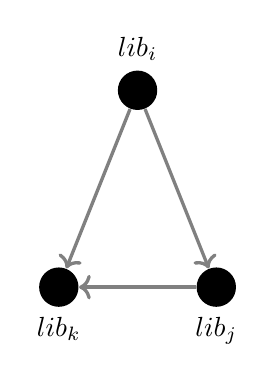
\begin{tikzpicture}[
         roundnode/.style={circle, fill=black, minimum size=5mm},
        squarenode/.style={fill=black, text=red, minimum size=5mm},
     ]
    \begin{scope}
         \node[roundnode, label=above:$lib_i$] (s2_proji) at (3, 2.5) {};
        \node[roundnode, label=below:$lib_j$] (s2_projj) at (4,0) {};
         \node[roundnode, label=below:$lib_k$] (s2_projk) at (2,0) {};
     \end{scope}

     \begin{scope} [every edge/.style={draw=gray, very thick}]
         \path [->] (s2_proji) edge (s2_projj);
         \path [->] (s2_proji) edge (s2_projk);
         \path [->] (s2_projj) edge (s2_projk);
     \end{scope}
     \end{tikzpicture}
    
     \caption{Example dependency graph for a given time period}
     \label{fig:lib}
     \vspace{2ex}
 \end{figure}
\begin{figure}[t]
    \centering

    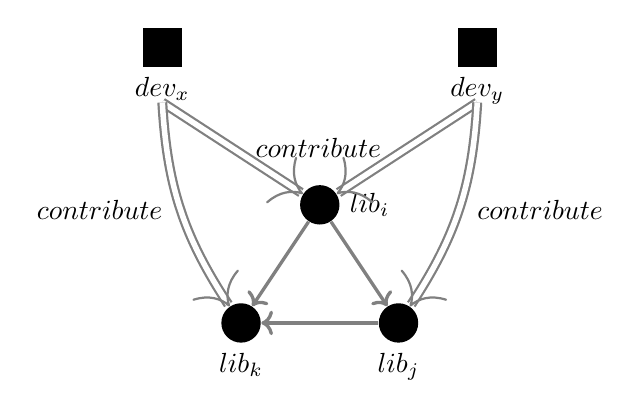
\begin{tikzpicture}[
        roundnode/.style={circle, fill=black, minimum size=5mm},
        squarenode/.style={fill=black, text=red, minimum size=5mm},
    ]
    \begin{scope}
        
        \node[roundnode, label=right:$lib_i$] (s2_proji) at (4, 1.5) {};
        \node[roundnode, label=below:$lib_j$] (s2_projj) at (5,0) {};
        \node[roundnode, label=below:$lib_k$] (s2_projk) at (3,0) {};
        
        \node[squarenode, label=below:$dev_x$] (s3_devx) at (2, 3.5) {};
        
        \node[squarenode, label=below:$dev_y$] (s3_devy) at (6, 3.5) {};
        
    \end{scope}

    \begin{scope} [every edge/.style={draw=gray, very thick}]
        \path [->] (s2_proji)  edge  (s2_projj);
        \path [->] (s2_proji) edge (s2_projk);
        \path [->] (s2_projj) edge (s2_projk);
        
    \end{scope}
    \begin{scope} [every edge/.style={draw=gray, thick, double distance=2pt}]
        \path [->] (6, 2.8) edge node[left = 2mm] {$contribute$} (s2_proji);
        \path [->] (6, 2.8) edge[bend left=15] node[right = 1mm] {$contribute$} (s2_projj);
        \path [->] (2, 2.8) edge node[right = 2mm] {$$} (s2_proji);
        \path [->] (2, 2.8) edge[bend right=15] node[left = 1mm] {$contribute$} (s2_projk);
    \end{scope}
    \end{tikzpicture}
\end{figure}
\begin{figure}[t]
    \centering
    \begin{tikzpicture}[
        roundnode/.style={circle, fill=black, minimum size=5mm},
        squarenode/.style={fill=black, text=red, minimum size=5mm},
    ]
    \end{tikzpicture}
\caption{Example Dependency-Contribution graph showing relationships between contributions and dependencies}
 \label{fig:dc-graph}
\end{figure}

This is just one example of the type of research that is enabled by access to heterogeneous data related to software package ecosystems.

\smallskip\noindent\textbf{Peril 1.}\textit{
 Developers might use different identifiers when contributing to different parts of a software package ecosystem, e.g., when contributing to different libraries.}\\
 
When modelling using such graphs, there is a threat that contributors may use multiple identifiers (i.e., $c_x$ and $c_y$ are the same contributor).
This is a well-known research problem, and there has been work to merge these accounts, such as \cite{wiese2016mailing}.
GitHub has introduced mechanisms such as two-factor authentication\footnote{\url{https://docs.github.com/en/authentication/securing-your-account-with-two-factor-authentication-2fa/configuring-two-factor-authentication}} to counteract the issue of multiple identifiers.
This is since developers might be less likely to switch accounts if it requires cumbersome authentication.


\smallskip\noindent\textbf{Peril 2.}\textit{
Developers' contributions to software package ecosystems might be interspersed with bot contributions, e.g., automated dependency updates.}\\

The rise of automation and artificial intelligence has led to much work on the integration of automated scheduling (i.e., bots) into software development workflows \cite{Storey2016, Farooq2016, Wessel2018, Erlenhov2019, bot_modify_wf} to name a few. These bots are designed to perform specific tasks within a software package ecosystem. For example, a bot may be programmed to automatically update dependencies, test code changes, or deploy software to production. As an example, the Google APIs repo-automation-bots project lists bots for automated labelling of issues and pull requests, automated approval of pull requests, and triggering releases.\footnote{\url{https://github.com/googleapis/repo-automation-bots}}
Bots perform common maintenance tasks in many software projects and are now commonplace \cite{Beschastnikh2017, Urli2018,BIMAN,bot_or_not}.
Especially with bots such as dependabot (automated pull requests to update configurations to reduce the risk of vulnerability threats),\footnote{\url{https://github.com/dependabot}} more and more automation has caused a lot of noise in the contributions between projects.
There are also bots for communication and documentation \cite{Urli2018, Lin2016, Lebeuf2017a}.

To be able to draw accurate conclusions about what humans are doing in software package ecosystems, researchers should consider distinguishing between bot and human contributions.
It is also important to differentiate this from other contributions \cite{maeprasart2022understanding}.
The research community has responded well, with a wide range of techniques and tools to mitigate this peril \cite{Bodegha2021, golzadeh2022accuracy}.

\smallskip\noindent\textbf{Peril 3.}\textit{
Not all developer activities in software package ecosystems are accessible to the public, e.g., library use in proprietary settings.
}\\

Not all developer activities in software package ecosystems are accessible to the public, e.g., when the boundary between open source and industry is blurred \cite{stol2014inner}, which presents a challenge for researchers who aim to study the development process. This is particularly true in proprietary settings where software development is performed behind closed doors or is open source for a limited time period, thus resulting in the artefacts not permanently being publicly available.
This can make it difficult to understand the broader ecosystem in which a software project is developed.
Proprietary settings may lead to non-standardisation in software development practises. Different software projects may use different management systems and tools, making it difficult to accurately compare and analyse software development activities across various projects. For example, some projects may use communication, documentation, and other management tools not captured on the same platform \cite{montgomery2022alternative}. For example, some projects might use Bugzilla instead of issues and pull requests for their bug and code review systems, while others may use Discord, Slack channels, or email threads for their communication needs.

This lack of standardisation in software development practises presents a challenge for researchers who study the software package ecosystem and understand the development process. To address this issue, researchers should strive to collect data from a diverse set of projects to gain a comprehensive understanding of the software package ecosystem. In addition, researchers may need to adjust their methodologies or data collection techniques to accommodate the different tools and practises used by different software projects.

\subsection{Defining Components and their Dependencies}

\smallskip\noindent\textbf{Promise 2.}\textit{
Researchers can access a software package ecosystem's dependency network through package managers and registries, e.g., npm lists the dependencies and dependents for over a million libraries.}\\


With the rise of curated datasets like libraries.io, researchers can now recover and model dependency relations between software units using pre-extracted datasets.
Table \ref{tab:PM_features} shows examples of popular package managers mined from the libraries.io dataset in 2020. 

\begin{table*}[]
\caption{Summary of 13 package managers from libraries.io as ranked by TIOBE in 2020}
 \label{tab:PM_features}
 \centering
\begin{tabular}{@{}llrlll@{}}
\toprule
\begin{tabular}[c]{@{}l@{}}Package \\ Ecosystem\end{tabular} & \begin{tabular}[c]{@{}l@{}}Programming \\ Language\end{tabular} &  \begin{tabular}[c]{@{}l@{}}Tiobe \\ Rank\end{tabular} & Environment & \begin{tabular}[c]{@{}l@{}}Dependency \\ Tree\end{tabular} & \begin{tabular}[c]{@{}l@{}}Package   \\Archive link\end{tabular}\\ \midrule
PyPI & Python & 2 & Python & Flat & pypi.org  \\
Maven & Java & 3 & JVM & Flat & Maven.org  \\
Bower & JavaScript & 7 & Node.js & Flat & bower.io  \\
Meteor & JavaScript & 7 & Node.js & Nested & atmospherejs.com \\
npm & JavaScript & 7 & Node.js & Nested (v2) & npmjs.com  \\
Packagist & PHP & 8 & PHP & Flat & packagist.org \\
Puppet & Ruby & 13 & Ruby MRI & Flat & forge.puppet.com  \\
RubyGems & Ruby & 13 & Ruby MRI & Flat & rubygems.org  \\
CRAN & R & 14 & RStudio & Flat & cran.r-project.org  \\
CPAN & Perl & 15 & Perl & Flat & metacpan.org  \\
GO & Golang & 20 & Go & Flat & pkg.go.dev  \\
NuGet & C\#, VB & 5, 6 & .NET & Flat & nuget.org \\
Anaconda & Python, R, C\# & 2, 14, 5 & Anaconda & Flat & anaconda.org  \\ \bottomrule
\end{tabular}
\end{table*}

\smallskip\noindent\textbf{Peril 4.}\textit{
Different software package ecosystems define the concept of ``dependency'' differently, e.g., by allowing or not allowing different versions of a library on the same dependency tree.
}\\

Different software package ecosystems have varying definitions of what constitutes a dependency. For example, some ecosystems may allow multiple versions of a library to exist on the same dependency tree, while others may restrict developers to a single version of a library \cite{Islam}. These restrictions are often based on the programming language being used, as different languages have different approaches to managing dependencies. It is important to consider the restrictions on dependency relationships when studying software package ecosystems, as they can have a major impact on the development process. For example, the ability to use multiple versions of a library on the same dependency tree can greatly simplify the process of updating dependencies and can make it easier to resolve conflicts between libraries.

One way to visualise the impact of these restrictions is to compare the difference between a nested dependency tree and a directed dependency tree, as shown in Figure \ref{fig:nest}.\footnote{Taken from \url{https://npm.github.io/how-npm-works-docs/npm3/how-npm3-works.html}} This distinction is important because it highlights the different ways that a software unit can depend on different versions of the same library.
In this example, npm v3 creates the dependency tree based on the installation order, therefore flattening unnecessary nested dependencies (i.e., B v1.0 in cyan). This reduces the complexity of a nested tree by resolving some of the transitive dependencies (nested dependencies).

\begin{figure}
	\centering
	\includegraphics[width=.8\textwidth]{book/chapter-promisesandperils/pics/nestedv2.jpg}
	\caption{Difference between flat and nested dependencies}
	\label{fig:nest}
\end{figure}

\smallskip\noindent\textbf{Peril 5.}\textit{
Developers might declare a dependency to other parts of a software package ecosystem but not use it, e.g., because they failed to update its removal.
}\\

It is common for developers to declare dependencies on other parts of the software package ecosystem but not always use them. This can happen for various reasons, such as forgetting to remove the dependency after it is no longer needed. This can pose a challenge for researchers who are trying to extract dependencies from package managers, like those in configuration files, as there may be inconsistencies between the listed dependencies and what is actually being compiled and used by the code. This can lead to a biased understanding of the software package ecosystem and the relationships between software components.

To address this issue, there have been numerous efforts to track the actual library dependencies compiled and executed in software systems. These efforts aim to provide a more accurate understanding of the dependencies and the relationships between software components. For example, research has been conducted on the use of dynamic analysis to track compiled dependencies in real time and on the development of tools to automatically detect and track executed dependencies \cite{Zapata:ICSME2018, Ponta2018,Chinthanet:ASE2020}.

\subsection{Defining Boundaries and Completeness}

\smallskip\noindent\textbf{Promise 3.}\textit{
Researchers can use the boundaries of software package ecosystems to study communities of developers, e.g., developers contributing to and/or benefiting from the npm ecosystem.
}\\

Following Promise 2, the emergence of package managers has also led to studies that approximate software communities.
Using the libraries.io dataset, researchers were able to study projects that host libraries that use package managers.
Researchers have used this dataset to compare different library ecosystems \cite{kikas.2017,decan:emse:2019,CogoDown2019}.


\smallskip\noindent\textbf{Peril 6.}\textit{
Package managers do not always represent software package ecosystems, their communities, or their sub-communities, e.g., in cases where multiple package managers exist.
}\\

Package managers are a fundamental aspect of software package ecosystems, but do not always fully represent the complex relationships and interactions that occur within a community of developers and users, as shown in Table~\ref{tab:PM_features}. In some cases, multiple package managers exist for the same programming language, creating a complex landscape of software libraries and dependencies that are not always easily understood. For instance, Bower and Meteor manage npm libraries, which can lead to confusion and overlap in the management of dependencies.

Similarly, Java, Scala, Android, and other Java-based open source communities all use the Maven package manager, but each of these communities has its own unique set of libraries, dependencies, and development practises. Researchers should be aware of the limitations of package managers when studying software package ecosystems, and consider the broader context and relationships that exist within these communities. 

\smallskip\noindent\textbf{Peril 7.}\textit{
Lack of activity in parts of a software package ecosystem does not necessarily indicate project failure, e.g., when highly depended-upon libraries are feature-complete.
}\\

It is important to note that lack of activity in a part of a software package ecosystem does not always mean project failure \cite{coelho2017modern}. In some cases, highly relied-upon libraries that have reached feature-completeness may see little activity, but continue to be used by the software community. 

However, it is still important to consider the long-term sustainability of these libraries, especially given the rate at which technology and software development practises change. This has become a topic of interest in recent years, and researchers have explored best practises for sustaining open source projects and ensuring their continued success \cite{Ait2022,valiev2018ecosystem}. Understanding the factors that contribute to project sustainability is important to ensure the longevity and continued growth of software package ecosystems.

\smallskip\noindent\textbf{Peril 8.}\textit{
Sampling from a software package ecosystem is challenging since sub-setting might alter the dependency network, e.g., by breaking dependency chains.
}\\

Sampling from a package ecosystem is not straightforward, as the sample composition can be significantly affected due to missing dependency links between libraries. For instance, a subset of the ecosystem might alter the dependencies between libraries, leading to the breakdown of the dependency chains. This could lead to an incomplete picture of the software package ecosystem, leading to incorrect conclusions from a study. To minimise this risk, researchers should carefully consider the boundaries of their study and choose the appropriate sampling method based on the research questions and goals. For example, researchers could focus on popular, highly dependent, or risk-vulnerable aspects of the ecosystem as a starting point. 
For some ecosystems, the number of downloads, GitHub stars, and watchers are other aspects for the researcher to utilise.


\smallskip\noindent\textbf{Peril 9.}\textit{
Sampling from a software package ecosystem is challenging since the dependency network changes over time, e.g., when dependencies are added, removed, upgraded, or downgraded.
}\\

The dynamic nature of package ecosystems and the constant changes to their dependencies can impact the generalisability of the results. Therefore, it is important to also consider the time granularity of the analysis. For example, if the goal is to understand the evolution of dependencies over time, a finer time granularity may be necessary to capture the smaller changes and trends. However, if the goal is to understand the overall structure and relationships within the ecosystem, a coarser time granularity may be sufficient. Based on recent studies \cite{wattanakriengkrai2022giving,valiev2018ecosystem,Mirsaeedi:icse2020, Brindescu:emse2020, Nassif:icsme2017}, a three-month window seems appropriate for some studies.
Another level of granularity to consider is the size of the component. For instance, there are cases where a single package may contain more than one repository, especially for large library frameworks. 
The granularity also depends on the nature of the ecosystem itself. For instance, researchers should understand whether the ecosystem comprises library packages (e.g., PyPI), plugins (e.g., Eclipse), or is a library distribution (e.g., Android).



\subsection{Analysing and Visualising the Data}

\textbf{Peril 10.}\textit{
Analysing and visualising entire software package ecosystems is challenging due to their size, e.g., in terms of nodes and edges in the network.
}\\

The size of software package ecosystems implies large data sets, which can be overwhelming for tools and algorithms to analyse and display. Therefore, it may be necessary to make choices about the granularity of the data included in the analysis and visualisation. Another alternative is to focus on the most critical parts of the software package ecosystem, such as the high-level structure, highly dependent packages, or parts of the system that pose a risk to security and reliability. 
The key is to strike a balance between detail and simplicity, providing a meaningful representation of the ecosystem while being able to handle the complexity of its size.


\section{Application: When to Apply Which Peril}
\label{PPM:sec:application}

We include a disclaimer stating that not all perils are applicable to every mining situation. To demonstrate the practical application of our perils and their mitigation, we present two case studies that involve mining the software package ecosystem. Each case study has a distinct research objective and focusses on a specific dataset to be mined.

\subsection{Two Case Studies}
Table \ref{tab:cases} presents the two case studies we have selected for this analysis.
The \textit{first case} involves mining for contributions congruent to dependency updates \cite{wattanakriengkrai2022giving}. 
In this work, the authors mine GitHub repositories for Pull Requests and Issues that were submitted and merged congruent to dependency updates within the npm ecosystem. 
The \textit{second case} involves mining communication data for the Eclipse ecosystem \cite{Nugroho2021}. Although the second case does not mine for dependency relations (i.e., use relations),  we show that these perils still apply when mining for other relationships in an ecosystem.
Moreover, the second case studies the Eclipse ecosystem, which is a different dataset compared to the more popular GitHub dataset.

\subsection{Applying Perils and their Mitigation Strategies}
Table \ref{tab:perilsapp} provides a summary of the perils that can be applied to each of the case studies. We will now go into the details of mitigation strategies based on these perils. 
For better organisation and understanding, we have grouped the perils according to the four logical processes for mining.

\smallskip\noindent\textbf{Information to Mine}. 
The first set of mitigation strategies, which addresses perils 1-3, focusses on planning which information to mine. There are two primary strategies that researchers can employ:


\begin{enumerate}
    \item Researchers should use research tools and techniques to remove noise and other biases in the dataset, such as bot detection and the handling of multiple identities. This strategy was implemented in both case studies, as contributions and discussions often have the potential to involve bots or developers with multiple identities.
\item Depending on the research goals, researchers should recognise that not all contributions are equal and filter the dataset accordingly.
\end{enumerate}

We applied these two strategies to both cases. In the first case, the goal was to capture all congruent contributions, so we filtered out contributions made to libraries without dependencies. Since all npm packages are listed in the registry, Peril 3 (private activities) did not apply.
In the second case, we addressed Peril 1 by conducting a qualitative analysis to ensure that the member identities were not duplicated, as Eclipse developers were known to change identities. To mitigate Peril 2, we removed bot responses. For the second case, since all forum data is made public, Peril 3 did not apply.


\begin{table}
\centering
\caption{Description of the research objectives and datasets for the case studies}
 \label{tab:cases}
\begin{tabular}{lp{5cm}r} 
\toprule
\textbf{Case Study} & \textbf{Research Objective}                                                          & \textbf{Datasets}           \\
\midrule
Wattanakriengkrai \etal \cite{wattanakriengkrai2022giving}             & Explore code contributions between library and client (i.e, use-relations)  & libraries.io\\
& &  GitHub API \\
Nugroho \etal \cite{Nugroho2021}                & Explore discussion contributions between contributors (i.e., contributions) & Eclipse API                \\
\bottomrule
\end{tabular}
\end{table}

\begin{table}
\centering
\caption{Application of each peril to the case studies}
 \label{tab:perilsapp}
\begin{tabular}{rp{8cm}ccc} 
\toprule                   
& \textbf{Perils}       & case 1      & case 2                 \\
                                                                               & & npm  & Eclipse   \\
\midrule
\textbf{P1} &Developers might use different identifiers when contributing to different parts of a software package ecosystem, e.g., when contributing to different libraries.                             &    \CheckedBox         &          \CheckedBox           \\ 
%\hline
\textbf{P2} & Developers' contributions to software package ecosystems might be interspersed with bot contributions, e.g., automated dependency updates.                                                      &      \CheckedBox               &      \CheckedBox               \\ 
%\hline
\textbf{P3} & Not all developer activities in software package ecosystems are accessible to the public, e.g., library use in proprietary settings.                                                         &         -           &      \CheckedBox               \\ 
%\hline
\textbf{P4} & Different software package ecosystems define the concept of \`{}\`{}dependency'' differently, e.g., by allowing or not allowing different versions of a library on the same dependency tree. &         \CheckedBox       &     -                            \\ 
%\hline
\textbf{P5} & Developers might declare a dependency to other parts of a software package ecosystem but not use it, e.g., because they failed to update its removal.                                        &     -           &  -    \\
%\hline
\textbf{P6} &Package managers do not always represent software package ecosystems, their communities, or their sub-communities, e.g., in cases where multiple package managers exist.                     &     -                   &  -                  \\
%\hline
\textbf{P7} & Lack of activity in parts of a software package ecosystem does not necessarily indicate project failure, e.g., when highly depended-upon libraries are feature-complete.                     &       \CheckedBox         &  -                           \\
%\hline
\textbf{P8} &Sampling from a software package ecosystem is challenging since sub-setting might alter the dependency network, e.g., by breaking dependency chains.                                         &        \CheckedBox        &     \CheckedBox                                \\
%\hline
\textbf{P9} &Sampling from a software package ecosystem is challenging since the dependency network changes over time, e.g., when dependencies are added, removed, upgraded, or downgraded.               &       \CheckedBox         &     -                          \\
%\hline
\textbf{P10} &Analysing and visualising entire software package ecosystems is challenging due to their size, e.g., in terms of nodes and edges in the network.                                  &        \CheckedBox      &      \CheckedBox               \\
\bottomrule
\end{tabular}
\end{table}

\smallskip\noindent\textbf{Defining Dependencies}. 
The second set of perils (Perils 4-5) is related to dependency relationships between software units, and only the first case study is applicable. To address these perils, researchers should adopt the following strategy:

\begin{enumerate}
    \item Researchers should not rely solely on listed dependencies in configuration files (e.g., pom.xml, package.json, etc.) as a measure of dependency between two components. Instead, code-centric approaches should be used to validate which libraries are actually depended upon.
\end{enumerate}

For example, in the first case, in addition to mining the configuration information, the authors also analysed the similarity of the source code contributions to address Peril 4. Regarding Peril 5, since the study's objective was to investigate changes to the configuration files, the risk of the update not being executed was deemed less important.
It is important to note that the second case study did not include dependency analysis and, therefore, these perils did not apply.

\begin{figure*}[]
    \centering
    \begin{subfigure}{0.9\linewidth}
         \includegraphics[width=1.1\textwidth]{book/chapter-promisesandperils/pics/congruentViz.jpg}
         \caption{Visualization of a Time analysis for 107,242 libraries.}
     \end{subfigure}
     \begin{subfigure}{0.9\linewidth}
         \includegraphics[width=1\textwidth]{book/chapter-promisesandperils/pics/eclipseViz.jpg}
         \caption{A Visual Topology map for 832,058 threads}
     \end{subfigure}
    \caption{Visualisation examples for the two case studies}
    \label{fig:visCase}
\end{figure*}

\smallskip\noindent\textbf{Defining Boundaries}.
The third set of perils (Perils 6-9) is related to the definition of boundaries and completeness and is relevant for both case studies. To mitigate these perils, we recommend the following strategies:

\begin{enumerate}
    \item Researchers should recognise that a dormant project does not necessarily mean that it is inactive. Instead, studies can use alternative heuristics, such as the number of dependents and dependencies, as better indicators of a project's importance in the ecosystem.
    \item Researchers should not rely solely on the programming language to define sub-communities. Using a common package manager for the programming language is a more effective rule of thumb for distinguishing boundaries.
    \item Researchers should avoid random sampling. Instead, sampling should be tailored to the research goals by considering factors such as an appropriate time window or focussing on specific attributes of components (e.g., most dependents, most popular, most contributors).
\end{enumerate}


Peril 6 did not apply to any of the case studies. 
Particularly for the first case, since the goal was to explore the npm package ecosystem, we assumed that the boundaries were clearly defined by the npm registry. 
Similarly, the second case study used the generic Eclipse platform as the boundary. 
Peril 7 was applied to the npm study, while Peril 8 was applied to both case studies. 
As a result, the two cases conducted a qualitative analysis of the dataset to gain deeper insights.
In the first case study, a three-month time window was created to capture dependencies. 
For the second case study, forum contributors were sampled into three groups (i.e., junior, member, or senior) according to the sliding window of their contributions. 

\smallskip\noindent\textbf{Visualisation}.
The final peril (Peril 10) relates to visualisation, which can be challenging due to the vast size and complexity of software ecosystems. As it is not feasible to visualise every aspect of an ecosystem simultaneously, a focused approach is necessary. A mitigation strategy is to select specific attributes of the ecosystem (e.g., the most dependent, most popular, and most contributions) that align with the research needs and objectives. 

Figure \ref{fig:visCase} shows two cases where visualizations are employed to gain insights, especially for large datasets.
In the first figure (a), we visualize the distributions of the data set and applied the appropriate statistical tests, along with the effect size, to test our hypotheses and answer research questions. 
In the second example (b), although not directly related to package ecosystems, the authors utilized a topological visualization \cite{Lum2013ExtractingIF} to gain insights on the over 800,000 forum threads of discussions. 



\section{Chapter Summary}
In this chapter, we explore the various aspects of mining information from the software package ecosystem, presenting three promises and ten perils that researchers should be aware of when undertaking such tasks. The chapter is structured around four key processes for mining: 1) Planning what Information to Mine, 2) Defining Components and their Dependencies, 3) Defining Boundaries and Completeness, and 4) Analysing and Visualising the Data. To help new and experienced researchers navigate these challenges, we introduced the SUG model, which can serve as a valuable tool to minimise threats to validity. Although some perils may be more relevant to specific research objectives, our aim is to equip researchers with the knowledge and resources needed to confidently gather and integrate software package ecosystem data into their work.
%An Introduction to Software Development Ecosystems
%Semantic labeling three-letter-code: INT (e.g. \chapter{INT})

% 
\title{Promises and Perils of Mining \\ Software Package Ecosystem Data}
\author{Raula Gaikovina Kula \and Katsuro Inoue \and Christoph Treude}
\institute{Raula Gaikovina Kula \at Nara Institute of Science and Technology, Japan, \email{raula-k@naist.jp}
\and Katsuro Inoue \at Nanzan University, Japan \email{ inoue599@nanzan-u.ac.jp}
\and  Christoph Treude \at The University of Melbourne, Australia \email{christoph.treude@unimelb.edu.au}}

\maketitle
\label{PPM:ch}
\abstract*{The use of third-party packages is becoming increasingly popular and has led to the emergence of large software package ecosystems with a maze of inter-dependencies. Since the reliance on these ecosystems enables developers to reduce development effort and increase productivity, it has attracted the interest of researchers: understanding the infrastructure and dynamics of package ecosystems has given rise to approaches for better code reuse, automated updates, and the avoidance of vulnerabilities, to name a few examples. But the reality of these ecosystems also poses challenges to software engineering researchers, such as: How do we obtain the complete network of dependencies along with the corresponding versioning information? What are the boundaries of these package ecosystem? How do we consistently detect dependencies that are declared but not used? How do we consistently identify developers within a package ecosystem? How much of the ecosystem do we need to understand to analyse a single component? How well do our approaches generalise across different programming languages and package ecosystems? In this chapter, we review promises and perils of mining the rich data related to software package ecosystems available to software engineering researchers.}

\abstract{The use of third-party packages is becoming increasingly popular and has led to the emergence of large software package ecosystems with a maze of inter-dependencies. Since the reliance on these ecosystems enables developers to reduce development effort and increase productivity, it has attracted the interest of researchers: understanding the infrastructure and dynamics of package ecosystems has given rise to approaches for better code reuse, automated updates, and the avoidance of vulnerabilities, to name a few examples. But the reality of these ecosystems also poses challenges to software engineering researchers, such as: How do we obtain the complete network of dependencies along with the corresponding versioning information? What are the boundaries of these package ecosystems? How do we consistently detect dependencies that are declared but not used? How do we consistently identify developers within a package ecosystem? How much of the ecosystem do we need to understand to analyse a single component? How well do our approaches generalise across different programming languages and package ecosystems? In this chapter, we review promises and perils of mining the rich data related to software package ecosystems available to software engineering researchers.}

%%%%%%%%%%%%%%%%%%%%%%%%%%%%%%%%%%%%%%%%%%%%%%%%%%%%%%%%%%%%%%%%%%

\section{Introduction}
\label{PPM:sec:definition}

Third-party libraries are a great way for developers to incorporate code without having to write their own for every functionality required. By using these libraries, developers can save time and energy while still getting the functions they need.
Using third-party libraries is becoming increasingly popular and has led to the emergence of large software package ecosystems such as npm. While these ecosystems offer many benefits, they also come with risks, such as software vulnerability attacks \cite{Chinthanet:ASE2020}.

Large software package ecosystems are a treasure trove for researchers who can investigate a wide range of questions. For example, by studying activity in large ecosystems, researchers can identify which libraries are the most popular and learn what characteristics make them successful \cite{kikas.2017,decan:emse:2019}.
Additionally, research on large ecosystems can help developers understand how to protect their code from malicious actors who may attempt to exploit vulnerabilities or insert malware into popular libraries.
Studying large software package ecosystems can help us better understand the dynamics of open source development in general. Open source development is a complex process that involves many different stakeholders working together (or sometimes competing) to create valuable code that anyone can use or improve upon. By understanding how these interactions play out in different types of ecosystem structures -- including those with many small projects versus few very large ones -- we can develop insights that might be applicable more broadly across other types of collaborative systems.

In this chapter, we identify and discuss promises and perils during the mining process, ranging from planning what information to mine from the ecosystem to analysing and visualising the mined data. 
Therefore, the chapter is broken down into these logical processes of mining ecosystem data: 1) Planning what Information to Mine, 2) Defining Components and their Dependencies, 3) Defining Boundaries and Completeness, and 4) Analysing and Visualising the Data.

This chapter is intended for researchers and practitioners who are interested in exploring and exploiting software package ecosystem information from a diverse range of sources that are publicly available. 
We also highlight the pitfalls to consider during the mining process, particularly when these pitfalls could lead to a misinterpretation of the analysis and results. 
The chapter is written in a manner that encourages newcomers who have little or no experience or who are interested in utilising ecosystem data across different disciplines outside of software engineering.
Our goal is to get new researchers quickly accustomed to gathering ecosystem information for their research.


\section{A Component-based Software Ecosystem}

Defined as a component-based software ecosystem, we suggest using the term `software package ecosystem' as a suitable term for the symbiotic relationships among third-party library components (as software projects or repositories), as these libraries and their dependent clients coexist on the same technological platform, therefore sharing the same environment and other internal and external factors (e.g., security threats, sharing contributions, etc.).
Please refer to the Introduction chapter for an in-depth definition of the different types of software ecosystems.
We present our interpretation of the software package ecosystem in Kula et al.~\cite{KulaSANER18}, where we formally define a package ecosystem using a Software Universe Graph (SUG).
This is modelled as a structured abstraction of the evolution of software systems and their library dependencies over time.

%%%%%%%%%%%%%%%%%%%%%%%%%%%%%%%%%%%%%%%%%%
\begin{figure*}
	\centering
	\includegraphics[width=.7\textwidth]{book/chapter-promisesandperils/pics/UniversalExample.jpg}
	\caption{Conceptual example of the Software Universe Graph, depicting the use and update relationships between different software units.}
	\label{fig:SUG}
\end{figure*}
%%%%%%%%%%%%%%%%%%%%%%%%%%%%%%%%%%%%%%%%%%%%%


\paragraph{\textbf{Component-based Representation as a Software Universe Graph}}
\label{PPM:sec:SUG}

First introduced by Kula et al.~\cite{KulaSANER18}, the \textit{Software Universe Graph} (SUG) is a structural abstraction of the software ecosystem of third-party libraries.
Figure \ref{fig:SUG} provides an illustration of the different relationships within the graph.
Let $G= (N,E)$ represent a graph $G$. $N$ is a set of nodes, each node representing a software unit. 
We define a software unit as a version instance of any software program. 

The authors then present the \textit{use} and \textit{update} relationships that exist in the ecosystem.
Hence, the edges $E$ are composed of $E_{use}$ and $E_{update}$. $E_{use}$ is a set of \textit{use-relations} and $E_{update}$ is a set of \textit{update-relations}.

\begin{definition}
An edge $u \rightarrow v \in E_{use}$ means that $u$ uses $v$. The defined functions of $E_{use}$ are:

\begin{equation}
\small
\small \use(u)\equiv \{v|u \rightarrow v\}
\normalsize
\end{equation}
\begin{equation}
\small
\small \useBy(u)\equiv \{v|v \rightarrow u\}
\normalsize
\end{equation}
\end{definition}

Use-relations can be extracted from either the source code or configuration files. 
As shown in Figure \ref{fig:SUG}, node $a1$ uses node $x1$. 
In addition, node $x1$ is used by nodes $a1$, $q1$, and $q2$. Parallel edges for node pairs are not allowed.

\begin{definition}
We represent an update relation from node $a$ to $b$ using $ a \Rightarrow b $, which means that the newer update $b$ was released from node $a$ and is defined as:
\begin{equation}
\small a \Rightarrow b \in E_{update}
\end{equation}
\end{definition}

Update relations refer to when a successive release of a software unit is made available. Figure \ref{fig:SUG} shows that node $q1$ is first updated to node $q2$. Later, node $q2$ is updated to the latest node $q3$. Hence, $q1 \Rightarrow q2 \Rightarrow q3$.
Note that an update should not be confused with forking. 
We distinguish a fork as a separate software unit. 
Each node in the SUG should be denoted by three attributes: \texttt{<name,release,time>}.  
For a node $u$, we define:

\begin{itemize}
	\item \textbf{u.name} Name is the string representation identifier of a software unit.
	We introduce the name axiom: For nodes $u$ and $v$, if $u \Rightarrow v$, then $u.name = v.name$ holds.
	
	\item \textbf{u.release}. Release refers to the specific assigned change reference for a software unit. For nodes $u$ and $v$, if $u \Rightarrow v$
	then $v$ is the immediate successor of $u$. Note that the versioning pattern may vary from project to project. 
	\item \textbf{u.time}. Time refers to the time stamp at which node $u$ was released. For nodes $u$ and $v$ of $u \Rightarrow v$, $u.time < v.time$.
\end{itemize}

\begin{figure}
	\centering
	\includegraphics[width=.8\textwidth]{book/chapter-promisesandperils/pics/TemporalSUG.jpg}
	\caption{Temporal property of the SUG}
	\label{fig:SUGTemp}
\end{figure}

\begin{definition}
    
	The SUG has temporal properties.
This describes the simultaneity or ordering in reference to time. Let SUG $G = (N, E) $ be at time $t$. At time $t^{\prime} > t$, we observe an extension of $G$, such that:

\begin{equation}
\small G^{\prime} = (N \cup \Delta N, E \cup \Delta E)
\end{equation}
where $\Delta E \cap (N \times N) = \emptyset$
\end{definition}

Figure \ref{fig:SUGTemp} illustrates the temporal properties of the SUG. 
Here, it is observed that $G'$ is composed of $G$ augmented with newly added node $a3$ and its corresponding $a3 \rightarrow x2$ and $a2 \Rightarrow a3$ relations.
A SUG grows monotonically over time with only additions.
Here, we consider that modification or deletion changes on the SUG do not occur. 

\begin{definition}
    A timed SUG specifies the state of the SUG at any point in time.
So for an SUG $G=(N,E)$, we represent a timed SUG $G_{t}$ at time $t$ as a sub-graph of $G$. Formally,
\begin{equation}
\small G_t\equiv(N_{t}, E_{t})
\end{equation}
where $N_{t} = \{u|u \in N, u.time \leq t \}$ and $E_t = \{ e | e \in E \wedge e \in  N_t \}$
\end{definition}
	


\section{Data Sources}
Researchers can use various datasets to model the ecosystem using the SUG model of usage and update relationships.
The most obvious data source that has revolutionised data mining in the software engineering domain is the GitHub platform. 
Established in 2008, and then purchased by Microsoft in 2020, GitHub is home to various popular Open Source Software. 
GitHub is built on the git version control system and is useful for storing all changes made to a repository. 
In the case of the SUG, a GitHub repository can represent one software unit, whose depend relations can be extracted via a configuration file (such as the package.json file for JavaScript projects).
The repository should also contain the release information that holds the update relations.
Due to its large size, researchers and the GitHub team have made available datasets for researchers to mine, for example through the GitHub API/Graph QL.\footnote{\url{https://docs.github.com/en/graphql}} This is the backend Application Programming Interface (API) that can be used to query large amounts of data on GitHub. Most researchers use the API to download and mine information from the GitHub platform. 
It is important to note that while GitHub introduced a new feature of Dependency Graphs to map the depend relationship,\footnote{\url{https://docs.github.com/en/code-security/supply-chain-security/understanding-your-software-supply-chain/about-the-dependency-graph}} most older projects do not have this feature.
In this case, the researcher would need to manually extract and query the configuration files for dependency information. 

We refer to the first chapter for additional information on data sources for mining software ecosystems. 

\section{Promises and Perils}
\label{PPM:sec:promisesperils}

Using the SUG model of depend and use relations and the available datasets, we can now present our promises and perils of mining ecosystem information.

\subsection{Planning What Information to Mine}

\textbf{Promise 1.}\textit{
Researchers can access and link heterogeneous data related to software package ecosystems, e.g., package registries and bug trackers.}\\

When planning what information to mine from the ecosystem, researchers do not need to limit themselves to the usage and update relationship information.
Platforms that host software repositories include other software management systems such as bug trackers.
For example, GitHub allows researchers to manage GitHub Pull Requests, Issues, and Discussions not only for one project, but for multiple projects.
GitHub provides three management systems that are related to a software repository:

\begin{itemize}
    \item \textit{GitHub Discussions}\footnote{\url{https://docs.github.com/en/discussions}} - The GitHub Discussions forum is a collaborative communication forum for the community around an open source or internal project. Community members can ask and answer questions, share updates, have open-ended conversations, and follow along on decisions affecting the community's way of working.
    \item \textit{GitHub Pull Requests}\footnote{\url{https://docs.github.com/en/pull-requests}} - Pull Requests allow other developers from an ecosystem to make a contribution to a software repository. Pull requests also allow maintainers to discuss and review potential changes with collaborators and add follow-up commits before changes are merged into the software.
    \item \textit{GitHub Issues}\footnote{\url{https://docs.github.com/en/issues}} - Issues are used to track ideas, feedback, tasks, or bugs for work on GitHub.
\end{itemize}

These three systems are examples of how developers contribute to both their own and other projects. 
Hence, to incorporate this information, we can extend the SUG model, creating a model that includes a contribution relationship \cite{wattanakriengkrai2022giving}.

% Note that other platforms may also have management systems, like GitLab, BitBucket and Eclipse.

\begin{definition}
	A Dependency-Contribution graph incorporates contributions by developers whose libraries are involved in dependency relationships. 
\end{definition}

In this work \cite{wattanakriengkrai2022giving}, the authors explore the congruence between dependency updates and developer contributions, based on the original concept of social-technical congruence \cite{stcCataldo2008} where developers contribution patterns are congruent with their coordination needs. Hence, the goal is to identify contributions that are congruent to dependency updates.
As shown in Figure \ref{fig:lib} the authors extend from the typical SUG graph model where $lib_i$ depends (use) on  $lib_k$ and  $lib_j$, while  $lib_j$ also depends on $lib_k$, to the example shown in Figure \ref{fig:dc-graph}.
Different to the SUG, the graph captures developers and their contributions (i.e., the square as $dev_x$ and $dev_y$ represent two different developers making a contribution).
Here contributions are defined as $c$ (Pull Request or Issue) that were submitted to both a library and the client that depends on that library.
Hence, the graph can show contributions that are congruent to dependency changes for a software unit. 

\begin{figure}[t]
     \centering
     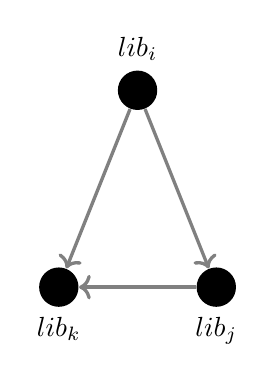
\begin{tikzpicture}[
         roundnode/.style={circle, fill=black, minimum size=5mm},
        squarenode/.style={fill=black, text=red, minimum size=5mm},
     ]
    \begin{scope}
         \node[roundnode, label=above:$lib_i$] (s2_proji) at (3, 2.5) {};
        \node[roundnode, label=below:$lib_j$] (s2_projj) at (4,0) {};
         \node[roundnode, label=below:$lib_k$] (s2_projk) at (2,0) {};
     \end{scope}

     \begin{scope} [every edge/.style={draw=gray, very thick}]
         \path [->] (s2_proji) edge (s2_projj);
         \path [->] (s2_proji) edge (s2_projk);
         \path [->] (s2_projj) edge (s2_projk);
     \end{scope}
     \end{tikzpicture}
    
     \caption{Example dependency graph for a given time period}
     \label{fig:lib}
     \vspace{2ex}
 \end{figure}
\begin{figure}[t]
    \centering

    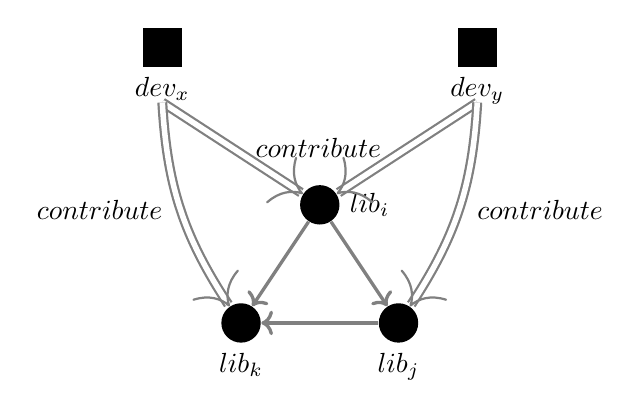
\begin{tikzpicture}[
        roundnode/.style={circle, fill=black, minimum size=5mm},
        squarenode/.style={fill=black, text=red, minimum size=5mm},
    ]
    \begin{scope}
        
        \node[roundnode, label=right:$lib_i$] (s2_proji) at (4, 1.5) {};
        \node[roundnode, label=below:$lib_j$] (s2_projj) at (5,0) {};
        \node[roundnode, label=below:$lib_k$] (s2_projk) at (3,0) {};
        
        \node[squarenode, label=below:$dev_x$] (s3_devx) at (2, 3.5) {};
        
        \node[squarenode, label=below:$dev_y$] (s3_devy) at (6, 3.5) {};
        
    \end{scope}

    \begin{scope} [every edge/.style={draw=gray, very thick}]
        \path [->] (s2_proji)  edge  (s2_projj);
        \path [->] (s2_proji) edge (s2_projk);
        \path [->] (s2_projj) edge (s2_projk);
        
    \end{scope}
    \begin{scope} [every edge/.style={draw=gray, thick, double distance=2pt}]
        \path [->] (6, 2.8) edge node[left = 2mm] {$contribute$} (s2_proji);
        \path [->] (6, 2.8) edge[bend left=15] node[right = 1mm] {$contribute$} (s2_projj);
        \path [->] (2, 2.8) edge node[right = 2mm] {$$} (s2_proji);
        \path [->] (2, 2.8) edge[bend right=15] node[left = 1mm] {$contribute$} (s2_projk);
    \end{scope}
    \end{tikzpicture}
\end{figure}
\begin{figure}[t]
    \centering
    \begin{tikzpicture}[
        roundnode/.style={circle, fill=black, minimum size=5mm},
        squarenode/.style={fill=black, text=red, minimum size=5mm},
    ]
    \end{tikzpicture}
\caption{Example Dependency-Contribution graph showing relationships between contributions and dependencies}
 \label{fig:dc-graph}
\end{figure}

This is just one example of the type of research that is enabled by access to heterogeneous data related to software package ecosystems.

\smallskip\noindent\textbf{Peril 1.}\textit{
 Developers might use different identifiers when contributing to different parts of a software package ecosystem, e.g., when contributing to different libraries.}\\
 
When modelling using such graphs, there is a threat that contributors may use multiple identifiers (i.e., $c_x$ and $c_y$ are the same contributor).
This is a well-known research problem, and there has been work to merge these accounts, such as \cite{wiese2016mailing}.
GitHub has introduced mechanisms such as two-factor authentication\footnote{\url{https://docs.github.com/en/authentication/securing-your-account-with-two-factor-authentication-2fa/configuring-two-factor-authentication}} to counteract the issue of multiple identifiers.
This is since developers might be less likely to switch accounts if it requires cumbersome authentication.


\smallskip\noindent\textbf{Peril 2.}\textit{
Developers' contributions to software package ecosystems might be interspersed with bot contributions, e.g., automated dependency updates.}\\

The rise of automation and artificial intelligence has led to much work on the integration of automated scheduling (i.e., bots) into software development workflows \cite{Storey2016, Farooq2016, Wessel2018, Erlenhov2019, bot_modify_wf} to name a few. These bots are designed to perform specific tasks within a software package ecosystem. For example, a bot may be programmed to automatically update dependencies, test code changes, or deploy software to production. As an example, the Google APIs repo-automation-bots project lists bots for automated labelling of issues and pull requests, automated approval of pull requests, and triggering releases.\footnote{\url{https://github.com/googleapis/repo-automation-bots}}
Bots perform common maintenance tasks in many software projects and are now commonplace \cite{Beschastnikh2017, Urli2018,BIMAN,bot_or_not}.
Especially with bots such as dependabot (automated pull requests to update configurations to reduce the risk of vulnerability threats),\footnote{\url{https://github.com/dependabot}} more and more automation has caused a lot of noise in the contributions between projects.
There are also bots for communication and documentation \cite{Urli2018, Lin2016, Lebeuf2017a}.

To be able to draw accurate conclusions about what humans are doing in software package ecosystems, researchers should consider distinguishing between bot and human contributions.
It is also important to differentiate this from other contributions \cite{maeprasart2022understanding}.
The research community has responded well, with a wide range of techniques and tools to mitigate this peril \cite{Bodegha2021, golzadeh2022accuracy}.

\smallskip\noindent\textbf{Peril 3.}\textit{
Not all developer activities in software package ecosystems are accessible to the public, e.g., library use in proprietary settings.
}\\

Not all developer activities in software package ecosystems are accessible to the public, e.g., when the boundary between open source and industry is blurred \cite{stol2014inner}, which presents a challenge for researchers who aim to study the development process. This is particularly true in proprietary settings where software development is performed behind closed doors or is open source for a limited time period, thus resulting in the artefacts not permanently being publicly available.
This can make it difficult to understand the broader ecosystem in which a software project is developed.
Proprietary settings may lead to non-standardisation in software development practises. Different software projects may use different management systems and tools, making it difficult to accurately compare and analyse software development activities across various projects. For example, some projects may use communication, documentation, and other management tools not captured on the same platform \cite{montgomery2022alternative}. For example, some projects might use Bugzilla instead of issues and pull requests for their bug and code review systems, while others may use Discord, Slack channels, or email threads for their communication needs.

This lack of standardisation in software development practises presents a challenge for researchers who study the software package ecosystem and understand the development process. To address this issue, researchers should strive to collect data from a diverse set of projects to gain a comprehensive understanding of the software package ecosystem. In addition, researchers may need to adjust their methodologies or data collection techniques to accommodate the different tools and practises used by different software projects.

\subsection{Defining Components and their Dependencies}

\smallskip\noindent\textbf{Promise 2.}\textit{
Researchers can access a software package ecosystem's dependency network through package managers and registries, e.g., npm lists the dependencies and dependents for over a million libraries.}\\


With the rise of curated datasets like libraries.io, researchers can now recover and model dependency relations between software units using pre-extracted datasets.
Table \ref{tab:PM_features} shows examples of popular package managers mined from the libraries.io dataset in 2020. 

\begin{table*}[]
\caption{Summary of 13 package managers from libraries.io as ranked by TIOBE in 2020}
 \label{tab:PM_features}
 \centering
\begin{tabular}{@{}llrlll@{}}
\toprule
\begin{tabular}[c]{@{}l@{}}Package \\ Ecosystem\end{tabular} & \begin{tabular}[c]{@{}l@{}}Programming \\ Language\end{tabular} &  \begin{tabular}[c]{@{}l@{}}Tiobe \\ Rank\end{tabular} & Environment & \begin{tabular}[c]{@{}l@{}}Dependency \\ Tree\end{tabular} & \begin{tabular}[c]{@{}l@{}}Package   \\Archive link\end{tabular}\\ \midrule
PyPI & Python & 2 & Python & Flat & pypi.org  \\
Maven & Java & 3 & JVM & Flat & Maven.org  \\
Bower & JavaScript & 7 & Node.js & Flat & bower.io  \\
Meteor & JavaScript & 7 & Node.js & Nested & atmospherejs.com \\
npm & JavaScript & 7 & Node.js & Nested (v2) & npmjs.com  \\
Packagist & PHP & 8 & PHP & Flat & packagist.org \\
Puppet & Ruby & 13 & Ruby MRI & Flat & forge.puppet.com  \\
RubyGems & Ruby & 13 & Ruby MRI & Flat & rubygems.org  \\
CRAN & R & 14 & RStudio & Flat & cran.r-project.org  \\
CPAN & Perl & 15 & Perl & Flat & metacpan.org  \\
GO & Golang & 20 & Go & Flat & pkg.go.dev  \\
NuGet & C\#, VB & 5, 6 & .NET & Flat & nuget.org \\
Anaconda & Python, R, C\# & 2, 14, 5 & Anaconda & Flat & anaconda.org  \\ \bottomrule
\end{tabular}
\end{table*}

\smallskip\noindent\textbf{Peril 4.}\textit{
Different software package ecosystems define the concept of ``dependency'' differently, e.g., by allowing or not allowing different versions of a library on the same dependency tree.
}\\

Different software package ecosystems have varying definitions of what constitutes a dependency. For example, some ecosystems may allow multiple versions of a library to exist on the same dependency tree, while others may restrict developers to a single version of a library \cite{Islam}. These restrictions are often based on the programming language being used, as different languages have different approaches to managing dependencies. It is important to consider the restrictions on dependency relationships when studying software package ecosystems, as they can have a major impact on the development process. For example, the ability to use multiple versions of a library on the same dependency tree can greatly simplify the process of updating dependencies and can make it easier to resolve conflicts between libraries.

One way to visualise the impact of these restrictions is to compare the difference between a nested dependency tree and a directed dependency tree, as shown in Figure \ref{fig:nest}.\footnote{Taken from \url{https://npm.github.io/how-npm-works-docs/npm3/how-npm3-works.html}} This distinction is important because it highlights the different ways that a software unit can depend on different versions of the same library.
In this example, npm v3 creates the dependency tree based on the installation order, therefore flattening unnecessary nested dependencies (i.e., B v1.0 in cyan). This reduces the complexity of a nested tree by resolving some of the transitive dependencies (nested dependencies).

\begin{figure}
	\centering
	\includegraphics[width=.8\textwidth]{book/chapter-promisesandperils/pics/nestedv2.jpg}
	\caption{Difference between flat and nested dependencies}
	\label{fig:nest}
\end{figure}

\smallskip\noindent\textbf{Peril 5.}\textit{
Developers might declare a dependency to other parts of a software package ecosystem but not use it, e.g., because they failed to update its removal.
}\\

It is common for developers to declare dependencies on other parts of the software package ecosystem but not always use them. This can happen for various reasons, such as forgetting to remove the dependency after it is no longer needed. This can pose a challenge for researchers who are trying to extract dependencies from package managers, like those in configuration files, as there may be inconsistencies between the listed dependencies and what is actually being compiled and used by the code. This can lead to a biased understanding of the software package ecosystem and the relationships between software components.

To address this issue, there have been numerous efforts to track the actual library dependencies compiled and executed in software systems. These efforts aim to provide a more accurate understanding of the dependencies and the relationships between software components. For example, research has been conducted on the use of dynamic analysis to track compiled dependencies in real time and on the development of tools to automatically detect and track executed dependencies \cite{Zapata:ICSME2018, Ponta2018,Chinthanet:ASE2020}.

\subsection{Defining Boundaries and Completeness}

\smallskip\noindent\textbf{Promise 3.}\textit{
Researchers can use the boundaries of software package ecosystems to study communities of developers, e.g., developers contributing to and/or benefiting from the npm ecosystem.
}\\

Following Promise 2, the emergence of package managers has also led to studies that approximate software communities.
Using the libraries.io dataset, researchers were able to study projects that host libraries that use package managers.
Researchers have used this dataset to compare different library ecosystems \cite{kikas.2017,decan:emse:2019,CogoDown2019}.


\smallskip\noindent\textbf{Peril 6.}\textit{
Package managers do not always represent software package ecosystems, their communities, or their sub-communities, e.g., in cases where multiple package managers exist.
}\\

Package managers are a fundamental aspect of software package ecosystems, but do not always fully represent the complex relationships and interactions that occur within a community of developers and users, as shown in Table~\ref{tab:PM_features}. In some cases, multiple package managers exist for the same programming language, creating a complex landscape of software libraries and dependencies that are not always easily understood. For instance, Bower and Meteor manage npm libraries, which can lead to confusion and overlap in the management of dependencies.

Similarly, Java, Scala, Android, and other Java-based open source communities all use the Maven package manager, but each of these communities has its own unique set of libraries, dependencies, and development practises. Researchers should be aware of the limitations of package managers when studying software package ecosystems, and consider the broader context and relationships that exist within these communities. 

\smallskip\noindent\textbf{Peril 7.}\textit{
Lack of activity in parts of a software package ecosystem does not necessarily indicate project failure, e.g., when highly depended-upon libraries are feature-complete.
}\\

It is important to note that lack of activity in a part of a software package ecosystem does not always mean project failure \cite{coelho2017modern}. In some cases, highly relied-upon libraries that have reached feature-completeness may see little activity, but continue to be used by the software community. 

However, it is still important to consider the long-term sustainability of these libraries, especially given the rate at which technology and software development practises change. This has become a topic of interest in recent years, and researchers have explored best practises for sustaining open source projects and ensuring their continued success \cite{Ait2022,valiev2018ecosystem}. Understanding the factors that contribute to project sustainability is important to ensure the longevity and continued growth of software package ecosystems.

\smallskip\noindent\textbf{Peril 8.}\textit{
Sampling from a software package ecosystem is challenging since sub-setting might alter the dependency network, e.g., by breaking dependency chains.
}\\

Sampling from a package ecosystem is not straightforward, as the sample composition can be significantly affected due to missing dependency links between libraries. For instance, a subset of the ecosystem might alter the dependencies between libraries, leading to the breakdown of the dependency chains. This could lead to an incomplete picture of the software package ecosystem, leading to incorrect conclusions from a study. To minimise this risk, researchers should carefully consider the boundaries of their study and choose the appropriate sampling method based on the research questions and goals. For example, researchers could focus on popular, highly dependent, or risk-vulnerable aspects of the ecosystem as a starting point. 
For some ecosystems, the number of downloads, GitHub stars, and watchers are other aspects for the researcher to utilise.


\smallskip\noindent\textbf{Peril 9.}\textit{
Sampling from a software package ecosystem is challenging since the dependency network changes over time, e.g., when dependencies are added, removed, upgraded, or downgraded.
}\\

The dynamic nature of package ecosystems and the constant changes to their dependencies can impact the generalisability of the results. Therefore, it is important to also consider the time granularity of the analysis. For example, if the goal is to understand the evolution of dependencies over time, a finer time granularity may be necessary to capture the smaller changes and trends. However, if the goal is to understand the overall structure and relationships within the ecosystem, a coarser time granularity may be sufficient. Based on recent studies \cite{wattanakriengkrai2022giving,valiev2018ecosystem,Mirsaeedi:icse2020, Brindescu:emse2020, Nassif:icsme2017}, a three-month window seems appropriate for some studies.
Another level of granularity to consider is the size of the component. For instance, there are cases where a single package may contain more than one repository, especially for large library frameworks. 
The granularity also depends on the nature of the ecosystem itself. For instance, researchers should understand whether the ecosystem comprises library packages (e.g., PyPI), plugins (e.g., Eclipse), or is a library distribution (e.g., Android).



\subsection{Analysing and Visualising the Data}

\textbf{Peril 10.}\textit{
Analysing and visualising entire software package ecosystems is challenging due to their size, e.g., in terms of nodes and edges in the network.
}\\

The size of software package ecosystems implies large data sets, which can be overwhelming for tools and algorithms to analyse and display. Therefore, it may be necessary to make choices about the granularity of the data included in the analysis and visualisation. Another alternative is to focus on the most critical parts of the software package ecosystem, such as the high-level structure, highly dependent packages, or parts of the system that pose a risk to security and reliability. 
The key is to strike a balance between detail and simplicity, providing a meaningful representation of the ecosystem while being able to handle the complexity of its size.


\section{Application: When to Apply Which Peril}
\label{PPM:sec:application}

We include a disclaimer stating that not all perils are applicable to every mining situation. To demonstrate the practical application of our perils and their mitigation, we present two case studies that involve mining the software package ecosystem. Each case study has a distinct research objective and focusses on a specific dataset to be mined.

\subsection{Two Case Studies}
Table \ref{tab:cases} presents the two case studies we have selected for this analysis.
The \textit{first case} involves mining for contributions congruent to dependency updates \cite{wattanakriengkrai2022giving}. 
In this work, the authors mine GitHub repositories for Pull Requests and Issues that were submitted and merged congruent to dependency updates within the npm ecosystem. 
The \textit{second case} involves mining communication data for the Eclipse ecosystem \cite{Nugroho2021}. Although the second case does not mine for dependency relations (i.e., use relations),  we show that these perils still apply when mining for other relationships in an ecosystem.
Moreover, the second case studies the Eclipse ecosystem, which is a different dataset compared to the more popular GitHub dataset.

\subsection{Applying Perils and their Mitigation Strategies}
Table \ref{tab:perilsapp} provides a summary of the perils that can be applied to each of the case studies. We will now go into the details of mitigation strategies based on these perils. 
For better organisation and understanding, we have grouped the perils according to the four logical processes for mining.

\smallskip\noindent\textbf{Information to Mine}. 
The first set of mitigation strategies, which addresses perils 1-3, focusses on planning which information to mine. There are two primary strategies that researchers can employ:


\begin{enumerate}
    \item Researchers should use research tools and techniques to remove noise and other biases in the dataset, such as bot detection and the handling of multiple identities. This strategy was implemented in both case studies, as contributions and discussions often have the potential to involve bots or developers with multiple identities.
\item Depending on the research goals, researchers should recognise that not all contributions are equal and filter the dataset accordingly.
\end{enumerate}

We applied these two strategies to both cases. In the first case, the goal was to capture all congruent contributions, so we filtered out contributions made to libraries without dependencies. Since all npm packages are listed in the registry, Peril 3 (private activities) did not apply.
In the second case, we addressed Peril 1 by conducting a qualitative analysis to ensure that the member identities were not duplicated, as Eclipse developers were known to change identities. To mitigate Peril 2, we removed bot responses. For the second case, since all forum data is made public, Peril 3 did not apply.


\begin{table}
\centering
\caption{Description of the research objectives and datasets for the case studies}
 \label{tab:cases}
\begin{tabular}{lp{5cm}r} 
\toprule
\textbf{Case Study} & \textbf{Research Objective}                                                          & \textbf{Datasets}           \\
\midrule
Wattanakriengkrai \etal \cite{wattanakriengkrai2022giving}             & Explore code contributions between library and client (i.e, use-relations)  & libraries.io\\
& &  GitHub API \\
Nugroho \etal \cite{Nugroho2021}                & Explore discussion contributions between contributors (i.e., contributions) & Eclipse API                \\
\bottomrule
\end{tabular}
\end{table}

\begin{table}
\centering
\caption{Application of each peril to the case studies}
 \label{tab:perilsapp}
\begin{tabular}{rp{8cm}ccc} 
\toprule                   
& \textbf{Perils}       & case 1      & case 2                 \\
                                                                               & & npm  & Eclipse   \\
\midrule
\textbf{P1} &Developers might use different identifiers when contributing to different parts of a software package ecosystem, e.g., when contributing to different libraries.                             &    \CheckedBox         &          \CheckedBox           \\ 
%\hline
\textbf{P2} & Developers' contributions to software package ecosystems might be interspersed with bot contributions, e.g., automated dependency updates.                                                      &      \CheckedBox               &      \CheckedBox               \\ 
%\hline
\textbf{P3} & Not all developer activities in software package ecosystems are accessible to the public, e.g., library use in proprietary settings.                                                         &         -           &      \CheckedBox               \\ 
%\hline
\textbf{P4} & Different software package ecosystems define the concept of \`{}\`{}dependency'' differently, e.g., by allowing or not allowing different versions of a library on the same dependency tree. &         \CheckedBox       &     -                            \\ 
%\hline
\textbf{P5} & Developers might declare a dependency to other parts of a software package ecosystem but not use it, e.g., because they failed to update its removal.                                        &     -           &  -    \\
%\hline
\textbf{P6} &Package managers do not always represent software package ecosystems, their communities, or their sub-communities, e.g., in cases where multiple package managers exist.                     &     -                   &  -                  \\
%\hline
\textbf{P7} & Lack of activity in parts of a software package ecosystem does not necessarily indicate project failure, e.g., when highly depended-upon libraries are feature-complete.                     &       \CheckedBox         &  -                           \\
%\hline
\textbf{P8} &Sampling from a software package ecosystem is challenging since sub-setting might alter the dependency network, e.g., by breaking dependency chains.                                         &        \CheckedBox        &     \CheckedBox                                \\
%\hline
\textbf{P9} &Sampling from a software package ecosystem is challenging since the dependency network changes over time, e.g., when dependencies are added, removed, upgraded, or downgraded.               &       \CheckedBox         &     -                          \\
%\hline
\textbf{P10} &Analysing and visualising entire software package ecosystems is challenging due to their size, e.g., in terms of nodes and edges in the network.                                  &        \CheckedBox      &      \CheckedBox               \\
\bottomrule
\end{tabular}
\end{table}

\smallskip\noindent\textbf{Defining Dependencies}. 
The second set of perils (Perils 4-5) is related to dependency relationships between software units, and only the first case study is applicable. To address these perils, researchers should adopt the following strategy:

\begin{enumerate}
    \item Researchers should not rely solely on listed dependencies in configuration files (e.g., pom.xml, package.json, etc.) as a measure of dependency between two components. Instead, code-centric approaches should be used to validate which libraries are actually depended upon.
\end{enumerate}

For example, in the first case, in addition to mining the configuration information, the authors also analysed the similarity of the source code contributions to address Peril 4. Regarding Peril 5, since the study's objective was to investigate changes to the configuration files, the risk of the update not being executed was deemed less important.
It is important to note that the second case study did not include dependency analysis and, therefore, these perils did not apply.

\begin{figure*}[]
    \centering
    \begin{subfigure}{0.9\linewidth}
         \includegraphics[width=1.1\textwidth]{book/chapter-promisesandperils/pics/congruentViz.jpg}
         \caption{Visualization of a Time analysis for 107,242 libraries.}
     \end{subfigure}
     \begin{subfigure}{0.9\linewidth}
         \includegraphics[width=1\textwidth]{book/chapter-promisesandperils/pics/eclipseViz.jpg}
         \caption{A Visual Topology map for 832,058 threads}
     \end{subfigure}
    \caption{Visualisation examples for the two case studies}
    \label{fig:visCase}
\end{figure*}

\smallskip\noindent\textbf{Defining Boundaries}.
The third set of perils (Perils 6-9) is related to the definition of boundaries and completeness and is relevant for both case studies. To mitigate these perils, we recommend the following strategies:

\begin{enumerate}
    \item Researchers should recognise that a dormant project does not necessarily mean that it is inactive. Instead, studies can use alternative heuristics, such as the number of dependents and dependencies, as better indicators of a project's importance in the ecosystem.
    \item Researchers should not rely solely on the programming language to define sub-communities. Using a common package manager for the programming language is a more effective rule of thumb for distinguishing boundaries.
    \item Researchers should avoid random sampling. Instead, sampling should be tailored to the research goals by considering factors such as an appropriate time window or focussing on specific attributes of components (e.g., most dependents, most popular, most contributors).
\end{enumerate}


Peril 6 did not apply to any of the case studies. 
Particularly for the first case, since the goal was to explore the npm package ecosystem, we assumed that the boundaries were clearly defined by the npm registry. 
Similarly, the second case study used the generic Eclipse platform as the boundary. 
Peril 7 was applied to the npm study, while Peril 8 was applied to both case studies. 
As a result, the two cases conducted a qualitative analysis of the dataset to gain deeper insights.
In the first case study, a three-month time window was created to capture dependencies. 
For the second case study, forum contributors were sampled into three groups (i.e., junior, member, or senior) according to the sliding window of their contributions. 

\smallskip\noindent\textbf{Visualisation}.
The final peril (Peril 10) relates to visualisation, which can be challenging due to the vast size and complexity of software ecosystems. As it is not feasible to visualise every aspect of an ecosystem simultaneously, a focused approach is necessary. A mitigation strategy is to select specific attributes of the ecosystem (e.g., the most dependent, most popular, and most contributions) that align with the research needs and objectives. 

Figure \ref{fig:visCase} shows two cases where visualizations are employed to gain insights, especially for large datasets.
In the first figure (a), we visualize the distributions of the data set and applied the appropriate statistical tests, along with the effect size, to test our hypotheses and answer research questions. 
In the second example (b), although not directly related to package ecosystems, the authors utilized a topological visualization \cite{Lum2013ExtractingIF} to gain insights on the over 800,000 forum threads of discussions. 



\section{Chapter Summary}
In this chapter, we explore the various aspects of mining information from the software package ecosystem, presenting three promises and ten perils that researchers should be aware of when undertaking such tasks. The chapter is structured around four key processes for mining: 1) Planning what Information to Mine, 2) Defining Components and their Dependencies, 3) Defining Boundaries and Completeness, and 4) Analysing and Visualising the Data. To help new and experienced researchers navigate these challenges, we introduced the SUG model, which can serve as a valuable tool to minimise threats to validity. Although some perils may be more relevant to specific research objectives, our aim is to equip researchers with the knowledge and resources needed to confidently gather and integrate software package ecosystem data into their work.
%The Software Heritage Research and Open Science Ecosystem
% %Semantic labeling three-letter-code: SWH (e.g. \chapter{SWH})


\title{Promises and Perils of Mining \\ Software Package Ecosystem Data}
\author{Raula Gaikovina Kula \and Katsuro Inoue \and Christoph Treude}
\institute{Raula Gaikovina Kula \at Nara Institute of Science and Technology, Japan, \email{raula-k@naist.jp}
\and Katsuro Inoue \at Nanzan University, Japan \email{ inoue599@nanzan-u.ac.jp}
\and  Christoph Treude \at The University of Melbourne, Australia \email{christoph.treude@unimelb.edu.au}}

\maketitle
\label{PPM:ch}
\abstract*{The use of third-party packages is becoming increasingly popular and has led to the emergence of large software package ecosystems with a maze of inter-dependencies. Since the reliance on these ecosystems enables developers to reduce development effort and increase productivity, it has attracted the interest of researchers: understanding the infrastructure and dynamics of package ecosystems has given rise to approaches for better code reuse, automated updates, and the avoidance of vulnerabilities, to name a few examples. But the reality of these ecosystems also poses challenges to software engineering researchers, such as: How do we obtain the complete network of dependencies along with the corresponding versioning information? What are the boundaries of these package ecosystem? How do we consistently detect dependencies that are declared but not used? How do we consistently identify developers within a package ecosystem? How much of the ecosystem do we need to understand to analyse a single component? How well do our approaches generalise across different programming languages and package ecosystems? In this chapter, we review promises and perils of mining the rich data related to software package ecosystems available to software engineering researchers.}

\abstract{The use of third-party packages is becoming increasingly popular and has led to the emergence of large software package ecosystems with a maze of inter-dependencies. Since the reliance on these ecosystems enables developers to reduce development effort and increase productivity, it has attracted the interest of researchers: understanding the infrastructure and dynamics of package ecosystems has given rise to approaches for better code reuse, automated updates, and the avoidance of vulnerabilities, to name a few examples. But the reality of these ecosystems also poses challenges to software engineering researchers, such as: How do we obtain the complete network of dependencies along with the corresponding versioning information? What are the boundaries of these package ecosystems? How do we consistently detect dependencies that are declared but not used? How do we consistently identify developers within a package ecosystem? How much of the ecosystem do we need to understand to analyse a single component? How well do our approaches generalise across different programming languages and package ecosystems? In this chapter, we review promises and perils of mining the rich data related to software package ecosystems available to software engineering researchers.}

%%%%%%%%%%%%%%%%%%%%%%%%%%%%%%%%%%%%%%%%%%%%%%%%%%%%%%%%%%%%%%%%%%

\section{Introduction}
\label{PPM:sec:definition}

Third-party libraries are a great way for developers to incorporate code without having to write their own for every functionality required. By using these libraries, developers can save time and energy while still getting the functions they need.
Using third-party libraries is becoming increasingly popular and has led to the emergence of large software package ecosystems such as npm. While these ecosystems offer many benefits, they also come with risks, such as software vulnerability attacks \cite{Chinthanet:ASE2020}.

Large software package ecosystems are a treasure trove for researchers who can investigate a wide range of questions. For example, by studying activity in large ecosystems, researchers can identify which libraries are the most popular and learn what characteristics make them successful \cite{kikas.2017,decan:emse:2019}.
Additionally, research on large ecosystems can help developers understand how to protect their code from malicious actors who may attempt to exploit vulnerabilities or insert malware into popular libraries.
Studying large software package ecosystems can help us better understand the dynamics of open source development in general. Open source development is a complex process that involves many different stakeholders working together (or sometimes competing) to create valuable code that anyone can use or improve upon. By understanding how these interactions play out in different types of ecosystem structures -- including those with many small projects versus few very large ones -- we can develop insights that might be applicable more broadly across other types of collaborative systems.

In this chapter, we identify and discuss promises and perils during the mining process, ranging from planning what information to mine from the ecosystem to analysing and visualising the mined data. 
Therefore, the chapter is broken down into these logical processes of mining ecosystem data: 1) Planning what Information to Mine, 2) Defining Components and their Dependencies, 3) Defining Boundaries and Completeness, and 4) Analysing and Visualising the Data.

This chapter is intended for researchers and practitioners who are interested in exploring and exploiting software package ecosystem information from a diverse range of sources that are publicly available. 
We also highlight the pitfalls to consider during the mining process, particularly when these pitfalls could lead to a misinterpretation of the analysis and results. 
The chapter is written in a manner that encourages newcomers who have little or no experience or who are interested in utilising ecosystem data across different disciplines outside of software engineering.
Our goal is to get new researchers quickly accustomed to gathering ecosystem information for their research.


\section{A Component-based Software Ecosystem}

Defined as a component-based software ecosystem, we suggest using the term `software package ecosystem' as a suitable term for the symbiotic relationships among third-party library components (as software projects or repositories), as these libraries and their dependent clients coexist on the same technological platform, therefore sharing the same environment and other internal and external factors (e.g., security threats, sharing contributions, etc.).
Please refer to the Introduction chapter for an in-depth definition of the different types of software ecosystems.
We present our interpretation of the software package ecosystem in Kula et al.~\cite{KulaSANER18}, where we formally define a package ecosystem using a Software Universe Graph (SUG).
This is modelled as a structured abstraction of the evolution of software systems and their library dependencies over time.

%%%%%%%%%%%%%%%%%%%%%%%%%%%%%%%%%%%%%%%%%%
\begin{figure*}
	\centering
	\includegraphics[width=.7\textwidth]{book/chapter-promisesandperils/pics/UniversalExample.jpg}
	\caption{Conceptual example of the Software Universe Graph, depicting the use and update relationships between different software units.}
	\label{fig:SUG}
\end{figure*}
%%%%%%%%%%%%%%%%%%%%%%%%%%%%%%%%%%%%%%%%%%%%%


\paragraph{\textbf{Component-based Representation as a Software Universe Graph}}
\label{PPM:sec:SUG}

First introduced by Kula et al.~\cite{KulaSANER18}, the \textit{Software Universe Graph} (SUG) is a structural abstraction of the software ecosystem of third-party libraries.
Figure \ref{fig:SUG} provides an illustration of the different relationships within the graph.
Let $G= (N,E)$ represent a graph $G$. $N$ is a set of nodes, each node representing a software unit. 
We define a software unit as a version instance of any software program. 

The authors then present the \textit{use} and \textit{update} relationships that exist in the ecosystem.
Hence, the edges $E$ are composed of $E_{use}$ and $E_{update}$. $E_{use}$ is a set of \textit{use-relations} and $E_{update}$ is a set of \textit{update-relations}.

\begin{definition}
An edge $u \rightarrow v \in E_{use}$ means that $u$ uses $v$. The defined functions of $E_{use}$ are:

\begin{equation}
\small
\small \use(u)\equiv \{v|u \rightarrow v\}
\normalsize
\end{equation}
\begin{equation}
\small
\small \useBy(u)\equiv \{v|v \rightarrow u\}
\normalsize
\end{equation}
\end{definition}

Use-relations can be extracted from either the source code or configuration files. 
As shown in Figure \ref{fig:SUG}, node $a1$ uses node $x1$. 
In addition, node $x1$ is used by nodes $a1$, $q1$, and $q2$. Parallel edges for node pairs are not allowed.

\begin{definition}
We represent an update relation from node $a$ to $b$ using $ a \Rightarrow b $, which means that the newer update $b$ was released from node $a$ and is defined as:
\begin{equation}
\small a \Rightarrow b \in E_{update}
\end{equation}
\end{definition}

Update relations refer to when a successive release of a software unit is made available. Figure \ref{fig:SUG} shows that node $q1$ is first updated to node $q2$. Later, node $q2$ is updated to the latest node $q3$. Hence, $q1 \Rightarrow q2 \Rightarrow q3$.
Note that an update should not be confused with forking. 
We distinguish a fork as a separate software unit. 
Each node in the SUG should be denoted by three attributes: \texttt{<name,release,time>}.  
For a node $u$, we define:

\begin{itemize}
	\item \textbf{u.name} Name is the string representation identifier of a software unit.
	We introduce the name axiom: For nodes $u$ and $v$, if $u \Rightarrow v$, then $u.name = v.name$ holds.
	
	\item \textbf{u.release}. Release refers to the specific assigned change reference for a software unit. For nodes $u$ and $v$, if $u \Rightarrow v$
	then $v$ is the immediate successor of $u$. Note that the versioning pattern may vary from project to project. 
	\item \textbf{u.time}. Time refers to the time stamp at which node $u$ was released. For nodes $u$ and $v$ of $u \Rightarrow v$, $u.time < v.time$.
\end{itemize}

\begin{figure}
	\centering
	\includegraphics[width=.8\textwidth]{book/chapter-promisesandperils/pics/TemporalSUG.jpg}
	\caption{Temporal property of the SUG}
	\label{fig:SUGTemp}
\end{figure}

\begin{definition}
    
	The SUG has temporal properties.
This describes the simultaneity or ordering in reference to time. Let SUG $G = (N, E) $ be at time $t$. At time $t^{\prime} > t$, we observe an extension of $G$, such that:

\begin{equation}
\small G^{\prime} = (N \cup \Delta N, E \cup \Delta E)
\end{equation}
where $\Delta E \cap (N \times N) = \emptyset$
\end{definition}

Figure \ref{fig:SUGTemp} illustrates the temporal properties of the SUG. 
Here, it is observed that $G'$ is composed of $G$ augmented with newly added node $a3$ and its corresponding $a3 \rightarrow x2$ and $a2 \Rightarrow a3$ relations.
A SUG grows monotonically over time with only additions.
Here, we consider that modification or deletion changes on the SUG do not occur. 

\begin{definition}
    A timed SUG specifies the state of the SUG at any point in time.
So for an SUG $G=(N,E)$, we represent a timed SUG $G_{t}$ at time $t$ as a sub-graph of $G$. Formally,
\begin{equation}
\small G_t\equiv(N_{t}, E_{t})
\end{equation}
where $N_{t} = \{u|u \in N, u.time \leq t \}$ and $E_t = \{ e | e \in E \wedge e \in  N_t \}$
\end{definition}
	


\section{Data Sources}
Researchers can use various datasets to model the ecosystem using the SUG model of usage and update relationships.
The most obvious data source that has revolutionised data mining in the software engineering domain is the GitHub platform. 
Established in 2008, and then purchased by Microsoft in 2020, GitHub is home to various popular Open Source Software. 
GitHub is built on the git version control system and is useful for storing all changes made to a repository. 
In the case of the SUG, a GitHub repository can represent one software unit, whose depend relations can be extracted via a configuration file (such as the package.json file for JavaScript projects).
The repository should also contain the release information that holds the update relations.
Due to its large size, researchers and the GitHub team have made available datasets for researchers to mine, for example through the GitHub API/Graph QL.\footnote{\url{https://docs.github.com/en/graphql}} This is the backend Application Programming Interface (API) that can be used to query large amounts of data on GitHub. Most researchers use the API to download and mine information from the GitHub platform. 
It is important to note that while GitHub introduced a new feature of Dependency Graphs to map the depend relationship,\footnote{\url{https://docs.github.com/en/code-security/supply-chain-security/understanding-your-software-supply-chain/about-the-dependency-graph}} most older projects do not have this feature.
In this case, the researcher would need to manually extract and query the configuration files for dependency information. 

We refer to the first chapter for additional information on data sources for mining software ecosystems. 

\section{Promises and Perils}
\label{PPM:sec:promisesperils}

Using the SUG model of depend and use relations and the available datasets, we can now present our promises and perils of mining ecosystem information.

\subsection{Planning What Information to Mine}

\textbf{Promise 1.}\textit{
Researchers can access and link heterogeneous data related to software package ecosystems, e.g., package registries and bug trackers.}\\

When planning what information to mine from the ecosystem, researchers do not need to limit themselves to the usage and update relationship information.
Platforms that host software repositories include other software management systems such as bug trackers.
For example, GitHub allows researchers to manage GitHub Pull Requests, Issues, and Discussions not only for one project, but for multiple projects.
GitHub provides three management systems that are related to a software repository:

\begin{itemize}
    \item \textit{GitHub Discussions}\footnote{\url{https://docs.github.com/en/discussions}} - The GitHub Discussions forum is a collaborative communication forum for the community around an open source or internal project. Community members can ask and answer questions, share updates, have open-ended conversations, and follow along on decisions affecting the community's way of working.
    \item \textit{GitHub Pull Requests}\footnote{\url{https://docs.github.com/en/pull-requests}} - Pull Requests allow other developers from an ecosystem to make a contribution to a software repository. Pull requests also allow maintainers to discuss and review potential changes with collaborators and add follow-up commits before changes are merged into the software.
    \item \textit{GitHub Issues}\footnote{\url{https://docs.github.com/en/issues}} - Issues are used to track ideas, feedback, tasks, or bugs for work on GitHub.
\end{itemize}

These three systems are examples of how developers contribute to both their own and other projects. 
Hence, to incorporate this information, we can extend the SUG model, creating a model that includes a contribution relationship \cite{wattanakriengkrai2022giving}.

% Note that other platforms may also have management systems, like GitLab, BitBucket and Eclipse.

\begin{definition}
	A Dependency-Contribution graph incorporates contributions by developers whose libraries are involved in dependency relationships. 
\end{definition}

In this work \cite{wattanakriengkrai2022giving}, the authors explore the congruence between dependency updates and developer contributions, based on the original concept of social-technical congruence \cite{stcCataldo2008} where developers contribution patterns are congruent with their coordination needs. Hence, the goal is to identify contributions that are congruent to dependency updates.
As shown in Figure \ref{fig:lib} the authors extend from the typical SUG graph model where $lib_i$ depends (use) on  $lib_k$ and  $lib_j$, while  $lib_j$ also depends on $lib_k$, to the example shown in Figure \ref{fig:dc-graph}.
Different to the SUG, the graph captures developers and their contributions (i.e., the square as $dev_x$ and $dev_y$ represent two different developers making a contribution).
Here contributions are defined as $c$ (Pull Request or Issue) that were submitted to both a library and the client that depends on that library.
Hence, the graph can show contributions that are congruent to dependency changes for a software unit. 

\begin{figure}[t]
     \centering
     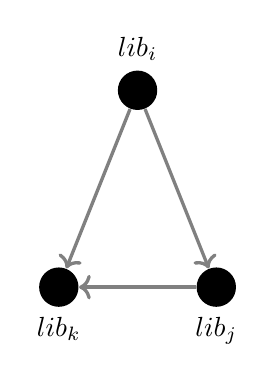
\begin{tikzpicture}[
         roundnode/.style={circle, fill=black, minimum size=5mm},
        squarenode/.style={fill=black, text=red, minimum size=5mm},
     ]
    \begin{scope}
         \node[roundnode, label=above:$lib_i$] (s2_proji) at (3, 2.5) {};
        \node[roundnode, label=below:$lib_j$] (s2_projj) at (4,0) {};
         \node[roundnode, label=below:$lib_k$] (s2_projk) at (2,0) {};
     \end{scope}

     \begin{scope} [every edge/.style={draw=gray, very thick}]
         \path [->] (s2_proji) edge (s2_projj);
         \path [->] (s2_proji) edge (s2_projk);
         \path [->] (s2_projj) edge (s2_projk);
     \end{scope}
     \end{tikzpicture}
    
     \caption{Example dependency graph for a given time period}
     \label{fig:lib}
     \vspace{2ex}
 \end{figure}
\begin{figure}[t]
    \centering

    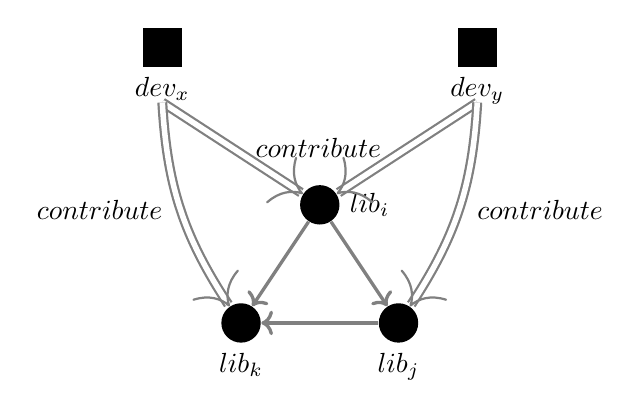
\begin{tikzpicture}[
        roundnode/.style={circle, fill=black, minimum size=5mm},
        squarenode/.style={fill=black, text=red, minimum size=5mm},
    ]
    \begin{scope}
        
        \node[roundnode, label=right:$lib_i$] (s2_proji) at (4, 1.5) {};
        \node[roundnode, label=below:$lib_j$] (s2_projj) at (5,0) {};
        \node[roundnode, label=below:$lib_k$] (s2_projk) at (3,0) {};
        
        \node[squarenode, label=below:$dev_x$] (s3_devx) at (2, 3.5) {};
        
        \node[squarenode, label=below:$dev_y$] (s3_devy) at (6, 3.5) {};
        
    \end{scope}

    \begin{scope} [every edge/.style={draw=gray, very thick}]
        \path [->] (s2_proji)  edge  (s2_projj);
        \path [->] (s2_proji) edge (s2_projk);
        \path [->] (s2_projj) edge (s2_projk);
        
    \end{scope}
    \begin{scope} [every edge/.style={draw=gray, thick, double distance=2pt}]
        \path [->] (6, 2.8) edge node[left = 2mm] {$contribute$} (s2_proji);
        \path [->] (6, 2.8) edge[bend left=15] node[right = 1mm] {$contribute$} (s2_projj);
        \path [->] (2, 2.8) edge node[right = 2mm] {$$} (s2_proji);
        \path [->] (2, 2.8) edge[bend right=15] node[left = 1mm] {$contribute$} (s2_projk);
    \end{scope}
    \end{tikzpicture}
\end{figure}
\begin{figure}[t]
    \centering
    \begin{tikzpicture}[
        roundnode/.style={circle, fill=black, minimum size=5mm},
        squarenode/.style={fill=black, text=red, minimum size=5mm},
    ]
    \end{tikzpicture}
\caption{Example Dependency-Contribution graph showing relationships between contributions and dependencies}
 \label{fig:dc-graph}
\end{figure}

This is just one example of the type of research that is enabled by access to heterogeneous data related to software package ecosystems.

\smallskip\noindent\textbf{Peril 1.}\textit{
 Developers might use different identifiers when contributing to different parts of a software package ecosystem, e.g., when contributing to different libraries.}\\
 
When modelling using such graphs, there is a threat that contributors may use multiple identifiers (i.e., $c_x$ and $c_y$ are the same contributor).
This is a well-known research problem, and there has been work to merge these accounts, such as \cite{wiese2016mailing}.
GitHub has introduced mechanisms such as two-factor authentication\footnote{\url{https://docs.github.com/en/authentication/securing-your-account-with-two-factor-authentication-2fa/configuring-two-factor-authentication}} to counteract the issue of multiple identifiers.
This is since developers might be less likely to switch accounts if it requires cumbersome authentication.


\smallskip\noindent\textbf{Peril 2.}\textit{
Developers' contributions to software package ecosystems might be interspersed with bot contributions, e.g., automated dependency updates.}\\

The rise of automation and artificial intelligence has led to much work on the integration of automated scheduling (i.e., bots) into software development workflows \cite{Storey2016, Farooq2016, Wessel2018, Erlenhov2019, bot_modify_wf} to name a few. These bots are designed to perform specific tasks within a software package ecosystem. For example, a bot may be programmed to automatically update dependencies, test code changes, or deploy software to production. As an example, the Google APIs repo-automation-bots project lists bots for automated labelling of issues and pull requests, automated approval of pull requests, and triggering releases.\footnote{\url{https://github.com/googleapis/repo-automation-bots}}
Bots perform common maintenance tasks in many software projects and are now commonplace \cite{Beschastnikh2017, Urli2018,BIMAN,bot_or_not}.
Especially with bots such as dependabot (automated pull requests to update configurations to reduce the risk of vulnerability threats),\footnote{\url{https://github.com/dependabot}} more and more automation has caused a lot of noise in the contributions between projects.
There are also bots for communication and documentation \cite{Urli2018, Lin2016, Lebeuf2017a}.

To be able to draw accurate conclusions about what humans are doing in software package ecosystems, researchers should consider distinguishing between bot and human contributions.
It is also important to differentiate this from other contributions \cite{maeprasart2022understanding}.
The research community has responded well, with a wide range of techniques and tools to mitigate this peril \cite{Bodegha2021, golzadeh2022accuracy}.

\smallskip\noindent\textbf{Peril 3.}\textit{
Not all developer activities in software package ecosystems are accessible to the public, e.g., library use in proprietary settings.
}\\

Not all developer activities in software package ecosystems are accessible to the public, e.g., when the boundary between open source and industry is blurred \cite{stol2014inner}, which presents a challenge for researchers who aim to study the development process. This is particularly true in proprietary settings where software development is performed behind closed doors or is open source for a limited time period, thus resulting in the artefacts not permanently being publicly available.
This can make it difficult to understand the broader ecosystem in which a software project is developed.
Proprietary settings may lead to non-standardisation in software development practises. Different software projects may use different management systems and tools, making it difficult to accurately compare and analyse software development activities across various projects. For example, some projects may use communication, documentation, and other management tools not captured on the same platform \cite{montgomery2022alternative}. For example, some projects might use Bugzilla instead of issues and pull requests for their bug and code review systems, while others may use Discord, Slack channels, or email threads for their communication needs.

This lack of standardisation in software development practises presents a challenge for researchers who study the software package ecosystem and understand the development process. To address this issue, researchers should strive to collect data from a diverse set of projects to gain a comprehensive understanding of the software package ecosystem. In addition, researchers may need to adjust their methodologies or data collection techniques to accommodate the different tools and practises used by different software projects.

\subsection{Defining Components and their Dependencies}

\smallskip\noindent\textbf{Promise 2.}\textit{
Researchers can access a software package ecosystem's dependency network through package managers and registries, e.g., npm lists the dependencies and dependents for over a million libraries.}\\


With the rise of curated datasets like libraries.io, researchers can now recover and model dependency relations between software units using pre-extracted datasets.
Table \ref{tab:PM_features} shows examples of popular package managers mined from the libraries.io dataset in 2020. 

\begin{table*}[]
\caption{Summary of 13 package managers from libraries.io as ranked by TIOBE in 2020}
 \label{tab:PM_features}
 \centering
\begin{tabular}{@{}llrlll@{}}
\toprule
\begin{tabular}[c]{@{}l@{}}Package \\ Ecosystem\end{tabular} & \begin{tabular}[c]{@{}l@{}}Programming \\ Language\end{tabular} &  \begin{tabular}[c]{@{}l@{}}Tiobe \\ Rank\end{tabular} & Environment & \begin{tabular}[c]{@{}l@{}}Dependency \\ Tree\end{tabular} & \begin{tabular}[c]{@{}l@{}}Package   \\Archive link\end{tabular}\\ \midrule
PyPI & Python & 2 & Python & Flat & pypi.org  \\
Maven & Java & 3 & JVM & Flat & Maven.org  \\
Bower & JavaScript & 7 & Node.js & Flat & bower.io  \\
Meteor & JavaScript & 7 & Node.js & Nested & atmospherejs.com \\
npm & JavaScript & 7 & Node.js & Nested (v2) & npmjs.com  \\
Packagist & PHP & 8 & PHP & Flat & packagist.org \\
Puppet & Ruby & 13 & Ruby MRI & Flat & forge.puppet.com  \\
RubyGems & Ruby & 13 & Ruby MRI & Flat & rubygems.org  \\
CRAN & R & 14 & RStudio & Flat & cran.r-project.org  \\
CPAN & Perl & 15 & Perl & Flat & metacpan.org  \\
GO & Golang & 20 & Go & Flat & pkg.go.dev  \\
NuGet & C\#, VB & 5, 6 & .NET & Flat & nuget.org \\
Anaconda & Python, R, C\# & 2, 14, 5 & Anaconda & Flat & anaconda.org  \\ \bottomrule
\end{tabular}
\end{table*}

\smallskip\noindent\textbf{Peril 4.}\textit{
Different software package ecosystems define the concept of ``dependency'' differently, e.g., by allowing or not allowing different versions of a library on the same dependency tree.
}\\

Different software package ecosystems have varying definitions of what constitutes a dependency. For example, some ecosystems may allow multiple versions of a library to exist on the same dependency tree, while others may restrict developers to a single version of a library \cite{Islam}. These restrictions are often based on the programming language being used, as different languages have different approaches to managing dependencies. It is important to consider the restrictions on dependency relationships when studying software package ecosystems, as they can have a major impact on the development process. For example, the ability to use multiple versions of a library on the same dependency tree can greatly simplify the process of updating dependencies and can make it easier to resolve conflicts between libraries.

One way to visualise the impact of these restrictions is to compare the difference between a nested dependency tree and a directed dependency tree, as shown in Figure \ref{fig:nest}.\footnote{Taken from \url{https://npm.github.io/how-npm-works-docs/npm3/how-npm3-works.html}} This distinction is important because it highlights the different ways that a software unit can depend on different versions of the same library.
In this example, npm v3 creates the dependency tree based on the installation order, therefore flattening unnecessary nested dependencies (i.e., B v1.0 in cyan). This reduces the complexity of a nested tree by resolving some of the transitive dependencies (nested dependencies).

\begin{figure}
	\centering
	\includegraphics[width=.8\textwidth]{book/chapter-promisesandperils/pics/nestedv2.jpg}
	\caption{Difference between flat and nested dependencies}
	\label{fig:nest}
\end{figure}

\smallskip\noindent\textbf{Peril 5.}\textit{
Developers might declare a dependency to other parts of a software package ecosystem but not use it, e.g., because they failed to update its removal.
}\\

It is common for developers to declare dependencies on other parts of the software package ecosystem but not always use them. This can happen for various reasons, such as forgetting to remove the dependency after it is no longer needed. This can pose a challenge for researchers who are trying to extract dependencies from package managers, like those in configuration files, as there may be inconsistencies between the listed dependencies and what is actually being compiled and used by the code. This can lead to a biased understanding of the software package ecosystem and the relationships between software components.

To address this issue, there have been numerous efforts to track the actual library dependencies compiled and executed in software systems. These efforts aim to provide a more accurate understanding of the dependencies and the relationships between software components. For example, research has been conducted on the use of dynamic analysis to track compiled dependencies in real time and on the development of tools to automatically detect and track executed dependencies \cite{Zapata:ICSME2018, Ponta2018,Chinthanet:ASE2020}.

\subsection{Defining Boundaries and Completeness}

\smallskip\noindent\textbf{Promise 3.}\textit{
Researchers can use the boundaries of software package ecosystems to study communities of developers, e.g., developers contributing to and/or benefiting from the npm ecosystem.
}\\

Following Promise 2, the emergence of package managers has also led to studies that approximate software communities.
Using the libraries.io dataset, researchers were able to study projects that host libraries that use package managers.
Researchers have used this dataset to compare different library ecosystems \cite{kikas.2017,decan:emse:2019,CogoDown2019}.


\smallskip\noindent\textbf{Peril 6.}\textit{
Package managers do not always represent software package ecosystems, their communities, or their sub-communities, e.g., in cases where multiple package managers exist.
}\\

Package managers are a fundamental aspect of software package ecosystems, but do not always fully represent the complex relationships and interactions that occur within a community of developers and users, as shown in Table~\ref{tab:PM_features}. In some cases, multiple package managers exist for the same programming language, creating a complex landscape of software libraries and dependencies that are not always easily understood. For instance, Bower and Meteor manage npm libraries, which can lead to confusion and overlap in the management of dependencies.

Similarly, Java, Scala, Android, and other Java-based open source communities all use the Maven package manager, but each of these communities has its own unique set of libraries, dependencies, and development practises. Researchers should be aware of the limitations of package managers when studying software package ecosystems, and consider the broader context and relationships that exist within these communities. 

\smallskip\noindent\textbf{Peril 7.}\textit{
Lack of activity in parts of a software package ecosystem does not necessarily indicate project failure, e.g., when highly depended-upon libraries are feature-complete.
}\\

It is important to note that lack of activity in a part of a software package ecosystem does not always mean project failure \cite{coelho2017modern}. In some cases, highly relied-upon libraries that have reached feature-completeness may see little activity, but continue to be used by the software community. 

However, it is still important to consider the long-term sustainability of these libraries, especially given the rate at which technology and software development practises change. This has become a topic of interest in recent years, and researchers have explored best practises for sustaining open source projects and ensuring their continued success \cite{Ait2022,valiev2018ecosystem}. Understanding the factors that contribute to project sustainability is important to ensure the longevity and continued growth of software package ecosystems.

\smallskip\noindent\textbf{Peril 8.}\textit{
Sampling from a software package ecosystem is challenging since sub-setting might alter the dependency network, e.g., by breaking dependency chains.
}\\

Sampling from a package ecosystem is not straightforward, as the sample composition can be significantly affected due to missing dependency links between libraries. For instance, a subset of the ecosystem might alter the dependencies between libraries, leading to the breakdown of the dependency chains. This could lead to an incomplete picture of the software package ecosystem, leading to incorrect conclusions from a study. To minimise this risk, researchers should carefully consider the boundaries of their study and choose the appropriate sampling method based on the research questions and goals. For example, researchers could focus on popular, highly dependent, or risk-vulnerable aspects of the ecosystem as a starting point. 
For some ecosystems, the number of downloads, GitHub stars, and watchers are other aspects for the researcher to utilise.


\smallskip\noindent\textbf{Peril 9.}\textit{
Sampling from a software package ecosystem is challenging since the dependency network changes over time, e.g., when dependencies are added, removed, upgraded, or downgraded.
}\\

The dynamic nature of package ecosystems and the constant changes to their dependencies can impact the generalisability of the results. Therefore, it is important to also consider the time granularity of the analysis. For example, if the goal is to understand the evolution of dependencies over time, a finer time granularity may be necessary to capture the smaller changes and trends. However, if the goal is to understand the overall structure and relationships within the ecosystem, a coarser time granularity may be sufficient. Based on recent studies \cite{wattanakriengkrai2022giving,valiev2018ecosystem,Mirsaeedi:icse2020, Brindescu:emse2020, Nassif:icsme2017}, a three-month window seems appropriate for some studies.
Another level of granularity to consider is the size of the component. For instance, there are cases where a single package may contain more than one repository, especially for large library frameworks. 
The granularity also depends on the nature of the ecosystem itself. For instance, researchers should understand whether the ecosystem comprises library packages (e.g., PyPI), plugins (e.g., Eclipse), or is a library distribution (e.g., Android).



\subsection{Analysing and Visualising the Data}

\textbf{Peril 10.}\textit{
Analysing and visualising entire software package ecosystems is challenging due to their size, e.g., in terms of nodes and edges in the network.
}\\

The size of software package ecosystems implies large data sets, which can be overwhelming for tools and algorithms to analyse and display. Therefore, it may be necessary to make choices about the granularity of the data included in the analysis and visualisation. Another alternative is to focus on the most critical parts of the software package ecosystem, such as the high-level structure, highly dependent packages, or parts of the system that pose a risk to security and reliability. 
The key is to strike a balance between detail and simplicity, providing a meaningful representation of the ecosystem while being able to handle the complexity of its size.


\section{Application: When to Apply Which Peril}
\label{PPM:sec:application}

We include a disclaimer stating that not all perils are applicable to every mining situation. To demonstrate the practical application of our perils and their mitigation, we present two case studies that involve mining the software package ecosystem. Each case study has a distinct research objective and focusses on a specific dataset to be mined.

\subsection{Two Case Studies}
Table \ref{tab:cases} presents the two case studies we have selected for this analysis.
The \textit{first case} involves mining for contributions congruent to dependency updates \cite{wattanakriengkrai2022giving}. 
In this work, the authors mine GitHub repositories for Pull Requests and Issues that were submitted and merged congruent to dependency updates within the npm ecosystem. 
The \textit{second case} involves mining communication data for the Eclipse ecosystem \cite{Nugroho2021}. Although the second case does not mine for dependency relations (i.e., use relations),  we show that these perils still apply when mining for other relationships in an ecosystem.
Moreover, the second case studies the Eclipse ecosystem, which is a different dataset compared to the more popular GitHub dataset.

\subsection{Applying Perils and their Mitigation Strategies}
Table \ref{tab:perilsapp} provides a summary of the perils that can be applied to each of the case studies. We will now go into the details of mitigation strategies based on these perils. 
For better organisation and understanding, we have grouped the perils according to the four logical processes for mining.

\smallskip\noindent\textbf{Information to Mine}. 
The first set of mitigation strategies, which addresses perils 1-3, focusses on planning which information to mine. There are two primary strategies that researchers can employ:


\begin{enumerate}
    \item Researchers should use research tools and techniques to remove noise and other biases in the dataset, such as bot detection and the handling of multiple identities. This strategy was implemented in both case studies, as contributions and discussions often have the potential to involve bots or developers with multiple identities.
\item Depending on the research goals, researchers should recognise that not all contributions are equal and filter the dataset accordingly.
\end{enumerate}

We applied these two strategies to both cases. In the first case, the goal was to capture all congruent contributions, so we filtered out contributions made to libraries without dependencies. Since all npm packages are listed in the registry, Peril 3 (private activities) did not apply.
In the second case, we addressed Peril 1 by conducting a qualitative analysis to ensure that the member identities were not duplicated, as Eclipse developers were known to change identities. To mitigate Peril 2, we removed bot responses. For the second case, since all forum data is made public, Peril 3 did not apply.


\begin{table}
\centering
\caption{Description of the research objectives and datasets for the case studies}
 \label{tab:cases}
\begin{tabular}{lp{5cm}r} 
\toprule
\textbf{Case Study} & \textbf{Research Objective}                                                          & \textbf{Datasets}           \\
\midrule
Wattanakriengkrai \etal \cite{wattanakriengkrai2022giving}             & Explore code contributions between library and client (i.e, use-relations)  & libraries.io\\
& &  GitHub API \\
Nugroho \etal \cite{Nugroho2021}                & Explore discussion contributions between contributors (i.e., contributions) & Eclipse API                \\
\bottomrule
\end{tabular}
\end{table}

\begin{table}
\centering
\caption{Application of each peril to the case studies}
 \label{tab:perilsapp}
\begin{tabular}{rp{8cm}ccc} 
\toprule                   
& \textbf{Perils}       & case 1      & case 2                 \\
                                                                               & & npm  & Eclipse   \\
\midrule
\textbf{P1} &Developers might use different identifiers when contributing to different parts of a software package ecosystem, e.g., when contributing to different libraries.                             &    \CheckedBox         &          \CheckedBox           \\ 
%\hline
\textbf{P2} & Developers' contributions to software package ecosystems might be interspersed with bot contributions, e.g., automated dependency updates.                                                      &      \CheckedBox               &      \CheckedBox               \\ 
%\hline
\textbf{P3} & Not all developer activities in software package ecosystems are accessible to the public, e.g., library use in proprietary settings.                                                         &         -           &      \CheckedBox               \\ 
%\hline
\textbf{P4} & Different software package ecosystems define the concept of \`{}\`{}dependency'' differently, e.g., by allowing or not allowing different versions of a library on the same dependency tree. &         \CheckedBox       &     -                            \\ 
%\hline
\textbf{P5} & Developers might declare a dependency to other parts of a software package ecosystem but not use it, e.g., because they failed to update its removal.                                        &     -           &  -    \\
%\hline
\textbf{P6} &Package managers do not always represent software package ecosystems, their communities, or their sub-communities, e.g., in cases where multiple package managers exist.                     &     -                   &  -                  \\
%\hline
\textbf{P7} & Lack of activity in parts of a software package ecosystem does not necessarily indicate project failure, e.g., when highly depended-upon libraries are feature-complete.                     &       \CheckedBox         &  -                           \\
%\hline
\textbf{P8} &Sampling from a software package ecosystem is challenging since sub-setting might alter the dependency network, e.g., by breaking dependency chains.                                         &        \CheckedBox        &     \CheckedBox                                \\
%\hline
\textbf{P9} &Sampling from a software package ecosystem is challenging since the dependency network changes over time, e.g., when dependencies are added, removed, upgraded, or downgraded.               &       \CheckedBox         &     -                          \\
%\hline
\textbf{P10} &Analysing and visualising entire software package ecosystems is challenging due to their size, e.g., in terms of nodes and edges in the network.                                  &        \CheckedBox      &      \CheckedBox               \\
\bottomrule
\end{tabular}
\end{table}

\smallskip\noindent\textbf{Defining Dependencies}. 
The second set of perils (Perils 4-5) is related to dependency relationships between software units, and only the first case study is applicable. To address these perils, researchers should adopt the following strategy:

\begin{enumerate}
    \item Researchers should not rely solely on listed dependencies in configuration files (e.g., pom.xml, package.json, etc.) as a measure of dependency between two components. Instead, code-centric approaches should be used to validate which libraries are actually depended upon.
\end{enumerate}

For example, in the first case, in addition to mining the configuration information, the authors also analysed the similarity of the source code contributions to address Peril 4. Regarding Peril 5, since the study's objective was to investigate changes to the configuration files, the risk of the update not being executed was deemed less important.
It is important to note that the second case study did not include dependency analysis and, therefore, these perils did not apply.

\begin{figure*}[]
    \centering
    \begin{subfigure}{0.9\linewidth}
         \includegraphics[width=1.1\textwidth]{book/chapter-promisesandperils/pics/congruentViz.jpg}
         \caption{Visualization of a Time analysis for 107,242 libraries.}
     \end{subfigure}
     \begin{subfigure}{0.9\linewidth}
         \includegraphics[width=1\textwidth]{book/chapter-promisesandperils/pics/eclipseViz.jpg}
         \caption{A Visual Topology map for 832,058 threads}
     \end{subfigure}
    \caption{Visualisation examples for the two case studies}
    \label{fig:visCase}
\end{figure*}

\smallskip\noindent\textbf{Defining Boundaries}.
The third set of perils (Perils 6-9) is related to the definition of boundaries and completeness and is relevant for both case studies. To mitigate these perils, we recommend the following strategies:

\begin{enumerate}
    \item Researchers should recognise that a dormant project does not necessarily mean that it is inactive. Instead, studies can use alternative heuristics, such as the number of dependents and dependencies, as better indicators of a project's importance in the ecosystem.
    \item Researchers should not rely solely on the programming language to define sub-communities. Using a common package manager for the programming language is a more effective rule of thumb for distinguishing boundaries.
    \item Researchers should avoid random sampling. Instead, sampling should be tailored to the research goals by considering factors such as an appropriate time window or focussing on specific attributes of components (e.g., most dependents, most popular, most contributors).
\end{enumerate}


Peril 6 did not apply to any of the case studies. 
Particularly for the first case, since the goal was to explore the npm package ecosystem, we assumed that the boundaries were clearly defined by the npm registry. 
Similarly, the second case study used the generic Eclipse platform as the boundary. 
Peril 7 was applied to the npm study, while Peril 8 was applied to both case studies. 
As a result, the two cases conducted a qualitative analysis of the dataset to gain deeper insights.
In the first case study, a three-month time window was created to capture dependencies. 
For the second case study, forum contributors were sampled into three groups (i.e., junior, member, or senior) according to the sliding window of their contributions. 

\smallskip\noindent\textbf{Visualisation}.
The final peril (Peril 10) relates to visualisation, which can be challenging due to the vast size and complexity of software ecosystems. As it is not feasible to visualise every aspect of an ecosystem simultaneously, a focused approach is necessary. A mitigation strategy is to select specific attributes of the ecosystem (e.g., the most dependent, most popular, and most contributions) that align with the research needs and objectives. 

Figure \ref{fig:visCase} shows two cases where visualizations are employed to gain insights, especially for large datasets.
In the first figure (a), we visualize the distributions of the data set and applied the appropriate statistical tests, along with the effect size, to test our hypotheses and answer research questions. 
In the second example (b), although not directly related to package ecosystems, the authors utilized a topological visualization \cite{Lum2013ExtractingIF} to gain insights on the over 800,000 forum threads of discussions. 



\section{Chapter Summary}
In this chapter, we explore the various aspects of mining information from the software package ecosystem, presenting three promises and ten perils that researchers should be aware of when undertaking such tasks. The chapter is structured around four key processes for mining: 1) Planning what Information to Mine, 2) Defining Components and their Dependencies, 3) Defining Boundaries and Completeness, and 4) Analysing and Visualising the Data. To help new and experienced researchers navigate these challenges, we introduced the SUG model, which can serve as a valuable tool to minimise threats to validity. Although some perils may be more relevant to specific research objectives, our aim is to equip researchers with the knowledge and resources needed to confidently gather and integrate software package ecosystem data into their work.
%Promises and Perils of Mining Software Ecosystem Data
%Semantic labeling three-letter-code: PPM (e.g. \chapter{PPM})

% %%%%%%%%%%%%%%%%%%%%%part.tex%%%%%%%%%%%%%%%%%%%%%%%%%%%%%%%%%%
% 
% sample part title
%
% Use this file as a template for your own input.
%
%%%%%%%%%%%%%%%%%%%%%%%% Springer %%%%%%%%%%%%%%%%%%%%%%%%%%

\begin{partbacktext}
\part{ANALYSING SOFTWARE ECOSYSTEMS}
\label{part:analysing}

\end{partbacktext} %ANALYSING SOFTWARE ECOSYSTEMS



% 
\title{Promises and Perils of Mining \\ Software Package Ecosystem Data}
\author{Raula Gaikovina Kula \and Katsuro Inoue \and Christoph Treude}
\institute{Raula Gaikovina Kula \at Nara Institute of Science and Technology, Japan, \email{raula-k@naist.jp}
\and Katsuro Inoue \at Nanzan University, Japan \email{ inoue599@nanzan-u.ac.jp}
\and  Christoph Treude \at The University of Melbourne, Australia \email{christoph.treude@unimelb.edu.au}}

\maketitle
\label{PPM:ch}
\abstract*{The use of third-party packages is becoming increasingly popular and has led to the emergence of large software package ecosystems with a maze of inter-dependencies. Since the reliance on these ecosystems enables developers to reduce development effort and increase productivity, it has attracted the interest of researchers: understanding the infrastructure and dynamics of package ecosystems has given rise to approaches for better code reuse, automated updates, and the avoidance of vulnerabilities, to name a few examples. But the reality of these ecosystems also poses challenges to software engineering researchers, such as: How do we obtain the complete network of dependencies along with the corresponding versioning information? What are the boundaries of these package ecosystem? How do we consistently detect dependencies that are declared but not used? How do we consistently identify developers within a package ecosystem? How much of the ecosystem do we need to understand to analyse a single component? How well do our approaches generalise across different programming languages and package ecosystems? In this chapter, we review promises and perils of mining the rich data related to software package ecosystems available to software engineering researchers.}

\abstract{The use of third-party packages is becoming increasingly popular and has led to the emergence of large software package ecosystems with a maze of inter-dependencies. Since the reliance on these ecosystems enables developers to reduce development effort and increase productivity, it has attracted the interest of researchers: understanding the infrastructure and dynamics of package ecosystems has given rise to approaches for better code reuse, automated updates, and the avoidance of vulnerabilities, to name a few examples. But the reality of these ecosystems also poses challenges to software engineering researchers, such as: How do we obtain the complete network of dependencies along with the corresponding versioning information? What are the boundaries of these package ecosystems? How do we consistently detect dependencies that are declared but not used? How do we consistently identify developers within a package ecosystem? How much of the ecosystem do we need to understand to analyse a single component? How well do our approaches generalise across different programming languages and package ecosystems? In this chapter, we review promises and perils of mining the rich data related to software package ecosystems available to software engineering researchers.}

%%%%%%%%%%%%%%%%%%%%%%%%%%%%%%%%%%%%%%%%%%%%%%%%%%%%%%%%%%%%%%%%%%

\section{Introduction}
\label{PPM:sec:definition}

Third-party libraries are a great way for developers to incorporate code without having to write their own for every functionality required. By using these libraries, developers can save time and energy while still getting the functions they need.
Using third-party libraries is becoming increasingly popular and has led to the emergence of large software package ecosystems such as npm. While these ecosystems offer many benefits, they also come with risks, such as software vulnerability attacks \cite{Chinthanet:ASE2020}.

Large software package ecosystems are a treasure trove for researchers who can investigate a wide range of questions. For example, by studying activity in large ecosystems, researchers can identify which libraries are the most popular and learn what characteristics make them successful \cite{kikas.2017,decan:emse:2019}.
Additionally, research on large ecosystems can help developers understand how to protect their code from malicious actors who may attempt to exploit vulnerabilities or insert malware into popular libraries.
Studying large software package ecosystems can help us better understand the dynamics of open source development in general. Open source development is a complex process that involves many different stakeholders working together (or sometimes competing) to create valuable code that anyone can use or improve upon. By understanding how these interactions play out in different types of ecosystem structures -- including those with many small projects versus few very large ones -- we can develop insights that might be applicable more broadly across other types of collaborative systems.

In this chapter, we identify and discuss promises and perils during the mining process, ranging from planning what information to mine from the ecosystem to analysing and visualising the mined data. 
Therefore, the chapter is broken down into these logical processes of mining ecosystem data: 1) Planning what Information to Mine, 2) Defining Components and their Dependencies, 3) Defining Boundaries and Completeness, and 4) Analysing and Visualising the Data.

This chapter is intended for researchers and practitioners who are interested in exploring and exploiting software package ecosystem information from a diverse range of sources that are publicly available. 
We also highlight the pitfalls to consider during the mining process, particularly when these pitfalls could lead to a misinterpretation of the analysis and results. 
The chapter is written in a manner that encourages newcomers who have little or no experience or who are interested in utilising ecosystem data across different disciplines outside of software engineering.
Our goal is to get new researchers quickly accustomed to gathering ecosystem information for their research.


\section{A Component-based Software Ecosystem}

Defined as a component-based software ecosystem, we suggest using the term `software package ecosystem' as a suitable term for the symbiotic relationships among third-party library components (as software projects or repositories), as these libraries and their dependent clients coexist on the same technological platform, therefore sharing the same environment and other internal and external factors (e.g., security threats, sharing contributions, etc.).
Please refer to the Introduction chapter for an in-depth definition of the different types of software ecosystems.
We present our interpretation of the software package ecosystem in Kula et al.~\cite{KulaSANER18}, where we formally define a package ecosystem using a Software Universe Graph (SUG).
This is modelled as a structured abstraction of the evolution of software systems and their library dependencies over time.

%%%%%%%%%%%%%%%%%%%%%%%%%%%%%%%%%%%%%%%%%%
\begin{figure*}
	\centering
	\includegraphics[width=.7\textwidth]{book/chapter-promisesandperils/pics/UniversalExample.jpg}
	\caption{Conceptual example of the Software Universe Graph, depicting the use and update relationships between different software units.}
	\label{fig:SUG}
\end{figure*}
%%%%%%%%%%%%%%%%%%%%%%%%%%%%%%%%%%%%%%%%%%%%%


\paragraph{\textbf{Component-based Representation as a Software Universe Graph}}
\label{PPM:sec:SUG}

First introduced by Kula et al.~\cite{KulaSANER18}, the \textit{Software Universe Graph} (SUG) is a structural abstraction of the software ecosystem of third-party libraries.
Figure \ref{fig:SUG} provides an illustration of the different relationships within the graph.
Let $G= (N,E)$ represent a graph $G$. $N$ is a set of nodes, each node representing a software unit. 
We define a software unit as a version instance of any software program. 

The authors then present the \textit{use} and \textit{update} relationships that exist in the ecosystem.
Hence, the edges $E$ are composed of $E_{use}$ and $E_{update}$. $E_{use}$ is a set of \textit{use-relations} and $E_{update}$ is a set of \textit{update-relations}.

\begin{definition}
An edge $u \rightarrow v \in E_{use}$ means that $u$ uses $v$. The defined functions of $E_{use}$ are:

\begin{equation}
\small
\small \use(u)\equiv \{v|u \rightarrow v\}
\normalsize
\end{equation}
\begin{equation}
\small
\small \useBy(u)\equiv \{v|v \rightarrow u\}
\normalsize
\end{equation}
\end{definition}

Use-relations can be extracted from either the source code or configuration files. 
As shown in Figure \ref{fig:SUG}, node $a1$ uses node $x1$. 
In addition, node $x1$ is used by nodes $a1$, $q1$, and $q2$. Parallel edges for node pairs are not allowed.

\begin{definition}
We represent an update relation from node $a$ to $b$ using $ a \Rightarrow b $, which means that the newer update $b$ was released from node $a$ and is defined as:
\begin{equation}
\small a \Rightarrow b \in E_{update}
\end{equation}
\end{definition}

Update relations refer to when a successive release of a software unit is made available. Figure \ref{fig:SUG} shows that node $q1$ is first updated to node $q2$. Later, node $q2$ is updated to the latest node $q3$. Hence, $q1 \Rightarrow q2 \Rightarrow q3$.
Note that an update should not be confused with forking. 
We distinguish a fork as a separate software unit. 
Each node in the SUG should be denoted by three attributes: \texttt{<name,release,time>}.  
For a node $u$, we define:

\begin{itemize}
	\item \textbf{u.name} Name is the string representation identifier of a software unit.
	We introduce the name axiom: For nodes $u$ and $v$, if $u \Rightarrow v$, then $u.name = v.name$ holds.
	
	\item \textbf{u.release}. Release refers to the specific assigned change reference for a software unit. For nodes $u$ and $v$, if $u \Rightarrow v$
	then $v$ is the immediate successor of $u$. Note that the versioning pattern may vary from project to project. 
	\item \textbf{u.time}. Time refers to the time stamp at which node $u$ was released. For nodes $u$ and $v$ of $u \Rightarrow v$, $u.time < v.time$.
\end{itemize}

\begin{figure}
	\centering
	\includegraphics[width=.8\textwidth]{book/chapter-promisesandperils/pics/TemporalSUG.jpg}
	\caption{Temporal property of the SUG}
	\label{fig:SUGTemp}
\end{figure}

\begin{definition}
    
	The SUG has temporal properties.
This describes the simultaneity or ordering in reference to time. Let SUG $G = (N, E) $ be at time $t$. At time $t^{\prime} > t$, we observe an extension of $G$, such that:

\begin{equation}
\small G^{\prime} = (N \cup \Delta N, E \cup \Delta E)
\end{equation}
where $\Delta E \cap (N \times N) = \emptyset$
\end{definition}

Figure \ref{fig:SUGTemp} illustrates the temporal properties of the SUG. 
Here, it is observed that $G'$ is composed of $G$ augmented with newly added node $a3$ and its corresponding $a3 \rightarrow x2$ and $a2 \Rightarrow a3$ relations.
A SUG grows monotonically over time with only additions.
Here, we consider that modification or deletion changes on the SUG do not occur. 

\begin{definition}
    A timed SUG specifies the state of the SUG at any point in time.
So for an SUG $G=(N,E)$, we represent a timed SUG $G_{t}$ at time $t$ as a sub-graph of $G$. Formally,
\begin{equation}
\small G_t\equiv(N_{t}, E_{t})
\end{equation}
where $N_{t} = \{u|u \in N, u.time \leq t \}$ and $E_t = \{ e | e \in E \wedge e \in  N_t \}$
\end{definition}
	


\section{Data Sources}
Researchers can use various datasets to model the ecosystem using the SUG model of usage and update relationships.
The most obvious data source that has revolutionised data mining in the software engineering domain is the GitHub platform. 
Established in 2008, and then purchased by Microsoft in 2020, GitHub is home to various popular Open Source Software. 
GitHub is built on the git version control system and is useful for storing all changes made to a repository. 
In the case of the SUG, a GitHub repository can represent one software unit, whose depend relations can be extracted via a configuration file (such as the package.json file for JavaScript projects).
The repository should also contain the release information that holds the update relations.
Due to its large size, researchers and the GitHub team have made available datasets for researchers to mine, for example through the GitHub API/Graph QL.\footnote{\url{https://docs.github.com/en/graphql}} This is the backend Application Programming Interface (API) that can be used to query large amounts of data on GitHub. Most researchers use the API to download and mine information from the GitHub platform. 
It is important to note that while GitHub introduced a new feature of Dependency Graphs to map the depend relationship,\footnote{\url{https://docs.github.com/en/code-security/supply-chain-security/understanding-your-software-supply-chain/about-the-dependency-graph}} most older projects do not have this feature.
In this case, the researcher would need to manually extract and query the configuration files for dependency information. 

We refer to the first chapter for additional information on data sources for mining software ecosystems. 

\section{Promises and Perils}
\label{PPM:sec:promisesperils}

Using the SUG model of depend and use relations and the available datasets, we can now present our promises and perils of mining ecosystem information.

\subsection{Planning What Information to Mine}

\textbf{Promise 1.}\textit{
Researchers can access and link heterogeneous data related to software package ecosystems, e.g., package registries and bug trackers.}\\

When planning what information to mine from the ecosystem, researchers do not need to limit themselves to the usage and update relationship information.
Platforms that host software repositories include other software management systems such as bug trackers.
For example, GitHub allows researchers to manage GitHub Pull Requests, Issues, and Discussions not only for one project, but for multiple projects.
GitHub provides three management systems that are related to a software repository:

\begin{itemize}
    \item \textit{GitHub Discussions}\footnote{\url{https://docs.github.com/en/discussions}} - The GitHub Discussions forum is a collaborative communication forum for the community around an open source or internal project. Community members can ask and answer questions, share updates, have open-ended conversations, and follow along on decisions affecting the community's way of working.
    \item \textit{GitHub Pull Requests}\footnote{\url{https://docs.github.com/en/pull-requests}} - Pull Requests allow other developers from an ecosystem to make a contribution to a software repository. Pull requests also allow maintainers to discuss and review potential changes with collaborators and add follow-up commits before changes are merged into the software.
    \item \textit{GitHub Issues}\footnote{\url{https://docs.github.com/en/issues}} - Issues are used to track ideas, feedback, tasks, or bugs for work on GitHub.
\end{itemize}

These three systems are examples of how developers contribute to both their own and other projects. 
Hence, to incorporate this information, we can extend the SUG model, creating a model that includes a contribution relationship \cite{wattanakriengkrai2022giving}.

% Note that other platforms may also have management systems, like GitLab, BitBucket and Eclipse.

\begin{definition}
	A Dependency-Contribution graph incorporates contributions by developers whose libraries are involved in dependency relationships. 
\end{definition}

In this work \cite{wattanakriengkrai2022giving}, the authors explore the congruence between dependency updates and developer contributions, based on the original concept of social-technical congruence \cite{stcCataldo2008} where developers contribution patterns are congruent with their coordination needs. Hence, the goal is to identify contributions that are congruent to dependency updates.
As shown in Figure \ref{fig:lib} the authors extend from the typical SUG graph model where $lib_i$ depends (use) on  $lib_k$ and  $lib_j$, while  $lib_j$ also depends on $lib_k$, to the example shown in Figure \ref{fig:dc-graph}.
Different to the SUG, the graph captures developers and their contributions (i.e., the square as $dev_x$ and $dev_y$ represent two different developers making a contribution).
Here contributions are defined as $c$ (Pull Request or Issue) that were submitted to both a library and the client that depends on that library.
Hence, the graph can show contributions that are congruent to dependency changes for a software unit. 

\begin{figure}[t]
     \centering
     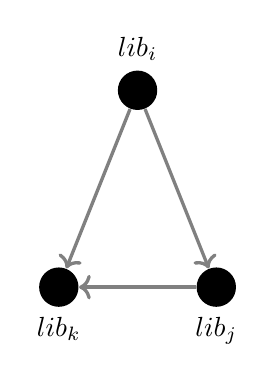
\begin{tikzpicture}[
         roundnode/.style={circle, fill=black, minimum size=5mm},
        squarenode/.style={fill=black, text=red, minimum size=5mm},
     ]
    \begin{scope}
         \node[roundnode, label=above:$lib_i$] (s2_proji) at (3, 2.5) {};
        \node[roundnode, label=below:$lib_j$] (s2_projj) at (4,0) {};
         \node[roundnode, label=below:$lib_k$] (s2_projk) at (2,0) {};
     \end{scope}

     \begin{scope} [every edge/.style={draw=gray, very thick}]
         \path [->] (s2_proji) edge (s2_projj);
         \path [->] (s2_proji) edge (s2_projk);
         \path [->] (s2_projj) edge (s2_projk);
     \end{scope}
     \end{tikzpicture}
    
     \caption{Example dependency graph for a given time period}
     \label{fig:lib}
     \vspace{2ex}
 \end{figure}
\begin{figure}[t]
    \centering

    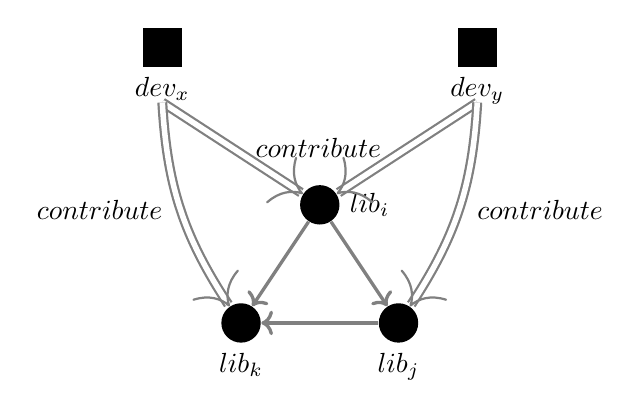
\begin{tikzpicture}[
        roundnode/.style={circle, fill=black, minimum size=5mm},
        squarenode/.style={fill=black, text=red, minimum size=5mm},
    ]
    \begin{scope}
        
        \node[roundnode, label=right:$lib_i$] (s2_proji) at (4, 1.5) {};
        \node[roundnode, label=below:$lib_j$] (s2_projj) at (5,0) {};
        \node[roundnode, label=below:$lib_k$] (s2_projk) at (3,0) {};
        
        \node[squarenode, label=below:$dev_x$] (s3_devx) at (2, 3.5) {};
        
        \node[squarenode, label=below:$dev_y$] (s3_devy) at (6, 3.5) {};
        
    \end{scope}

    \begin{scope} [every edge/.style={draw=gray, very thick}]
        \path [->] (s2_proji)  edge  (s2_projj);
        \path [->] (s2_proji) edge (s2_projk);
        \path [->] (s2_projj) edge (s2_projk);
        
    \end{scope}
    \begin{scope} [every edge/.style={draw=gray, thick, double distance=2pt}]
        \path [->] (6, 2.8) edge node[left = 2mm] {$contribute$} (s2_proji);
        \path [->] (6, 2.8) edge[bend left=15] node[right = 1mm] {$contribute$} (s2_projj);
        \path [->] (2, 2.8) edge node[right = 2mm] {$$} (s2_proji);
        \path [->] (2, 2.8) edge[bend right=15] node[left = 1mm] {$contribute$} (s2_projk);
    \end{scope}
    \end{tikzpicture}
\end{figure}
\begin{figure}[t]
    \centering
    \begin{tikzpicture}[
        roundnode/.style={circle, fill=black, minimum size=5mm},
        squarenode/.style={fill=black, text=red, minimum size=5mm},
    ]
    \end{tikzpicture}
\caption{Example Dependency-Contribution graph showing relationships between contributions and dependencies}
 \label{fig:dc-graph}
\end{figure}

This is just one example of the type of research that is enabled by access to heterogeneous data related to software package ecosystems.

\smallskip\noindent\textbf{Peril 1.}\textit{
 Developers might use different identifiers when contributing to different parts of a software package ecosystem, e.g., when contributing to different libraries.}\\
 
When modelling using such graphs, there is a threat that contributors may use multiple identifiers (i.e., $c_x$ and $c_y$ are the same contributor).
This is a well-known research problem, and there has been work to merge these accounts, such as \cite{wiese2016mailing}.
GitHub has introduced mechanisms such as two-factor authentication\footnote{\url{https://docs.github.com/en/authentication/securing-your-account-with-two-factor-authentication-2fa/configuring-two-factor-authentication}} to counteract the issue of multiple identifiers.
This is since developers might be less likely to switch accounts if it requires cumbersome authentication.


\smallskip\noindent\textbf{Peril 2.}\textit{
Developers' contributions to software package ecosystems might be interspersed with bot contributions, e.g., automated dependency updates.}\\

The rise of automation and artificial intelligence has led to much work on the integration of automated scheduling (i.e., bots) into software development workflows \cite{Storey2016, Farooq2016, Wessel2018, Erlenhov2019, bot_modify_wf} to name a few. These bots are designed to perform specific tasks within a software package ecosystem. For example, a bot may be programmed to automatically update dependencies, test code changes, or deploy software to production. As an example, the Google APIs repo-automation-bots project lists bots for automated labelling of issues and pull requests, automated approval of pull requests, and triggering releases.\footnote{\url{https://github.com/googleapis/repo-automation-bots}}
Bots perform common maintenance tasks in many software projects and are now commonplace \cite{Beschastnikh2017, Urli2018,BIMAN,bot_or_not}.
Especially with bots such as dependabot (automated pull requests to update configurations to reduce the risk of vulnerability threats),\footnote{\url{https://github.com/dependabot}} more and more automation has caused a lot of noise in the contributions between projects.
There are also bots for communication and documentation \cite{Urli2018, Lin2016, Lebeuf2017a}.

To be able to draw accurate conclusions about what humans are doing in software package ecosystems, researchers should consider distinguishing between bot and human contributions.
It is also important to differentiate this from other contributions \cite{maeprasart2022understanding}.
The research community has responded well, with a wide range of techniques and tools to mitigate this peril \cite{Bodegha2021, golzadeh2022accuracy}.

\smallskip\noindent\textbf{Peril 3.}\textit{
Not all developer activities in software package ecosystems are accessible to the public, e.g., library use in proprietary settings.
}\\

Not all developer activities in software package ecosystems are accessible to the public, e.g., when the boundary between open source and industry is blurred \cite{stol2014inner}, which presents a challenge for researchers who aim to study the development process. This is particularly true in proprietary settings where software development is performed behind closed doors or is open source for a limited time period, thus resulting in the artefacts not permanently being publicly available.
This can make it difficult to understand the broader ecosystem in which a software project is developed.
Proprietary settings may lead to non-standardisation in software development practises. Different software projects may use different management systems and tools, making it difficult to accurately compare and analyse software development activities across various projects. For example, some projects may use communication, documentation, and other management tools not captured on the same platform \cite{montgomery2022alternative}. For example, some projects might use Bugzilla instead of issues and pull requests for their bug and code review systems, while others may use Discord, Slack channels, or email threads for their communication needs.

This lack of standardisation in software development practises presents a challenge for researchers who study the software package ecosystem and understand the development process. To address this issue, researchers should strive to collect data from a diverse set of projects to gain a comprehensive understanding of the software package ecosystem. In addition, researchers may need to adjust their methodologies or data collection techniques to accommodate the different tools and practises used by different software projects.

\subsection{Defining Components and their Dependencies}

\smallskip\noindent\textbf{Promise 2.}\textit{
Researchers can access a software package ecosystem's dependency network through package managers and registries, e.g., npm lists the dependencies and dependents for over a million libraries.}\\


With the rise of curated datasets like libraries.io, researchers can now recover and model dependency relations between software units using pre-extracted datasets.
Table \ref{tab:PM_features} shows examples of popular package managers mined from the libraries.io dataset in 2020. 

\begin{table*}[]
\caption{Summary of 13 package managers from libraries.io as ranked by TIOBE in 2020}
 \label{tab:PM_features}
 \centering
\begin{tabular}{@{}llrlll@{}}
\toprule
\begin{tabular}[c]{@{}l@{}}Package \\ Ecosystem\end{tabular} & \begin{tabular}[c]{@{}l@{}}Programming \\ Language\end{tabular} &  \begin{tabular}[c]{@{}l@{}}Tiobe \\ Rank\end{tabular} & Environment & \begin{tabular}[c]{@{}l@{}}Dependency \\ Tree\end{tabular} & \begin{tabular}[c]{@{}l@{}}Package   \\Archive link\end{tabular}\\ \midrule
PyPI & Python & 2 & Python & Flat & pypi.org  \\
Maven & Java & 3 & JVM & Flat & Maven.org  \\
Bower & JavaScript & 7 & Node.js & Flat & bower.io  \\
Meteor & JavaScript & 7 & Node.js & Nested & atmospherejs.com \\
npm & JavaScript & 7 & Node.js & Nested (v2) & npmjs.com  \\
Packagist & PHP & 8 & PHP & Flat & packagist.org \\
Puppet & Ruby & 13 & Ruby MRI & Flat & forge.puppet.com  \\
RubyGems & Ruby & 13 & Ruby MRI & Flat & rubygems.org  \\
CRAN & R & 14 & RStudio & Flat & cran.r-project.org  \\
CPAN & Perl & 15 & Perl & Flat & metacpan.org  \\
GO & Golang & 20 & Go & Flat & pkg.go.dev  \\
NuGet & C\#, VB & 5, 6 & .NET & Flat & nuget.org \\
Anaconda & Python, R, C\# & 2, 14, 5 & Anaconda & Flat & anaconda.org  \\ \bottomrule
\end{tabular}
\end{table*}

\smallskip\noindent\textbf{Peril 4.}\textit{
Different software package ecosystems define the concept of ``dependency'' differently, e.g., by allowing or not allowing different versions of a library on the same dependency tree.
}\\

Different software package ecosystems have varying definitions of what constitutes a dependency. For example, some ecosystems may allow multiple versions of a library to exist on the same dependency tree, while others may restrict developers to a single version of a library \cite{Islam}. These restrictions are often based on the programming language being used, as different languages have different approaches to managing dependencies. It is important to consider the restrictions on dependency relationships when studying software package ecosystems, as they can have a major impact on the development process. For example, the ability to use multiple versions of a library on the same dependency tree can greatly simplify the process of updating dependencies and can make it easier to resolve conflicts between libraries.

One way to visualise the impact of these restrictions is to compare the difference between a nested dependency tree and a directed dependency tree, as shown in Figure \ref{fig:nest}.\footnote{Taken from \url{https://npm.github.io/how-npm-works-docs/npm3/how-npm3-works.html}} This distinction is important because it highlights the different ways that a software unit can depend on different versions of the same library.
In this example, npm v3 creates the dependency tree based on the installation order, therefore flattening unnecessary nested dependencies (i.e., B v1.0 in cyan). This reduces the complexity of a nested tree by resolving some of the transitive dependencies (nested dependencies).

\begin{figure}
	\centering
	\includegraphics[width=.8\textwidth]{book/chapter-promisesandperils/pics/nestedv2.jpg}
	\caption{Difference between flat and nested dependencies}
	\label{fig:nest}
\end{figure}

\smallskip\noindent\textbf{Peril 5.}\textit{
Developers might declare a dependency to other parts of a software package ecosystem but not use it, e.g., because they failed to update its removal.
}\\

It is common for developers to declare dependencies on other parts of the software package ecosystem but not always use them. This can happen for various reasons, such as forgetting to remove the dependency after it is no longer needed. This can pose a challenge for researchers who are trying to extract dependencies from package managers, like those in configuration files, as there may be inconsistencies between the listed dependencies and what is actually being compiled and used by the code. This can lead to a biased understanding of the software package ecosystem and the relationships between software components.

To address this issue, there have been numerous efforts to track the actual library dependencies compiled and executed in software systems. These efforts aim to provide a more accurate understanding of the dependencies and the relationships between software components. For example, research has been conducted on the use of dynamic analysis to track compiled dependencies in real time and on the development of tools to automatically detect and track executed dependencies \cite{Zapata:ICSME2018, Ponta2018,Chinthanet:ASE2020}.

\subsection{Defining Boundaries and Completeness}

\smallskip\noindent\textbf{Promise 3.}\textit{
Researchers can use the boundaries of software package ecosystems to study communities of developers, e.g., developers contributing to and/or benefiting from the npm ecosystem.
}\\

Following Promise 2, the emergence of package managers has also led to studies that approximate software communities.
Using the libraries.io dataset, researchers were able to study projects that host libraries that use package managers.
Researchers have used this dataset to compare different library ecosystems \cite{kikas.2017,decan:emse:2019,CogoDown2019}.


\smallskip\noindent\textbf{Peril 6.}\textit{
Package managers do not always represent software package ecosystems, their communities, or their sub-communities, e.g., in cases where multiple package managers exist.
}\\

Package managers are a fundamental aspect of software package ecosystems, but do not always fully represent the complex relationships and interactions that occur within a community of developers and users, as shown in Table~\ref{tab:PM_features}. In some cases, multiple package managers exist for the same programming language, creating a complex landscape of software libraries and dependencies that are not always easily understood. For instance, Bower and Meteor manage npm libraries, which can lead to confusion and overlap in the management of dependencies.

Similarly, Java, Scala, Android, and other Java-based open source communities all use the Maven package manager, but each of these communities has its own unique set of libraries, dependencies, and development practises. Researchers should be aware of the limitations of package managers when studying software package ecosystems, and consider the broader context and relationships that exist within these communities. 

\smallskip\noindent\textbf{Peril 7.}\textit{
Lack of activity in parts of a software package ecosystem does not necessarily indicate project failure, e.g., when highly depended-upon libraries are feature-complete.
}\\

It is important to note that lack of activity in a part of a software package ecosystem does not always mean project failure \cite{coelho2017modern}. In some cases, highly relied-upon libraries that have reached feature-completeness may see little activity, but continue to be used by the software community. 

However, it is still important to consider the long-term sustainability of these libraries, especially given the rate at which technology and software development practises change. This has become a topic of interest in recent years, and researchers have explored best practises for sustaining open source projects and ensuring their continued success \cite{Ait2022,valiev2018ecosystem}. Understanding the factors that contribute to project sustainability is important to ensure the longevity and continued growth of software package ecosystems.

\smallskip\noindent\textbf{Peril 8.}\textit{
Sampling from a software package ecosystem is challenging since sub-setting might alter the dependency network, e.g., by breaking dependency chains.
}\\

Sampling from a package ecosystem is not straightforward, as the sample composition can be significantly affected due to missing dependency links between libraries. For instance, a subset of the ecosystem might alter the dependencies between libraries, leading to the breakdown of the dependency chains. This could lead to an incomplete picture of the software package ecosystem, leading to incorrect conclusions from a study. To minimise this risk, researchers should carefully consider the boundaries of their study and choose the appropriate sampling method based on the research questions and goals. For example, researchers could focus on popular, highly dependent, or risk-vulnerable aspects of the ecosystem as a starting point. 
For some ecosystems, the number of downloads, GitHub stars, and watchers are other aspects for the researcher to utilise.


\smallskip\noindent\textbf{Peril 9.}\textit{
Sampling from a software package ecosystem is challenging since the dependency network changes over time, e.g., when dependencies are added, removed, upgraded, or downgraded.
}\\

The dynamic nature of package ecosystems and the constant changes to their dependencies can impact the generalisability of the results. Therefore, it is important to also consider the time granularity of the analysis. For example, if the goal is to understand the evolution of dependencies over time, a finer time granularity may be necessary to capture the smaller changes and trends. However, if the goal is to understand the overall structure and relationships within the ecosystem, a coarser time granularity may be sufficient. Based on recent studies \cite{wattanakriengkrai2022giving,valiev2018ecosystem,Mirsaeedi:icse2020, Brindescu:emse2020, Nassif:icsme2017}, a three-month window seems appropriate for some studies.
Another level of granularity to consider is the size of the component. For instance, there are cases where a single package may contain more than one repository, especially for large library frameworks. 
The granularity also depends on the nature of the ecosystem itself. For instance, researchers should understand whether the ecosystem comprises library packages (e.g., PyPI), plugins (e.g., Eclipse), or is a library distribution (e.g., Android).



\subsection{Analysing and Visualising the Data}

\textbf{Peril 10.}\textit{
Analysing and visualising entire software package ecosystems is challenging due to their size, e.g., in terms of nodes and edges in the network.
}\\

The size of software package ecosystems implies large data sets, which can be overwhelming for tools and algorithms to analyse and display. Therefore, it may be necessary to make choices about the granularity of the data included in the analysis and visualisation. Another alternative is to focus on the most critical parts of the software package ecosystem, such as the high-level structure, highly dependent packages, or parts of the system that pose a risk to security and reliability. 
The key is to strike a balance between detail and simplicity, providing a meaningful representation of the ecosystem while being able to handle the complexity of its size.


\section{Application: When to Apply Which Peril}
\label{PPM:sec:application}

We include a disclaimer stating that not all perils are applicable to every mining situation. To demonstrate the practical application of our perils and their mitigation, we present two case studies that involve mining the software package ecosystem. Each case study has a distinct research objective and focusses on a specific dataset to be mined.

\subsection{Two Case Studies}
Table \ref{tab:cases} presents the two case studies we have selected for this analysis.
The \textit{first case} involves mining for contributions congruent to dependency updates \cite{wattanakriengkrai2022giving}. 
In this work, the authors mine GitHub repositories for Pull Requests and Issues that were submitted and merged congruent to dependency updates within the npm ecosystem. 
The \textit{second case} involves mining communication data for the Eclipse ecosystem \cite{Nugroho2021}. Although the second case does not mine for dependency relations (i.e., use relations),  we show that these perils still apply when mining for other relationships in an ecosystem.
Moreover, the second case studies the Eclipse ecosystem, which is a different dataset compared to the more popular GitHub dataset.

\subsection{Applying Perils and their Mitigation Strategies}
Table \ref{tab:perilsapp} provides a summary of the perils that can be applied to each of the case studies. We will now go into the details of mitigation strategies based on these perils. 
For better organisation and understanding, we have grouped the perils according to the four logical processes for mining.

\smallskip\noindent\textbf{Information to Mine}. 
The first set of mitigation strategies, which addresses perils 1-3, focusses on planning which information to mine. There are two primary strategies that researchers can employ:


\begin{enumerate}
    \item Researchers should use research tools and techniques to remove noise and other biases in the dataset, such as bot detection and the handling of multiple identities. This strategy was implemented in both case studies, as contributions and discussions often have the potential to involve bots or developers with multiple identities.
\item Depending on the research goals, researchers should recognise that not all contributions are equal and filter the dataset accordingly.
\end{enumerate}

We applied these two strategies to both cases. In the first case, the goal was to capture all congruent contributions, so we filtered out contributions made to libraries without dependencies. Since all npm packages are listed in the registry, Peril 3 (private activities) did not apply.
In the second case, we addressed Peril 1 by conducting a qualitative analysis to ensure that the member identities were not duplicated, as Eclipse developers were known to change identities. To mitigate Peril 2, we removed bot responses. For the second case, since all forum data is made public, Peril 3 did not apply.


\begin{table}
\centering
\caption{Description of the research objectives and datasets for the case studies}
 \label{tab:cases}
\begin{tabular}{lp{5cm}r} 
\toprule
\textbf{Case Study} & \textbf{Research Objective}                                                          & \textbf{Datasets}           \\
\midrule
Wattanakriengkrai \etal \cite{wattanakriengkrai2022giving}             & Explore code contributions between library and client (i.e, use-relations)  & libraries.io\\
& &  GitHub API \\
Nugroho \etal \cite{Nugroho2021}                & Explore discussion contributions between contributors (i.e., contributions) & Eclipse API                \\
\bottomrule
\end{tabular}
\end{table}

\begin{table}
\centering
\caption{Application of each peril to the case studies}
 \label{tab:perilsapp}
\begin{tabular}{rp{8cm}ccc} 
\toprule                   
& \textbf{Perils}       & case 1      & case 2                 \\
                                                                               & & npm  & Eclipse   \\
\midrule
\textbf{P1} &Developers might use different identifiers when contributing to different parts of a software package ecosystem, e.g., when contributing to different libraries.                             &    \CheckedBox         &          \CheckedBox           \\ 
%\hline
\textbf{P2} & Developers' contributions to software package ecosystems might be interspersed with bot contributions, e.g., automated dependency updates.                                                      &      \CheckedBox               &      \CheckedBox               \\ 
%\hline
\textbf{P3} & Not all developer activities in software package ecosystems are accessible to the public, e.g., library use in proprietary settings.                                                         &         -           &      \CheckedBox               \\ 
%\hline
\textbf{P4} & Different software package ecosystems define the concept of \`{}\`{}dependency'' differently, e.g., by allowing or not allowing different versions of a library on the same dependency tree. &         \CheckedBox       &     -                            \\ 
%\hline
\textbf{P5} & Developers might declare a dependency to other parts of a software package ecosystem but not use it, e.g., because they failed to update its removal.                                        &     -           &  -    \\
%\hline
\textbf{P6} &Package managers do not always represent software package ecosystems, their communities, or their sub-communities, e.g., in cases where multiple package managers exist.                     &     -                   &  -                  \\
%\hline
\textbf{P7} & Lack of activity in parts of a software package ecosystem does not necessarily indicate project failure, e.g., when highly depended-upon libraries are feature-complete.                     &       \CheckedBox         &  -                           \\
%\hline
\textbf{P8} &Sampling from a software package ecosystem is challenging since sub-setting might alter the dependency network, e.g., by breaking dependency chains.                                         &        \CheckedBox        &     \CheckedBox                                \\
%\hline
\textbf{P9} &Sampling from a software package ecosystem is challenging since the dependency network changes over time, e.g., when dependencies are added, removed, upgraded, or downgraded.               &       \CheckedBox         &     -                          \\
%\hline
\textbf{P10} &Analysing and visualising entire software package ecosystems is challenging due to their size, e.g., in terms of nodes and edges in the network.                                  &        \CheckedBox      &      \CheckedBox               \\
\bottomrule
\end{tabular}
\end{table}

\smallskip\noindent\textbf{Defining Dependencies}. 
The second set of perils (Perils 4-5) is related to dependency relationships between software units, and only the first case study is applicable. To address these perils, researchers should adopt the following strategy:

\begin{enumerate}
    \item Researchers should not rely solely on listed dependencies in configuration files (e.g., pom.xml, package.json, etc.) as a measure of dependency between two components. Instead, code-centric approaches should be used to validate which libraries are actually depended upon.
\end{enumerate}

For example, in the first case, in addition to mining the configuration information, the authors also analysed the similarity of the source code contributions to address Peril 4. Regarding Peril 5, since the study's objective was to investigate changes to the configuration files, the risk of the update not being executed was deemed less important.
It is important to note that the second case study did not include dependency analysis and, therefore, these perils did not apply.

\begin{figure*}[]
    \centering
    \begin{subfigure}{0.9\linewidth}
         \includegraphics[width=1.1\textwidth]{book/chapter-promisesandperils/pics/congruentViz.jpg}
         \caption{Visualization of a Time analysis for 107,242 libraries.}
     \end{subfigure}
     \begin{subfigure}{0.9\linewidth}
         \includegraphics[width=1\textwidth]{book/chapter-promisesandperils/pics/eclipseViz.jpg}
         \caption{A Visual Topology map for 832,058 threads}
     \end{subfigure}
    \caption{Visualisation examples for the two case studies}
    \label{fig:visCase}
\end{figure*}

\smallskip\noindent\textbf{Defining Boundaries}.
The third set of perils (Perils 6-9) is related to the definition of boundaries and completeness and is relevant for both case studies. To mitigate these perils, we recommend the following strategies:

\begin{enumerate}
    \item Researchers should recognise that a dormant project does not necessarily mean that it is inactive. Instead, studies can use alternative heuristics, such as the number of dependents and dependencies, as better indicators of a project's importance in the ecosystem.
    \item Researchers should not rely solely on the programming language to define sub-communities. Using a common package manager for the programming language is a more effective rule of thumb for distinguishing boundaries.
    \item Researchers should avoid random sampling. Instead, sampling should be tailored to the research goals by considering factors such as an appropriate time window or focussing on specific attributes of components (e.g., most dependents, most popular, most contributors).
\end{enumerate}


Peril 6 did not apply to any of the case studies. 
Particularly for the first case, since the goal was to explore the npm package ecosystem, we assumed that the boundaries were clearly defined by the npm registry. 
Similarly, the second case study used the generic Eclipse platform as the boundary. 
Peril 7 was applied to the npm study, while Peril 8 was applied to both case studies. 
As a result, the two cases conducted a qualitative analysis of the dataset to gain deeper insights.
In the first case study, a three-month time window was created to capture dependencies. 
For the second case study, forum contributors were sampled into three groups (i.e., junior, member, or senior) according to the sliding window of their contributions. 

\smallskip\noindent\textbf{Visualisation}.
The final peril (Peril 10) relates to visualisation, which can be challenging due to the vast size and complexity of software ecosystems. As it is not feasible to visualise every aspect of an ecosystem simultaneously, a focused approach is necessary. A mitigation strategy is to select specific attributes of the ecosystem (e.g., the most dependent, most popular, and most contributions) that align with the research needs and objectives. 

Figure \ref{fig:visCase} shows two cases where visualizations are employed to gain insights, especially for large datasets.
In the first figure (a), we visualize the distributions of the data set and applied the appropriate statistical tests, along with the effect size, to test our hypotheses and answer research questions. 
In the second example (b), although not directly related to package ecosystems, the authors utilized a topological visualization \cite{Lum2013ExtractingIF} to gain insights on the over 800,000 forum threads of discussions. 



\section{Chapter Summary}
In this chapter, we explore the various aspects of mining information from the software package ecosystem, presenting three promises and ten perils that researchers should be aware of when undertaking such tasks. The chapter is structured around four key processes for mining: 1) Planning what Information to Mine, 2) Defining Components and their Dependencies, 3) Defining Boundaries and Completeness, and 4) Analysing and Visualising the Data. To help new and experienced researchers navigate these challenges, we introduced the SUG model, which can serve as a valuable tool to minimise threats to validity. Although some perils may be more relevant to specific research objectives, our aim is to equip researchers with the knowledge and resources needed to confidently gather and integrate software package ecosystem data into their work.
%Software library recommendation and usage analysis
% %Semantic labeling three-letter-code: SLU (e.g. \chapter{SLU})

% 
\title{Promises and Perils of Mining \\ Software Package Ecosystem Data}
\author{Raula Gaikovina Kula \and Katsuro Inoue \and Christoph Treude}
\institute{Raula Gaikovina Kula \at Nara Institute of Science and Technology, Japan, \email{raula-k@naist.jp}
\and Katsuro Inoue \at Nanzan University, Japan \email{ inoue599@nanzan-u.ac.jp}
\and  Christoph Treude \at The University of Melbourne, Australia \email{christoph.treude@unimelb.edu.au}}

\maketitle
\label{PPM:ch}
\abstract*{The use of third-party packages is becoming increasingly popular and has led to the emergence of large software package ecosystems with a maze of inter-dependencies. Since the reliance on these ecosystems enables developers to reduce development effort and increase productivity, it has attracted the interest of researchers: understanding the infrastructure and dynamics of package ecosystems has given rise to approaches for better code reuse, automated updates, and the avoidance of vulnerabilities, to name a few examples. But the reality of these ecosystems also poses challenges to software engineering researchers, such as: How do we obtain the complete network of dependencies along with the corresponding versioning information? What are the boundaries of these package ecosystem? How do we consistently detect dependencies that are declared but not used? How do we consistently identify developers within a package ecosystem? How much of the ecosystem do we need to understand to analyse a single component? How well do our approaches generalise across different programming languages and package ecosystems? In this chapter, we review promises and perils of mining the rich data related to software package ecosystems available to software engineering researchers.}

\abstract{The use of third-party packages is becoming increasingly popular and has led to the emergence of large software package ecosystems with a maze of inter-dependencies. Since the reliance on these ecosystems enables developers to reduce development effort and increase productivity, it has attracted the interest of researchers: understanding the infrastructure and dynamics of package ecosystems has given rise to approaches for better code reuse, automated updates, and the avoidance of vulnerabilities, to name a few examples. But the reality of these ecosystems also poses challenges to software engineering researchers, such as: How do we obtain the complete network of dependencies along with the corresponding versioning information? What are the boundaries of these package ecosystems? How do we consistently detect dependencies that are declared but not used? How do we consistently identify developers within a package ecosystem? How much of the ecosystem do we need to understand to analyse a single component? How well do our approaches generalise across different programming languages and package ecosystems? In this chapter, we review promises and perils of mining the rich data related to software package ecosystems available to software engineering researchers.}

%%%%%%%%%%%%%%%%%%%%%%%%%%%%%%%%%%%%%%%%%%%%%%%%%%%%%%%%%%%%%%%%%%

\section{Introduction}
\label{PPM:sec:definition}

Third-party libraries are a great way for developers to incorporate code without having to write their own for every functionality required. By using these libraries, developers can save time and energy while still getting the functions they need.
Using third-party libraries is becoming increasingly popular and has led to the emergence of large software package ecosystems such as npm. While these ecosystems offer many benefits, they also come with risks, such as software vulnerability attacks \cite{Chinthanet:ASE2020}.

Large software package ecosystems are a treasure trove for researchers who can investigate a wide range of questions. For example, by studying activity in large ecosystems, researchers can identify which libraries are the most popular and learn what characteristics make them successful \cite{kikas.2017,decan:emse:2019}.
Additionally, research on large ecosystems can help developers understand how to protect their code from malicious actors who may attempt to exploit vulnerabilities or insert malware into popular libraries.
Studying large software package ecosystems can help us better understand the dynamics of open source development in general. Open source development is a complex process that involves many different stakeholders working together (or sometimes competing) to create valuable code that anyone can use or improve upon. By understanding how these interactions play out in different types of ecosystem structures -- including those with many small projects versus few very large ones -- we can develop insights that might be applicable more broadly across other types of collaborative systems.

In this chapter, we identify and discuss promises and perils during the mining process, ranging from planning what information to mine from the ecosystem to analysing and visualising the mined data. 
Therefore, the chapter is broken down into these logical processes of mining ecosystem data: 1) Planning what Information to Mine, 2) Defining Components and their Dependencies, 3) Defining Boundaries and Completeness, and 4) Analysing and Visualising the Data.

This chapter is intended for researchers and practitioners who are interested in exploring and exploiting software package ecosystem information from a diverse range of sources that are publicly available. 
We also highlight the pitfalls to consider during the mining process, particularly when these pitfalls could lead to a misinterpretation of the analysis and results. 
The chapter is written in a manner that encourages newcomers who have little or no experience or who are interested in utilising ecosystem data across different disciplines outside of software engineering.
Our goal is to get new researchers quickly accustomed to gathering ecosystem information for their research.


\section{A Component-based Software Ecosystem}

Defined as a component-based software ecosystem, we suggest using the term `software package ecosystem' as a suitable term for the symbiotic relationships among third-party library components (as software projects or repositories), as these libraries and their dependent clients coexist on the same technological platform, therefore sharing the same environment and other internal and external factors (e.g., security threats, sharing contributions, etc.).
Please refer to the Introduction chapter for an in-depth definition of the different types of software ecosystems.
We present our interpretation of the software package ecosystem in Kula et al.~\cite{KulaSANER18}, where we formally define a package ecosystem using a Software Universe Graph (SUG).
This is modelled as a structured abstraction of the evolution of software systems and their library dependencies over time.

%%%%%%%%%%%%%%%%%%%%%%%%%%%%%%%%%%%%%%%%%%
\begin{figure*}
	\centering
	\includegraphics[width=.7\textwidth]{book/chapter-promisesandperils/pics/UniversalExample.jpg}
	\caption{Conceptual example of the Software Universe Graph, depicting the use and update relationships between different software units.}
	\label{fig:SUG}
\end{figure*}
%%%%%%%%%%%%%%%%%%%%%%%%%%%%%%%%%%%%%%%%%%%%%


\paragraph{\textbf{Component-based Representation as a Software Universe Graph}}
\label{PPM:sec:SUG}

First introduced by Kula et al.~\cite{KulaSANER18}, the \textit{Software Universe Graph} (SUG) is a structural abstraction of the software ecosystem of third-party libraries.
Figure \ref{fig:SUG} provides an illustration of the different relationships within the graph.
Let $G= (N,E)$ represent a graph $G$. $N$ is a set of nodes, each node representing a software unit. 
We define a software unit as a version instance of any software program. 

The authors then present the \textit{use} and \textit{update} relationships that exist in the ecosystem.
Hence, the edges $E$ are composed of $E_{use}$ and $E_{update}$. $E_{use}$ is a set of \textit{use-relations} and $E_{update}$ is a set of \textit{update-relations}.

\begin{definition}
An edge $u \rightarrow v \in E_{use}$ means that $u$ uses $v$. The defined functions of $E_{use}$ are:

\begin{equation}
\small
\small \use(u)\equiv \{v|u \rightarrow v\}
\normalsize
\end{equation}
\begin{equation}
\small
\small \useBy(u)\equiv \{v|v \rightarrow u\}
\normalsize
\end{equation}
\end{definition}

Use-relations can be extracted from either the source code or configuration files. 
As shown in Figure \ref{fig:SUG}, node $a1$ uses node $x1$. 
In addition, node $x1$ is used by nodes $a1$, $q1$, and $q2$. Parallel edges for node pairs are not allowed.

\begin{definition}
We represent an update relation from node $a$ to $b$ using $ a \Rightarrow b $, which means that the newer update $b$ was released from node $a$ and is defined as:
\begin{equation}
\small a \Rightarrow b \in E_{update}
\end{equation}
\end{definition}

Update relations refer to when a successive release of a software unit is made available. Figure \ref{fig:SUG} shows that node $q1$ is first updated to node $q2$. Later, node $q2$ is updated to the latest node $q3$. Hence, $q1 \Rightarrow q2 \Rightarrow q3$.
Note that an update should not be confused with forking. 
We distinguish a fork as a separate software unit. 
Each node in the SUG should be denoted by three attributes: \texttt{<name,release,time>}.  
For a node $u$, we define:

\begin{itemize}
	\item \textbf{u.name} Name is the string representation identifier of a software unit.
	We introduce the name axiom: For nodes $u$ and $v$, if $u \Rightarrow v$, then $u.name = v.name$ holds.
	
	\item \textbf{u.release}. Release refers to the specific assigned change reference for a software unit. For nodes $u$ and $v$, if $u \Rightarrow v$
	then $v$ is the immediate successor of $u$. Note that the versioning pattern may vary from project to project. 
	\item \textbf{u.time}. Time refers to the time stamp at which node $u$ was released. For nodes $u$ and $v$ of $u \Rightarrow v$, $u.time < v.time$.
\end{itemize}

\begin{figure}
	\centering
	\includegraphics[width=.8\textwidth]{book/chapter-promisesandperils/pics/TemporalSUG.jpg}
	\caption{Temporal property of the SUG}
	\label{fig:SUGTemp}
\end{figure}

\begin{definition}
    
	The SUG has temporal properties.
This describes the simultaneity or ordering in reference to time. Let SUG $G = (N, E) $ be at time $t$. At time $t^{\prime} > t$, we observe an extension of $G$, such that:

\begin{equation}
\small G^{\prime} = (N \cup \Delta N, E \cup \Delta E)
\end{equation}
where $\Delta E \cap (N \times N) = \emptyset$
\end{definition}

Figure \ref{fig:SUGTemp} illustrates the temporal properties of the SUG. 
Here, it is observed that $G'$ is composed of $G$ augmented with newly added node $a3$ and its corresponding $a3 \rightarrow x2$ and $a2 \Rightarrow a3$ relations.
A SUG grows monotonically over time with only additions.
Here, we consider that modification or deletion changes on the SUG do not occur. 

\begin{definition}
    A timed SUG specifies the state of the SUG at any point in time.
So for an SUG $G=(N,E)$, we represent a timed SUG $G_{t}$ at time $t$ as a sub-graph of $G$. Formally,
\begin{equation}
\small G_t\equiv(N_{t}, E_{t})
\end{equation}
where $N_{t} = \{u|u \in N, u.time \leq t \}$ and $E_t = \{ e | e \in E \wedge e \in  N_t \}$
\end{definition}
	


\section{Data Sources}
Researchers can use various datasets to model the ecosystem using the SUG model of usage and update relationships.
The most obvious data source that has revolutionised data mining in the software engineering domain is the GitHub platform. 
Established in 2008, and then purchased by Microsoft in 2020, GitHub is home to various popular Open Source Software. 
GitHub is built on the git version control system and is useful for storing all changes made to a repository. 
In the case of the SUG, a GitHub repository can represent one software unit, whose depend relations can be extracted via a configuration file (such as the package.json file for JavaScript projects).
The repository should also contain the release information that holds the update relations.
Due to its large size, researchers and the GitHub team have made available datasets for researchers to mine, for example through the GitHub API/Graph QL.\footnote{\url{https://docs.github.com/en/graphql}} This is the backend Application Programming Interface (API) that can be used to query large amounts of data on GitHub. Most researchers use the API to download and mine information from the GitHub platform. 
It is important to note that while GitHub introduced a new feature of Dependency Graphs to map the depend relationship,\footnote{\url{https://docs.github.com/en/code-security/supply-chain-security/understanding-your-software-supply-chain/about-the-dependency-graph}} most older projects do not have this feature.
In this case, the researcher would need to manually extract and query the configuration files for dependency information. 

We refer to the first chapter for additional information on data sources for mining software ecosystems. 

\section{Promises and Perils}
\label{PPM:sec:promisesperils}

Using the SUG model of depend and use relations and the available datasets, we can now present our promises and perils of mining ecosystem information.

\subsection{Planning What Information to Mine}

\textbf{Promise 1.}\textit{
Researchers can access and link heterogeneous data related to software package ecosystems, e.g., package registries and bug trackers.}\\

When planning what information to mine from the ecosystem, researchers do not need to limit themselves to the usage and update relationship information.
Platforms that host software repositories include other software management systems such as bug trackers.
For example, GitHub allows researchers to manage GitHub Pull Requests, Issues, and Discussions not only for one project, but for multiple projects.
GitHub provides three management systems that are related to a software repository:

\begin{itemize}
    \item \textit{GitHub Discussions}\footnote{\url{https://docs.github.com/en/discussions}} - The GitHub Discussions forum is a collaborative communication forum for the community around an open source or internal project. Community members can ask and answer questions, share updates, have open-ended conversations, and follow along on decisions affecting the community's way of working.
    \item \textit{GitHub Pull Requests}\footnote{\url{https://docs.github.com/en/pull-requests}} - Pull Requests allow other developers from an ecosystem to make a contribution to a software repository. Pull requests also allow maintainers to discuss and review potential changes with collaborators and add follow-up commits before changes are merged into the software.
    \item \textit{GitHub Issues}\footnote{\url{https://docs.github.com/en/issues}} - Issues are used to track ideas, feedback, tasks, or bugs for work on GitHub.
\end{itemize}

These three systems are examples of how developers contribute to both their own and other projects. 
Hence, to incorporate this information, we can extend the SUG model, creating a model that includes a contribution relationship \cite{wattanakriengkrai2022giving}.

% Note that other platforms may also have management systems, like GitLab, BitBucket and Eclipse.

\begin{definition}
	A Dependency-Contribution graph incorporates contributions by developers whose libraries are involved in dependency relationships. 
\end{definition}

In this work \cite{wattanakriengkrai2022giving}, the authors explore the congruence between dependency updates and developer contributions, based on the original concept of social-technical congruence \cite{stcCataldo2008} where developers contribution patterns are congruent with their coordination needs. Hence, the goal is to identify contributions that are congruent to dependency updates.
As shown in Figure \ref{fig:lib} the authors extend from the typical SUG graph model where $lib_i$ depends (use) on  $lib_k$ and  $lib_j$, while  $lib_j$ also depends on $lib_k$, to the example shown in Figure \ref{fig:dc-graph}.
Different to the SUG, the graph captures developers and their contributions (i.e., the square as $dev_x$ and $dev_y$ represent two different developers making a contribution).
Here contributions are defined as $c$ (Pull Request or Issue) that were submitted to both a library and the client that depends on that library.
Hence, the graph can show contributions that are congruent to dependency changes for a software unit. 

\begin{figure}[t]
     \centering
     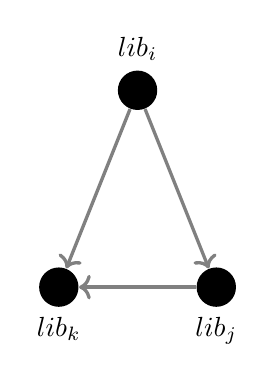
\begin{tikzpicture}[
         roundnode/.style={circle, fill=black, minimum size=5mm},
        squarenode/.style={fill=black, text=red, minimum size=5mm},
     ]
    \begin{scope}
         \node[roundnode, label=above:$lib_i$] (s2_proji) at (3, 2.5) {};
        \node[roundnode, label=below:$lib_j$] (s2_projj) at (4,0) {};
         \node[roundnode, label=below:$lib_k$] (s2_projk) at (2,0) {};
     \end{scope}

     \begin{scope} [every edge/.style={draw=gray, very thick}]
         \path [->] (s2_proji) edge (s2_projj);
         \path [->] (s2_proji) edge (s2_projk);
         \path [->] (s2_projj) edge (s2_projk);
     \end{scope}
     \end{tikzpicture}
    
     \caption{Example dependency graph for a given time period}
     \label{fig:lib}
     \vspace{2ex}
 \end{figure}
\begin{figure}[t]
    \centering

    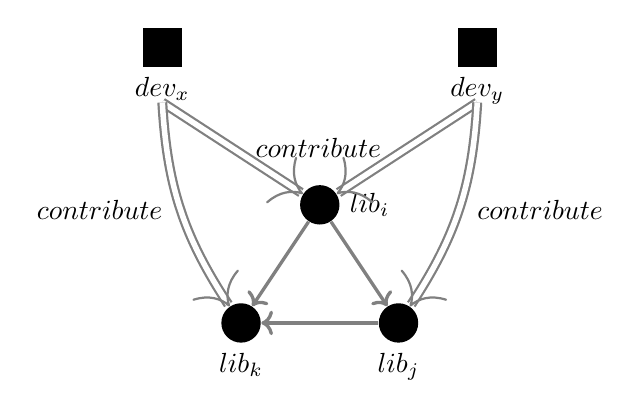
\begin{tikzpicture}[
        roundnode/.style={circle, fill=black, minimum size=5mm},
        squarenode/.style={fill=black, text=red, minimum size=5mm},
    ]
    \begin{scope}
        
        \node[roundnode, label=right:$lib_i$] (s2_proji) at (4, 1.5) {};
        \node[roundnode, label=below:$lib_j$] (s2_projj) at (5,0) {};
        \node[roundnode, label=below:$lib_k$] (s2_projk) at (3,0) {};
        
        \node[squarenode, label=below:$dev_x$] (s3_devx) at (2, 3.5) {};
        
        \node[squarenode, label=below:$dev_y$] (s3_devy) at (6, 3.5) {};
        
    \end{scope}

    \begin{scope} [every edge/.style={draw=gray, very thick}]
        \path [->] (s2_proji)  edge  (s2_projj);
        \path [->] (s2_proji) edge (s2_projk);
        \path [->] (s2_projj) edge (s2_projk);
        
    \end{scope}
    \begin{scope} [every edge/.style={draw=gray, thick, double distance=2pt}]
        \path [->] (6, 2.8) edge node[left = 2mm] {$contribute$} (s2_proji);
        \path [->] (6, 2.8) edge[bend left=15] node[right = 1mm] {$contribute$} (s2_projj);
        \path [->] (2, 2.8) edge node[right = 2mm] {$$} (s2_proji);
        \path [->] (2, 2.8) edge[bend right=15] node[left = 1mm] {$contribute$} (s2_projk);
    \end{scope}
    \end{tikzpicture}
\end{figure}
\begin{figure}[t]
    \centering
    \begin{tikzpicture}[
        roundnode/.style={circle, fill=black, minimum size=5mm},
        squarenode/.style={fill=black, text=red, minimum size=5mm},
    ]
    \end{tikzpicture}
\caption{Example Dependency-Contribution graph showing relationships between contributions and dependencies}
 \label{fig:dc-graph}
\end{figure}

This is just one example of the type of research that is enabled by access to heterogeneous data related to software package ecosystems.

\smallskip\noindent\textbf{Peril 1.}\textit{
 Developers might use different identifiers when contributing to different parts of a software package ecosystem, e.g., when contributing to different libraries.}\\
 
When modelling using such graphs, there is a threat that contributors may use multiple identifiers (i.e., $c_x$ and $c_y$ are the same contributor).
This is a well-known research problem, and there has been work to merge these accounts, such as \cite{wiese2016mailing}.
GitHub has introduced mechanisms such as two-factor authentication\footnote{\url{https://docs.github.com/en/authentication/securing-your-account-with-two-factor-authentication-2fa/configuring-two-factor-authentication}} to counteract the issue of multiple identifiers.
This is since developers might be less likely to switch accounts if it requires cumbersome authentication.


\smallskip\noindent\textbf{Peril 2.}\textit{
Developers' contributions to software package ecosystems might be interspersed with bot contributions, e.g., automated dependency updates.}\\

The rise of automation and artificial intelligence has led to much work on the integration of automated scheduling (i.e., bots) into software development workflows \cite{Storey2016, Farooq2016, Wessel2018, Erlenhov2019, bot_modify_wf} to name a few. These bots are designed to perform specific tasks within a software package ecosystem. For example, a bot may be programmed to automatically update dependencies, test code changes, or deploy software to production. As an example, the Google APIs repo-automation-bots project lists bots for automated labelling of issues and pull requests, automated approval of pull requests, and triggering releases.\footnote{\url{https://github.com/googleapis/repo-automation-bots}}
Bots perform common maintenance tasks in many software projects and are now commonplace \cite{Beschastnikh2017, Urli2018,BIMAN,bot_or_not}.
Especially with bots such as dependabot (automated pull requests to update configurations to reduce the risk of vulnerability threats),\footnote{\url{https://github.com/dependabot}} more and more automation has caused a lot of noise in the contributions between projects.
There are also bots for communication and documentation \cite{Urli2018, Lin2016, Lebeuf2017a}.

To be able to draw accurate conclusions about what humans are doing in software package ecosystems, researchers should consider distinguishing between bot and human contributions.
It is also important to differentiate this from other contributions \cite{maeprasart2022understanding}.
The research community has responded well, with a wide range of techniques and tools to mitigate this peril \cite{Bodegha2021, golzadeh2022accuracy}.

\smallskip\noindent\textbf{Peril 3.}\textit{
Not all developer activities in software package ecosystems are accessible to the public, e.g., library use in proprietary settings.
}\\

Not all developer activities in software package ecosystems are accessible to the public, e.g., when the boundary between open source and industry is blurred \cite{stol2014inner}, which presents a challenge for researchers who aim to study the development process. This is particularly true in proprietary settings where software development is performed behind closed doors or is open source for a limited time period, thus resulting in the artefacts not permanently being publicly available.
This can make it difficult to understand the broader ecosystem in which a software project is developed.
Proprietary settings may lead to non-standardisation in software development practises. Different software projects may use different management systems and tools, making it difficult to accurately compare and analyse software development activities across various projects. For example, some projects may use communication, documentation, and other management tools not captured on the same platform \cite{montgomery2022alternative}. For example, some projects might use Bugzilla instead of issues and pull requests for their bug and code review systems, while others may use Discord, Slack channels, or email threads for their communication needs.

This lack of standardisation in software development practises presents a challenge for researchers who study the software package ecosystem and understand the development process. To address this issue, researchers should strive to collect data from a diverse set of projects to gain a comprehensive understanding of the software package ecosystem. In addition, researchers may need to adjust their methodologies or data collection techniques to accommodate the different tools and practises used by different software projects.

\subsection{Defining Components and their Dependencies}

\smallskip\noindent\textbf{Promise 2.}\textit{
Researchers can access a software package ecosystem's dependency network through package managers and registries, e.g., npm lists the dependencies and dependents for over a million libraries.}\\


With the rise of curated datasets like libraries.io, researchers can now recover and model dependency relations between software units using pre-extracted datasets.
Table \ref{tab:PM_features} shows examples of popular package managers mined from the libraries.io dataset in 2020. 

\begin{table*}[]
\caption{Summary of 13 package managers from libraries.io as ranked by TIOBE in 2020}
 \label{tab:PM_features}
 \centering
\begin{tabular}{@{}llrlll@{}}
\toprule
\begin{tabular}[c]{@{}l@{}}Package \\ Ecosystem\end{tabular} & \begin{tabular}[c]{@{}l@{}}Programming \\ Language\end{tabular} &  \begin{tabular}[c]{@{}l@{}}Tiobe \\ Rank\end{tabular} & Environment & \begin{tabular}[c]{@{}l@{}}Dependency \\ Tree\end{tabular} & \begin{tabular}[c]{@{}l@{}}Package   \\Archive link\end{tabular}\\ \midrule
PyPI & Python & 2 & Python & Flat & pypi.org  \\
Maven & Java & 3 & JVM & Flat & Maven.org  \\
Bower & JavaScript & 7 & Node.js & Flat & bower.io  \\
Meteor & JavaScript & 7 & Node.js & Nested & atmospherejs.com \\
npm & JavaScript & 7 & Node.js & Nested (v2) & npmjs.com  \\
Packagist & PHP & 8 & PHP & Flat & packagist.org \\
Puppet & Ruby & 13 & Ruby MRI & Flat & forge.puppet.com  \\
RubyGems & Ruby & 13 & Ruby MRI & Flat & rubygems.org  \\
CRAN & R & 14 & RStudio & Flat & cran.r-project.org  \\
CPAN & Perl & 15 & Perl & Flat & metacpan.org  \\
GO & Golang & 20 & Go & Flat & pkg.go.dev  \\
NuGet & C\#, VB & 5, 6 & .NET & Flat & nuget.org \\
Anaconda & Python, R, C\# & 2, 14, 5 & Anaconda & Flat & anaconda.org  \\ \bottomrule
\end{tabular}
\end{table*}

\smallskip\noindent\textbf{Peril 4.}\textit{
Different software package ecosystems define the concept of ``dependency'' differently, e.g., by allowing or not allowing different versions of a library on the same dependency tree.
}\\

Different software package ecosystems have varying definitions of what constitutes a dependency. For example, some ecosystems may allow multiple versions of a library to exist on the same dependency tree, while others may restrict developers to a single version of a library \cite{Islam}. These restrictions are often based on the programming language being used, as different languages have different approaches to managing dependencies. It is important to consider the restrictions on dependency relationships when studying software package ecosystems, as they can have a major impact on the development process. For example, the ability to use multiple versions of a library on the same dependency tree can greatly simplify the process of updating dependencies and can make it easier to resolve conflicts between libraries.

One way to visualise the impact of these restrictions is to compare the difference between a nested dependency tree and a directed dependency tree, as shown in Figure \ref{fig:nest}.\footnote{Taken from \url{https://npm.github.io/how-npm-works-docs/npm3/how-npm3-works.html}} This distinction is important because it highlights the different ways that a software unit can depend on different versions of the same library.
In this example, npm v3 creates the dependency tree based on the installation order, therefore flattening unnecessary nested dependencies (i.e., B v1.0 in cyan). This reduces the complexity of a nested tree by resolving some of the transitive dependencies (nested dependencies).

\begin{figure}
	\centering
	\includegraphics[width=.8\textwidth]{book/chapter-promisesandperils/pics/nestedv2.jpg}
	\caption{Difference between flat and nested dependencies}
	\label{fig:nest}
\end{figure}

\smallskip\noindent\textbf{Peril 5.}\textit{
Developers might declare a dependency to other parts of a software package ecosystem but not use it, e.g., because they failed to update its removal.
}\\

It is common for developers to declare dependencies on other parts of the software package ecosystem but not always use them. This can happen for various reasons, such as forgetting to remove the dependency after it is no longer needed. This can pose a challenge for researchers who are trying to extract dependencies from package managers, like those in configuration files, as there may be inconsistencies between the listed dependencies and what is actually being compiled and used by the code. This can lead to a biased understanding of the software package ecosystem and the relationships between software components.

To address this issue, there have been numerous efforts to track the actual library dependencies compiled and executed in software systems. These efforts aim to provide a more accurate understanding of the dependencies and the relationships between software components. For example, research has been conducted on the use of dynamic analysis to track compiled dependencies in real time and on the development of tools to automatically detect and track executed dependencies \cite{Zapata:ICSME2018, Ponta2018,Chinthanet:ASE2020}.

\subsection{Defining Boundaries and Completeness}

\smallskip\noindent\textbf{Promise 3.}\textit{
Researchers can use the boundaries of software package ecosystems to study communities of developers, e.g., developers contributing to and/or benefiting from the npm ecosystem.
}\\

Following Promise 2, the emergence of package managers has also led to studies that approximate software communities.
Using the libraries.io dataset, researchers were able to study projects that host libraries that use package managers.
Researchers have used this dataset to compare different library ecosystems \cite{kikas.2017,decan:emse:2019,CogoDown2019}.


\smallskip\noindent\textbf{Peril 6.}\textit{
Package managers do not always represent software package ecosystems, their communities, or their sub-communities, e.g., in cases where multiple package managers exist.
}\\

Package managers are a fundamental aspect of software package ecosystems, but do not always fully represent the complex relationships and interactions that occur within a community of developers and users, as shown in Table~\ref{tab:PM_features}. In some cases, multiple package managers exist for the same programming language, creating a complex landscape of software libraries and dependencies that are not always easily understood. For instance, Bower and Meteor manage npm libraries, which can lead to confusion and overlap in the management of dependencies.

Similarly, Java, Scala, Android, and other Java-based open source communities all use the Maven package manager, but each of these communities has its own unique set of libraries, dependencies, and development practises. Researchers should be aware of the limitations of package managers when studying software package ecosystems, and consider the broader context and relationships that exist within these communities. 

\smallskip\noindent\textbf{Peril 7.}\textit{
Lack of activity in parts of a software package ecosystem does not necessarily indicate project failure, e.g., when highly depended-upon libraries are feature-complete.
}\\

It is important to note that lack of activity in a part of a software package ecosystem does not always mean project failure \cite{coelho2017modern}. In some cases, highly relied-upon libraries that have reached feature-completeness may see little activity, but continue to be used by the software community. 

However, it is still important to consider the long-term sustainability of these libraries, especially given the rate at which technology and software development practises change. This has become a topic of interest in recent years, and researchers have explored best practises for sustaining open source projects and ensuring their continued success \cite{Ait2022,valiev2018ecosystem}. Understanding the factors that contribute to project sustainability is important to ensure the longevity and continued growth of software package ecosystems.

\smallskip\noindent\textbf{Peril 8.}\textit{
Sampling from a software package ecosystem is challenging since sub-setting might alter the dependency network, e.g., by breaking dependency chains.
}\\

Sampling from a package ecosystem is not straightforward, as the sample composition can be significantly affected due to missing dependency links between libraries. For instance, a subset of the ecosystem might alter the dependencies between libraries, leading to the breakdown of the dependency chains. This could lead to an incomplete picture of the software package ecosystem, leading to incorrect conclusions from a study. To minimise this risk, researchers should carefully consider the boundaries of their study and choose the appropriate sampling method based on the research questions and goals. For example, researchers could focus on popular, highly dependent, or risk-vulnerable aspects of the ecosystem as a starting point. 
For some ecosystems, the number of downloads, GitHub stars, and watchers are other aspects for the researcher to utilise.


\smallskip\noindent\textbf{Peril 9.}\textit{
Sampling from a software package ecosystem is challenging since the dependency network changes over time, e.g., when dependencies are added, removed, upgraded, or downgraded.
}\\

The dynamic nature of package ecosystems and the constant changes to their dependencies can impact the generalisability of the results. Therefore, it is important to also consider the time granularity of the analysis. For example, if the goal is to understand the evolution of dependencies over time, a finer time granularity may be necessary to capture the smaller changes and trends. However, if the goal is to understand the overall structure and relationships within the ecosystem, a coarser time granularity may be sufficient. Based on recent studies \cite{wattanakriengkrai2022giving,valiev2018ecosystem,Mirsaeedi:icse2020, Brindescu:emse2020, Nassif:icsme2017}, a three-month window seems appropriate for some studies.
Another level of granularity to consider is the size of the component. For instance, there are cases where a single package may contain more than one repository, especially for large library frameworks. 
The granularity also depends on the nature of the ecosystem itself. For instance, researchers should understand whether the ecosystem comprises library packages (e.g., PyPI), plugins (e.g., Eclipse), or is a library distribution (e.g., Android).



\subsection{Analysing and Visualising the Data}

\textbf{Peril 10.}\textit{
Analysing and visualising entire software package ecosystems is challenging due to their size, e.g., in terms of nodes and edges in the network.
}\\

The size of software package ecosystems implies large data sets, which can be overwhelming for tools and algorithms to analyse and display. Therefore, it may be necessary to make choices about the granularity of the data included in the analysis and visualisation. Another alternative is to focus on the most critical parts of the software package ecosystem, such as the high-level structure, highly dependent packages, or parts of the system that pose a risk to security and reliability. 
The key is to strike a balance between detail and simplicity, providing a meaningful representation of the ecosystem while being able to handle the complexity of its size.


\section{Application: When to Apply Which Peril}
\label{PPM:sec:application}

We include a disclaimer stating that not all perils are applicable to every mining situation. To demonstrate the practical application of our perils and their mitigation, we present two case studies that involve mining the software package ecosystem. Each case study has a distinct research objective and focusses on a specific dataset to be mined.

\subsection{Two Case Studies}
Table \ref{tab:cases} presents the two case studies we have selected for this analysis.
The \textit{first case} involves mining for contributions congruent to dependency updates \cite{wattanakriengkrai2022giving}. 
In this work, the authors mine GitHub repositories for Pull Requests and Issues that were submitted and merged congruent to dependency updates within the npm ecosystem. 
The \textit{second case} involves mining communication data for the Eclipse ecosystem \cite{Nugroho2021}. Although the second case does not mine for dependency relations (i.e., use relations),  we show that these perils still apply when mining for other relationships in an ecosystem.
Moreover, the second case studies the Eclipse ecosystem, which is a different dataset compared to the more popular GitHub dataset.

\subsection{Applying Perils and their Mitigation Strategies}
Table \ref{tab:perilsapp} provides a summary of the perils that can be applied to each of the case studies. We will now go into the details of mitigation strategies based on these perils. 
For better organisation and understanding, we have grouped the perils according to the four logical processes for mining.

\smallskip\noindent\textbf{Information to Mine}. 
The first set of mitigation strategies, which addresses perils 1-3, focusses on planning which information to mine. There are two primary strategies that researchers can employ:


\begin{enumerate}
    \item Researchers should use research tools and techniques to remove noise and other biases in the dataset, such as bot detection and the handling of multiple identities. This strategy was implemented in both case studies, as contributions and discussions often have the potential to involve bots or developers with multiple identities.
\item Depending on the research goals, researchers should recognise that not all contributions are equal and filter the dataset accordingly.
\end{enumerate}

We applied these two strategies to both cases. In the first case, the goal was to capture all congruent contributions, so we filtered out contributions made to libraries without dependencies. Since all npm packages are listed in the registry, Peril 3 (private activities) did not apply.
In the second case, we addressed Peril 1 by conducting a qualitative analysis to ensure that the member identities were not duplicated, as Eclipse developers were known to change identities. To mitigate Peril 2, we removed bot responses. For the second case, since all forum data is made public, Peril 3 did not apply.


\begin{table}
\centering
\caption{Description of the research objectives and datasets for the case studies}
 \label{tab:cases}
\begin{tabular}{lp{5cm}r} 
\toprule
\textbf{Case Study} & \textbf{Research Objective}                                                          & \textbf{Datasets}           \\
\midrule
Wattanakriengkrai \etal \cite{wattanakriengkrai2022giving}             & Explore code contributions between library and client (i.e, use-relations)  & libraries.io\\
& &  GitHub API \\
Nugroho \etal \cite{Nugroho2021}                & Explore discussion contributions between contributors (i.e., contributions) & Eclipse API                \\
\bottomrule
\end{tabular}
\end{table}

\begin{table}
\centering
\caption{Application of each peril to the case studies}
 \label{tab:perilsapp}
\begin{tabular}{rp{8cm}ccc} 
\toprule                   
& \textbf{Perils}       & case 1      & case 2                 \\
                                                                               & & npm  & Eclipse   \\
\midrule
\textbf{P1} &Developers might use different identifiers when contributing to different parts of a software package ecosystem, e.g., when contributing to different libraries.                             &    \CheckedBox         &          \CheckedBox           \\ 
%\hline
\textbf{P2} & Developers' contributions to software package ecosystems might be interspersed with bot contributions, e.g., automated dependency updates.                                                      &      \CheckedBox               &      \CheckedBox               \\ 
%\hline
\textbf{P3} & Not all developer activities in software package ecosystems are accessible to the public, e.g., library use in proprietary settings.                                                         &         -           &      \CheckedBox               \\ 
%\hline
\textbf{P4} & Different software package ecosystems define the concept of \`{}\`{}dependency'' differently, e.g., by allowing or not allowing different versions of a library on the same dependency tree. &         \CheckedBox       &     -                            \\ 
%\hline
\textbf{P5} & Developers might declare a dependency to other parts of a software package ecosystem but not use it, e.g., because they failed to update its removal.                                        &     -           &  -    \\
%\hline
\textbf{P6} &Package managers do not always represent software package ecosystems, their communities, or their sub-communities, e.g., in cases where multiple package managers exist.                     &     -                   &  -                  \\
%\hline
\textbf{P7} & Lack of activity in parts of a software package ecosystem does not necessarily indicate project failure, e.g., when highly depended-upon libraries are feature-complete.                     &       \CheckedBox         &  -                           \\
%\hline
\textbf{P8} &Sampling from a software package ecosystem is challenging since sub-setting might alter the dependency network, e.g., by breaking dependency chains.                                         &        \CheckedBox        &     \CheckedBox                                \\
%\hline
\textbf{P9} &Sampling from a software package ecosystem is challenging since the dependency network changes over time, e.g., when dependencies are added, removed, upgraded, or downgraded.               &       \CheckedBox         &     -                          \\
%\hline
\textbf{P10} &Analysing and visualising entire software package ecosystems is challenging due to their size, e.g., in terms of nodes and edges in the network.                                  &        \CheckedBox      &      \CheckedBox               \\
\bottomrule
\end{tabular}
\end{table}

\smallskip\noindent\textbf{Defining Dependencies}. 
The second set of perils (Perils 4-5) is related to dependency relationships between software units, and only the first case study is applicable. To address these perils, researchers should adopt the following strategy:

\begin{enumerate}
    \item Researchers should not rely solely on listed dependencies in configuration files (e.g., pom.xml, package.json, etc.) as a measure of dependency between two components. Instead, code-centric approaches should be used to validate which libraries are actually depended upon.
\end{enumerate}

For example, in the first case, in addition to mining the configuration information, the authors also analysed the similarity of the source code contributions to address Peril 4. Regarding Peril 5, since the study's objective was to investigate changes to the configuration files, the risk of the update not being executed was deemed less important.
It is important to note that the second case study did not include dependency analysis and, therefore, these perils did not apply.

\begin{figure*}[]
    \centering
    \begin{subfigure}{0.9\linewidth}
         \includegraphics[width=1.1\textwidth]{book/chapter-promisesandperils/pics/congruentViz.jpg}
         \caption{Visualization of a Time analysis for 107,242 libraries.}
     \end{subfigure}
     \begin{subfigure}{0.9\linewidth}
         \includegraphics[width=1\textwidth]{book/chapter-promisesandperils/pics/eclipseViz.jpg}
         \caption{A Visual Topology map for 832,058 threads}
     \end{subfigure}
    \caption{Visualisation examples for the two case studies}
    \label{fig:visCase}
\end{figure*}

\smallskip\noindent\textbf{Defining Boundaries}.
The third set of perils (Perils 6-9) is related to the definition of boundaries and completeness and is relevant for both case studies. To mitigate these perils, we recommend the following strategies:

\begin{enumerate}
    \item Researchers should recognise that a dormant project does not necessarily mean that it is inactive. Instead, studies can use alternative heuristics, such as the number of dependents and dependencies, as better indicators of a project's importance in the ecosystem.
    \item Researchers should not rely solely on the programming language to define sub-communities. Using a common package manager for the programming language is a more effective rule of thumb for distinguishing boundaries.
    \item Researchers should avoid random sampling. Instead, sampling should be tailored to the research goals by considering factors such as an appropriate time window or focussing on specific attributes of components (e.g., most dependents, most popular, most contributors).
\end{enumerate}


Peril 6 did not apply to any of the case studies. 
Particularly for the first case, since the goal was to explore the npm package ecosystem, we assumed that the boundaries were clearly defined by the npm registry. 
Similarly, the second case study used the generic Eclipse platform as the boundary. 
Peril 7 was applied to the npm study, while Peril 8 was applied to both case studies. 
As a result, the two cases conducted a qualitative analysis of the dataset to gain deeper insights.
In the first case study, a three-month time window was created to capture dependencies. 
For the second case study, forum contributors were sampled into three groups (i.e., junior, member, or senior) according to the sliding window of their contributions. 

\smallskip\noindent\textbf{Visualisation}.
The final peril (Peril 10) relates to visualisation, which can be challenging due to the vast size and complexity of software ecosystems. As it is not feasible to visualise every aspect of an ecosystem simultaneously, a focused approach is necessary. A mitigation strategy is to select specific attributes of the ecosystem (e.g., the most dependent, most popular, and most contributions) that align with the research needs and objectives. 

Figure \ref{fig:visCase} shows two cases where visualizations are employed to gain insights, especially for large datasets.
In the first figure (a), we visualize the distributions of the data set and applied the appropriate statistical tests, along with the effect size, to test our hypotheses and answer research questions. 
In the second example (b), although not directly related to package ecosystems, the authors utilized a topological visualization \cite{Lum2013ExtractingIF} to gain insights on the over 800,000 forum threads of discussions. 



\section{Chapter Summary}
In this chapter, we explore the various aspects of mining information from the software package ecosystem, presenting three promises and ten perils that researchers should be aware of when undertaking such tasks. The chapter is structured around four key processes for mining: 1) Planning what Information to Mine, 2) Defining Components and their Dependencies, 3) Defining Boundaries and Completeness, and 4) Analysing and Visualising the Data. To help new and experienced researchers navigate these challenges, we introduced the SUG model, which can serve as a valuable tool to minimise threats to validity. Although some perils may be more relevant to specific research objectives, our aim is to equip researchers with the knowledge and resources needed to confidently gather and integrate software package ecosystem data into their work.
%Emotion Analysis in Software Development Ecosystems
% %Semantic labeling three-letter-code: EMO (e.g. \chapter{EMO})


% %%%%%%%%%%%%%%%%%%%%%part.tex%%%%%%%%%%%%%%%%%%%%%%%%%%%%%%%%%%
% 
% sample part title
%
% Use this file as a template for your own input.
%
%%%%%%%%%%%%%%%%%%%%%%%% Springer %%%%%%%%%%%%%%%%%%%%%%%%%%

\begin{partbacktext}
\part{EVOLUTION WITHIN SOFTWARE ECOSYSTEMS}
\label{part:evolution}

\end{partbacktext} %EVOLUTION WITHIN SOFTWARE  ECOSYSTEMS

% 
\title{Promises and Perils of Mining \\ Software Package Ecosystem Data}
\author{Raula Gaikovina Kula \and Katsuro Inoue \and Christoph Treude}
\institute{Raula Gaikovina Kula \at Nara Institute of Science and Technology, Japan, \email{raula-k@naist.jp}
\and Katsuro Inoue \at Nanzan University, Japan \email{ inoue599@nanzan-u.ac.jp}
\and  Christoph Treude \at The University of Melbourne, Australia \email{christoph.treude@unimelb.edu.au}}

\maketitle
\label{PPM:ch}
\abstract*{The use of third-party packages is becoming increasingly popular and has led to the emergence of large software package ecosystems with a maze of inter-dependencies. Since the reliance on these ecosystems enables developers to reduce development effort and increase productivity, it has attracted the interest of researchers: understanding the infrastructure and dynamics of package ecosystems has given rise to approaches for better code reuse, automated updates, and the avoidance of vulnerabilities, to name a few examples. But the reality of these ecosystems also poses challenges to software engineering researchers, such as: How do we obtain the complete network of dependencies along with the corresponding versioning information? What are the boundaries of these package ecosystem? How do we consistently detect dependencies that are declared but not used? How do we consistently identify developers within a package ecosystem? How much of the ecosystem do we need to understand to analyse a single component? How well do our approaches generalise across different programming languages and package ecosystems? In this chapter, we review promises and perils of mining the rich data related to software package ecosystems available to software engineering researchers.}

\abstract{The use of third-party packages is becoming increasingly popular and has led to the emergence of large software package ecosystems with a maze of inter-dependencies. Since the reliance on these ecosystems enables developers to reduce development effort and increase productivity, it has attracted the interest of researchers: understanding the infrastructure and dynamics of package ecosystems has given rise to approaches for better code reuse, automated updates, and the avoidance of vulnerabilities, to name a few examples. But the reality of these ecosystems also poses challenges to software engineering researchers, such as: How do we obtain the complete network of dependencies along with the corresponding versioning information? What are the boundaries of these package ecosystems? How do we consistently detect dependencies that are declared but not used? How do we consistently identify developers within a package ecosystem? How much of the ecosystem do we need to understand to analyse a single component? How well do our approaches generalise across different programming languages and package ecosystems? In this chapter, we review promises and perils of mining the rich data related to software package ecosystems available to software engineering researchers.}

%%%%%%%%%%%%%%%%%%%%%%%%%%%%%%%%%%%%%%%%%%%%%%%%%%%%%%%%%%%%%%%%%%

\section{Introduction}
\label{PPM:sec:definition}

Third-party libraries are a great way for developers to incorporate code without having to write their own for every functionality required. By using these libraries, developers can save time and energy while still getting the functions they need.
Using third-party libraries is becoming increasingly popular and has led to the emergence of large software package ecosystems such as npm. While these ecosystems offer many benefits, they also come with risks, such as software vulnerability attacks \cite{Chinthanet:ASE2020}.

Large software package ecosystems are a treasure trove for researchers who can investigate a wide range of questions. For example, by studying activity in large ecosystems, researchers can identify which libraries are the most popular and learn what characteristics make them successful \cite{kikas.2017,decan:emse:2019}.
Additionally, research on large ecosystems can help developers understand how to protect their code from malicious actors who may attempt to exploit vulnerabilities or insert malware into popular libraries.
Studying large software package ecosystems can help us better understand the dynamics of open source development in general. Open source development is a complex process that involves many different stakeholders working together (or sometimes competing) to create valuable code that anyone can use or improve upon. By understanding how these interactions play out in different types of ecosystem structures -- including those with many small projects versus few very large ones -- we can develop insights that might be applicable more broadly across other types of collaborative systems.

In this chapter, we identify and discuss promises and perils during the mining process, ranging from planning what information to mine from the ecosystem to analysing and visualising the mined data. 
Therefore, the chapter is broken down into these logical processes of mining ecosystem data: 1) Planning what Information to Mine, 2) Defining Components and their Dependencies, 3) Defining Boundaries and Completeness, and 4) Analysing and Visualising the Data.

This chapter is intended for researchers and practitioners who are interested in exploring and exploiting software package ecosystem information from a diverse range of sources that are publicly available. 
We also highlight the pitfalls to consider during the mining process, particularly when these pitfalls could lead to a misinterpretation of the analysis and results. 
The chapter is written in a manner that encourages newcomers who have little or no experience or who are interested in utilising ecosystem data across different disciplines outside of software engineering.
Our goal is to get new researchers quickly accustomed to gathering ecosystem information for their research.


\section{A Component-based Software Ecosystem}

Defined as a component-based software ecosystem, we suggest using the term `software package ecosystem' as a suitable term for the symbiotic relationships among third-party library components (as software projects or repositories), as these libraries and their dependent clients coexist on the same technological platform, therefore sharing the same environment and other internal and external factors (e.g., security threats, sharing contributions, etc.).
Please refer to the Introduction chapter for an in-depth definition of the different types of software ecosystems.
We present our interpretation of the software package ecosystem in Kula et al.~\cite{KulaSANER18}, where we formally define a package ecosystem using a Software Universe Graph (SUG).
This is modelled as a structured abstraction of the evolution of software systems and their library dependencies over time.

%%%%%%%%%%%%%%%%%%%%%%%%%%%%%%%%%%%%%%%%%%
\begin{figure*}
	\centering
	\includegraphics[width=.7\textwidth]{book/chapter-promisesandperils/pics/UniversalExample.jpg}
	\caption{Conceptual example of the Software Universe Graph, depicting the use and update relationships between different software units.}
	\label{fig:SUG}
\end{figure*}
%%%%%%%%%%%%%%%%%%%%%%%%%%%%%%%%%%%%%%%%%%%%%


\paragraph{\textbf{Component-based Representation as a Software Universe Graph}}
\label{PPM:sec:SUG}

First introduced by Kula et al.~\cite{KulaSANER18}, the \textit{Software Universe Graph} (SUG) is a structural abstraction of the software ecosystem of third-party libraries.
Figure \ref{fig:SUG} provides an illustration of the different relationships within the graph.
Let $G= (N,E)$ represent a graph $G$. $N$ is a set of nodes, each node representing a software unit. 
We define a software unit as a version instance of any software program. 

The authors then present the \textit{use} and \textit{update} relationships that exist in the ecosystem.
Hence, the edges $E$ are composed of $E_{use}$ and $E_{update}$. $E_{use}$ is a set of \textit{use-relations} and $E_{update}$ is a set of \textit{update-relations}.

\begin{definition}
An edge $u \rightarrow v \in E_{use}$ means that $u$ uses $v$. The defined functions of $E_{use}$ are:

\begin{equation}
\small
\small \use(u)\equiv \{v|u \rightarrow v\}
\normalsize
\end{equation}
\begin{equation}
\small
\small \useBy(u)\equiv \{v|v \rightarrow u\}
\normalsize
\end{equation}
\end{definition}

Use-relations can be extracted from either the source code or configuration files. 
As shown in Figure \ref{fig:SUG}, node $a1$ uses node $x1$. 
In addition, node $x1$ is used by nodes $a1$, $q1$, and $q2$. Parallel edges for node pairs are not allowed.

\begin{definition}
We represent an update relation from node $a$ to $b$ using $ a \Rightarrow b $, which means that the newer update $b$ was released from node $a$ and is defined as:
\begin{equation}
\small a \Rightarrow b \in E_{update}
\end{equation}
\end{definition}

Update relations refer to when a successive release of a software unit is made available. Figure \ref{fig:SUG} shows that node $q1$ is first updated to node $q2$. Later, node $q2$ is updated to the latest node $q3$. Hence, $q1 \Rightarrow q2 \Rightarrow q3$.
Note that an update should not be confused with forking. 
We distinguish a fork as a separate software unit. 
Each node in the SUG should be denoted by three attributes: \texttt{<name,release,time>}.  
For a node $u$, we define:

\begin{itemize}
	\item \textbf{u.name} Name is the string representation identifier of a software unit.
	We introduce the name axiom: For nodes $u$ and $v$, if $u \Rightarrow v$, then $u.name = v.name$ holds.
	
	\item \textbf{u.release}. Release refers to the specific assigned change reference for a software unit. For nodes $u$ and $v$, if $u \Rightarrow v$
	then $v$ is the immediate successor of $u$. Note that the versioning pattern may vary from project to project. 
	\item \textbf{u.time}. Time refers to the time stamp at which node $u$ was released. For nodes $u$ and $v$ of $u \Rightarrow v$, $u.time < v.time$.
\end{itemize}

\begin{figure}
	\centering
	\includegraphics[width=.8\textwidth]{book/chapter-promisesandperils/pics/TemporalSUG.jpg}
	\caption{Temporal property of the SUG}
	\label{fig:SUGTemp}
\end{figure}

\begin{definition}
    
	The SUG has temporal properties.
This describes the simultaneity or ordering in reference to time. Let SUG $G = (N, E) $ be at time $t$. At time $t^{\prime} > t$, we observe an extension of $G$, such that:

\begin{equation}
\small G^{\prime} = (N \cup \Delta N, E \cup \Delta E)
\end{equation}
where $\Delta E \cap (N \times N) = \emptyset$
\end{definition}

Figure \ref{fig:SUGTemp} illustrates the temporal properties of the SUG. 
Here, it is observed that $G'$ is composed of $G$ augmented with newly added node $a3$ and its corresponding $a3 \rightarrow x2$ and $a2 \Rightarrow a3$ relations.
A SUG grows monotonically over time with only additions.
Here, we consider that modification or deletion changes on the SUG do not occur. 

\begin{definition}
    A timed SUG specifies the state of the SUG at any point in time.
So for an SUG $G=(N,E)$, we represent a timed SUG $G_{t}$ at time $t$ as a sub-graph of $G$. Formally,
\begin{equation}
\small G_t\equiv(N_{t}, E_{t})
\end{equation}
where $N_{t} = \{u|u \in N, u.time \leq t \}$ and $E_t = \{ e | e \in E \wedge e \in  N_t \}$
\end{definition}
	


\section{Data Sources}
Researchers can use various datasets to model the ecosystem using the SUG model of usage and update relationships.
The most obvious data source that has revolutionised data mining in the software engineering domain is the GitHub platform. 
Established in 2008, and then purchased by Microsoft in 2020, GitHub is home to various popular Open Source Software. 
GitHub is built on the git version control system and is useful for storing all changes made to a repository. 
In the case of the SUG, a GitHub repository can represent one software unit, whose depend relations can be extracted via a configuration file (such as the package.json file for JavaScript projects).
The repository should also contain the release information that holds the update relations.
Due to its large size, researchers and the GitHub team have made available datasets for researchers to mine, for example through the GitHub API/Graph QL.\footnote{\url{https://docs.github.com/en/graphql}} This is the backend Application Programming Interface (API) that can be used to query large amounts of data on GitHub. Most researchers use the API to download and mine information from the GitHub platform. 
It is important to note that while GitHub introduced a new feature of Dependency Graphs to map the depend relationship,\footnote{\url{https://docs.github.com/en/code-security/supply-chain-security/understanding-your-software-supply-chain/about-the-dependency-graph}} most older projects do not have this feature.
In this case, the researcher would need to manually extract and query the configuration files for dependency information. 

We refer to the first chapter for additional information on data sources for mining software ecosystems. 

\section{Promises and Perils}
\label{PPM:sec:promisesperils}

Using the SUG model of depend and use relations and the available datasets, we can now present our promises and perils of mining ecosystem information.

\subsection{Planning What Information to Mine}

\textbf{Promise 1.}\textit{
Researchers can access and link heterogeneous data related to software package ecosystems, e.g., package registries and bug trackers.}\\

When planning what information to mine from the ecosystem, researchers do not need to limit themselves to the usage and update relationship information.
Platforms that host software repositories include other software management systems such as bug trackers.
For example, GitHub allows researchers to manage GitHub Pull Requests, Issues, and Discussions not only for one project, but for multiple projects.
GitHub provides three management systems that are related to a software repository:

\begin{itemize}
    \item \textit{GitHub Discussions}\footnote{\url{https://docs.github.com/en/discussions}} - The GitHub Discussions forum is a collaborative communication forum for the community around an open source or internal project. Community members can ask and answer questions, share updates, have open-ended conversations, and follow along on decisions affecting the community's way of working.
    \item \textit{GitHub Pull Requests}\footnote{\url{https://docs.github.com/en/pull-requests}} - Pull Requests allow other developers from an ecosystem to make a contribution to a software repository. Pull requests also allow maintainers to discuss and review potential changes with collaborators and add follow-up commits before changes are merged into the software.
    \item \textit{GitHub Issues}\footnote{\url{https://docs.github.com/en/issues}} - Issues are used to track ideas, feedback, tasks, or bugs for work on GitHub.
\end{itemize}

These three systems are examples of how developers contribute to both their own and other projects. 
Hence, to incorporate this information, we can extend the SUG model, creating a model that includes a contribution relationship \cite{wattanakriengkrai2022giving}.

% Note that other platforms may also have management systems, like GitLab, BitBucket and Eclipse.

\begin{definition}
	A Dependency-Contribution graph incorporates contributions by developers whose libraries are involved in dependency relationships. 
\end{definition}

In this work \cite{wattanakriengkrai2022giving}, the authors explore the congruence between dependency updates and developer contributions, based on the original concept of social-technical congruence \cite{stcCataldo2008} where developers contribution patterns are congruent with their coordination needs. Hence, the goal is to identify contributions that are congruent to dependency updates.
As shown in Figure \ref{fig:lib} the authors extend from the typical SUG graph model where $lib_i$ depends (use) on  $lib_k$ and  $lib_j$, while  $lib_j$ also depends on $lib_k$, to the example shown in Figure \ref{fig:dc-graph}.
Different to the SUG, the graph captures developers and their contributions (i.e., the square as $dev_x$ and $dev_y$ represent two different developers making a contribution).
Here contributions are defined as $c$ (Pull Request or Issue) that were submitted to both a library and the client that depends on that library.
Hence, the graph can show contributions that are congruent to dependency changes for a software unit. 

\begin{figure}[t]
     \centering
     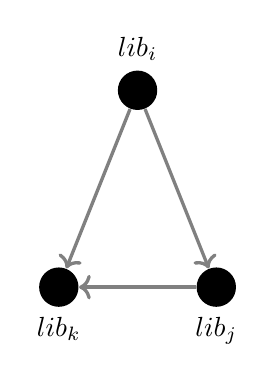
\begin{tikzpicture}[
         roundnode/.style={circle, fill=black, minimum size=5mm},
        squarenode/.style={fill=black, text=red, minimum size=5mm},
     ]
    \begin{scope}
         \node[roundnode, label=above:$lib_i$] (s2_proji) at (3, 2.5) {};
        \node[roundnode, label=below:$lib_j$] (s2_projj) at (4,0) {};
         \node[roundnode, label=below:$lib_k$] (s2_projk) at (2,0) {};
     \end{scope}

     \begin{scope} [every edge/.style={draw=gray, very thick}]
         \path [->] (s2_proji) edge (s2_projj);
         \path [->] (s2_proji) edge (s2_projk);
         \path [->] (s2_projj) edge (s2_projk);
     \end{scope}
     \end{tikzpicture}
    
     \caption{Example dependency graph for a given time period}
     \label{fig:lib}
     \vspace{2ex}
 \end{figure}
\begin{figure}[t]
    \centering

    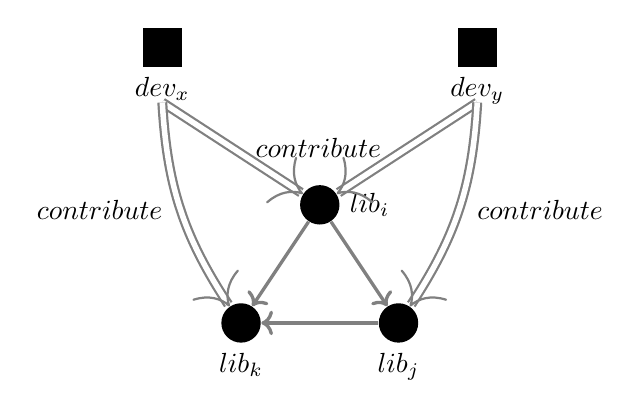
\begin{tikzpicture}[
        roundnode/.style={circle, fill=black, minimum size=5mm},
        squarenode/.style={fill=black, text=red, minimum size=5mm},
    ]
    \begin{scope}
        
        \node[roundnode, label=right:$lib_i$] (s2_proji) at (4, 1.5) {};
        \node[roundnode, label=below:$lib_j$] (s2_projj) at (5,0) {};
        \node[roundnode, label=below:$lib_k$] (s2_projk) at (3,0) {};
        
        \node[squarenode, label=below:$dev_x$] (s3_devx) at (2, 3.5) {};
        
        \node[squarenode, label=below:$dev_y$] (s3_devy) at (6, 3.5) {};
        
    \end{scope}

    \begin{scope} [every edge/.style={draw=gray, very thick}]
        \path [->] (s2_proji)  edge  (s2_projj);
        \path [->] (s2_proji) edge (s2_projk);
        \path [->] (s2_projj) edge (s2_projk);
        
    \end{scope}
    \begin{scope} [every edge/.style={draw=gray, thick, double distance=2pt}]
        \path [->] (6, 2.8) edge node[left = 2mm] {$contribute$} (s2_proji);
        \path [->] (6, 2.8) edge[bend left=15] node[right = 1mm] {$contribute$} (s2_projj);
        \path [->] (2, 2.8) edge node[right = 2mm] {$$} (s2_proji);
        \path [->] (2, 2.8) edge[bend right=15] node[left = 1mm] {$contribute$} (s2_projk);
    \end{scope}
    \end{tikzpicture}
\end{figure}
\begin{figure}[t]
    \centering
    \begin{tikzpicture}[
        roundnode/.style={circle, fill=black, minimum size=5mm},
        squarenode/.style={fill=black, text=red, minimum size=5mm},
    ]
    \end{tikzpicture}
\caption{Example Dependency-Contribution graph showing relationships between contributions and dependencies}
 \label{fig:dc-graph}
\end{figure}

This is just one example of the type of research that is enabled by access to heterogeneous data related to software package ecosystems.

\smallskip\noindent\textbf{Peril 1.}\textit{
 Developers might use different identifiers when contributing to different parts of a software package ecosystem, e.g., when contributing to different libraries.}\\
 
When modelling using such graphs, there is a threat that contributors may use multiple identifiers (i.e., $c_x$ and $c_y$ are the same contributor).
This is a well-known research problem, and there has been work to merge these accounts, such as \cite{wiese2016mailing}.
GitHub has introduced mechanisms such as two-factor authentication\footnote{\url{https://docs.github.com/en/authentication/securing-your-account-with-two-factor-authentication-2fa/configuring-two-factor-authentication}} to counteract the issue of multiple identifiers.
This is since developers might be less likely to switch accounts if it requires cumbersome authentication.


\smallskip\noindent\textbf{Peril 2.}\textit{
Developers' contributions to software package ecosystems might be interspersed with bot contributions, e.g., automated dependency updates.}\\

The rise of automation and artificial intelligence has led to much work on the integration of automated scheduling (i.e., bots) into software development workflows \cite{Storey2016, Farooq2016, Wessel2018, Erlenhov2019, bot_modify_wf} to name a few. These bots are designed to perform specific tasks within a software package ecosystem. For example, a bot may be programmed to automatically update dependencies, test code changes, or deploy software to production. As an example, the Google APIs repo-automation-bots project lists bots for automated labelling of issues and pull requests, automated approval of pull requests, and triggering releases.\footnote{\url{https://github.com/googleapis/repo-automation-bots}}
Bots perform common maintenance tasks in many software projects and are now commonplace \cite{Beschastnikh2017, Urli2018,BIMAN,bot_or_not}.
Especially with bots such as dependabot (automated pull requests to update configurations to reduce the risk of vulnerability threats),\footnote{\url{https://github.com/dependabot}} more and more automation has caused a lot of noise in the contributions between projects.
There are also bots for communication and documentation \cite{Urli2018, Lin2016, Lebeuf2017a}.

To be able to draw accurate conclusions about what humans are doing in software package ecosystems, researchers should consider distinguishing between bot and human contributions.
It is also important to differentiate this from other contributions \cite{maeprasart2022understanding}.
The research community has responded well, with a wide range of techniques and tools to mitigate this peril \cite{Bodegha2021, golzadeh2022accuracy}.

\smallskip\noindent\textbf{Peril 3.}\textit{
Not all developer activities in software package ecosystems are accessible to the public, e.g., library use in proprietary settings.
}\\

Not all developer activities in software package ecosystems are accessible to the public, e.g., when the boundary between open source and industry is blurred \cite{stol2014inner}, which presents a challenge for researchers who aim to study the development process. This is particularly true in proprietary settings where software development is performed behind closed doors or is open source for a limited time period, thus resulting in the artefacts not permanently being publicly available.
This can make it difficult to understand the broader ecosystem in which a software project is developed.
Proprietary settings may lead to non-standardisation in software development practises. Different software projects may use different management systems and tools, making it difficult to accurately compare and analyse software development activities across various projects. For example, some projects may use communication, documentation, and other management tools not captured on the same platform \cite{montgomery2022alternative}. For example, some projects might use Bugzilla instead of issues and pull requests for their bug and code review systems, while others may use Discord, Slack channels, or email threads for their communication needs.

This lack of standardisation in software development practises presents a challenge for researchers who study the software package ecosystem and understand the development process. To address this issue, researchers should strive to collect data from a diverse set of projects to gain a comprehensive understanding of the software package ecosystem. In addition, researchers may need to adjust their methodologies or data collection techniques to accommodate the different tools and practises used by different software projects.

\subsection{Defining Components and their Dependencies}

\smallskip\noindent\textbf{Promise 2.}\textit{
Researchers can access a software package ecosystem's dependency network through package managers and registries, e.g., npm lists the dependencies and dependents for over a million libraries.}\\


With the rise of curated datasets like libraries.io, researchers can now recover and model dependency relations between software units using pre-extracted datasets.
Table \ref{tab:PM_features} shows examples of popular package managers mined from the libraries.io dataset in 2020. 

\begin{table*}[]
\caption{Summary of 13 package managers from libraries.io as ranked by TIOBE in 2020}
 \label{tab:PM_features}
 \centering
\begin{tabular}{@{}llrlll@{}}
\toprule
\begin{tabular}[c]{@{}l@{}}Package \\ Ecosystem\end{tabular} & \begin{tabular}[c]{@{}l@{}}Programming \\ Language\end{tabular} &  \begin{tabular}[c]{@{}l@{}}Tiobe \\ Rank\end{tabular} & Environment & \begin{tabular}[c]{@{}l@{}}Dependency \\ Tree\end{tabular} & \begin{tabular}[c]{@{}l@{}}Package   \\Archive link\end{tabular}\\ \midrule
PyPI & Python & 2 & Python & Flat & pypi.org  \\
Maven & Java & 3 & JVM & Flat & Maven.org  \\
Bower & JavaScript & 7 & Node.js & Flat & bower.io  \\
Meteor & JavaScript & 7 & Node.js & Nested & atmospherejs.com \\
npm & JavaScript & 7 & Node.js & Nested (v2) & npmjs.com  \\
Packagist & PHP & 8 & PHP & Flat & packagist.org \\
Puppet & Ruby & 13 & Ruby MRI & Flat & forge.puppet.com  \\
RubyGems & Ruby & 13 & Ruby MRI & Flat & rubygems.org  \\
CRAN & R & 14 & RStudio & Flat & cran.r-project.org  \\
CPAN & Perl & 15 & Perl & Flat & metacpan.org  \\
GO & Golang & 20 & Go & Flat & pkg.go.dev  \\
NuGet & C\#, VB & 5, 6 & .NET & Flat & nuget.org \\
Anaconda & Python, R, C\# & 2, 14, 5 & Anaconda & Flat & anaconda.org  \\ \bottomrule
\end{tabular}
\end{table*}

\smallskip\noindent\textbf{Peril 4.}\textit{
Different software package ecosystems define the concept of ``dependency'' differently, e.g., by allowing or not allowing different versions of a library on the same dependency tree.
}\\

Different software package ecosystems have varying definitions of what constitutes a dependency. For example, some ecosystems may allow multiple versions of a library to exist on the same dependency tree, while others may restrict developers to a single version of a library \cite{Islam}. These restrictions are often based on the programming language being used, as different languages have different approaches to managing dependencies. It is important to consider the restrictions on dependency relationships when studying software package ecosystems, as they can have a major impact on the development process. For example, the ability to use multiple versions of a library on the same dependency tree can greatly simplify the process of updating dependencies and can make it easier to resolve conflicts between libraries.

One way to visualise the impact of these restrictions is to compare the difference between a nested dependency tree and a directed dependency tree, as shown in Figure \ref{fig:nest}.\footnote{Taken from \url{https://npm.github.io/how-npm-works-docs/npm3/how-npm3-works.html}} This distinction is important because it highlights the different ways that a software unit can depend on different versions of the same library.
In this example, npm v3 creates the dependency tree based on the installation order, therefore flattening unnecessary nested dependencies (i.e., B v1.0 in cyan). This reduces the complexity of a nested tree by resolving some of the transitive dependencies (nested dependencies).

\begin{figure}
	\centering
	\includegraphics[width=.8\textwidth]{book/chapter-promisesandperils/pics/nestedv2.jpg}
	\caption{Difference between flat and nested dependencies}
	\label{fig:nest}
\end{figure}

\smallskip\noindent\textbf{Peril 5.}\textit{
Developers might declare a dependency to other parts of a software package ecosystem but not use it, e.g., because they failed to update its removal.
}\\

It is common for developers to declare dependencies on other parts of the software package ecosystem but not always use them. This can happen for various reasons, such as forgetting to remove the dependency after it is no longer needed. This can pose a challenge for researchers who are trying to extract dependencies from package managers, like those in configuration files, as there may be inconsistencies between the listed dependencies and what is actually being compiled and used by the code. This can lead to a biased understanding of the software package ecosystem and the relationships between software components.

To address this issue, there have been numerous efforts to track the actual library dependencies compiled and executed in software systems. These efforts aim to provide a more accurate understanding of the dependencies and the relationships between software components. For example, research has been conducted on the use of dynamic analysis to track compiled dependencies in real time and on the development of tools to automatically detect and track executed dependencies \cite{Zapata:ICSME2018, Ponta2018,Chinthanet:ASE2020}.

\subsection{Defining Boundaries and Completeness}

\smallskip\noindent\textbf{Promise 3.}\textit{
Researchers can use the boundaries of software package ecosystems to study communities of developers, e.g., developers contributing to and/or benefiting from the npm ecosystem.
}\\

Following Promise 2, the emergence of package managers has also led to studies that approximate software communities.
Using the libraries.io dataset, researchers were able to study projects that host libraries that use package managers.
Researchers have used this dataset to compare different library ecosystems \cite{kikas.2017,decan:emse:2019,CogoDown2019}.


\smallskip\noindent\textbf{Peril 6.}\textit{
Package managers do not always represent software package ecosystems, their communities, or their sub-communities, e.g., in cases where multiple package managers exist.
}\\

Package managers are a fundamental aspect of software package ecosystems, but do not always fully represent the complex relationships and interactions that occur within a community of developers and users, as shown in Table~\ref{tab:PM_features}. In some cases, multiple package managers exist for the same programming language, creating a complex landscape of software libraries and dependencies that are not always easily understood. For instance, Bower and Meteor manage npm libraries, which can lead to confusion and overlap in the management of dependencies.

Similarly, Java, Scala, Android, and other Java-based open source communities all use the Maven package manager, but each of these communities has its own unique set of libraries, dependencies, and development practises. Researchers should be aware of the limitations of package managers when studying software package ecosystems, and consider the broader context and relationships that exist within these communities. 

\smallskip\noindent\textbf{Peril 7.}\textit{
Lack of activity in parts of a software package ecosystem does not necessarily indicate project failure, e.g., when highly depended-upon libraries are feature-complete.
}\\

It is important to note that lack of activity in a part of a software package ecosystem does not always mean project failure \cite{coelho2017modern}. In some cases, highly relied-upon libraries that have reached feature-completeness may see little activity, but continue to be used by the software community. 

However, it is still important to consider the long-term sustainability of these libraries, especially given the rate at which technology and software development practises change. This has become a topic of interest in recent years, and researchers have explored best practises for sustaining open source projects and ensuring their continued success \cite{Ait2022,valiev2018ecosystem}. Understanding the factors that contribute to project sustainability is important to ensure the longevity and continued growth of software package ecosystems.

\smallskip\noindent\textbf{Peril 8.}\textit{
Sampling from a software package ecosystem is challenging since sub-setting might alter the dependency network, e.g., by breaking dependency chains.
}\\

Sampling from a package ecosystem is not straightforward, as the sample composition can be significantly affected due to missing dependency links between libraries. For instance, a subset of the ecosystem might alter the dependencies between libraries, leading to the breakdown of the dependency chains. This could lead to an incomplete picture of the software package ecosystem, leading to incorrect conclusions from a study. To minimise this risk, researchers should carefully consider the boundaries of their study and choose the appropriate sampling method based on the research questions and goals. For example, researchers could focus on popular, highly dependent, or risk-vulnerable aspects of the ecosystem as a starting point. 
For some ecosystems, the number of downloads, GitHub stars, and watchers are other aspects for the researcher to utilise.


\smallskip\noindent\textbf{Peril 9.}\textit{
Sampling from a software package ecosystem is challenging since the dependency network changes over time, e.g., when dependencies are added, removed, upgraded, or downgraded.
}\\

The dynamic nature of package ecosystems and the constant changes to their dependencies can impact the generalisability of the results. Therefore, it is important to also consider the time granularity of the analysis. For example, if the goal is to understand the evolution of dependencies over time, a finer time granularity may be necessary to capture the smaller changes and trends. However, if the goal is to understand the overall structure and relationships within the ecosystem, a coarser time granularity may be sufficient. Based on recent studies \cite{wattanakriengkrai2022giving,valiev2018ecosystem,Mirsaeedi:icse2020, Brindescu:emse2020, Nassif:icsme2017}, a three-month window seems appropriate for some studies.
Another level of granularity to consider is the size of the component. For instance, there are cases where a single package may contain more than one repository, especially for large library frameworks. 
The granularity also depends on the nature of the ecosystem itself. For instance, researchers should understand whether the ecosystem comprises library packages (e.g., PyPI), plugins (e.g., Eclipse), or is a library distribution (e.g., Android).



\subsection{Analysing and Visualising the Data}

\textbf{Peril 10.}\textit{
Analysing and visualising entire software package ecosystems is challenging due to their size, e.g., in terms of nodes and edges in the network.
}\\

The size of software package ecosystems implies large data sets, which can be overwhelming for tools and algorithms to analyse and display. Therefore, it may be necessary to make choices about the granularity of the data included in the analysis and visualisation. Another alternative is to focus on the most critical parts of the software package ecosystem, such as the high-level structure, highly dependent packages, or parts of the system that pose a risk to security and reliability. 
The key is to strike a balance between detail and simplicity, providing a meaningful representation of the ecosystem while being able to handle the complexity of its size.


\section{Application: When to Apply Which Peril}
\label{PPM:sec:application}

We include a disclaimer stating that not all perils are applicable to every mining situation. To demonstrate the practical application of our perils and their mitigation, we present two case studies that involve mining the software package ecosystem. Each case study has a distinct research objective and focusses on a specific dataset to be mined.

\subsection{Two Case Studies}
Table \ref{tab:cases} presents the two case studies we have selected for this analysis.
The \textit{first case} involves mining for contributions congruent to dependency updates \cite{wattanakriengkrai2022giving}. 
In this work, the authors mine GitHub repositories for Pull Requests and Issues that were submitted and merged congruent to dependency updates within the npm ecosystem. 
The \textit{second case} involves mining communication data for the Eclipse ecosystem \cite{Nugroho2021}. Although the second case does not mine for dependency relations (i.e., use relations),  we show that these perils still apply when mining for other relationships in an ecosystem.
Moreover, the second case studies the Eclipse ecosystem, which is a different dataset compared to the more popular GitHub dataset.

\subsection{Applying Perils and their Mitigation Strategies}
Table \ref{tab:perilsapp} provides a summary of the perils that can be applied to each of the case studies. We will now go into the details of mitigation strategies based on these perils. 
For better organisation and understanding, we have grouped the perils according to the four logical processes for mining.

\smallskip\noindent\textbf{Information to Mine}. 
The first set of mitigation strategies, which addresses perils 1-3, focusses on planning which information to mine. There are two primary strategies that researchers can employ:


\begin{enumerate}
    \item Researchers should use research tools and techniques to remove noise and other biases in the dataset, such as bot detection and the handling of multiple identities. This strategy was implemented in both case studies, as contributions and discussions often have the potential to involve bots or developers with multiple identities.
\item Depending on the research goals, researchers should recognise that not all contributions are equal and filter the dataset accordingly.
\end{enumerate}

We applied these two strategies to both cases. In the first case, the goal was to capture all congruent contributions, so we filtered out contributions made to libraries without dependencies. Since all npm packages are listed in the registry, Peril 3 (private activities) did not apply.
In the second case, we addressed Peril 1 by conducting a qualitative analysis to ensure that the member identities were not duplicated, as Eclipse developers were known to change identities. To mitigate Peril 2, we removed bot responses. For the second case, since all forum data is made public, Peril 3 did not apply.


\begin{table}
\centering
\caption{Description of the research objectives and datasets for the case studies}
 \label{tab:cases}
\begin{tabular}{lp{5cm}r} 
\toprule
\textbf{Case Study} & \textbf{Research Objective}                                                          & \textbf{Datasets}           \\
\midrule
Wattanakriengkrai \etal \cite{wattanakriengkrai2022giving}             & Explore code contributions between library and client (i.e, use-relations)  & libraries.io\\
& &  GitHub API \\
Nugroho \etal \cite{Nugroho2021}                & Explore discussion contributions between contributors (i.e., contributions) & Eclipse API                \\
\bottomrule
\end{tabular}
\end{table}

\begin{table}
\centering
\caption{Application of each peril to the case studies}
 \label{tab:perilsapp}
\begin{tabular}{rp{8cm}ccc} 
\toprule                   
& \textbf{Perils}       & case 1      & case 2                 \\
                                                                               & & npm  & Eclipse   \\
\midrule
\textbf{P1} &Developers might use different identifiers when contributing to different parts of a software package ecosystem, e.g., when contributing to different libraries.                             &    \CheckedBox         &          \CheckedBox           \\ 
%\hline
\textbf{P2} & Developers' contributions to software package ecosystems might be interspersed with bot contributions, e.g., automated dependency updates.                                                      &      \CheckedBox               &      \CheckedBox               \\ 
%\hline
\textbf{P3} & Not all developer activities in software package ecosystems are accessible to the public, e.g., library use in proprietary settings.                                                         &         -           &      \CheckedBox               \\ 
%\hline
\textbf{P4} & Different software package ecosystems define the concept of \`{}\`{}dependency'' differently, e.g., by allowing or not allowing different versions of a library on the same dependency tree. &         \CheckedBox       &     -                            \\ 
%\hline
\textbf{P5} & Developers might declare a dependency to other parts of a software package ecosystem but not use it, e.g., because they failed to update its removal.                                        &     -           &  -    \\
%\hline
\textbf{P6} &Package managers do not always represent software package ecosystems, their communities, or their sub-communities, e.g., in cases where multiple package managers exist.                     &     -                   &  -                  \\
%\hline
\textbf{P7} & Lack of activity in parts of a software package ecosystem does not necessarily indicate project failure, e.g., when highly depended-upon libraries are feature-complete.                     &       \CheckedBox         &  -                           \\
%\hline
\textbf{P8} &Sampling from a software package ecosystem is challenging since sub-setting might alter the dependency network, e.g., by breaking dependency chains.                                         &        \CheckedBox        &     \CheckedBox                                \\
%\hline
\textbf{P9} &Sampling from a software package ecosystem is challenging since the dependency network changes over time, e.g., when dependencies are added, removed, upgraded, or downgraded.               &       \CheckedBox         &     -                          \\
%\hline
\textbf{P10} &Analysing and visualising entire software package ecosystems is challenging due to their size, e.g., in terms of nodes and edges in the network.                                  &        \CheckedBox      &      \CheckedBox               \\
\bottomrule
\end{tabular}
\end{table}

\smallskip\noindent\textbf{Defining Dependencies}. 
The second set of perils (Perils 4-5) is related to dependency relationships between software units, and only the first case study is applicable. To address these perils, researchers should adopt the following strategy:

\begin{enumerate}
    \item Researchers should not rely solely on listed dependencies in configuration files (e.g., pom.xml, package.json, etc.) as a measure of dependency between two components. Instead, code-centric approaches should be used to validate which libraries are actually depended upon.
\end{enumerate}

For example, in the first case, in addition to mining the configuration information, the authors also analysed the similarity of the source code contributions to address Peril 4. Regarding Peril 5, since the study's objective was to investigate changes to the configuration files, the risk of the update not being executed was deemed less important.
It is important to note that the second case study did not include dependency analysis and, therefore, these perils did not apply.

\begin{figure*}[]
    \centering
    \begin{subfigure}{0.9\linewidth}
         \includegraphics[width=1.1\textwidth]{book/chapter-promisesandperils/pics/congruentViz.jpg}
         \caption{Visualization of a Time analysis for 107,242 libraries.}
     \end{subfigure}
     \begin{subfigure}{0.9\linewidth}
         \includegraphics[width=1\textwidth]{book/chapter-promisesandperils/pics/eclipseViz.jpg}
         \caption{A Visual Topology map for 832,058 threads}
     \end{subfigure}
    \caption{Visualisation examples for the two case studies}
    \label{fig:visCase}
\end{figure*}

\smallskip\noindent\textbf{Defining Boundaries}.
The third set of perils (Perils 6-9) is related to the definition of boundaries and completeness and is relevant for both case studies. To mitigate these perils, we recommend the following strategies:

\begin{enumerate}
    \item Researchers should recognise that a dormant project does not necessarily mean that it is inactive. Instead, studies can use alternative heuristics, such as the number of dependents and dependencies, as better indicators of a project's importance in the ecosystem.
    \item Researchers should not rely solely on the programming language to define sub-communities. Using a common package manager for the programming language is a more effective rule of thumb for distinguishing boundaries.
    \item Researchers should avoid random sampling. Instead, sampling should be tailored to the research goals by considering factors such as an appropriate time window or focussing on specific attributes of components (e.g., most dependents, most popular, most contributors).
\end{enumerate}


Peril 6 did not apply to any of the case studies. 
Particularly for the first case, since the goal was to explore the npm package ecosystem, we assumed that the boundaries were clearly defined by the npm registry. 
Similarly, the second case study used the generic Eclipse platform as the boundary. 
Peril 7 was applied to the npm study, while Peril 8 was applied to both case studies. 
As a result, the two cases conducted a qualitative analysis of the dataset to gain deeper insights.
In the first case study, a three-month time window was created to capture dependencies. 
For the second case study, forum contributors were sampled into three groups (i.e., junior, member, or senior) according to the sliding window of their contributions. 

\smallskip\noindent\textbf{Visualisation}.
The final peril (Peril 10) relates to visualisation, which can be challenging due to the vast size and complexity of software ecosystems. As it is not feasible to visualise every aspect of an ecosystem simultaneously, a focused approach is necessary. A mitigation strategy is to select specific attributes of the ecosystem (e.g., the most dependent, most popular, and most contributions) that align with the research needs and objectives. 

Figure \ref{fig:visCase} shows two cases where visualizations are employed to gain insights, especially for large datasets.
In the first figure (a), we visualize the distributions of the data set and applied the appropriate statistical tests, along with the effect size, to test our hypotheses and answer research questions. 
In the second example (b), although not directly related to package ecosystems, the authors utilized a topological visualization \cite{Lum2013ExtractingIF} to gain insights on the over 800,000 forum threads of discussions. 



\section{Chapter Summary}
In this chapter, we explore the various aspects of mining information from the software package ecosystem, presenting three promises and ten perils that researchers should be aware of when undertaking such tasks. The chapter is structured around four key processes for mining: 1) Planning what Information to Mine, 2) Defining Components and their Dependencies, 3) Defining Boundaries and Completeness, and 4) Analysing and Visualising the Data. To help new and experienced researchers navigate these challenges, we introduced the SUG model, which can serve as a valuable tool to minimise threats to validity. Although some perils may be more relevant to specific research objectives, our aim is to equip researchers with the knowledge and resources needed to confidently gather and integrate software package ecosystem data into their work.

% %Semantic labeling three-letter-code: FRK (e.g. \chapter{FRK})

% 
\title{Promises and Perils of Mining \\ Software Package Ecosystem Data}
\author{Raula Gaikovina Kula \and Katsuro Inoue \and Christoph Treude}
\institute{Raula Gaikovina Kula \at Nara Institute of Science and Technology, Japan, \email{raula-k@naist.jp}
\and Katsuro Inoue \at Nanzan University, Japan \email{ inoue599@nanzan-u.ac.jp}
\and  Christoph Treude \at The University of Melbourne, Australia \email{christoph.treude@unimelb.edu.au}}

\maketitle
\label{PPM:ch}
\abstract*{The use of third-party packages is becoming increasingly popular and has led to the emergence of large software package ecosystems with a maze of inter-dependencies. Since the reliance on these ecosystems enables developers to reduce development effort and increase productivity, it has attracted the interest of researchers: understanding the infrastructure and dynamics of package ecosystems has given rise to approaches for better code reuse, automated updates, and the avoidance of vulnerabilities, to name a few examples. But the reality of these ecosystems also poses challenges to software engineering researchers, such as: How do we obtain the complete network of dependencies along with the corresponding versioning information? What are the boundaries of these package ecosystem? How do we consistently detect dependencies that are declared but not used? How do we consistently identify developers within a package ecosystem? How much of the ecosystem do we need to understand to analyse a single component? How well do our approaches generalise across different programming languages and package ecosystems? In this chapter, we review promises and perils of mining the rich data related to software package ecosystems available to software engineering researchers.}

\abstract{The use of third-party packages is becoming increasingly popular and has led to the emergence of large software package ecosystems with a maze of inter-dependencies. Since the reliance on these ecosystems enables developers to reduce development effort and increase productivity, it has attracted the interest of researchers: understanding the infrastructure and dynamics of package ecosystems has given rise to approaches for better code reuse, automated updates, and the avoidance of vulnerabilities, to name a few examples. But the reality of these ecosystems also poses challenges to software engineering researchers, such as: How do we obtain the complete network of dependencies along with the corresponding versioning information? What are the boundaries of these package ecosystems? How do we consistently detect dependencies that are declared but not used? How do we consistently identify developers within a package ecosystem? How much of the ecosystem do we need to understand to analyse a single component? How well do our approaches generalise across different programming languages and package ecosystems? In this chapter, we review promises and perils of mining the rich data related to software package ecosystems available to software engineering researchers.}

%%%%%%%%%%%%%%%%%%%%%%%%%%%%%%%%%%%%%%%%%%%%%%%%%%%%%%%%%%%%%%%%%%

\section{Introduction}
\label{PPM:sec:definition}

Third-party libraries are a great way for developers to incorporate code without having to write their own for every functionality required. By using these libraries, developers can save time and energy while still getting the functions they need.
Using third-party libraries is becoming increasingly popular and has led to the emergence of large software package ecosystems such as npm. While these ecosystems offer many benefits, they also come with risks, such as software vulnerability attacks \cite{Chinthanet:ASE2020}.

Large software package ecosystems are a treasure trove for researchers who can investigate a wide range of questions. For example, by studying activity in large ecosystems, researchers can identify which libraries are the most popular and learn what characteristics make them successful \cite{kikas.2017,decan:emse:2019}.
Additionally, research on large ecosystems can help developers understand how to protect their code from malicious actors who may attempt to exploit vulnerabilities or insert malware into popular libraries.
Studying large software package ecosystems can help us better understand the dynamics of open source development in general. Open source development is a complex process that involves many different stakeholders working together (or sometimes competing) to create valuable code that anyone can use or improve upon. By understanding how these interactions play out in different types of ecosystem structures -- including those with many small projects versus few very large ones -- we can develop insights that might be applicable more broadly across other types of collaborative systems.

In this chapter, we identify and discuss promises and perils during the mining process, ranging from planning what information to mine from the ecosystem to analysing and visualising the mined data. 
Therefore, the chapter is broken down into these logical processes of mining ecosystem data: 1) Planning what Information to Mine, 2) Defining Components and their Dependencies, 3) Defining Boundaries and Completeness, and 4) Analysing and Visualising the Data.

This chapter is intended for researchers and practitioners who are interested in exploring and exploiting software package ecosystem information from a diverse range of sources that are publicly available. 
We also highlight the pitfalls to consider during the mining process, particularly when these pitfalls could lead to a misinterpretation of the analysis and results. 
The chapter is written in a manner that encourages newcomers who have little or no experience or who are interested in utilising ecosystem data across different disciplines outside of software engineering.
Our goal is to get new researchers quickly accustomed to gathering ecosystem information for their research.


\section{A Component-based Software Ecosystem}

Defined as a component-based software ecosystem, we suggest using the term `software package ecosystem' as a suitable term for the symbiotic relationships among third-party library components (as software projects or repositories), as these libraries and their dependent clients coexist on the same technological platform, therefore sharing the same environment and other internal and external factors (e.g., security threats, sharing contributions, etc.).
Please refer to the Introduction chapter for an in-depth definition of the different types of software ecosystems.
We present our interpretation of the software package ecosystem in Kula et al.~\cite{KulaSANER18}, where we formally define a package ecosystem using a Software Universe Graph (SUG).
This is modelled as a structured abstraction of the evolution of software systems and their library dependencies over time.

%%%%%%%%%%%%%%%%%%%%%%%%%%%%%%%%%%%%%%%%%%
\begin{figure*}
	\centering
	\includegraphics[width=.7\textwidth]{book/chapter-promisesandperils/pics/UniversalExample.jpg}
	\caption{Conceptual example of the Software Universe Graph, depicting the use and update relationships between different software units.}
	\label{fig:SUG}
\end{figure*}
%%%%%%%%%%%%%%%%%%%%%%%%%%%%%%%%%%%%%%%%%%%%%


\paragraph{\textbf{Component-based Representation as a Software Universe Graph}}
\label{PPM:sec:SUG}

First introduced by Kula et al.~\cite{KulaSANER18}, the \textit{Software Universe Graph} (SUG) is a structural abstraction of the software ecosystem of third-party libraries.
Figure \ref{fig:SUG} provides an illustration of the different relationships within the graph.
Let $G= (N,E)$ represent a graph $G$. $N$ is a set of nodes, each node representing a software unit. 
We define a software unit as a version instance of any software program. 

The authors then present the \textit{use} and \textit{update} relationships that exist in the ecosystem.
Hence, the edges $E$ are composed of $E_{use}$ and $E_{update}$. $E_{use}$ is a set of \textit{use-relations} and $E_{update}$ is a set of \textit{update-relations}.

\begin{definition}
An edge $u \rightarrow v \in E_{use}$ means that $u$ uses $v$. The defined functions of $E_{use}$ are:

\begin{equation}
\small
\small \use(u)\equiv \{v|u \rightarrow v\}
\normalsize
\end{equation}
\begin{equation}
\small
\small \useBy(u)\equiv \{v|v \rightarrow u\}
\normalsize
\end{equation}
\end{definition}

Use-relations can be extracted from either the source code or configuration files. 
As shown in Figure \ref{fig:SUG}, node $a1$ uses node $x1$. 
In addition, node $x1$ is used by nodes $a1$, $q1$, and $q2$. Parallel edges for node pairs are not allowed.

\begin{definition}
We represent an update relation from node $a$ to $b$ using $ a \Rightarrow b $, which means that the newer update $b$ was released from node $a$ and is defined as:
\begin{equation}
\small a \Rightarrow b \in E_{update}
\end{equation}
\end{definition}

Update relations refer to when a successive release of a software unit is made available. Figure \ref{fig:SUG} shows that node $q1$ is first updated to node $q2$. Later, node $q2$ is updated to the latest node $q3$. Hence, $q1 \Rightarrow q2 \Rightarrow q3$.
Note that an update should not be confused with forking. 
We distinguish a fork as a separate software unit. 
Each node in the SUG should be denoted by three attributes: \texttt{<name,release,time>}.  
For a node $u$, we define:

\begin{itemize}
	\item \textbf{u.name} Name is the string representation identifier of a software unit.
	We introduce the name axiom: For nodes $u$ and $v$, if $u \Rightarrow v$, then $u.name = v.name$ holds.
	
	\item \textbf{u.release}. Release refers to the specific assigned change reference for a software unit. For nodes $u$ and $v$, if $u \Rightarrow v$
	then $v$ is the immediate successor of $u$. Note that the versioning pattern may vary from project to project. 
	\item \textbf{u.time}. Time refers to the time stamp at which node $u$ was released. For nodes $u$ and $v$ of $u \Rightarrow v$, $u.time < v.time$.
\end{itemize}

\begin{figure}
	\centering
	\includegraphics[width=.8\textwidth]{book/chapter-promisesandperils/pics/TemporalSUG.jpg}
	\caption{Temporal property of the SUG}
	\label{fig:SUGTemp}
\end{figure}

\begin{definition}
    
	The SUG has temporal properties.
This describes the simultaneity or ordering in reference to time. Let SUG $G = (N, E) $ be at time $t$. At time $t^{\prime} > t$, we observe an extension of $G$, such that:

\begin{equation}
\small G^{\prime} = (N \cup \Delta N, E \cup \Delta E)
\end{equation}
where $\Delta E \cap (N \times N) = \emptyset$
\end{definition}

Figure \ref{fig:SUGTemp} illustrates the temporal properties of the SUG. 
Here, it is observed that $G'$ is composed of $G$ augmented with newly added node $a3$ and its corresponding $a3 \rightarrow x2$ and $a2 \Rightarrow a3$ relations.
A SUG grows monotonically over time with only additions.
Here, we consider that modification or deletion changes on the SUG do not occur. 

\begin{definition}
    A timed SUG specifies the state of the SUG at any point in time.
So for an SUG $G=(N,E)$, we represent a timed SUG $G_{t}$ at time $t$ as a sub-graph of $G$. Formally,
\begin{equation}
\small G_t\equiv(N_{t}, E_{t})
\end{equation}
where $N_{t} = \{u|u \in N, u.time \leq t \}$ and $E_t = \{ e | e \in E \wedge e \in  N_t \}$
\end{definition}
	


\section{Data Sources}
Researchers can use various datasets to model the ecosystem using the SUG model of usage and update relationships.
The most obvious data source that has revolutionised data mining in the software engineering domain is the GitHub platform. 
Established in 2008, and then purchased by Microsoft in 2020, GitHub is home to various popular Open Source Software. 
GitHub is built on the git version control system and is useful for storing all changes made to a repository. 
In the case of the SUG, a GitHub repository can represent one software unit, whose depend relations can be extracted via a configuration file (such as the package.json file for JavaScript projects).
The repository should also contain the release information that holds the update relations.
Due to its large size, researchers and the GitHub team have made available datasets for researchers to mine, for example through the GitHub API/Graph QL.\footnote{\url{https://docs.github.com/en/graphql}} This is the backend Application Programming Interface (API) that can be used to query large amounts of data on GitHub. Most researchers use the API to download and mine information from the GitHub platform. 
It is important to note that while GitHub introduced a new feature of Dependency Graphs to map the depend relationship,\footnote{\url{https://docs.github.com/en/code-security/supply-chain-security/understanding-your-software-supply-chain/about-the-dependency-graph}} most older projects do not have this feature.
In this case, the researcher would need to manually extract and query the configuration files for dependency information. 

We refer to the first chapter for additional information on data sources for mining software ecosystems. 

\section{Promises and Perils}
\label{PPM:sec:promisesperils}

Using the SUG model of depend and use relations and the available datasets, we can now present our promises and perils of mining ecosystem information.

\subsection{Planning What Information to Mine}

\textbf{Promise 1.}\textit{
Researchers can access and link heterogeneous data related to software package ecosystems, e.g., package registries and bug trackers.}\\

When planning what information to mine from the ecosystem, researchers do not need to limit themselves to the usage and update relationship information.
Platforms that host software repositories include other software management systems such as bug trackers.
For example, GitHub allows researchers to manage GitHub Pull Requests, Issues, and Discussions not only for one project, but for multiple projects.
GitHub provides three management systems that are related to a software repository:

\begin{itemize}
    \item \textit{GitHub Discussions}\footnote{\url{https://docs.github.com/en/discussions}} - The GitHub Discussions forum is a collaborative communication forum for the community around an open source or internal project. Community members can ask and answer questions, share updates, have open-ended conversations, and follow along on decisions affecting the community's way of working.
    \item \textit{GitHub Pull Requests}\footnote{\url{https://docs.github.com/en/pull-requests}} - Pull Requests allow other developers from an ecosystem to make a contribution to a software repository. Pull requests also allow maintainers to discuss and review potential changes with collaborators and add follow-up commits before changes are merged into the software.
    \item \textit{GitHub Issues}\footnote{\url{https://docs.github.com/en/issues}} - Issues are used to track ideas, feedback, tasks, or bugs for work on GitHub.
\end{itemize}

These three systems are examples of how developers contribute to both their own and other projects. 
Hence, to incorporate this information, we can extend the SUG model, creating a model that includes a contribution relationship \cite{wattanakriengkrai2022giving}.

% Note that other platforms may also have management systems, like GitLab, BitBucket and Eclipse.

\begin{definition}
	A Dependency-Contribution graph incorporates contributions by developers whose libraries are involved in dependency relationships. 
\end{definition}

In this work \cite{wattanakriengkrai2022giving}, the authors explore the congruence between dependency updates and developer contributions, based on the original concept of social-technical congruence \cite{stcCataldo2008} where developers contribution patterns are congruent with their coordination needs. Hence, the goal is to identify contributions that are congruent to dependency updates.
As shown in Figure \ref{fig:lib} the authors extend from the typical SUG graph model where $lib_i$ depends (use) on  $lib_k$ and  $lib_j$, while  $lib_j$ also depends on $lib_k$, to the example shown in Figure \ref{fig:dc-graph}.
Different to the SUG, the graph captures developers and their contributions (i.e., the square as $dev_x$ and $dev_y$ represent two different developers making a contribution).
Here contributions are defined as $c$ (Pull Request or Issue) that were submitted to both a library and the client that depends on that library.
Hence, the graph can show contributions that are congruent to dependency changes for a software unit. 

\begin{figure}[t]
     \centering
     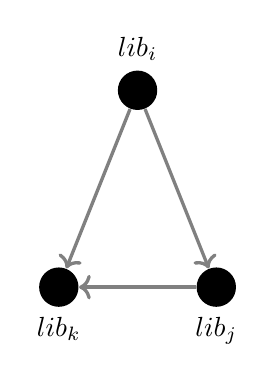
\begin{tikzpicture}[
         roundnode/.style={circle, fill=black, minimum size=5mm},
        squarenode/.style={fill=black, text=red, minimum size=5mm},
     ]
    \begin{scope}
         \node[roundnode, label=above:$lib_i$] (s2_proji) at (3, 2.5) {};
        \node[roundnode, label=below:$lib_j$] (s2_projj) at (4,0) {};
         \node[roundnode, label=below:$lib_k$] (s2_projk) at (2,0) {};
     \end{scope}

     \begin{scope} [every edge/.style={draw=gray, very thick}]
         \path [->] (s2_proji) edge (s2_projj);
         \path [->] (s2_proji) edge (s2_projk);
         \path [->] (s2_projj) edge (s2_projk);
     \end{scope}
     \end{tikzpicture}
    
     \caption{Example dependency graph for a given time period}
     \label{fig:lib}
     \vspace{2ex}
 \end{figure}
\begin{figure}[t]
    \centering

    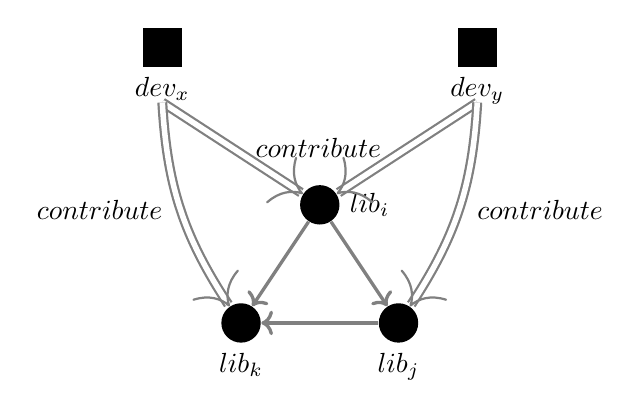
\begin{tikzpicture}[
        roundnode/.style={circle, fill=black, minimum size=5mm},
        squarenode/.style={fill=black, text=red, minimum size=5mm},
    ]
    \begin{scope}
        
        \node[roundnode, label=right:$lib_i$] (s2_proji) at (4, 1.5) {};
        \node[roundnode, label=below:$lib_j$] (s2_projj) at (5,0) {};
        \node[roundnode, label=below:$lib_k$] (s2_projk) at (3,0) {};
        
        \node[squarenode, label=below:$dev_x$] (s3_devx) at (2, 3.5) {};
        
        \node[squarenode, label=below:$dev_y$] (s3_devy) at (6, 3.5) {};
        
    \end{scope}

    \begin{scope} [every edge/.style={draw=gray, very thick}]
        \path [->] (s2_proji)  edge  (s2_projj);
        \path [->] (s2_proji) edge (s2_projk);
        \path [->] (s2_projj) edge (s2_projk);
        
    \end{scope}
    \begin{scope} [every edge/.style={draw=gray, thick, double distance=2pt}]
        \path [->] (6, 2.8) edge node[left = 2mm] {$contribute$} (s2_proji);
        \path [->] (6, 2.8) edge[bend left=15] node[right = 1mm] {$contribute$} (s2_projj);
        \path [->] (2, 2.8) edge node[right = 2mm] {$$} (s2_proji);
        \path [->] (2, 2.8) edge[bend right=15] node[left = 1mm] {$contribute$} (s2_projk);
    \end{scope}
    \end{tikzpicture}
\end{figure}
\begin{figure}[t]
    \centering
    \begin{tikzpicture}[
        roundnode/.style={circle, fill=black, minimum size=5mm},
        squarenode/.style={fill=black, text=red, minimum size=5mm},
    ]
    \end{tikzpicture}
\caption{Example Dependency-Contribution graph showing relationships between contributions and dependencies}
 \label{fig:dc-graph}
\end{figure}

This is just one example of the type of research that is enabled by access to heterogeneous data related to software package ecosystems.

\smallskip\noindent\textbf{Peril 1.}\textit{
 Developers might use different identifiers when contributing to different parts of a software package ecosystem, e.g., when contributing to different libraries.}\\
 
When modelling using such graphs, there is a threat that contributors may use multiple identifiers (i.e., $c_x$ and $c_y$ are the same contributor).
This is a well-known research problem, and there has been work to merge these accounts, such as \cite{wiese2016mailing}.
GitHub has introduced mechanisms such as two-factor authentication\footnote{\url{https://docs.github.com/en/authentication/securing-your-account-with-two-factor-authentication-2fa/configuring-two-factor-authentication}} to counteract the issue of multiple identifiers.
This is since developers might be less likely to switch accounts if it requires cumbersome authentication.


\smallskip\noindent\textbf{Peril 2.}\textit{
Developers' contributions to software package ecosystems might be interspersed with bot contributions, e.g., automated dependency updates.}\\

The rise of automation and artificial intelligence has led to much work on the integration of automated scheduling (i.e., bots) into software development workflows \cite{Storey2016, Farooq2016, Wessel2018, Erlenhov2019, bot_modify_wf} to name a few. These bots are designed to perform specific tasks within a software package ecosystem. For example, a bot may be programmed to automatically update dependencies, test code changes, or deploy software to production. As an example, the Google APIs repo-automation-bots project lists bots for automated labelling of issues and pull requests, automated approval of pull requests, and triggering releases.\footnote{\url{https://github.com/googleapis/repo-automation-bots}}
Bots perform common maintenance tasks in many software projects and are now commonplace \cite{Beschastnikh2017, Urli2018,BIMAN,bot_or_not}.
Especially with bots such as dependabot (automated pull requests to update configurations to reduce the risk of vulnerability threats),\footnote{\url{https://github.com/dependabot}} more and more automation has caused a lot of noise in the contributions between projects.
There are also bots for communication and documentation \cite{Urli2018, Lin2016, Lebeuf2017a}.

To be able to draw accurate conclusions about what humans are doing in software package ecosystems, researchers should consider distinguishing between bot and human contributions.
It is also important to differentiate this from other contributions \cite{maeprasart2022understanding}.
The research community has responded well, with a wide range of techniques and tools to mitigate this peril \cite{Bodegha2021, golzadeh2022accuracy}.

\smallskip\noindent\textbf{Peril 3.}\textit{
Not all developer activities in software package ecosystems are accessible to the public, e.g., library use in proprietary settings.
}\\

Not all developer activities in software package ecosystems are accessible to the public, e.g., when the boundary between open source and industry is blurred \cite{stol2014inner}, which presents a challenge for researchers who aim to study the development process. This is particularly true in proprietary settings where software development is performed behind closed doors or is open source for a limited time period, thus resulting in the artefacts not permanently being publicly available.
This can make it difficult to understand the broader ecosystem in which a software project is developed.
Proprietary settings may lead to non-standardisation in software development practises. Different software projects may use different management systems and tools, making it difficult to accurately compare and analyse software development activities across various projects. For example, some projects may use communication, documentation, and other management tools not captured on the same platform \cite{montgomery2022alternative}. For example, some projects might use Bugzilla instead of issues and pull requests for their bug and code review systems, while others may use Discord, Slack channels, or email threads for their communication needs.

This lack of standardisation in software development practises presents a challenge for researchers who study the software package ecosystem and understand the development process. To address this issue, researchers should strive to collect data from a diverse set of projects to gain a comprehensive understanding of the software package ecosystem. In addition, researchers may need to adjust their methodologies or data collection techniques to accommodate the different tools and practises used by different software projects.

\subsection{Defining Components and their Dependencies}

\smallskip\noindent\textbf{Promise 2.}\textit{
Researchers can access a software package ecosystem's dependency network through package managers and registries, e.g., npm lists the dependencies and dependents for over a million libraries.}\\


With the rise of curated datasets like libraries.io, researchers can now recover and model dependency relations between software units using pre-extracted datasets.
Table \ref{tab:PM_features} shows examples of popular package managers mined from the libraries.io dataset in 2020. 

\begin{table*}[]
\caption{Summary of 13 package managers from libraries.io as ranked by TIOBE in 2020}
 \label{tab:PM_features}
 \centering
\begin{tabular}{@{}llrlll@{}}
\toprule
\begin{tabular}[c]{@{}l@{}}Package \\ Ecosystem\end{tabular} & \begin{tabular}[c]{@{}l@{}}Programming \\ Language\end{tabular} &  \begin{tabular}[c]{@{}l@{}}Tiobe \\ Rank\end{tabular} & Environment & \begin{tabular}[c]{@{}l@{}}Dependency \\ Tree\end{tabular} & \begin{tabular}[c]{@{}l@{}}Package   \\Archive link\end{tabular}\\ \midrule
PyPI & Python & 2 & Python & Flat & pypi.org  \\
Maven & Java & 3 & JVM & Flat & Maven.org  \\
Bower & JavaScript & 7 & Node.js & Flat & bower.io  \\
Meteor & JavaScript & 7 & Node.js & Nested & atmospherejs.com \\
npm & JavaScript & 7 & Node.js & Nested (v2) & npmjs.com  \\
Packagist & PHP & 8 & PHP & Flat & packagist.org \\
Puppet & Ruby & 13 & Ruby MRI & Flat & forge.puppet.com  \\
RubyGems & Ruby & 13 & Ruby MRI & Flat & rubygems.org  \\
CRAN & R & 14 & RStudio & Flat & cran.r-project.org  \\
CPAN & Perl & 15 & Perl & Flat & metacpan.org  \\
GO & Golang & 20 & Go & Flat & pkg.go.dev  \\
NuGet & C\#, VB & 5, 6 & .NET & Flat & nuget.org \\
Anaconda & Python, R, C\# & 2, 14, 5 & Anaconda & Flat & anaconda.org  \\ \bottomrule
\end{tabular}
\end{table*}

\smallskip\noindent\textbf{Peril 4.}\textit{
Different software package ecosystems define the concept of ``dependency'' differently, e.g., by allowing or not allowing different versions of a library on the same dependency tree.
}\\

Different software package ecosystems have varying definitions of what constitutes a dependency. For example, some ecosystems may allow multiple versions of a library to exist on the same dependency tree, while others may restrict developers to a single version of a library \cite{Islam}. These restrictions are often based on the programming language being used, as different languages have different approaches to managing dependencies. It is important to consider the restrictions on dependency relationships when studying software package ecosystems, as they can have a major impact on the development process. For example, the ability to use multiple versions of a library on the same dependency tree can greatly simplify the process of updating dependencies and can make it easier to resolve conflicts between libraries.

One way to visualise the impact of these restrictions is to compare the difference between a nested dependency tree and a directed dependency tree, as shown in Figure \ref{fig:nest}.\footnote{Taken from \url{https://npm.github.io/how-npm-works-docs/npm3/how-npm3-works.html}} This distinction is important because it highlights the different ways that a software unit can depend on different versions of the same library.
In this example, npm v3 creates the dependency tree based on the installation order, therefore flattening unnecessary nested dependencies (i.e., B v1.0 in cyan). This reduces the complexity of a nested tree by resolving some of the transitive dependencies (nested dependencies).

\begin{figure}
	\centering
	\includegraphics[width=.8\textwidth]{book/chapter-promisesandperils/pics/nestedv2.jpg}
	\caption{Difference between flat and nested dependencies}
	\label{fig:nest}
\end{figure}

\smallskip\noindent\textbf{Peril 5.}\textit{
Developers might declare a dependency to other parts of a software package ecosystem but not use it, e.g., because they failed to update its removal.
}\\

It is common for developers to declare dependencies on other parts of the software package ecosystem but not always use them. This can happen for various reasons, such as forgetting to remove the dependency after it is no longer needed. This can pose a challenge for researchers who are trying to extract dependencies from package managers, like those in configuration files, as there may be inconsistencies between the listed dependencies and what is actually being compiled and used by the code. This can lead to a biased understanding of the software package ecosystem and the relationships between software components.

To address this issue, there have been numerous efforts to track the actual library dependencies compiled and executed in software systems. These efforts aim to provide a more accurate understanding of the dependencies and the relationships between software components. For example, research has been conducted on the use of dynamic analysis to track compiled dependencies in real time and on the development of tools to automatically detect and track executed dependencies \cite{Zapata:ICSME2018, Ponta2018,Chinthanet:ASE2020}.

\subsection{Defining Boundaries and Completeness}

\smallskip\noindent\textbf{Promise 3.}\textit{
Researchers can use the boundaries of software package ecosystems to study communities of developers, e.g., developers contributing to and/or benefiting from the npm ecosystem.
}\\

Following Promise 2, the emergence of package managers has also led to studies that approximate software communities.
Using the libraries.io dataset, researchers were able to study projects that host libraries that use package managers.
Researchers have used this dataset to compare different library ecosystems \cite{kikas.2017,decan:emse:2019,CogoDown2019}.


\smallskip\noindent\textbf{Peril 6.}\textit{
Package managers do not always represent software package ecosystems, their communities, or their sub-communities, e.g., in cases where multiple package managers exist.
}\\

Package managers are a fundamental aspect of software package ecosystems, but do not always fully represent the complex relationships and interactions that occur within a community of developers and users, as shown in Table~\ref{tab:PM_features}. In some cases, multiple package managers exist for the same programming language, creating a complex landscape of software libraries and dependencies that are not always easily understood. For instance, Bower and Meteor manage npm libraries, which can lead to confusion and overlap in the management of dependencies.

Similarly, Java, Scala, Android, and other Java-based open source communities all use the Maven package manager, but each of these communities has its own unique set of libraries, dependencies, and development practises. Researchers should be aware of the limitations of package managers when studying software package ecosystems, and consider the broader context and relationships that exist within these communities. 

\smallskip\noindent\textbf{Peril 7.}\textit{
Lack of activity in parts of a software package ecosystem does not necessarily indicate project failure, e.g., when highly depended-upon libraries are feature-complete.
}\\

It is important to note that lack of activity in a part of a software package ecosystem does not always mean project failure \cite{coelho2017modern}. In some cases, highly relied-upon libraries that have reached feature-completeness may see little activity, but continue to be used by the software community. 

However, it is still important to consider the long-term sustainability of these libraries, especially given the rate at which technology and software development practises change. This has become a topic of interest in recent years, and researchers have explored best practises for sustaining open source projects and ensuring their continued success \cite{Ait2022,valiev2018ecosystem}. Understanding the factors that contribute to project sustainability is important to ensure the longevity and continued growth of software package ecosystems.

\smallskip\noindent\textbf{Peril 8.}\textit{
Sampling from a software package ecosystem is challenging since sub-setting might alter the dependency network, e.g., by breaking dependency chains.
}\\

Sampling from a package ecosystem is not straightforward, as the sample composition can be significantly affected due to missing dependency links between libraries. For instance, a subset of the ecosystem might alter the dependencies between libraries, leading to the breakdown of the dependency chains. This could lead to an incomplete picture of the software package ecosystem, leading to incorrect conclusions from a study. To minimise this risk, researchers should carefully consider the boundaries of their study and choose the appropriate sampling method based on the research questions and goals. For example, researchers could focus on popular, highly dependent, or risk-vulnerable aspects of the ecosystem as a starting point. 
For some ecosystems, the number of downloads, GitHub stars, and watchers are other aspects for the researcher to utilise.


\smallskip\noindent\textbf{Peril 9.}\textit{
Sampling from a software package ecosystem is challenging since the dependency network changes over time, e.g., when dependencies are added, removed, upgraded, or downgraded.
}\\

The dynamic nature of package ecosystems and the constant changes to their dependencies can impact the generalisability of the results. Therefore, it is important to also consider the time granularity of the analysis. For example, if the goal is to understand the evolution of dependencies over time, a finer time granularity may be necessary to capture the smaller changes and trends. However, if the goal is to understand the overall structure and relationships within the ecosystem, a coarser time granularity may be sufficient. Based on recent studies \cite{wattanakriengkrai2022giving,valiev2018ecosystem,Mirsaeedi:icse2020, Brindescu:emse2020, Nassif:icsme2017}, a three-month window seems appropriate for some studies.
Another level of granularity to consider is the size of the component. For instance, there are cases where a single package may contain more than one repository, especially for large library frameworks. 
The granularity also depends on the nature of the ecosystem itself. For instance, researchers should understand whether the ecosystem comprises library packages (e.g., PyPI), plugins (e.g., Eclipse), or is a library distribution (e.g., Android).



\subsection{Analysing and Visualising the Data}

\textbf{Peril 10.}\textit{
Analysing and visualising entire software package ecosystems is challenging due to their size, e.g., in terms of nodes and edges in the network.
}\\

The size of software package ecosystems implies large data sets, which can be overwhelming for tools and algorithms to analyse and display. Therefore, it may be necessary to make choices about the granularity of the data included in the analysis and visualisation. Another alternative is to focus on the most critical parts of the software package ecosystem, such as the high-level structure, highly dependent packages, or parts of the system that pose a risk to security and reliability. 
The key is to strike a balance between detail and simplicity, providing a meaningful representation of the ecosystem while being able to handle the complexity of its size.


\section{Application: When to Apply Which Peril}
\label{PPM:sec:application}

We include a disclaimer stating that not all perils are applicable to every mining situation. To demonstrate the practical application of our perils and their mitigation, we present two case studies that involve mining the software package ecosystem. Each case study has a distinct research objective and focusses on a specific dataset to be mined.

\subsection{Two Case Studies}
Table \ref{tab:cases} presents the two case studies we have selected for this analysis.
The \textit{first case} involves mining for contributions congruent to dependency updates \cite{wattanakriengkrai2022giving}. 
In this work, the authors mine GitHub repositories for Pull Requests and Issues that were submitted and merged congruent to dependency updates within the npm ecosystem. 
The \textit{second case} involves mining communication data for the Eclipse ecosystem \cite{Nugroho2021}. Although the second case does not mine for dependency relations (i.e., use relations),  we show that these perils still apply when mining for other relationships in an ecosystem.
Moreover, the second case studies the Eclipse ecosystem, which is a different dataset compared to the more popular GitHub dataset.

\subsection{Applying Perils and their Mitigation Strategies}
Table \ref{tab:perilsapp} provides a summary of the perils that can be applied to each of the case studies. We will now go into the details of mitigation strategies based on these perils. 
For better organisation and understanding, we have grouped the perils according to the four logical processes for mining.

\smallskip\noindent\textbf{Information to Mine}. 
The first set of mitigation strategies, which addresses perils 1-3, focusses on planning which information to mine. There are two primary strategies that researchers can employ:


\begin{enumerate}
    \item Researchers should use research tools and techniques to remove noise and other biases in the dataset, such as bot detection and the handling of multiple identities. This strategy was implemented in both case studies, as contributions and discussions often have the potential to involve bots or developers with multiple identities.
\item Depending on the research goals, researchers should recognise that not all contributions are equal and filter the dataset accordingly.
\end{enumerate}

We applied these two strategies to both cases. In the first case, the goal was to capture all congruent contributions, so we filtered out contributions made to libraries without dependencies. Since all npm packages are listed in the registry, Peril 3 (private activities) did not apply.
In the second case, we addressed Peril 1 by conducting a qualitative analysis to ensure that the member identities were not duplicated, as Eclipse developers were known to change identities. To mitigate Peril 2, we removed bot responses. For the second case, since all forum data is made public, Peril 3 did not apply.


\begin{table}
\centering
\caption{Description of the research objectives and datasets for the case studies}
 \label{tab:cases}
\begin{tabular}{lp{5cm}r} 
\toprule
\textbf{Case Study} & \textbf{Research Objective}                                                          & \textbf{Datasets}           \\
\midrule
Wattanakriengkrai \etal \cite{wattanakriengkrai2022giving}             & Explore code contributions between library and client (i.e, use-relations)  & libraries.io\\
& &  GitHub API \\
Nugroho \etal \cite{Nugroho2021}                & Explore discussion contributions between contributors (i.e., contributions) & Eclipse API                \\
\bottomrule
\end{tabular}
\end{table}

\begin{table}
\centering
\caption{Application of each peril to the case studies}
 \label{tab:perilsapp}
\begin{tabular}{rp{8cm}ccc} 
\toprule                   
& \textbf{Perils}       & case 1      & case 2                 \\
                                                                               & & npm  & Eclipse   \\
\midrule
\textbf{P1} &Developers might use different identifiers when contributing to different parts of a software package ecosystem, e.g., when contributing to different libraries.                             &    \CheckedBox         &          \CheckedBox           \\ 
%\hline
\textbf{P2} & Developers' contributions to software package ecosystems might be interspersed with bot contributions, e.g., automated dependency updates.                                                      &      \CheckedBox               &      \CheckedBox               \\ 
%\hline
\textbf{P3} & Not all developer activities in software package ecosystems are accessible to the public, e.g., library use in proprietary settings.                                                         &         -           &      \CheckedBox               \\ 
%\hline
\textbf{P4} & Different software package ecosystems define the concept of \`{}\`{}dependency'' differently, e.g., by allowing or not allowing different versions of a library on the same dependency tree. &         \CheckedBox       &     -                            \\ 
%\hline
\textbf{P5} & Developers might declare a dependency to other parts of a software package ecosystem but not use it, e.g., because they failed to update its removal.                                        &     -           &  -    \\
%\hline
\textbf{P6} &Package managers do not always represent software package ecosystems, their communities, or their sub-communities, e.g., in cases where multiple package managers exist.                     &     -                   &  -                  \\
%\hline
\textbf{P7} & Lack of activity in parts of a software package ecosystem does not necessarily indicate project failure, e.g., when highly depended-upon libraries are feature-complete.                     &       \CheckedBox         &  -                           \\
%\hline
\textbf{P8} &Sampling from a software package ecosystem is challenging since sub-setting might alter the dependency network, e.g., by breaking dependency chains.                                         &        \CheckedBox        &     \CheckedBox                                \\
%\hline
\textbf{P9} &Sampling from a software package ecosystem is challenging since the dependency network changes over time, e.g., when dependencies are added, removed, upgraded, or downgraded.               &       \CheckedBox         &     -                          \\
%\hline
\textbf{P10} &Analysing and visualising entire software package ecosystems is challenging due to their size, e.g., in terms of nodes and edges in the network.                                  &        \CheckedBox      &      \CheckedBox               \\
\bottomrule
\end{tabular}
\end{table}

\smallskip\noindent\textbf{Defining Dependencies}. 
The second set of perils (Perils 4-5) is related to dependency relationships between software units, and only the first case study is applicable. To address these perils, researchers should adopt the following strategy:

\begin{enumerate}
    \item Researchers should not rely solely on listed dependencies in configuration files (e.g., pom.xml, package.json, etc.) as a measure of dependency between two components. Instead, code-centric approaches should be used to validate which libraries are actually depended upon.
\end{enumerate}

For example, in the first case, in addition to mining the configuration information, the authors also analysed the similarity of the source code contributions to address Peril 4. Regarding Peril 5, since the study's objective was to investigate changes to the configuration files, the risk of the update not being executed was deemed less important.
It is important to note that the second case study did not include dependency analysis and, therefore, these perils did not apply.

\begin{figure*}[]
    \centering
    \begin{subfigure}{0.9\linewidth}
         \includegraphics[width=1.1\textwidth]{book/chapter-promisesandperils/pics/congruentViz.jpg}
         \caption{Visualization of a Time analysis for 107,242 libraries.}
     \end{subfigure}
     \begin{subfigure}{0.9\linewidth}
         \includegraphics[width=1\textwidth]{book/chapter-promisesandperils/pics/eclipseViz.jpg}
         \caption{A Visual Topology map for 832,058 threads}
     \end{subfigure}
    \caption{Visualisation examples for the two case studies}
    \label{fig:visCase}
\end{figure*}

\smallskip\noindent\textbf{Defining Boundaries}.
The third set of perils (Perils 6-9) is related to the definition of boundaries and completeness and is relevant for both case studies. To mitigate these perils, we recommend the following strategies:

\begin{enumerate}
    \item Researchers should recognise that a dormant project does not necessarily mean that it is inactive. Instead, studies can use alternative heuristics, such as the number of dependents and dependencies, as better indicators of a project's importance in the ecosystem.
    \item Researchers should not rely solely on the programming language to define sub-communities. Using a common package manager for the programming language is a more effective rule of thumb for distinguishing boundaries.
    \item Researchers should avoid random sampling. Instead, sampling should be tailored to the research goals by considering factors such as an appropriate time window or focussing on specific attributes of components (e.g., most dependents, most popular, most contributors).
\end{enumerate}


Peril 6 did not apply to any of the case studies. 
Particularly for the first case, since the goal was to explore the npm package ecosystem, we assumed that the boundaries were clearly defined by the npm registry. 
Similarly, the second case study used the generic Eclipse platform as the boundary. 
Peril 7 was applied to the npm study, while Peril 8 was applied to both case studies. 
As a result, the two cases conducted a qualitative analysis of the dataset to gain deeper insights.
In the first case study, a three-month time window was created to capture dependencies. 
For the second case study, forum contributors were sampled into three groups (i.e., junior, member, or senior) according to the sliding window of their contributions. 

\smallskip\noindent\textbf{Visualisation}.
The final peril (Peril 10) relates to visualisation, which can be challenging due to the vast size and complexity of software ecosystems. As it is not feasible to visualise every aspect of an ecosystem simultaneously, a focused approach is necessary. A mitigation strategy is to select specific attributes of the ecosystem (e.g., the most dependent, most popular, and most contributions) that align with the research needs and objectives. 

Figure \ref{fig:visCase} shows two cases where visualizations are employed to gain insights, especially for large datasets.
In the first figure (a), we visualize the distributions of the data set and applied the appropriate statistical tests, along with the effect size, to test our hypotheses and answer research questions. 
In the second example (b), although not directly related to package ecosystems, the authors utilized a topological visualization \cite{Lum2013ExtractingIF} to gain insights on the over 800,000 forum threads of discussions. 



\section{Chapter Summary}
In this chapter, we explore the various aspects of mining information from the software package ecosystem, presenting three promises and ten perils that researchers should be aware of when undertaking such tasks. The chapter is structured around four key processes for mining: 1) Planning what Information to Mine, 2) Defining Components and their Dependencies, 3) Defining Boundaries and Completeness, and 4) Analysing and Visualising the Data. To help new and experienced researchers navigate these challenges, we introduced the SUG model, which can serve as a valuable tool to minimise threats to validity. Although some perils may be more relevant to specific research objectives, our aim is to equip researchers with the knowledge and resources needed to confidently gather and integrate software package ecosystem data into their work.
%Supporting Collateral Evolution in Software Development Ecosystems
% %Semantic labeling three-letter-code: COL (e.g. \chapter{COL})


% %%%%%%%%%%%%%%%%%%%%%part.tex%%%%%%%%%%%%%%%%%%%%%%%%%%%%%%%%%%
% 
% sample part title
%
% Use this file as a template for your own input.
%
%%%%%%%%%%%%%%%%%%%%%%%% Springer %%%%%%%%%%%%%%%%%%%%%%%%%%

\begin{partbacktext}
\part{PROCESS-CENTERED SOFTWARE ECOSYSTEMS}
\label{part:process}


\end{partbacktext} %PROCESS-CENTERED SOFTWARE ECOSYSTEMS
% 
\title{Promises and Perils of Mining \\ Software Package Ecosystem Data}
\author{Raula Gaikovina Kula \and Katsuro Inoue \and Christoph Treude}
\institute{Raula Gaikovina Kula \at Nara Institute of Science and Technology, Japan, \email{raula-k@naist.jp}
\and Katsuro Inoue \at Nanzan University, Japan \email{ inoue599@nanzan-u.ac.jp}
\and  Christoph Treude \at The University of Melbourne, Australia \email{christoph.treude@unimelb.edu.au}}

\maketitle
\label{PPM:ch}
\abstract*{The use of third-party packages is becoming increasingly popular and has led to the emergence of large software package ecosystems with a maze of inter-dependencies. Since the reliance on these ecosystems enables developers to reduce development effort and increase productivity, it has attracted the interest of researchers: understanding the infrastructure and dynamics of package ecosystems has given rise to approaches for better code reuse, automated updates, and the avoidance of vulnerabilities, to name a few examples. But the reality of these ecosystems also poses challenges to software engineering researchers, such as: How do we obtain the complete network of dependencies along with the corresponding versioning information? What are the boundaries of these package ecosystem? How do we consistently detect dependencies that are declared but not used? How do we consistently identify developers within a package ecosystem? How much of the ecosystem do we need to understand to analyse a single component? How well do our approaches generalise across different programming languages and package ecosystems? In this chapter, we review promises and perils of mining the rich data related to software package ecosystems available to software engineering researchers.}

\abstract{The use of third-party packages is becoming increasingly popular and has led to the emergence of large software package ecosystems with a maze of inter-dependencies. Since the reliance on these ecosystems enables developers to reduce development effort and increase productivity, it has attracted the interest of researchers: understanding the infrastructure and dynamics of package ecosystems has given rise to approaches for better code reuse, automated updates, and the avoidance of vulnerabilities, to name a few examples. But the reality of these ecosystems also poses challenges to software engineering researchers, such as: How do we obtain the complete network of dependencies along with the corresponding versioning information? What are the boundaries of these package ecosystems? How do we consistently detect dependencies that are declared but not used? How do we consistently identify developers within a package ecosystem? How much of the ecosystem do we need to understand to analyse a single component? How well do our approaches generalise across different programming languages and package ecosystems? In this chapter, we review promises and perils of mining the rich data related to software package ecosystems available to software engineering researchers.}

%%%%%%%%%%%%%%%%%%%%%%%%%%%%%%%%%%%%%%%%%%%%%%%%%%%%%%%%%%%%%%%%%%

\section{Introduction}
\label{PPM:sec:definition}

Third-party libraries are a great way for developers to incorporate code without having to write their own for every functionality required. By using these libraries, developers can save time and energy while still getting the functions they need.
Using third-party libraries is becoming increasingly popular and has led to the emergence of large software package ecosystems such as npm. While these ecosystems offer many benefits, they also come with risks, such as software vulnerability attacks \cite{Chinthanet:ASE2020}.

Large software package ecosystems are a treasure trove for researchers who can investigate a wide range of questions. For example, by studying activity in large ecosystems, researchers can identify which libraries are the most popular and learn what characteristics make them successful \cite{kikas.2017,decan:emse:2019}.
Additionally, research on large ecosystems can help developers understand how to protect their code from malicious actors who may attempt to exploit vulnerabilities or insert malware into popular libraries.
Studying large software package ecosystems can help us better understand the dynamics of open source development in general. Open source development is a complex process that involves many different stakeholders working together (or sometimes competing) to create valuable code that anyone can use or improve upon. By understanding how these interactions play out in different types of ecosystem structures -- including those with many small projects versus few very large ones -- we can develop insights that might be applicable more broadly across other types of collaborative systems.

In this chapter, we identify and discuss promises and perils during the mining process, ranging from planning what information to mine from the ecosystem to analysing and visualising the mined data. 
Therefore, the chapter is broken down into these logical processes of mining ecosystem data: 1) Planning what Information to Mine, 2) Defining Components and their Dependencies, 3) Defining Boundaries and Completeness, and 4) Analysing and Visualising the Data.

This chapter is intended for researchers and practitioners who are interested in exploring and exploiting software package ecosystem information from a diverse range of sources that are publicly available. 
We also highlight the pitfalls to consider during the mining process, particularly when these pitfalls could lead to a misinterpretation of the analysis and results. 
The chapter is written in a manner that encourages newcomers who have little or no experience or who are interested in utilising ecosystem data across different disciplines outside of software engineering.
Our goal is to get new researchers quickly accustomed to gathering ecosystem information for their research.


\section{A Component-based Software Ecosystem}

Defined as a component-based software ecosystem, we suggest using the term `software package ecosystem' as a suitable term for the symbiotic relationships among third-party library components (as software projects or repositories), as these libraries and their dependent clients coexist on the same technological platform, therefore sharing the same environment and other internal and external factors (e.g., security threats, sharing contributions, etc.).
Please refer to the Introduction chapter for an in-depth definition of the different types of software ecosystems.
We present our interpretation of the software package ecosystem in Kula et al.~\cite{KulaSANER18}, where we formally define a package ecosystem using a Software Universe Graph (SUG).
This is modelled as a structured abstraction of the evolution of software systems and their library dependencies over time.

%%%%%%%%%%%%%%%%%%%%%%%%%%%%%%%%%%%%%%%%%%
\begin{figure*}
	\centering
	\includegraphics[width=.7\textwidth]{book/chapter-promisesandperils/pics/UniversalExample.jpg}
	\caption{Conceptual example of the Software Universe Graph, depicting the use and update relationships between different software units.}
	\label{fig:SUG}
\end{figure*}
%%%%%%%%%%%%%%%%%%%%%%%%%%%%%%%%%%%%%%%%%%%%%


\paragraph{\textbf{Component-based Representation as a Software Universe Graph}}
\label{PPM:sec:SUG}

First introduced by Kula et al.~\cite{KulaSANER18}, the \textit{Software Universe Graph} (SUG) is a structural abstraction of the software ecosystem of third-party libraries.
Figure \ref{fig:SUG} provides an illustration of the different relationships within the graph.
Let $G= (N,E)$ represent a graph $G$. $N$ is a set of nodes, each node representing a software unit. 
We define a software unit as a version instance of any software program. 

The authors then present the \textit{use} and \textit{update} relationships that exist in the ecosystem.
Hence, the edges $E$ are composed of $E_{use}$ and $E_{update}$. $E_{use}$ is a set of \textit{use-relations} and $E_{update}$ is a set of \textit{update-relations}.

\begin{definition}
An edge $u \rightarrow v \in E_{use}$ means that $u$ uses $v$. The defined functions of $E_{use}$ are:

\begin{equation}
\small
\small \use(u)\equiv \{v|u \rightarrow v\}
\normalsize
\end{equation}
\begin{equation}
\small
\small \useBy(u)\equiv \{v|v \rightarrow u\}
\normalsize
\end{equation}
\end{definition}

Use-relations can be extracted from either the source code or configuration files. 
As shown in Figure \ref{fig:SUG}, node $a1$ uses node $x1$. 
In addition, node $x1$ is used by nodes $a1$, $q1$, and $q2$. Parallel edges for node pairs are not allowed.

\begin{definition}
We represent an update relation from node $a$ to $b$ using $ a \Rightarrow b $, which means that the newer update $b$ was released from node $a$ and is defined as:
\begin{equation}
\small a \Rightarrow b \in E_{update}
\end{equation}
\end{definition}

Update relations refer to when a successive release of a software unit is made available. Figure \ref{fig:SUG} shows that node $q1$ is first updated to node $q2$. Later, node $q2$ is updated to the latest node $q3$. Hence, $q1 \Rightarrow q2 \Rightarrow q3$.
Note that an update should not be confused with forking. 
We distinguish a fork as a separate software unit. 
Each node in the SUG should be denoted by three attributes: \texttt{<name,release,time>}.  
For a node $u$, we define:

\begin{itemize}
	\item \textbf{u.name} Name is the string representation identifier of a software unit.
	We introduce the name axiom: For nodes $u$ and $v$, if $u \Rightarrow v$, then $u.name = v.name$ holds.
	
	\item \textbf{u.release}. Release refers to the specific assigned change reference for a software unit. For nodes $u$ and $v$, if $u \Rightarrow v$
	then $v$ is the immediate successor of $u$. Note that the versioning pattern may vary from project to project. 
	\item \textbf{u.time}. Time refers to the time stamp at which node $u$ was released. For nodes $u$ and $v$ of $u \Rightarrow v$, $u.time < v.time$.
\end{itemize}

\begin{figure}
	\centering
	\includegraphics[width=.8\textwidth]{book/chapter-promisesandperils/pics/TemporalSUG.jpg}
	\caption{Temporal property of the SUG}
	\label{fig:SUGTemp}
\end{figure}

\begin{definition}
    
	The SUG has temporal properties.
This describes the simultaneity or ordering in reference to time. Let SUG $G = (N, E) $ be at time $t$. At time $t^{\prime} > t$, we observe an extension of $G$, such that:

\begin{equation}
\small G^{\prime} = (N \cup \Delta N, E \cup \Delta E)
\end{equation}
where $\Delta E \cap (N \times N) = \emptyset$
\end{definition}

Figure \ref{fig:SUGTemp} illustrates the temporal properties of the SUG. 
Here, it is observed that $G'$ is composed of $G$ augmented with newly added node $a3$ and its corresponding $a3 \rightarrow x2$ and $a2 \Rightarrow a3$ relations.
A SUG grows monotonically over time with only additions.
Here, we consider that modification or deletion changes on the SUG do not occur. 

\begin{definition}
    A timed SUG specifies the state of the SUG at any point in time.
So for an SUG $G=(N,E)$, we represent a timed SUG $G_{t}$ at time $t$ as a sub-graph of $G$. Formally,
\begin{equation}
\small G_t\equiv(N_{t}, E_{t})
\end{equation}
where $N_{t} = \{u|u \in N, u.time \leq t \}$ and $E_t = \{ e | e \in E \wedge e \in  N_t \}$
\end{definition}
	


\section{Data Sources}
Researchers can use various datasets to model the ecosystem using the SUG model of usage and update relationships.
The most obvious data source that has revolutionised data mining in the software engineering domain is the GitHub platform. 
Established in 2008, and then purchased by Microsoft in 2020, GitHub is home to various popular Open Source Software. 
GitHub is built on the git version control system and is useful for storing all changes made to a repository. 
In the case of the SUG, a GitHub repository can represent one software unit, whose depend relations can be extracted via a configuration file (such as the package.json file for JavaScript projects).
The repository should also contain the release information that holds the update relations.
Due to its large size, researchers and the GitHub team have made available datasets for researchers to mine, for example through the GitHub API/Graph QL.\footnote{\url{https://docs.github.com/en/graphql}} This is the backend Application Programming Interface (API) that can be used to query large amounts of data on GitHub. Most researchers use the API to download and mine information from the GitHub platform. 
It is important to note that while GitHub introduced a new feature of Dependency Graphs to map the depend relationship,\footnote{\url{https://docs.github.com/en/code-security/supply-chain-security/understanding-your-software-supply-chain/about-the-dependency-graph}} most older projects do not have this feature.
In this case, the researcher would need to manually extract and query the configuration files for dependency information. 

We refer to the first chapter for additional information on data sources for mining software ecosystems. 

\section{Promises and Perils}
\label{PPM:sec:promisesperils}

Using the SUG model of depend and use relations and the available datasets, we can now present our promises and perils of mining ecosystem information.

\subsection{Planning What Information to Mine}

\textbf{Promise 1.}\textit{
Researchers can access and link heterogeneous data related to software package ecosystems, e.g., package registries and bug trackers.}\\

When planning what information to mine from the ecosystem, researchers do not need to limit themselves to the usage and update relationship information.
Platforms that host software repositories include other software management systems such as bug trackers.
For example, GitHub allows researchers to manage GitHub Pull Requests, Issues, and Discussions not only for one project, but for multiple projects.
GitHub provides three management systems that are related to a software repository:

\begin{itemize}
    \item \textit{GitHub Discussions}\footnote{\url{https://docs.github.com/en/discussions}} - The GitHub Discussions forum is a collaborative communication forum for the community around an open source or internal project. Community members can ask and answer questions, share updates, have open-ended conversations, and follow along on decisions affecting the community's way of working.
    \item \textit{GitHub Pull Requests}\footnote{\url{https://docs.github.com/en/pull-requests}} - Pull Requests allow other developers from an ecosystem to make a contribution to a software repository. Pull requests also allow maintainers to discuss and review potential changes with collaborators and add follow-up commits before changes are merged into the software.
    \item \textit{GitHub Issues}\footnote{\url{https://docs.github.com/en/issues}} - Issues are used to track ideas, feedback, tasks, or bugs for work on GitHub.
\end{itemize}

These three systems are examples of how developers contribute to both their own and other projects. 
Hence, to incorporate this information, we can extend the SUG model, creating a model that includes a contribution relationship \cite{wattanakriengkrai2022giving}.

% Note that other platforms may also have management systems, like GitLab, BitBucket and Eclipse.

\begin{definition}
	A Dependency-Contribution graph incorporates contributions by developers whose libraries are involved in dependency relationships. 
\end{definition}

In this work \cite{wattanakriengkrai2022giving}, the authors explore the congruence between dependency updates and developer contributions, based on the original concept of social-technical congruence \cite{stcCataldo2008} where developers contribution patterns are congruent with their coordination needs. Hence, the goal is to identify contributions that are congruent to dependency updates.
As shown in Figure \ref{fig:lib} the authors extend from the typical SUG graph model where $lib_i$ depends (use) on  $lib_k$ and  $lib_j$, while  $lib_j$ also depends on $lib_k$, to the example shown in Figure \ref{fig:dc-graph}.
Different to the SUG, the graph captures developers and their contributions (i.e., the square as $dev_x$ and $dev_y$ represent two different developers making a contribution).
Here contributions are defined as $c$ (Pull Request or Issue) that were submitted to both a library and the client that depends on that library.
Hence, the graph can show contributions that are congruent to dependency changes for a software unit. 

\begin{figure}[t]
     \centering
     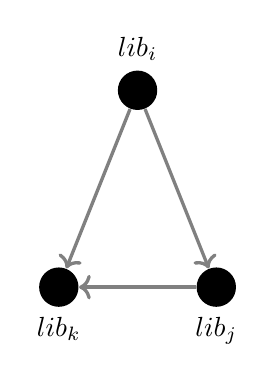
\begin{tikzpicture}[
         roundnode/.style={circle, fill=black, minimum size=5mm},
        squarenode/.style={fill=black, text=red, minimum size=5mm},
     ]
    \begin{scope}
         \node[roundnode, label=above:$lib_i$] (s2_proji) at (3, 2.5) {};
        \node[roundnode, label=below:$lib_j$] (s2_projj) at (4,0) {};
         \node[roundnode, label=below:$lib_k$] (s2_projk) at (2,0) {};
     \end{scope}

     \begin{scope} [every edge/.style={draw=gray, very thick}]
         \path [->] (s2_proji) edge (s2_projj);
         \path [->] (s2_proji) edge (s2_projk);
         \path [->] (s2_projj) edge (s2_projk);
     \end{scope}
     \end{tikzpicture}
    
     \caption{Example dependency graph for a given time period}
     \label{fig:lib}
     \vspace{2ex}
 \end{figure}
\begin{figure}[t]
    \centering

    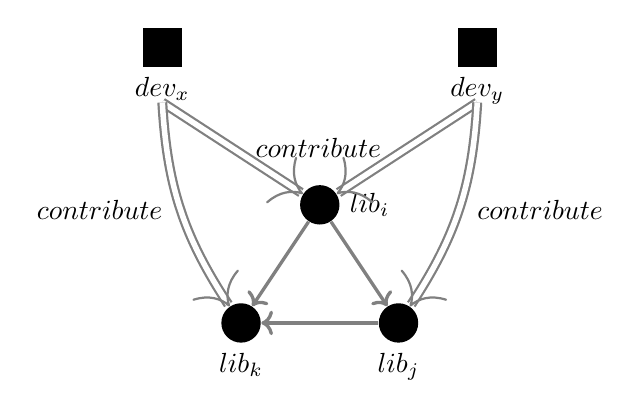
\begin{tikzpicture}[
        roundnode/.style={circle, fill=black, minimum size=5mm},
        squarenode/.style={fill=black, text=red, minimum size=5mm},
    ]
    \begin{scope}
        
        \node[roundnode, label=right:$lib_i$] (s2_proji) at (4, 1.5) {};
        \node[roundnode, label=below:$lib_j$] (s2_projj) at (5,0) {};
        \node[roundnode, label=below:$lib_k$] (s2_projk) at (3,0) {};
        
        \node[squarenode, label=below:$dev_x$] (s3_devx) at (2, 3.5) {};
        
        \node[squarenode, label=below:$dev_y$] (s3_devy) at (6, 3.5) {};
        
    \end{scope}

    \begin{scope} [every edge/.style={draw=gray, very thick}]
        \path [->] (s2_proji)  edge  (s2_projj);
        \path [->] (s2_proji) edge (s2_projk);
        \path [->] (s2_projj) edge (s2_projk);
        
    \end{scope}
    \begin{scope} [every edge/.style={draw=gray, thick, double distance=2pt}]
        \path [->] (6, 2.8) edge node[left = 2mm] {$contribute$} (s2_proji);
        \path [->] (6, 2.8) edge[bend left=15] node[right = 1mm] {$contribute$} (s2_projj);
        \path [->] (2, 2.8) edge node[right = 2mm] {$$} (s2_proji);
        \path [->] (2, 2.8) edge[bend right=15] node[left = 1mm] {$contribute$} (s2_projk);
    \end{scope}
    \end{tikzpicture}
\end{figure}
\begin{figure}[t]
    \centering
    \begin{tikzpicture}[
        roundnode/.style={circle, fill=black, minimum size=5mm},
        squarenode/.style={fill=black, text=red, minimum size=5mm},
    ]
    \end{tikzpicture}
\caption{Example Dependency-Contribution graph showing relationships between contributions and dependencies}
 \label{fig:dc-graph}
\end{figure}

This is just one example of the type of research that is enabled by access to heterogeneous data related to software package ecosystems.

\smallskip\noindent\textbf{Peril 1.}\textit{
 Developers might use different identifiers when contributing to different parts of a software package ecosystem, e.g., when contributing to different libraries.}\\
 
When modelling using such graphs, there is a threat that contributors may use multiple identifiers (i.e., $c_x$ and $c_y$ are the same contributor).
This is a well-known research problem, and there has been work to merge these accounts, such as \cite{wiese2016mailing}.
GitHub has introduced mechanisms such as two-factor authentication\footnote{\url{https://docs.github.com/en/authentication/securing-your-account-with-two-factor-authentication-2fa/configuring-two-factor-authentication}} to counteract the issue of multiple identifiers.
This is since developers might be less likely to switch accounts if it requires cumbersome authentication.


\smallskip\noindent\textbf{Peril 2.}\textit{
Developers' contributions to software package ecosystems might be interspersed with bot contributions, e.g., automated dependency updates.}\\

The rise of automation and artificial intelligence has led to much work on the integration of automated scheduling (i.e., bots) into software development workflows \cite{Storey2016, Farooq2016, Wessel2018, Erlenhov2019, bot_modify_wf} to name a few. These bots are designed to perform specific tasks within a software package ecosystem. For example, a bot may be programmed to automatically update dependencies, test code changes, or deploy software to production. As an example, the Google APIs repo-automation-bots project lists bots for automated labelling of issues and pull requests, automated approval of pull requests, and triggering releases.\footnote{\url{https://github.com/googleapis/repo-automation-bots}}
Bots perform common maintenance tasks in many software projects and are now commonplace \cite{Beschastnikh2017, Urli2018,BIMAN,bot_or_not}.
Especially with bots such as dependabot (automated pull requests to update configurations to reduce the risk of vulnerability threats),\footnote{\url{https://github.com/dependabot}} more and more automation has caused a lot of noise in the contributions between projects.
There are also bots for communication and documentation \cite{Urli2018, Lin2016, Lebeuf2017a}.

To be able to draw accurate conclusions about what humans are doing in software package ecosystems, researchers should consider distinguishing between bot and human contributions.
It is also important to differentiate this from other contributions \cite{maeprasart2022understanding}.
The research community has responded well, with a wide range of techniques and tools to mitigate this peril \cite{Bodegha2021, golzadeh2022accuracy}.

\smallskip\noindent\textbf{Peril 3.}\textit{
Not all developer activities in software package ecosystems are accessible to the public, e.g., library use in proprietary settings.
}\\

Not all developer activities in software package ecosystems are accessible to the public, e.g., when the boundary between open source and industry is blurred \cite{stol2014inner}, which presents a challenge for researchers who aim to study the development process. This is particularly true in proprietary settings where software development is performed behind closed doors or is open source for a limited time period, thus resulting in the artefacts not permanently being publicly available.
This can make it difficult to understand the broader ecosystem in which a software project is developed.
Proprietary settings may lead to non-standardisation in software development practises. Different software projects may use different management systems and tools, making it difficult to accurately compare and analyse software development activities across various projects. For example, some projects may use communication, documentation, and other management tools not captured on the same platform \cite{montgomery2022alternative}. For example, some projects might use Bugzilla instead of issues and pull requests for their bug and code review systems, while others may use Discord, Slack channels, or email threads for their communication needs.

This lack of standardisation in software development practises presents a challenge for researchers who study the software package ecosystem and understand the development process. To address this issue, researchers should strive to collect data from a diverse set of projects to gain a comprehensive understanding of the software package ecosystem. In addition, researchers may need to adjust their methodologies or data collection techniques to accommodate the different tools and practises used by different software projects.

\subsection{Defining Components and their Dependencies}

\smallskip\noindent\textbf{Promise 2.}\textit{
Researchers can access a software package ecosystem's dependency network through package managers and registries, e.g., npm lists the dependencies and dependents for over a million libraries.}\\


With the rise of curated datasets like libraries.io, researchers can now recover and model dependency relations between software units using pre-extracted datasets.
Table \ref{tab:PM_features} shows examples of popular package managers mined from the libraries.io dataset in 2020. 

\begin{table*}[]
\caption{Summary of 13 package managers from libraries.io as ranked by TIOBE in 2020}
 \label{tab:PM_features}
 \centering
\begin{tabular}{@{}llrlll@{}}
\toprule
\begin{tabular}[c]{@{}l@{}}Package \\ Ecosystem\end{tabular} & \begin{tabular}[c]{@{}l@{}}Programming \\ Language\end{tabular} &  \begin{tabular}[c]{@{}l@{}}Tiobe \\ Rank\end{tabular} & Environment & \begin{tabular}[c]{@{}l@{}}Dependency \\ Tree\end{tabular} & \begin{tabular}[c]{@{}l@{}}Package   \\Archive link\end{tabular}\\ \midrule
PyPI & Python & 2 & Python & Flat & pypi.org  \\
Maven & Java & 3 & JVM & Flat & Maven.org  \\
Bower & JavaScript & 7 & Node.js & Flat & bower.io  \\
Meteor & JavaScript & 7 & Node.js & Nested & atmospherejs.com \\
npm & JavaScript & 7 & Node.js & Nested (v2) & npmjs.com  \\
Packagist & PHP & 8 & PHP & Flat & packagist.org \\
Puppet & Ruby & 13 & Ruby MRI & Flat & forge.puppet.com  \\
RubyGems & Ruby & 13 & Ruby MRI & Flat & rubygems.org  \\
CRAN & R & 14 & RStudio & Flat & cran.r-project.org  \\
CPAN & Perl & 15 & Perl & Flat & metacpan.org  \\
GO & Golang & 20 & Go & Flat & pkg.go.dev  \\
NuGet & C\#, VB & 5, 6 & .NET & Flat & nuget.org \\
Anaconda & Python, R, C\# & 2, 14, 5 & Anaconda & Flat & anaconda.org  \\ \bottomrule
\end{tabular}
\end{table*}

\smallskip\noindent\textbf{Peril 4.}\textit{
Different software package ecosystems define the concept of ``dependency'' differently, e.g., by allowing or not allowing different versions of a library on the same dependency tree.
}\\

Different software package ecosystems have varying definitions of what constitutes a dependency. For example, some ecosystems may allow multiple versions of a library to exist on the same dependency tree, while others may restrict developers to a single version of a library \cite{Islam}. These restrictions are often based on the programming language being used, as different languages have different approaches to managing dependencies. It is important to consider the restrictions on dependency relationships when studying software package ecosystems, as they can have a major impact on the development process. For example, the ability to use multiple versions of a library on the same dependency tree can greatly simplify the process of updating dependencies and can make it easier to resolve conflicts between libraries.

One way to visualise the impact of these restrictions is to compare the difference between a nested dependency tree and a directed dependency tree, as shown in Figure \ref{fig:nest}.\footnote{Taken from \url{https://npm.github.io/how-npm-works-docs/npm3/how-npm3-works.html}} This distinction is important because it highlights the different ways that a software unit can depend on different versions of the same library.
In this example, npm v3 creates the dependency tree based on the installation order, therefore flattening unnecessary nested dependencies (i.e., B v1.0 in cyan). This reduces the complexity of a nested tree by resolving some of the transitive dependencies (nested dependencies).

\begin{figure}
	\centering
	\includegraphics[width=.8\textwidth]{book/chapter-promisesandperils/pics/nestedv2.jpg}
	\caption{Difference between flat and nested dependencies}
	\label{fig:nest}
\end{figure}

\smallskip\noindent\textbf{Peril 5.}\textit{
Developers might declare a dependency to other parts of a software package ecosystem but not use it, e.g., because they failed to update its removal.
}\\

It is common for developers to declare dependencies on other parts of the software package ecosystem but not always use them. This can happen for various reasons, such as forgetting to remove the dependency after it is no longer needed. This can pose a challenge for researchers who are trying to extract dependencies from package managers, like those in configuration files, as there may be inconsistencies between the listed dependencies and what is actually being compiled and used by the code. This can lead to a biased understanding of the software package ecosystem and the relationships between software components.

To address this issue, there have been numerous efforts to track the actual library dependencies compiled and executed in software systems. These efforts aim to provide a more accurate understanding of the dependencies and the relationships between software components. For example, research has been conducted on the use of dynamic analysis to track compiled dependencies in real time and on the development of tools to automatically detect and track executed dependencies \cite{Zapata:ICSME2018, Ponta2018,Chinthanet:ASE2020}.

\subsection{Defining Boundaries and Completeness}

\smallskip\noindent\textbf{Promise 3.}\textit{
Researchers can use the boundaries of software package ecosystems to study communities of developers, e.g., developers contributing to and/or benefiting from the npm ecosystem.
}\\

Following Promise 2, the emergence of package managers has also led to studies that approximate software communities.
Using the libraries.io dataset, researchers were able to study projects that host libraries that use package managers.
Researchers have used this dataset to compare different library ecosystems \cite{kikas.2017,decan:emse:2019,CogoDown2019}.


\smallskip\noindent\textbf{Peril 6.}\textit{
Package managers do not always represent software package ecosystems, their communities, or their sub-communities, e.g., in cases where multiple package managers exist.
}\\

Package managers are a fundamental aspect of software package ecosystems, but do not always fully represent the complex relationships and interactions that occur within a community of developers and users, as shown in Table~\ref{tab:PM_features}. In some cases, multiple package managers exist for the same programming language, creating a complex landscape of software libraries and dependencies that are not always easily understood. For instance, Bower and Meteor manage npm libraries, which can lead to confusion and overlap in the management of dependencies.

Similarly, Java, Scala, Android, and other Java-based open source communities all use the Maven package manager, but each of these communities has its own unique set of libraries, dependencies, and development practises. Researchers should be aware of the limitations of package managers when studying software package ecosystems, and consider the broader context and relationships that exist within these communities. 

\smallskip\noindent\textbf{Peril 7.}\textit{
Lack of activity in parts of a software package ecosystem does not necessarily indicate project failure, e.g., when highly depended-upon libraries are feature-complete.
}\\

It is important to note that lack of activity in a part of a software package ecosystem does not always mean project failure \cite{coelho2017modern}. In some cases, highly relied-upon libraries that have reached feature-completeness may see little activity, but continue to be used by the software community. 

However, it is still important to consider the long-term sustainability of these libraries, especially given the rate at which technology and software development practises change. This has become a topic of interest in recent years, and researchers have explored best practises for sustaining open source projects and ensuring their continued success \cite{Ait2022,valiev2018ecosystem}. Understanding the factors that contribute to project sustainability is important to ensure the longevity and continued growth of software package ecosystems.

\smallskip\noindent\textbf{Peril 8.}\textit{
Sampling from a software package ecosystem is challenging since sub-setting might alter the dependency network, e.g., by breaking dependency chains.
}\\

Sampling from a package ecosystem is not straightforward, as the sample composition can be significantly affected due to missing dependency links between libraries. For instance, a subset of the ecosystem might alter the dependencies between libraries, leading to the breakdown of the dependency chains. This could lead to an incomplete picture of the software package ecosystem, leading to incorrect conclusions from a study. To minimise this risk, researchers should carefully consider the boundaries of their study and choose the appropriate sampling method based on the research questions and goals. For example, researchers could focus on popular, highly dependent, or risk-vulnerable aspects of the ecosystem as a starting point. 
For some ecosystems, the number of downloads, GitHub stars, and watchers are other aspects for the researcher to utilise.


\smallskip\noindent\textbf{Peril 9.}\textit{
Sampling from a software package ecosystem is challenging since the dependency network changes over time, e.g., when dependencies are added, removed, upgraded, or downgraded.
}\\

The dynamic nature of package ecosystems and the constant changes to their dependencies can impact the generalisability of the results. Therefore, it is important to also consider the time granularity of the analysis. For example, if the goal is to understand the evolution of dependencies over time, a finer time granularity may be necessary to capture the smaller changes and trends. However, if the goal is to understand the overall structure and relationships within the ecosystem, a coarser time granularity may be sufficient. Based on recent studies \cite{wattanakriengkrai2022giving,valiev2018ecosystem,Mirsaeedi:icse2020, Brindescu:emse2020, Nassif:icsme2017}, a three-month window seems appropriate for some studies.
Another level of granularity to consider is the size of the component. For instance, there are cases where a single package may contain more than one repository, especially for large library frameworks. 
The granularity also depends on the nature of the ecosystem itself. For instance, researchers should understand whether the ecosystem comprises library packages (e.g., PyPI), plugins (e.g., Eclipse), or is a library distribution (e.g., Android).



\subsection{Analysing and Visualising the Data}

\textbf{Peril 10.}\textit{
Analysing and visualising entire software package ecosystems is challenging due to their size, e.g., in terms of nodes and edges in the network.
}\\

The size of software package ecosystems implies large data sets, which can be overwhelming for tools and algorithms to analyse and display. Therefore, it may be necessary to make choices about the granularity of the data included in the analysis and visualisation. Another alternative is to focus on the most critical parts of the software package ecosystem, such as the high-level structure, highly dependent packages, or parts of the system that pose a risk to security and reliability. 
The key is to strike a balance between detail and simplicity, providing a meaningful representation of the ecosystem while being able to handle the complexity of its size.


\section{Application: When to Apply Which Peril}
\label{PPM:sec:application}

We include a disclaimer stating that not all perils are applicable to every mining situation. To demonstrate the practical application of our perils and their mitigation, we present two case studies that involve mining the software package ecosystem. Each case study has a distinct research objective and focusses on a specific dataset to be mined.

\subsection{Two Case Studies}
Table \ref{tab:cases} presents the two case studies we have selected for this analysis.
The \textit{first case} involves mining for contributions congruent to dependency updates \cite{wattanakriengkrai2022giving}. 
In this work, the authors mine GitHub repositories for Pull Requests and Issues that were submitted and merged congruent to dependency updates within the npm ecosystem. 
The \textit{second case} involves mining communication data for the Eclipse ecosystem \cite{Nugroho2021}. Although the second case does not mine for dependency relations (i.e., use relations),  we show that these perils still apply when mining for other relationships in an ecosystem.
Moreover, the second case studies the Eclipse ecosystem, which is a different dataset compared to the more popular GitHub dataset.

\subsection{Applying Perils and their Mitigation Strategies}
Table \ref{tab:perilsapp} provides a summary of the perils that can be applied to each of the case studies. We will now go into the details of mitigation strategies based on these perils. 
For better organisation and understanding, we have grouped the perils according to the four logical processes for mining.

\smallskip\noindent\textbf{Information to Mine}. 
The first set of mitigation strategies, which addresses perils 1-3, focusses on planning which information to mine. There are two primary strategies that researchers can employ:


\begin{enumerate}
    \item Researchers should use research tools and techniques to remove noise and other biases in the dataset, such as bot detection and the handling of multiple identities. This strategy was implemented in both case studies, as contributions and discussions often have the potential to involve bots or developers with multiple identities.
\item Depending on the research goals, researchers should recognise that not all contributions are equal and filter the dataset accordingly.
\end{enumerate}

We applied these two strategies to both cases. In the first case, the goal was to capture all congruent contributions, so we filtered out contributions made to libraries without dependencies. Since all npm packages are listed in the registry, Peril 3 (private activities) did not apply.
In the second case, we addressed Peril 1 by conducting a qualitative analysis to ensure that the member identities were not duplicated, as Eclipse developers were known to change identities. To mitigate Peril 2, we removed bot responses. For the second case, since all forum data is made public, Peril 3 did not apply.


\begin{table}
\centering
\caption{Description of the research objectives and datasets for the case studies}
 \label{tab:cases}
\begin{tabular}{lp{5cm}r} 
\toprule
\textbf{Case Study} & \textbf{Research Objective}                                                          & \textbf{Datasets}           \\
\midrule
Wattanakriengkrai \etal \cite{wattanakriengkrai2022giving}             & Explore code contributions between library and client (i.e, use-relations)  & libraries.io\\
& &  GitHub API \\
Nugroho \etal \cite{Nugroho2021}                & Explore discussion contributions between contributors (i.e., contributions) & Eclipse API                \\
\bottomrule
\end{tabular}
\end{table}

\begin{table}
\centering
\caption{Application of each peril to the case studies}
 \label{tab:perilsapp}
\begin{tabular}{rp{8cm}ccc} 
\toprule                   
& \textbf{Perils}       & case 1      & case 2                 \\
                                                                               & & npm  & Eclipse   \\
\midrule
\textbf{P1} &Developers might use different identifiers when contributing to different parts of a software package ecosystem, e.g., when contributing to different libraries.                             &    \CheckedBox         &          \CheckedBox           \\ 
%\hline
\textbf{P2} & Developers' contributions to software package ecosystems might be interspersed with bot contributions, e.g., automated dependency updates.                                                      &      \CheckedBox               &      \CheckedBox               \\ 
%\hline
\textbf{P3} & Not all developer activities in software package ecosystems are accessible to the public, e.g., library use in proprietary settings.                                                         &         -           &      \CheckedBox               \\ 
%\hline
\textbf{P4} & Different software package ecosystems define the concept of \`{}\`{}dependency'' differently, e.g., by allowing or not allowing different versions of a library on the same dependency tree. &         \CheckedBox       &     -                            \\ 
%\hline
\textbf{P5} & Developers might declare a dependency to other parts of a software package ecosystem but not use it, e.g., because they failed to update its removal.                                        &     -           &  -    \\
%\hline
\textbf{P6} &Package managers do not always represent software package ecosystems, their communities, or their sub-communities, e.g., in cases where multiple package managers exist.                     &     -                   &  -                  \\
%\hline
\textbf{P7} & Lack of activity in parts of a software package ecosystem does not necessarily indicate project failure, e.g., when highly depended-upon libraries are feature-complete.                     &       \CheckedBox         &  -                           \\
%\hline
\textbf{P8} &Sampling from a software package ecosystem is challenging since sub-setting might alter the dependency network, e.g., by breaking dependency chains.                                         &        \CheckedBox        &     \CheckedBox                                \\
%\hline
\textbf{P9} &Sampling from a software package ecosystem is challenging since the dependency network changes over time, e.g., when dependencies are added, removed, upgraded, or downgraded.               &       \CheckedBox         &     -                          \\
%\hline
\textbf{P10} &Analysing and visualising entire software package ecosystems is challenging due to their size, e.g., in terms of nodes and edges in the network.                                  &        \CheckedBox      &      \CheckedBox               \\
\bottomrule
\end{tabular}
\end{table}

\smallskip\noindent\textbf{Defining Dependencies}. 
The second set of perils (Perils 4-5) is related to dependency relationships between software units, and only the first case study is applicable. To address these perils, researchers should adopt the following strategy:

\begin{enumerate}
    \item Researchers should not rely solely on listed dependencies in configuration files (e.g., pom.xml, package.json, etc.) as a measure of dependency between two components. Instead, code-centric approaches should be used to validate which libraries are actually depended upon.
\end{enumerate}

For example, in the first case, in addition to mining the configuration information, the authors also analysed the similarity of the source code contributions to address Peril 4. Regarding Peril 5, since the study's objective was to investigate changes to the configuration files, the risk of the update not being executed was deemed less important.
It is important to note that the second case study did not include dependency analysis and, therefore, these perils did not apply.

\begin{figure*}[]
    \centering
    \begin{subfigure}{0.9\linewidth}
         \includegraphics[width=1.1\textwidth]{book/chapter-promisesandperils/pics/congruentViz.jpg}
         \caption{Visualization of a Time analysis for 107,242 libraries.}
     \end{subfigure}
     \begin{subfigure}{0.9\linewidth}
         \includegraphics[width=1\textwidth]{book/chapter-promisesandperils/pics/eclipseViz.jpg}
         \caption{A Visual Topology map for 832,058 threads}
     \end{subfigure}
    \caption{Visualisation examples for the two case studies}
    \label{fig:visCase}
\end{figure*}

\smallskip\noindent\textbf{Defining Boundaries}.
The third set of perils (Perils 6-9) is related to the definition of boundaries and completeness and is relevant for both case studies. To mitigate these perils, we recommend the following strategies:

\begin{enumerate}
    \item Researchers should recognise that a dormant project does not necessarily mean that it is inactive. Instead, studies can use alternative heuristics, such as the number of dependents and dependencies, as better indicators of a project's importance in the ecosystem.
    \item Researchers should not rely solely on the programming language to define sub-communities. Using a common package manager for the programming language is a more effective rule of thumb for distinguishing boundaries.
    \item Researchers should avoid random sampling. Instead, sampling should be tailored to the research goals by considering factors such as an appropriate time window or focussing on specific attributes of components (e.g., most dependents, most popular, most contributors).
\end{enumerate}


Peril 6 did not apply to any of the case studies. 
Particularly for the first case, since the goal was to explore the npm package ecosystem, we assumed that the boundaries were clearly defined by the npm registry. 
Similarly, the second case study used the generic Eclipse platform as the boundary. 
Peril 7 was applied to the npm study, while Peril 8 was applied to both case studies. 
As a result, the two cases conducted a qualitative analysis of the dataset to gain deeper insights.
In the first case study, a three-month time window was created to capture dependencies. 
For the second case study, forum contributors were sampled into three groups (i.e., junior, member, or senior) according to the sliding window of their contributions. 

\smallskip\noindent\textbf{Visualisation}.
The final peril (Peril 10) relates to visualisation, which can be challenging due to the vast size and complexity of software ecosystems. As it is not feasible to visualise every aspect of an ecosystem simultaneously, a focused approach is necessary. A mitigation strategy is to select specific attributes of the ecosystem (e.g., the most dependent, most popular, and most contributions) that align with the research needs and objectives. 

Figure \ref{fig:visCase} shows two cases where visualizations are employed to gain insights, especially for large datasets.
In the first figure (a), we visualize the distributions of the data set and applied the appropriate statistical tests, along with the effect size, to test our hypotheses and answer research questions. 
In the second example (b), although not directly related to package ecosystems, the authors utilized a topological visualization \cite{Lum2013ExtractingIF} to gain insights on the over 800,000 forum threads of discussions. 



\section{Chapter Summary}
In this chapter, we explore the various aspects of mining information from the software package ecosystem, presenting three promises and ten perils that researchers should be aware of when undertaking such tasks. The chapter is structured around four key processes for mining: 1) Planning what Information to Mine, 2) Defining Components and their Dependencies, 3) Defining Boundaries and Completeness, and 4) Analysing and Visualising the Data. To help new and experienced researchers navigate these challenges, we introduced the SUG model, which can serve as a valuable tool to minimise threats to validity. Although some perils may be more relevant to specific research objectives, our aim is to equip researchers with the knowledge and resources needed to confidently gather and integrate software package ecosystem data into their work.
%Workflow automation in software development ecosystems (working title)
% %Semantic labeling three-letter-code: WFA (e.g. \chapter{WFA})

% 
\title{Promises and Perils of Mining \\ Software Package Ecosystem Data}
\author{Raula Gaikovina Kula \and Katsuro Inoue \and Christoph Treude}
\institute{Raula Gaikovina Kula \at Nara Institute of Science and Technology, Japan, \email{raula-k@naist.jp}
\and Katsuro Inoue \at Nanzan University, Japan \email{ inoue599@nanzan-u.ac.jp}
\and  Christoph Treude \at The University of Melbourne, Australia \email{christoph.treude@unimelb.edu.au}}

\maketitle
\label{PPM:ch}
\abstract*{The use of third-party packages is becoming increasingly popular and has led to the emergence of large software package ecosystems with a maze of inter-dependencies. Since the reliance on these ecosystems enables developers to reduce development effort and increase productivity, it has attracted the interest of researchers: understanding the infrastructure and dynamics of package ecosystems has given rise to approaches for better code reuse, automated updates, and the avoidance of vulnerabilities, to name a few examples. But the reality of these ecosystems also poses challenges to software engineering researchers, such as: How do we obtain the complete network of dependencies along with the corresponding versioning information? What are the boundaries of these package ecosystem? How do we consistently detect dependencies that are declared but not used? How do we consistently identify developers within a package ecosystem? How much of the ecosystem do we need to understand to analyse a single component? How well do our approaches generalise across different programming languages and package ecosystems? In this chapter, we review promises and perils of mining the rich data related to software package ecosystems available to software engineering researchers.}

\abstract{The use of third-party packages is becoming increasingly popular and has led to the emergence of large software package ecosystems with a maze of inter-dependencies. Since the reliance on these ecosystems enables developers to reduce development effort and increase productivity, it has attracted the interest of researchers: understanding the infrastructure and dynamics of package ecosystems has given rise to approaches for better code reuse, automated updates, and the avoidance of vulnerabilities, to name a few examples. But the reality of these ecosystems also poses challenges to software engineering researchers, such as: How do we obtain the complete network of dependencies along with the corresponding versioning information? What are the boundaries of these package ecosystems? How do we consistently detect dependencies that are declared but not used? How do we consistently identify developers within a package ecosystem? How much of the ecosystem do we need to understand to analyse a single component? How well do our approaches generalise across different programming languages and package ecosystems? In this chapter, we review promises and perils of mining the rich data related to software package ecosystems available to software engineering researchers.}

%%%%%%%%%%%%%%%%%%%%%%%%%%%%%%%%%%%%%%%%%%%%%%%%%%%%%%%%%%%%%%%%%%

\section{Introduction}
\label{PPM:sec:definition}

Third-party libraries are a great way for developers to incorporate code without having to write their own for every functionality required. By using these libraries, developers can save time and energy while still getting the functions they need.
Using third-party libraries is becoming increasingly popular and has led to the emergence of large software package ecosystems such as npm. While these ecosystems offer many benefits, they also come with risks, such as software vulnerability attacks \cite{Chinthanet:ASE2020}.

Large software package ecosystems are a treasure trove for researchers who can investigate a wide range of questions. For example, by studying activity in large ecosystems, researchers can identify which libraries are the most popular and learn what characteristics make them successful \cite{kikas.2017,decan:emse:2019}.
Additionally, research on large ecosystems can help developers understand how to protect their code from malicious actors who may attempt to exploit vulnerabilities or insert malware into popular libraries.
Studying large software package ecosystems can help us better understand the dynamics of open source development in general. Open source development is a complex process that involves many different stakeholders working together (or sometimes competing) to create valuable code that anyone can use or improve upon. By understanding how these interactions play out in different types of ecosystem structures -- including those with many small projects versus few very large ones -- we can develop insights that might be applicable more broadly across other types of collaborative systems.

In this chapter, we identify and discuss promises and perils during the mining process, ranging from planning what information to mine from the ecosystem to analysing and visualising the mined data. 
Therefore, the chapter is broken down into these logical processes of mining ecosystem data: 1) Planning what Information to Mine, 2) Defining Components and their Dependencies, 3) Defining Boundaries and Completeness, and 4) Analysing and Visualising the Data.

This chapter is intended for researchers and practitioners who are interested in exploring and exploiting software package ecosystem information from a diverse range of sources that are publicly available. 
We also highlight the pitfalls to consider during the mining process, particularly when these pitfalls could lead to a misinterpretation of the analysis and results. 
The chapter is written in a manner that encourages newcomers who have little or no experience or who are interested in utilising ecosystem data across different disciplines outside of software engineering.
Our goal is to get new researchers quickly accustomed to gathering ecosystem information for their research.


\section{A Component-based Software Ecosystem}

Defined as a component-based software ecosystem, we suggest using the term `software package ecosystem' as a suitable term for the symbiotic relationships among third-party library components (as software projects or repositories), as these libraries and their dependent clients coexist on the same technological platform, therefore sharing the same environment and other internal and external factors (e.g., security threats, sharing contributions, etc.).
Please refer to the Introduction chapter for an in-depth definition of the different types of software ecosystems.
We present our interpretation of the software package ecosystem in Kula et al.~\cite{KulaSANER18}, where we formally define a package ecosystem using a Software Universe Graph (SUG).
This is modelled as a structured abstraction of the evolution of software systems and their library dependencies over time.

%%%%%%%%%%%%%%%%%%%%%%%%%%%%%%%%%%%%%%%%%%
\begin{figure*}
	\centering
	\includegraphics[width=.7\textwidth]{book/chapter-promisesandperils/pics/UniversalExample.jpg}
	\caption{Conceptual example of the Software Universe Graph, depicting the use and update relationships between different software units.}
	\label{fig:SUG}
\end{figure*}
%%%%%%%%%%%%%%%%%%%%%%%%%%%%%%%%%%%%%%%%%%%%%


\paragraph{\textbf{Component-based Representation as a Software Universe Graph}}
\label{PPM:sec:SUG}

First introduced by Kula et al.~\cite{KulaSANER18}, the \textit{Software Universe Graph} (SUG) is a structural abstraction of the software ecosystem of third-party libraries.
Figure \ref{fig:SUG} provides an illustration of the different relationships within the graph.
Let $G= (N,E)$ represent a graph $G$. $N$ is a set of nodes, each node representing a software unit. 
We define a software unit as a version instance of any software program. 

The authors then present the \textit{use} and \textit{update} relationships that exist in the ecosystem.
Hence, the edges $E$ are composed of $E_{use}$ and $E_{update}$. $E_{use}$ is a set of \textit{use-relations} and $E_{update}$ is a set of \textit{update-relations}.

\begin{definition}
An edge $u \rightarrow v \in E_{use}$ means that $u$ uses $v$. The defined functions of $E_{use}$ are:

\begin{equation}
\small
\small \use(u)\equiv \{v|u \rightarrow v\}
\normalsize
\end{equation}
\begin{equation}
\small
\small \useBy(u)\equiv \{v|v \rightarrow u\}
\normalsize
\end{equation}
\end{definition}

Use-relations can be extracted from either the source code or configuration files. 
As shown in Figure \ref{fig:SUG}, node $a1$ uses node $x1$. 
In addition, node $x1$ is used by nodes $a1$, $q1$, and $q2$. Parallel edges for node pairs are not allowed.

\begin{definition}
We represent an update relation from node $a$ to $b$ using $ a \Rightarrow b $, which means that the newer update $b$ was released from node $a$ and is defined as:
\begin{equation}
\small a \Rightarrow b \in E_{update}
\end{equation}
\end{definition}

Update relations refer to when a successive release of a software unit is made available. Figure \ref{fig:SUG} shows that node $q1$ is first updated to node $q2$. Later, node $q2$ is updated to the latest node $q3$. Hence, $q1 \Rightarrow q2 \Rightarrow q3$.
Note that an update should not be confused with forking. 
We distinguish a fork as a separate software unit. 
Each node in the SUG should be denoted by three attributes: \texttt{<name,release,time>}.  
For a node $u$, we define:

\begin{itemize}
	\item \textbf{u.name} Name is the string representation identifier of a software unit.
	We introduce the name axiom: For nodes $u$ and $v$, if $u \Rightarrow v$, then $u.name = v.name$ holds.
	
	\item \textbf{u.release}. Release refers to the specific assigned change reference for a software unit. For nodes $u$ and $v$, if $u \Rightarrow v$
	then $v$ is the immediate successor of $u$. Note that the versioning pattern may vary from project to project. 
	\item \textbf{u.time}. Time refers to the time stamp at which node $u$ was released. For nodes $u$ and $v$ of $u \Rightarrow v$, $u.time < v.time$.
\end{itemize}

\begin{figure}
	\centering
	\includegraphics[width=.8\textwidth]{book/chapter-promisesandperils/pics/TemporalSUG.jpg}
	\caption{Temporal property of the SUG}
	\label{fig:SUGTemp}
\end{figure}

\begin{definition}
    
	The SUG has temporal properties.
This describes the simultaneity or ordering in reference to time. Let SUG $G = (N, E) $ be at time $t$. At time $t^{\prime} > t$, we observe an extension of $G$, such that:

\begin{equation}
\small G^{\prime} = (N \cup \Delta N, E \cup \Delta E)
\end{equation}
where $\Delta E \cap (N \times N) = \emptyset$
\end{definition}

Figure \ref{fig:SUGTemp} illustrates the temporal properties of the SUG. 
Here, it is observed that $G'$ is composed of $G$ augmented with newly added node $a3$ and its corresponding $a3 \rightarrow x2$ and $a2 \Rightarrow a3$ relations.
A SUG grows monotonically over time with only additions.
Here, we consider that modification or deletion changes on the SUG do not occur. 

\begin{definition}
    A timed SUG specifies the state of the SUG at any point in time.
So for an SUG $G=(N,E)$, we represent a timed SUG $G_{t}$ at time $t$ as a sub-graph of $G$. Formally,
\begin{equation}
\small G_t\equiv(N_{t}, E_{t})
\end{equation}
where $N_{t} = \{u|u \in N, u.time \leq t \}$ and $E_t = \{ e | e \in E \wedge e \in  N_t \}$
\end{definition}
	


\section{Data Sources}
Researchers can use various datasets to model the ecosystem using the SUG model of usage and update relationships.
The most obvious data source that has revolutionised data mining in the software engineering domain is the GitHub platform. 
Established in 2008, and then purchased by Microsoft in 2020, GitHub is home to various popular Open Source Software. 
GitHub is built on the git version control system and is useful for storing all changes made to a repository. 
In the case of the SUG, a GitHub repository can represent one software unit, whose depend relations can be extracted via a configuration file (such as the package.json file for JavaScript projects).
The repository should also contain the release information that holds the update relations.
Due to its large size, researchers and the GitHub team have made available datasets for researchers to mine, for example through the GitHub API/Graph QL.\footnote{\url{https://docs.github.com/en/graphql}} This is the backend Application Programming Interface (API) that can be used to query large amounts of data on GitHub. Most researchers use the API to download and mine information from the GitHub platform. 
It is important to note that while GitHub introduced a new feature of Dependency Graphs to map the depend relationship,\footnote{\url{https://docs.github.com/en/code-security/supply-chain-security/understanding-your-software-supply-chain/about-the-dependency-graph}} most older projects do not have this feature.
In this case, the researcher would need to manually extract and query the configuration files for dependency information. 

We refer to the first chapter for additional information on data sources for mining software ecosystems. 

\section{Promises and Perils}
\label{PPM:sec:promisesperils}

Using the SUG model of depend and use relations and the available datasets, we can now present our promises and perils of mining ecosystem information.

\subsection{Planning What Information to Mine}

\textbf{Promise 1.}\textit{
Researchers can access and link heterogeneous data related to software package ecosystems, e.g., package registries and bug trackers.}\\

When planning what information to mine from the ecosystem, researchers do not need to limit themselves to the usage and update relationship information.
Platforms that host software repositories include other software management systems such as bug trackers.
For example, GitHub allows researchers to manage GitHub Pull Requests, Issues, and Discussions not only for one project, but for multiple projects.
GitHub provides three management systems that are related to a software repository:

\begin{itemize}
    \item \textit{GitHub Discussions}\footnote{\url{https://docs.github.com/en/discussions}} - The GitHub Discussions forum is a collaborative communication forum for the community around an open source or internal project. Community members can ask and answer questions, share updates, have open-ended conversations, and follow along on decisions affecting the community's way of working.
    \item \textit{GitHub Pull Requests}\footnote{\url{https://docs.github.com/en/pull-requests}} - Pull Requests allow other developers from an ecosystem to make a contribution to a software repository. Pull requests also allow maintainers to discuss and review potential changes with collaborators and add follow-up commits before changes are merged into the software.
    \item \textit{GitHub Issues}\footnote{\url{https://docs.github.com/en/issues}} - Issues are used to track ideas, feedback, tasks, or bugs for work on GitHub.
\end{itemize}

These three systems are examples of how developers contribute to both their own and other projects. 
Hence, to incorporate this information, we can extend the SUG model, creating a model that includes a contribution relationship \cite{wattanakriengkrai2022giving}.

% Note that other platforms may also have management systems, like GitLab, BitBucket and Eclipse.

\begin{definition}
	A Dependency-Contribution graph incorporates contributions by developers whose libraries are involved in dependency relationships. 
\end{definition}

In this work \cite{wattanakriengkrai2022giving}, the authors explore the congruence between dependency updates and developer contributions, based on the original concept of social-technical congruence \cite{stcCataldo2008} where developers contribution patterns are congruent with their coordination needs. Hence, the goal is to identify contributions that are congruent to dependency updates.
As shown in Figure \ref{fig:lib} the authors extend from the typical SUG graph model where $lib_i$ depends (use) on  $lib_k$ and  $lib_j$, while  $lib_j$ also depends on $lib_k$, to the example shown in Figure \ref{fig:dc-graph}.
Different to the SUG, the graph captures developers and their contributions (i.e., the square as $dev_x$ and $dev_y$ represent two different developers making a contribution).
Here contributions are defined as $c$ (Pull Request or Issue) that were submitted to both a library and the client that depends on that library.
Hence, the graph can show contributions that are congruent to dependency changes for a software unit. 

\begin{figure}[t]
     \centering
     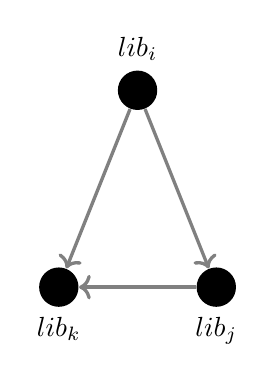
\begin{tikzpicture}[
         roundnode/.style={circle, fill=black, minimum size=5mm},
        squarenode/.style={fill=black, text=red, minimum size=5mm},
     ]
    \begin{scope}
         \node[roundnode, label=above:$lib_i$] (s2_proji) at (3, 2.5) {};
        \node[roundnode, label=below:$lib_j$] (s2_projj) at (4,0) {};
         \node[roundnode, label=below:$lib_k$] (s2_projk) at (2,0) {};
     \end{scope}

     \begin{scope} [every edge/.style={draw=gray, very thick}]
         \path [->] (s2_proji) edge (s2_projj);
         \path [->] (s2_proji) edge (s2_projk);
         \path [->] (s2_projj) edge (s2_projk);
     \end{scope}
     \end{tikzpicture}
    
     \caption{Example dependency graph for a given time period}
     \label{fig:lib}
     \vspace{2ex}
 \end{figure}
\begin{figure}[t]
    \centering

    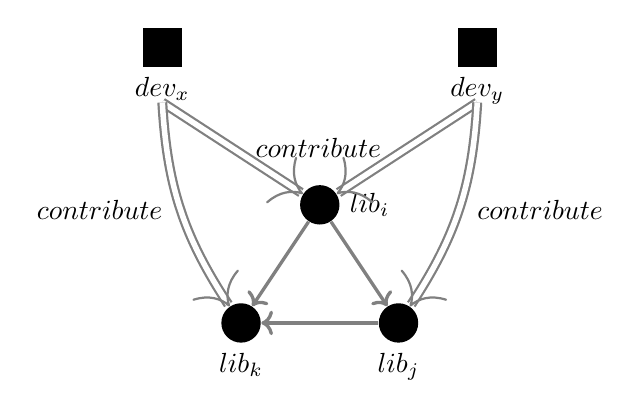
\begin{tikzpicture}[
        roundnode/.style={circle, fill=black, minimum size=5mm},
        squarenode/.style={fill=black, text=red, minimum size=5mm},
    ]
    \begin{scope}
        
        \node[roundnode, label=right:$lib_i$] (s2_proji) at (4, 1.5) {};
        \node[roundnode, label=below:$lib_j$] (s2_projj) at (5,0) {};
        \node[roundnode, label=below:$lib_k$] (s2_projk) at (3,0) {};
        
        \node[squarenode, label=below:$dev_x$] (s3_devx) at (2, 3.5) {};
        
        \node[squarenode, label=below:$dev_y$] (s3_devy) at (6, 3.5) {};
        
    \end{scope}

    \begin{scope} [every edge/.style={draw=gray, very thick}]
        \path [->] (s2_proji)  edge  (s2_projj);
        \path [->] (s2_proji) edge (s2_projk);
        \path [->] (s2_projj) edge (s2_projk);
        
    \end{scope}
    \begin{scope} [every edge/.style={draw=gray, thick, double distance=2pt}]
        \path [->] (6, 2.8) edge node[left = 2mm] {$contribute$} (s2_proji);
        \path [->] (6, 2.8) edge[bend left=15] node[right = 1mm] {$contribute$} (s2_projj);
        \path [->] (2, 2.8) edge node[right = 2mm] {$$} (s2_proji);
        \path [->] (2, 2.8) edge[bend right=15] node[left = 1mm] {$contribute$} (s2_projk);
    \end{scope}
    \end{tikzpicture}
\end{figure}
\begin{figure}[t]
    \centering
    \begin{tikzpicture}[
        roundnode/.style={circle, fill=black, minimum size=5mm},
        squarenode/.style={fill=black, text=red, minimum size=5mm},
    ]
    \end{tikzpicture}
\caption{Example Dependency-Contribution graph showing relationships between contributions and dependencies}
 \label{fig:dc-graph}
\end{figure}

This is just one example of the type of research that is enabled by access to heterogeneous data related to software package ecosystems.

\smallskip\noindent\textbf{Peril 1.}\textit{
 Developers might use different identifiers when contributing to different parts of a software package ecosystem, e.g., when contributing to different libraries.}\\
 
When modelling using such graphs, there is a threat that contributors may use multiple identifiers (i.e., $c_x$ and $c_y$ are the same contributor).
This is a well-known research problem, and there has been work to merge these accounts, such as \cite{wiese2016mailing}.
GitHub has introduced mechanisms such as two-factor authentication\footnote{\url{https://docs.github.com/en/authentication/securing-your-account-with-two-factor-authentication-2fa/configuring-two-factor-authentication}} to counteract the issue of multiple identifiers.
This is since developers might be less likely to switch accounts if it requires cumbersome authentication.


\smallskip\noindent\textbf{Peril 2.}\textit{
Developers' contributions to software package ecosystems might be interspersed with bot contributions, e.g., automated dependency updates.}\\

The rise of automation and artificial intelligence has led to much work on the integration of automated scheduling (i.e., bots) into software development workflows \cite{Storey2016, Farooq2016, Wessel2018, Erlenhov2019, bot_modify_wf} to name a few. These bots are designed to perform specific tasks within a software package ecosystem. For example, a bot may be programmed to automatically update dependencies, test code changes, or deploy software to production. As an example, the Google APIs repo-automation-bots project lists bots for automated labelling of issues and pull requests, automated approval of pull requests, and triggering releases.\footnote{\url{https://github.com/googleapis/repo-automation-bots}}
Bots perform common maintenance tasks in many software projects and are now commonplace \cite{Beschastnikh2017, Urli2018,BIMAN,bot_or_not}.
Especially with bots such as dependabot (automated pull requests to update configurations to reduce the risk of vulnerability threats),\footnote{\url{https://github.com/dependabot}} more and more automation has caused a lot of noise in the contributions between projects.
There are also bots for communication and documentation \cite{Urli2018, Lin2016, Lebeuf2017a}.

To be able to draw accurate conclusions about what humans are doing in software package ecosystems, researchers should consider distinguishing between bot and human contributions.
It is also important to differentiate this from other contributions \cite{maeprasart2022understanding}.
The research community has responded well, with a wide range of techniques and tools to mitigate this peril \cite{Bodegha2021, golzadeh2022accuracy}.

\smallskip\noindent\textbf{Peril 3.}\textit{
Not all developer activities in software package ecosystems are accessible to the public, e.g., library use in proprietary settings.
}\\

Not all developer activities in software package ecosystems are accessible to the public, e.g., when the boundary between open source and industry is blurred \cite{stol2014inner}, which presents a challenge for researchers who aim to study the development process. This is particularly true in proprietary settings where software development is performed behind closed doors or is open source for a limited time period, thus resulting in the artefacts not permanently being publicly available.
This can make it difficult to understand the broader ecosystem in which a software project is developed.
Proprietary settings may lead to non-standardisation in software development practises. Different software projects may use different management systems and tools, making it difficult to accurately compare and analyse software development activities across various projects. For example, some projects may use communication, documentation, and other management tools not captured on the same platform \cite{montgomery2022alternative}. For example, some projects might use Bugzilla instead of issues and pull requests for their bug and code review systems, while others may use Discord, Slack channels, or email threads for their communication needs.

This lack of standardisation in software development practises presents a challenge for researchers who study the software package ecosystem and understand the development process. To address this issue, researchers should strive to collect data from a diverse set of projects to gain a comprehensive understanding of the software package ecosystem. In addition, researchers may need to adjust their methodologies or data collection techniques to accommodate the different tools and practises used by different software projects.

\subsection{Defining Components and their Dependencies}

\smallskip\noindent\textbf{Promise 2.}\textit{
Researchers can access a software package ecosystem's dependency network through package managers and registries, e.g., npm lists the dependencies and dependents for over a million libraries.}\\


With the rise of curated datasets like libraries.io, researchers can now recover and model dependency relations between software units using pre-extracted datasets.
Table \ref{tab:PM_features} shows examples of popular package managers mined from the libraries.io dataset in 2020. 

\begin{table*}[]
\caption{Summary of 13 package managers from libraries.io as ranked by TIOBE in 2020}
 \label{tab:PM_features}
 \centering
\begin{tabular}{@{}llrlll@{}}
\toprule
\begin{tabular}[c]{@{}l@{}}Package \\ Ecosystem\end{tabular} & \begin{tabular}[c]{@{}l@{}}Programming \\ Language\end{tabular} &  \begin{tabular}[c]{@{}l@{}}Tiobe \\ Rank\end{tabular} & Environment & \begin{tabular}[c]{@{}l@{}}Dependency \\ Tree\end{tabular} & \begin{tabular}[c]{@{}l@{}}Package   \\Archive link\end{tabular}\\ \midrule
PyPI & Python & 2 & Python & Flat & pypi.org  \\
Maven & Java & 3 & JVM & Flat & Maven.org  \\
Bower & JavaScript & 7 & Node.js & Flat & bower.io  \\
Meteor & JavaScript & 7 & Node.js & Nested & atmospherejs.com \\
npm & JavaScript & 7 & Node.js & Nested (v2) & npmjs.com  \\
Packagist & PHP & 8 & PHP & Flat & packagist.org \\
Puppet & Ruby & 13 & Ruby MRI & Flat & forge.puppet.com  \\
RubyGems & Ruby & 13 & Ruby MRI & Flat & rubygems.org  \\
CRAN & R & 14 & RStudio & Flat & cran.r-project.org  \\
CPAN & Perl & 15 & Perl & Flat & metacpan.org  \\
GO & Golang & 20 & Go & Flat & pkg.go.dev  \\
NuGet & C\#, VB & 5, 6 & .NET & Flat & nuget.org \\
Anaconda & Python, R, C\# & 2, 14, 5 & Anaconda & Flat & anaconda.org  \\ \bottomrule
\end{tabular}
\end{table*}

\smallskip\noindent\textbf{Peril 4.}\textit{
Different software package ecosystems define the concept of ``dependency'' differently, e.g., by allowing or not allowing different versions of a library on the same dependency tree.
}\\

Different software package ecosystems have varying definitions of what constitutes a dependency. For example, some ecosystems may allow multiple versions of a library to exist on the same dependency tree, while others may restrict developers to a single version of a library \cite{Islam}. These restrictions are often based on the programming language being used, as different languages have different approaches to managing dependencies. It is important to consider the restrictions on dependency relationships when studying software package ecosystems, as they can have a major impact on the development process. For example, the ability to use multiple versions of a library on the same dependency tree can greatly simplify the process of updating dependencies and can make it easier to resolve conflicts between libraries.

One way to visualise the impact of these restrictions is to compare the difference between a nested dependency tree and a directed dependency tree, as shown in Figure \ref{fig:nest}.\footnote{Taken from \url{https://npm.github.io/how-npm-works-docs/npm3/how-npm3-works.html}} This distinction is important because it highlights the different ways that a software unit can depend on different versions of the same library.
In this example, npm v3 creates the dependency tree based on the installation order, therefore flattening unnecessary nested dependencies (i.e., B v1.0 in cyan). This reduces the complexity of a nested tree by resolving some of the transitive dependencies (nested dependencies).

\begin{figure}
	\centering
	\includegraphics[width=.8\textwidth]{book/chapter-promisesandperils/pics/nestedv2.jpg}
	\caption{Difference between flat and nested dependencies}
	\label{fig:nest}
\end{figure}

\smallskip\noindent\textbf{Peril 5.}\textit{
Developers might declare a dependency to other parts of a software package ecosystem but not use it, e.g., because they failed to update its removal.
}\\

It is common for developers to declare dependencies on other parts of the software package ecosystem but not always use them. This can happen for various reasons, such as forgetting to remove the dependency after it is no longer needed. This can pose a challenge for researchers who are trying to extract dependencies from package managers, like those in configuration files, as there may be inconsistencies between the listed dependencies and what is actually being compiled and used by the code. This can lead to a biased understanding of the software package ecosystem and the relationships between software components.

To address this issue, there have been numerous efforts to track the actual library dependencies compiled and executed in software systems. These efforts aim to provide a more accurate understanding of the dependencies and the relationships between software components. For example, research has been conducted on the use of dynamic analysis to track compiled dependencies in real time and on the development of tools to automatically detect and track executed dependencies \cite{Zapata:ICSME2018, Ponta2018,Chinthanet:ASE2020}.

\subsection{Defining Boundaries and Completeness}

\smallskip\noindent\textbf{Promise 3.}\textit{
Researchers can use the boundaries of software package ecosystems to study communities of developers, e.g., developers contributing to and/or benefiting from the npm ecosystem.
}\\

Following Promise 2, the emergence of package managers has also led to studies that approximate software communities.
Using the libraries.io dataset, researchers were able to study projects that host libraries that use package managers.
Researchers have used this dataset to compare different library ecosystems \cite{kikas.2017,decan:emse:2019,CogoDown2019}.


\smallskip\noindent\textbf{Peril 6.}\textit{
Package managers do not always represent software package ecosystems, their communities, or their sub-communities, e.g., in cases where multiple package managers exist.
}\\

Package managers are a fundamental aspect of software package ecosystems, but do not always fully represent the complex relationships and interactions that occur within a community of developers and users, as shown in Table~\ref{tab:PM_features}. In some cases, multiple package managers exist for the same programming language, creating a complex landscape of software libraries and dependencies that are not always easily understood. For instance, Bower and Meteor manage npm libraries, which can lead to confusion and overlap in the management of dependencies.

Similarly, Java, Scala, Android, and other Java-based open source communities all use the Maven package manager, but each of these communities has its own unique set of libraries, dependencies, and development practises. Researchers should be aware of the limitations of package managers when studying software package ecosystems, and consider the broader context and relationships that exist within these communities. 

\smallskip\noindent\textbf{Peril 7.}\textit{
Lack of activity in parts of a software package ecosystem does not necessarily indicate project failure, e.g., when highly depended-upon libraries are feature-complete.
}\\

It is important to note that lack of activity in a part of a software package ecosystem does not always mean project failure \cite{coelho2017modern}. In some cases, highly relied-upon libraries that have reached feature-completeness may see little activity, but continue to be used by the software community. 

However, it is still important to consider the long-term sustainability of these libraries, especially given the rate at which technology and software development practises change. This has become a topic of interest in recent years, and researchers have explored best practises for sustaining open source projects and ensuring their continued success \cite{Ait2022,valiev2018ecosystem}. Understanding the factors that contribute to project sustainability is important to ensure the longevity and continued growth of software package ecosystems.

\smallskip\noindent\textbf{Peril 8.}\textit{
Sampling from a software package ecosystem is challenging since sub-setting might alter the dependency network, e.g., by breaking dependency chains.
}\\

Sampling from a package ecosystem is not straightforward, as the sample composition can be significantly affected due to missing dependency links between libraries. For instance, a subset of the ecosystem might alter the dependencies between libraries, leading to the breakdown of the dependency chains. This could lead to an incomplete picture of the software package ecosystem, leading to incorrect conclusions from a study. To minimise this risk, researchers should carefully consider the boundaries of their study and choose the appropriate sampling method based on the research questions and goals. For example, researchers could focus on popular, highly dependent, or risk-vulnerable aspects of the ecosystem as a starting point. 
For some ecosystems, the number of downloads, GitHub stars, and watchers are other aspects for the researcher to utilise.


\smallskip\noindent\textbf{Peril 9.}\textit{
Sampling from a software package ecosystem is challenging since the dependency network changes over time, e.g., when dependencies are added, removed, upgraded, or downgraded.
}\\

The dynamic nature of package ecosystems and the constant changes to their dependencies can impact the generalisability of the results. Therefore, it is important to also consider the time granularity of the analysis. For example, if the goal is to understand the evolution of dependencies over time, a finer time granularity may be necessary to capture the smaller changes and trends. However, if the goal is to understand the overall structure and relationships within the ecosystem, a coarser time granularity may be sufficient. Based on recent studies \cite{wattanakriengkrai2022giving,valiev2018ecosystem,Mirsaeedi:icse2020, Brindescu:emse2020, Nassif:icsme2017}, a three-month window seems appropriate for some studies.
Another level of granularity to consider is the size of the component. For instance, there are cases where a single package may contain more than one repository, especially for large library frameworks. 
The granularity also depends on the nature of the ecosystem itself. For instance, researchers should understand whether the ecosystem comprises library packages (e.g., PyPI), plugins (e.g., Eclipse), or is a library distribution (e.g., Android).



\subsection{Analysing and Visualising the Data}

\textbf{Peril 10.}\textit{
Analysing and visualising entire software package ecosystems is challenging due to their size, e.g., in terms of nodes and edges in the network.
}\\

The size of software package ecosystems implies large data sets, which can be overwhelming for tools and algorithms to analyse and display. Therefore, it may be necessary to make choices about the granularity of the data included in the analysis and visualisation. Another alternative is to focus on the most critical parts of the software package ecosystem, such as the high-level structure, highly dependent packages, or parts of the system that pose a risk to security and reliability. 
The key is to strike a balance between detail and simplicity, providing a meaningful representation of the ecosystem while being able to handle the complexity of its size.


\section{Application: When to Apply Which Peril}
\label{PPM:sec:application}

We include a disclaimer stating that not all perils are applicable to every mining situation. To demonstrate the practical application of our perils and their mitigation, we present two case studies that involve mining the software package ecosystem. Each case study has a distinct research objective and focusses on a specific dataset to be mined.

\subsection{Two Case Studies}
Table \ref{tab:cases} presents the two case studies we have selected for this analysis.
The \textit{first case} involves mining for contributions congruent to dependency updates \cite{wattanakriengkrai2022giving}. 
In this work, the authors mine GitHub repositories for Pull Requests and Issues that were submitted and merged congruent to dependency updates within the npm ecosystem. 
The \textit{second case} involves mining communication data for the Eclipse ecosystem \cite{Nugroho2021}. Although the second case does not mine for dependency relations (i.e., use relations),  we show that these perils still apply when mining for other relationships in an ecosystem.
Moreover, the second case studies the Eclipse ecosystem, which is a different dataset compared to the more popular GitHub dataset.

\subsection{Applying Perils and their Mitigation Strategies}
Table \ref{tab:perilsapp} provides a summary of the perils that can be applied to each of the case studies. We will now go into the details of mitigation strategies based on these perils. 
For better organisation and understanding, we have grouped the perils according to the four logical processes for mining.

\smallskip\noindent\textbf{Information to Mine}. 
The first set of mitigation strategies, which addresses perils 1-3, focusses on planning which information to mine. There are two primary strategies that researchers can employ:


\begin{enumerate}
    \item Researchers should use research tools and techniques to remove noise and other biases in the dataset, such as bot detection and the handling of multiple identities. This strategy was implemented in both case studies, as contributions and discussions often have the potential to involve bots or developers with multiple identities.
\item Depending on the research goals, researchers should recognise that not all contributions are equal and filter the dataset accordingly.
\end{enumerate}

We applied these two strategies to both cases. In the first case, the goal was to capture all congruent contributions, so we filtered out contributions made to libraries without dependencies. Since all npm packages are listed in the registry, Peril 3 (private activities) did not apply.
In the second case, we addressed Peril 1 by conducting a qualitative analysis to ensure that the member identities were not duplicated, as Eclipse developers were known to change identities. To mitigate Peril 2, we removed bot responses. For the second case, since all forum data is made public, Peril 3 did not apply.


\begin{table}
\centering
\caption{Description of the research objectives and datasets for the case studies}
 \label{tab:cases}
\begin{tabular}{lp{5cm}r} 
\toprule
\textbf{Case Study} & \textbf{Research Objective}                                                          & \textbf{Datasets}           \\
\midrule
Wattanakriengkrai \etal \cite{wattanakriengkrai2022giving}             & Explore code contributions between library and client (i.e, use-relations)  & libraries.io\\
& &  GitHub API \\
Nugroho \etal \cite{Nugroho2021}                & Explore discussion contributions between contributors (i.e., contributions) & Eclipse API                \\
\bottomrule
\end{tabular}
\end{table}

\begin{table}
\centering
\caption{Application of each peril to the case studies}
 \label{tab:perilsapp}
\begin{tabular}{rp{8cm}ccc} 
\toprule                   
& \textbf{Perils}       & case 1      & case 2                 \\
                                                                               & & npm  & Eclipse   \\
\midrule
\textbf{P1} &Developers might use different identifiers when contributing to different parts of a software package ecosystem, e.g., when contributing to different libraries.                             &    \CheckedBox         &          \CheckedBox           \\ 
%\hline
\textbf{P2} & Developers' contributions to software package ecosystems might be interspersed with bot contributions, e.g., automated dependency updates.                                                      &      \CheckedBox               &      \CheckedBox               \\ 
%\hline
\textbf{P3} & Not all developer activities in software package ecosystems are accessible to the public, e.g., library use in proprietary settings.                                                         &         -           &      \CheckedBox               \\ 
%\hline
\textbf{P4} & Different software package ecosystems define the concept of \`{}\`{}dependency'' differently, e.g., by allowing or not allowing different versions of a library on the same dependency tree. &         \CheckedBox       &     -                            \\ 
%\hline
\textbf{P5} & Developers might declare a dependency to other parts of a software package ecosystem but not use it, e.g., because they failed to update its removal.                                        &     -           &  -    \\
%\hline
\textbf{P6} &Package managers do not always represent software package ecosystems, their communities, or their sub-communities, e.g., in cases where multiple package managers exist.                     &     -                   &  -                  \\
%\hline
\textbf{P7} & Lack of activity in parts of a software package ecosystem does not necessarily indicate project failure, e.g., when highly depended-upon libraries are feature-complete.                     &       \CheckedBox         &  -                           \\
%\hline
\textbf{P8} &Sampling from a software package ecosystem is challenging since sub-setting might alter the dependency network, e.g., by breaking dependency chains.                                         &        \CheckedBox        &     \CheckedBox                                \\
%\hline
\textbf{P9} &Sampling from a software package ecosystem is challenging since the dependency network changes over time, e.g., when dependencies are added, removed, upgraded, or downgraded.               &       \CheckedBox         &     -                          \\
%\hline
\textbf{P10} &Analysing and visualising entire software package ecosystems is challenging due to their size, e.g., in terms of nodes and edges in the network.                                  &        \CheckedBox      &      \CheckedBox               \\
\bottomrule
\end{tabular}
\end{table}

\smallskip\noindent\textbf{Defining Dependencies}. 
The second set of perils (Perils 4-5) is related to dependency relationships between software units, and only the first case study is applicable. To address these perils, researchers should adopt the following strategy:

\begin{enumerate}
    \item Researchers should not rely solely on listed dependencies in configuration files (e.g., pom.xml, package.json, etc.) as a measure of dependency between two components. Instead, code-centric approaches should be used to validate which libraries are actually depended upon.
\end{enumerate}

For example, in the first case, in addition to mining the configuration information, the authors also analysed the similarity of the source code contributions to address Peril 4. Regarding Peril 5, since the study's objective was to investigate changes to the configuration files, the risk of the update not being executed was deemed less important.
It is important to note that the second case study did not include dependency analysis and, therefore, these perils did not apply.

\begin{figure*}[]
    \centering
    \begin{subfigure}{0.9\linewidth}
         \includegraphics[width=1.1\textwidth]{book/chapter-promisesandperils/pics/congruentViz.jpg}
         \caption{Visualization of a Time analysis for 107,242 libraries.}
     \end{subfigure}
     \begin{subfigure}{0.9\linewidth}
         \includegraphics[width=1\textwidth]{book/chapter-promisesandperils/pics/eclipseViz.jpg}
         \caption{A Visual Topology map for 832,058 threads}
     \end{subfigure}
    \caption{Visualisation examples for the two case studies}
    \label{fig:visCase}
\end{figure*}

\smallskip\noindent\textbf{Defining Boundaries}.
The third set of perils (Perils 6-9) is related to the definition of boundaries and completeness and is relevant for both case studies. To mitigate these perils, we recommend the following strategies:

\begin{enumerate}
    \item Researchers should recognise that a dormant project does not necessarily mean that it is inactive. Instead, studies can use alternative heuristics, such as the number of dependents and dependencies, as better indicators of a project's importance in the ecosystem.
    \item Researchers should not rely solely on the programming language to define sub-communities. Using a common package manager for the programming language is a more effective rule of thumb for distinguishing boundaries.
    \item Researchers should avoid random sampling. Instead, sampling should be tailored to the research goals by considering factors such as an appropriate time window or focussing on specific attributes of components (e.g., most dependents, most popular, most contributors).
\end{enumerate}


Peril 6 did not apply to any of the case studies. 
Particularly for the first case, since the goal was to explore the npm package ecosystem, we assumed that the boundaries were clearly defined by the npm registry. 
Similarly, the second case study used the generic Eclipse platform as the boundary. 
Peril 7 was applied to the npm study, while Peril 8 was applied to both case studies. 
As a result, the two cases conducted a qualitative analysis of the dataset to gain deeper insights.
In the first case study, a three-month time window was created to capture dependencies. 
For the second case study, forum contributors were sampled into three groups (i.e., junior, member, or senior) according to the sliding window of their contributions. 

\smallskip\noindent\textbf{Visualisation}.
The final peril (Peril 10) relates to visualisation, which can be challenging due to the vast size and complexity of software ecosystems. As it is not feasible to visualise every aspect of an ecosystem simultaneously, a focused approach is necessary. A mitigation strategy is to select specific attributes of the ecosystem (e.g., the most dependent, most popular, and most contributions) that align with the research needs and objectives. 

Figure \ref{fig:visCase} shows two cases where visualizations are employed to gain insights, especially for large datasets.
In the first figure (a), we visualize the distributions of the data set and applied the appropriate statistical tests, along with the effect size, to test our hypotheses and answer research questions. 
In the second example (b), although not directly related to package ecosystems, the authors utilized a topological visualization \cite{Lum2013ExtractingIF} to gain insights on the over 800,000 forum threads of discussions. 



\section{Chapter Summary}
In this chapter, we explore the various aspects of mining information from the software package ecosystem, presenting three promises and ten perils that researchers should be aware of when undertaking such tasks. The chapter is structured around four key processes for mining: 1) Planning what Information to Mine, 2) Defining Components and their Dependencies, 3) Defining Boundaries and Completeness, and 4) Analysing and Visualising the Data. To help new and experienced researchers navigate these challenges, we introduced the SUG model, which can serve as a valuable tool to minimise threats to validity. Although some perils may be more relevant to specific research objectives, our aim is to equip researchers with the knowledge and resources needed to confidently gather and integrate software package ecosystem data into their work.
 %Analysing Infrastructure-as-Code Ecosystems
% %Semantic labeling three-letter-code: IAC (e.g. \chapter{IAC})

% %%%%%%%%%%%%%%%%%%%%%part.tex%%%%%%%%%%%%%%%%%%%%%%%%%%%%%%%%%%
% 
% sample part title
%
% Use this file as a template for your own input.
%
%%%%%%%%%%%%%%%%%%%%%%%% Springer %%%%%%%%%%%%%%%%%%%%%%%%%%

\begin{partbacktext}
\part{MODEL-CENTERED SOFTWARE ECOSYSTEMS}
\label{part:models}

\end{partbacktext} %MODEL-CENTERED SOFTWARE ECOSYSTEMS
% 
\title{Promises and Perils of Mining \\ Software Package Ecosystem Data}
\author{Raula Gaikovina Kula \and Katsuro Inoue \and Christoph Treude}
\institute{Raula Gaikovina Kula \at Nara Institute of Science and Technology, Japan, \email{raula-k@naist.jp}
\and Katsuro Inoue \at Nanzan University, Japan \email{ inoue599@nanzan-u.ac.jp}
\and  Christoph Treude \at The University of Melbourne, Australia \email{christoph.treude@unimelb.edu.au}}

\maketitle
\label{PPM:ch}
\abstract*{The use of third-party packages is becoming increasingly popular and has led to the emergence of large software package ecosystems with a maze of inter-dependencies. Since the reliance on these ecosystems enables developers to reduce development effort and increase productivity, it has attracted the interest of researchers: understanding the infrastructure and dynamics of package ecosystems has given rise to approaches for better code reuse, automated updates, and the avoidance of vulnerabilities, to name a few examples. But the reality of these ecosystems also poses challenges to software engineering researchers, such as: How do we obtain the complete network of dependencies along with the corresponding versioning information? What are the boundaries of these package ecosystem? How do we consistently detect dependencies that are declared but not used? How do we consistently identify developers within a package ecosystem? How much of the ecosystem do we need to understand to analyse a single component? How well do our approaches generalise across different programming languages and package ecosystems? In this chapter, we review promises and perils of mining the rich data related to software package ecosystems available to software engineering researchers.}

\abstract{The use of third-party packages is becoming increasingly popular and has led to the emergence of large software package ecosystems with a maze of inter-dependencies. Since the reliance on these ecosystems enables developers to reduce development effort and increase productivity, it has attracted the interest of researchers: understanding the infrastructure and dynamics of package ecosystems has given rise to approaches for better code reuse, automated updates, and the avoidance of vulnerabilities, to name a few examples. But the reality of these ecosystems also poses challenges to software engineering researchers, such as: How do we obtain the complete network of dependencies along with the corresponding versioning information? What are the boundaries of these package ecosystems? How do we consistently detect dependencies that are declared but not used? How do we consistently identify developers within a package ecosystem? How much of the ecosystem do we need to understand to analyse a single component? How well do our approaches generalise across different programming languages and package ecosystems? In this chapter, we review promises and perils of mining the rich data related to software package ecosystems available to software engineering researchers.}

%%%%%%%%%%%%%%%%%%%%%%%%%%%%%%%%%%%%%%%%%%%%%%%%%%%%%%%%%%%%%%%%%%

\section{Introduction}
\label{PPM:sec:definition}

Third-party libraries are a great way for developers to incorporate code without having to write their own for every functionality required. By using these libraries, developers can save time and energy while still getting the functions they need.
Using third-party libraries is becoming increasingly popular and has led to the emergence of large software package ecosystems such as npm. While these ecosystems offer many benefits, they also come with risks, such as software vulnerability attacks \cite{Chinthanet:ASE2020}.

Large software package ecosystems are a treasure trove for researchers who can investigate a wide range of questions. For example, by studying activity in large ecosystems, researchers can identify which libraries are the most popular and learn what characteristics make them successful \cite{kikas.2017,decan:emse:2019}.
Additionally, research on large ecosystems can help developers understand how to protect their code from malicious actors who may attempt to exploit vulnerabilities or insert malware into popular libraries.
Studying large software package ecosystems can help us better understand the dynamics of open source development in general. Open source development is a complex process that involves many different stakeholders working together (or sometimes competing) to create valuable code that anyone can use or improve upon. By understanding how these interactions play out in different types of ecosystem structures -- including those with many small projects versus few very large ones -- we can develop insights that might be applicable more broadly across other types of collaborative systems.

In this chapter, we identify and discuss promises and perils during the mining process, ranging from planning what information to mine from the ecosystem to analysing and visualising the mined data. 
Therefore, the chapter is broken down into these logical processes of mining ecosystem data: 1) Planning what Information to Mine, 2) Defining Components and their Dependencies, 3) Defining Boundaries and Completeness, and 4) Analysing and Visualising the Data.

This chapter is intended for researchers and practitioners who are interested in exploring and exploiting software package ecosystem information from a diverse range of sources that are publicly available. 
We also highlight the pitfalls to consider during the mining process, particularly when these pitfalls could lead to a misinterpretation of the analysis and results. 
The chapter is written in a manner that encourages newcomers who have little or no experience or who are interested in utilising ecosystem data across different disciplines outside of software engineering.
Our goal is to get new researchers quickly accustomed to gathering ecosystem information for their research.


\section{A Component-based Software Ecosystem}

Defined as a component-based software ecosystem, we suggest using the term `software package ecosystem' as a suitable term for the symbiotic relationships among third-party library components (as software projects or repositories), as these libraries and their dependent clients coexist on the same technological platform, therefore sharing the same environment and other internal and external factors (e.g., security threats, sharing contributions, etc.).
Please refer to the Introduction chapter for an in-depth definition of the different types of software ecosystems.
We present our interpretation of the software package ecosystem in Kula et al.~\cite{KulaSANER18}, where we formally define a package ecosystem using a Software Universe Graph (SUG).
This is modelled as a structured abstraction of the evolution of software systems and their library dependencies over time.

%%%%%%%%%%%%%%%%%%%%%%%%%%%%%%%%%%%%%%%%%%
\begin{figure*}
	\centering
	\includegraphics[width=.7\textwidth]{book/chapter-promisesandperils/pics/UniversalExample.jpg}
	\caption{Conceptual example of the Software Universe Graph, depicting the use and update relationships between different software units.}
	\label{fig:SUG}
\end{figure*}
%%%%%%%%%%%%%%%%%%%%%%%%%%%%%%%%%%%%%%%%%%%%%


\paragraph{\textbf{Component-based Representation as a Software Universe Graph}}
\label{PPM:sec:SUG}

First introduced by Kula et al.~\cite{KulaSANER18}, the \textit{Software Universe Graph} (SUG) is a structural abstraction of the software ecosystem of third-party libraries.
Figure \ref{fig:SUG} provides an illustration of the different relationships within the graph.
Let $G= (N,E)$ represent a graph $G$. $N$ is a set of nodes, each node representing a software unit. 
We define a software unit as a version instance of any software program. 

The authors then present the \textit{use} and \textit{update} relationships that exist in the ecosystem.
Hence, the edges $E$ are composed of $E_{use}$ and $E_{update}$. $E_{use}$ is a set of \textit{use-relations} and $E_{update}$ is a set of \textit{update-relations}.

\begin{definition}
An edge $u \rightarrow v \in E_{use}$ means that $u$ uses $v$. The defined functions of $E_{use}$ are:

\begin{equation}
\small
\small \use(u)\equiv \{v|u \rightarrow v\}
\normalsize
\end{equation}
\begin{equation}
\small
\small \useBy(u)\equiv \{v|v \rightarrow u\}
\normalsize
\end{equation}
\end{definition}

Use-relations can be extracted from either the source code or configuration files. 
As shown in Figure \ref{fig:SUG}, node $a1$ uses node $x1$. 
In addition, node $x1$ is used by nodes $a1$, $q1$, and $q2$. Parallel edges for node pairs are not allowed.

\begin{definition}
We represent an update relation from node $a$ to $b$ using $ a \Rightarrow b $, which means that the newer update $b$ was released from node $a$ and is defined as:
\begin{equation}
\small a \Rightarrow b \in E_{update}
\end{equation}
\end{definition}

Update relations refer to when a successive release of a software unit is made available. Figure \ref{fig:SUG} shows that node $q1$ is first updated to node $q2$. Later, node $q2$ is updated to the latest node $q3$. Hence, $q1 \Rightarrow q2 \Rightarrow q3$.
Note that an update should not be confused with forking. 
We distinguish a fork as a separate software unit. 
Each node in the SUG should be denoted by three attributes: \texttt{<name,release,time>}.  
For a node $u$, we define:

\begin{itemize}
	\item \textbf{u.name} Name is the string representation identifier of a software unit.
	We introduce the name axiom: For nodes $u$ and $v$, if $u \Rightarrow v$, then $u.name = v.name$ holds.
	
	\item \textbf{u.release}. Release refers to the specific assigned change reference for a software unit. For nodes $u$ and $v$, if $u \Rightarrow v$
	then $v$ is the immediate successor of $u$. Note that the versioning pattern may vary from project to project. 
	\item \textbf{u.time}. Time refers to the time stamp at which node $u$ was released. For nodes $u$ and $v$ of $u \Rightarrow v$, $u.time < v.time$.
\end{itemize}

\begin{figure}
	\centering
	\includegraphics[width=.8\textwidth]{book/chapter-promisesandperils/pics/TemporalSUG.jpg}
	\caption{Temporal property of the SUG}
	\label{fig:SUGTemp}
\end{figure}

\begin{definition}
    
	The SUG has temporal properties.
This describes the simultaneity or ordering in reference to time. Let SUG $G = (N, E) $ be at time $t$. At time $t^{\prime} > t$, we observe an extension of $G$, such that:

\begin{equation}
\small G^{\prime} = (N \cup \Delta N, E \cup \Delta E)
\end{equation}
where $\Delta E \cap (N \times N) = \emptyset$
\end{definition}

Figure \ref{fig:SUGTemp} illustrates the temporal properties of the SUG. 
Here, it is observed that $G'$ is composed of $G$ augmented with newly added node $a3$ and its corresponding $a3 \rightarrow x2$ and $a2 \Rightarrow a3$ relations.
A SUG grows monotonically over time with only additions.
Here, we consider that modification or deletion changes on the SUG do not occur. 

\begin{definition}
    A timed SUG specifies the state of the SUG at any point in time.
So for an SUG $G=(N,E)$, we represent a timed SUG $G_{t}$ at time $t$ as a sub-graph of $G$. Formally,
\begin{equation}
\small G_t\equiv(N_{t}, E_{t})
\end{equation}
where $N_{t} = \{u|u \in N, u.time \leq t \}$ and $E_t = \{ e | e \in E \wedge e \in  N_t \}$
\end{definition}
	


\section{Data Sources}
Researchers can use various datasets to model the ecosystem using the SUG model of usage and update relationships.
The most obvious data source that has revolutionised data mining in the software engineering domain is the GitHub platform. 
Established in 2008, and then purchased by Microsoft in 2020, GitHub is home to various popular Open Source Software. 
GitHub is built on the git version control system and is useful for storing all changes made to a repository. 
In the case of the SUG, a GitHub repository can represent one software unit, whose depend relations can be extracted via a configuration file (such as the package.json file for JavaScript projects).
The repository should also contain the release information that holds the update relations.
Due to its large size, researchers and the GitHub team have made available datasets for researchers to mine, for example through the GitHub API/Graph QL.\footnote{\url{https://docs.github.com/en/graphql}} This is the backend Application Programming Interface (API) that can be used to query large amounts of data on GitHub. Most researchers use the API to download and mine information from the GitHub platform. 
It is important to note that while GitHub introduced a new feature of Dependency Graphs to map the depend relationship,\footnote{\url{https://docs.github.com/en/code-security/supply-chain-security/understanding-your-software-supply-chain/about-the-dependency-graph}} most older projects do not have this feature.
In this case, the researcher would need to manually extract and query the configuration files for dependency information. 

We refer to the first chapter for additional information on data sources for mining software ecosystems. 

\section{Promises and Perils}
\label{PPM:sec:promisesperils}

Using the SUG model of depend and use relations and the available datasets, we can now present our promises and perils of mining ecosystem information.

\subsection{Planning What Information to Mine}

\textbf{Promise 1.}\textit{
Researchers can access and link heterogeneous data related to software package ecosystems, e.g., package registries and bug trackers.}\\

When planning what information to mine from the ecosystem, researchers do not need to limit themselves to the usage and update relationship information.
Platforms that host software repositories include other software management systems such as bug trackers.
For example, GitHub allows researchers to manage GitHub Pull Requests, Issues, and Discussions not only for one project, but for multiple projects.
GitHub provides three management systems that are related to a software repository:

\begin{itemize}
    \item \textit{GitHub Discussions}\footnote{\url{https://docs.github.com/en/discussions}} - The GitHub Discussions forum is a collaborative communication forum for the community around an open source or internal project. Community members can ask and answer questions, share updates, have open-ended conversations, and follow along on decisions affecting the community's way of working.
    \item \textit{GitHub Pull Requests}\footnote{\url{https://docs.github.com/en/pull-requests}} - Pull Requests allow other developers from an ecosystem to make a contribution to a software repository. Pull requests also allow maintainers to discuss and review potential changes with collaborators and add follow-up commits before changes are merged into the software.
    \item \textit{GitHub Issues}\footnote{\url{https://docs.github.com/en/issues}} - Issues are used to track ideas, feedback, tasks, or bugs for work on GitHub.
\end{itemize}

These three systems are examples of how developers contribute to both their own and other projects. 
Hence, to incorporate this information, we can extend the SUG model, creating a model that includes a contribution relationship \cite{wattanakriengkrai2022giving}.

% Note that other platforms may also have management systems, like GitLab, BitBucket and Eclipse.

\begin{definition}
	A Dependency-Contribution graph incorporates contributions by developers whose libraries are involved in dependency relationships. 
\end{definition}

In this work \cite{wattanakriengkrai2022giving}, the authors explore the congruence between dependency updates and developer contributions, based on the original concept of social-technical congruence \cite{stcCataldo2008} where developers contribution patterns are congruent with their coordination needs. Hence, the goal is to identify contributions that are congruent to dependency updates.
As shown in Figure \ref{fig:lib} the authors extend from the typical SUG graph model where $lib_i$ depends (use) on  $lib_k$ and  $lib_j$, while  $lib_j$ also depends on $lib_k$, to the example shown in Figure \ref{fig:dc-graph}.
Different to the SUG, the graph captures developers and their contributions (i.e., the square as $dev_x$ and $dev_y$ represent two different developers making a contribution).
Here contributions are defined as $c$ (Pull Request or Issue) that were submitted to both a library and the client that depends on that library.
Hence, the graph can show contributions that are congruent to dependency changes for a software unit. 

\begin{figure}[t]
     \centering
     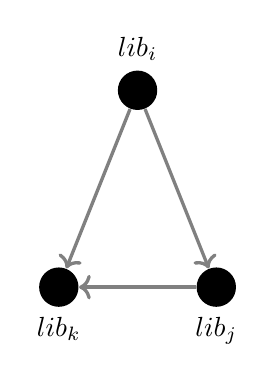
\begin{tikzpicture}[
         roundnode/.style={circle, fill=black, minimum size=5mm},
        squarenode/.style={fill=black, text=red, minimum size=5mm},
     ]
    \begin{scope}
         \node[roundnode, label=above:$lib_i$] (s2_proji) at (3, 2.5) {};
        \node[roundnode, label=below:$lib_j$] (s2_projj) at (4,0) {};
         \node[roundnode, label=below:$lib_k$] (s2_projk) at (2,0) {};
     \end{scope}

     \begin{scope} [every edge/.style={draw=gray, very thick}]
         \path [->] (s2_proji) edge (s2_projj);
         \path [->] (s2_proji) edge (s2_projk);
         \path [->] (s2_projj) edge (s2_projk);
     \end{scope}
     \end{tikzpicture}
    
     \caption{Example dependency graph for a given time period}
     \label{fig:lib}
     \vspace{2ex}
 \end{figure}
\begin{figure}[t]
    \centering

    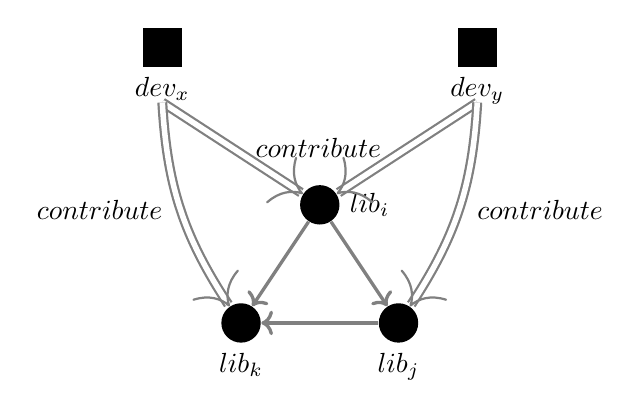
\begin{tikzpicture}[
        roundnode/.style={circle, fill=black, minimum size=5mm},
        squarenode/.style={fill=black, text=red, minimum size=5mm},
    ]
    \begin{scope}
        
        \node[roundnode, label=right:$lib_i$] (s2_proji) at (4, 1.5) {};
        \node[roundnode, label=below:$lib_j$] (s2_projj) at (5,0) {};
        \node[roundnode, label=below:$lib_k$] (s2_projk) at (3,0) {};
        
        \node[squarenode, label=below:$dev_x$] (s3_devx) at (2, 3.5) {};
        
        \node[squarenode, label=below:$dev_y$] (s3_devy) at (6, 3.5) {};
        
    \end{scope}

    \begin{scope} [every edge/.style={draw=gray, very thick}]
        \path [->] (s2_proji)  edge  (s2_projj);
        \path [->] (s2_proji) edge (s2_projk);
        \path [->] (s2_projj) edge (s2_projk);
        
    \end{scope}
    \begin{scope} [every edge/.style={draw=gray, thick, double distance=2pt}]
        \path [->] (6, 2.8) edge node[left = 2mm] {$contribute$} (s2_proji);
        \path [->] (6, 2.8) edge[bend left=15] node[right = 1mm] {$contribute$} (s2_projj);
        \path [->] (2, 2.8) edge node[right = 2mm] {$$} (s2_proji);
        \path [->] (2, 2.8) edge[bend right=15] node[left = 1mm] {$contribute$} (s2_projk);
    \end{scope}
    \end{tikzpicture}
\end{figure}
\begin{figure}[t]
    \centering
    \begin{tikzpicture}[
        roundnode/.style={circle, fill=black, minimum size=5mm},
        squarenode/.style={fill=black, text=red, minimum size=5mm},
    ]
    \end{tikzpicture}
\caption{Example Dependency-Contribution graph showing relationships between contributions and dependencies}
 \label{fig:dc-graph}
\end{figure}

This is just one example of the type of research that is enabled by access to heterogeneous data related to software package ecosystems.

\smallskip\noindent\textbf{Peril 1.}\textit{
 Developers might use different identifiers when contributing to different parts of a software package ecosystem, e.g., when contributing to different libraries.}\\
 
When modelling using such graphs, there is a threat that contributors may use multiple identifiers (i.e., $c_x$ and $c_y$ are the same contributor).
This is a well-known research problem, and there has been work to merge these accounts, such as \cite{wiese2016mailing}.
GitHub has introduced mechanisms such as two-factor authentication\footnote{\url{https://docs.github.com/en/authentication/securing-your-account-with-two-factor-authentication-2fa/configuring-two-factor-authentication}} to counteract the issue of multiple identifiers.
This is since developers might be less likely to switch accounts if it requires cumbersome authentication.


\smallskip\noindent\textbf{Peril 2.}\textit{
Developers' contributions to software package ecosystems might be interspersed with bot contributions, e.g., automated dependency updates.}\\

The rise of automation and artificial intelligence has led to much work on the integration of automated scheduling (i.e., bots) into software development workflows \cite{Storey2016, Farooq2016, Wessel2018, Erlenhov2019, bot_modify_wf} to name a few. These bots are designed to perform specific tasks within a software package ecosystem. For example, a bot may be programmed to automatically update dependencies, test code changes, or deploy software to production. As an example, the Google APIs repo-automation-bots project lists bots for automated labelling of issues and pull requests, automated approval of pull requests, and triggering releases.\footnote{\url{https://github.com/googleapis/repo-automation-bots}}
Bots perform common maintenance tasks in many software projects and are now commonplace \cite{Beschastnikh2017, Urli2018,BIMAN,bot_or_not}.
Especially with bots such as dependabot (automated pull requests to update configurations to reduce the risk of vulnerability threats),\footnote{\url{https://github.com/dependabot}} more and more automation has caused a lot of noise in the contributions between projects.
There are also bots for communication and documentation \cite{Urli2018, Lin2016, Lebeuf2017a}.

To be able to draw accurate conclusions about what humans are doing in software package ecosystems, researchers should consider distinguishing between bot and human contributions.
It is also important to differentiate this from other contributions \cite{maeprasart2022understanding}.
The research community has responded well, with a wide range of techniques and tools to mitigate this peril \cite{Bodegha2021, golzadeh2022accuracy}.

\smallskip\noindent\textbf{Peril 3.}\textit{
Not all developer activities in software package ecosystems are accessible to the public, e.g., library use in proprietary settings.
}\\

Not all developer activities in software package ecosystems are accessible to the public, e.g., when the boundary between open source and industry is blurred \cite{stol2014inner}, which presents a challenge for researchers who aim to study the development process. This is particularly true in proprietary settings where software development is performed behind closed doors or is open source for a limited time period, thus resulting in the artefacts not permanently being publicly available.
This can make it difficult to understand the broader ecosystem in which a software project is developed.
Proprietary settings may lead to non-standardisation in software development practises. Different software projects may use different management systems and tools, making it difficult to accurately compare and analyse software development activities across various projects. For example, some projects may use communication, documentation, and other management tools not captured on the same platform \cite{montgomery2022alternative}. For example, some projects might use Bugzilla instead of issues and pull requests for their bug and code review systems, while others may use Discord, Slack channels, or email threads for their communication needs.

This lack of standardisation in software development practises presents a challenge for researchers who study the software package ecosystem and understand the development process. To address this issue, researchers should strive to collect data from a diverse set of projects to gain a comprehensive understanding of the software package ecosystem. In addition, researchers may need to adjust their methodologies or data collection techniques to accommodate the different tools and practises used by different software projects.

\subsection{Defining Components and their Dependencies}

\smallskip\noindent\textbf{Promise 2.}\textit{
Researchers can access a software package ecosystem's dependency network through package managers and registries, e.g., npm lists the dependencies and dependents for over a million libraries.}\\


With the rise of curated datasets like libraries.io, researchers can now recover and model dependency relations between software units using pre-extracted datasets.
Table \ref{tab:PM_features} shows examples of popular package managers mined from the libraries.io dataset in 2020. 

\begin{table*}[]
\caption{Summary of 13 package managers from libraries.io as ranked by TIOBE in 2020}
 \label{tab:PM_features}
 \centering
\begin{tabular}{@{}llrlll@{}}
\toprule
\begin{tabular}[c]{@{}l@{}}Package \\ Ecosystem\end{tabular} & \begin{tabular}[c]{@{}l@{}}Programming \\ Language\end{tabular} &  \begin{tabular}[c]{@{}l@{}}Tiobe \\ Rank\end{tabular} & Environment & \begin{tabular}[c]{@{}l@{}}Dependency \\ Tree\end{tabular} & \begin{tabular}[c]{@{}l@{}}Package   \\Archive link\end{tabular}\\ \midrule
PyPI & Python & 2 & Python & Flat & pypi.org  \\
Maven & Java & 3 & JVM & Flat & Maven.org  \\
Bower & JavaScript & 7 & Node.js & Flat & bower.io  \\
Meteor & JavaScript & 7 & Node.js & Nested & atmospherejs.com \\
npm & JavaScript & 7 & Node.js & Nested (v2) & npmjs.com  \\
Packagist & PHP & 8 & PHP & Flat & packagist.org \\
Puppet & Ruby & 13 & Ruby MRI & Flat & forge.puppet.com  \\
RubyGems & Ruby & 13 & Ruby MRI & Flat & rubygems.org  \\
CRAN & R & 14 & RStudio & Flat & cran.r-project.org  \\
CPAN & Perl & 15 & Perl & Flat & metacpan.org  \\
GO & Golang & 20 & Go & Flat & pkg.go.dev  \\
NuGet & C\#, VB & 5, 6 & .NET & Flat & nuget.org \\
Anaconda & Python, R, C\# & 2, 14, 5 & Anaconda & Flat & anaconda.org  \\ \bottomrule
\end{tabular}
\end{table*}

\smallskip\noindent\textbf{Peril 4.}\textit{
Different software package ecosystems define the concept of ``dependency'' differently, e.g., by allowing or not allowing different versions of a library on the same dependency tree.
}\\

Different software package ecosystems have varying definitions of what constitutes a dependency. For example, some ecosystems may allow multiple versions of a library to exist on the same dependency tree, while others may restrict developers to a single version of a library \cite{Islam}. These restrictions are often based on the programming language being used, as different languages have different approaches to managing dependencies. It is important to consider the restrictions on dependency relationships when studying software package ecosystems, as they can have a major impact on the development process. For example, the ability to use multiple versions of a library on the same dependency tree can greatly simplify the process of updating dependencies and can make it easier to resolve conflicts between libraries.

One way to visualise the impact of these restrictions is to compare the difference between a nested dependency tree and a directed dependency tree, as shown in Figure \ref{fig:nest}.\footnote{Taken from \url{https://npm.github.io/how-npm-works-docs/npm3/how-npm3-works.html}} This distinction is important because it highlights the different ways that a software unit can depend on different versions of the same library.
In this example, npm v3 creates the dependency tree based on the installation order, therefore flattening unnecessary nested dependencies (i.e., B v1.0 in cyan). This reduces the complexity of a nested tree by resolving some of the transitive dependencies (nested dependencies).

\begin{figure}
	\centering
	\includegraphics[width=.8\textwidth]{book/chapter-promisesandperils/pics/nestedv2.jpg}
	\caption{Difference between flat and nested dependencies}
	\label{fig:nest}
\end{figure}

\smallskip\noindent\textbf{Peril 5.}\textit{
Developers might declare a dependency to other parts of a software package ecosystem but not use it, e.g., because they failed to update its removal.
}\\

It is common for developers to declare dependencies on other parts of the software package ecosystem but not always use them. This can happen for various reasons, such as forgetting to remove the dependency after it is no longer needed. This can pose a challenge for researchers who are trying to extract dependencies from package managers, like those in configuration files, as there may be inconsistencies between the listed dependencies and what is actually being compiled and used by the code. This can lead to a biased understanding of the software package ecosystem and the relationships between software components.

To address this issue, there have been numerous efforts to track the actual library dependencies compiled and executed in software systems. These efforts aim to provide a more accurate understanding of the dependencies and the relationships between software components. For example, research has been conducted on the use of dynamic analysis to track compiled dependencies in real time and on the development of tools to automatically detect and track executed dependencies \cite{Zapata:ICSME2018, Ponta2018,Chinthanet:ASE2020}.

\subsection{Defining Boundaries and Completeness}

\smallskip\noindent\textbf{Promise 3.}\textit{
Researchers can use the boundaries of software package ecosystems to study communities of developers, e.g., developers contributing to and/or benefiting from the npm ecosystem.
}\\

Following Promise 2, the emergence of package managers has also led to studies that approximate software communities.
Using the libraries.io dataset, researchers were able to study projects that host libraries that use package managers.
Researchers have used this dataset to compare different library ecosystems \cite{kikas.2017,decan:emse:2019,CogoDown2019}.


\smallskip\noindent\textbf{Peril 6.}\textit{
Package managers do not always represent software package ecosystems, their communities, or their sub-communities, e.g., in cases where multiple package managers exist.
}\\

Package managers are a fundamental aspect of software package ecosystems, but do not always fully represent the complex relationships and interactions that occur within a community of developers and users, as shown in Table~\ref{tab:PM_features}. In some cases, multiple package managers exist for the same programming language, creating a complex landscape of software libraries and dependencies that are not always easily understood. For instance, Bower and Meteor manage npm libraries, which can lead to confusion and overlap in the management of dependencies.

Similarly, Java, Scala, Android, and other Java-based open source communities all use the Maven package manager, but each of these communities has its own unique set of libraries, dependencies, and development practises. Researchers should be aware of the limitations of package managers when studying software package ecosystems, and consider the broader context and relationships that exist within these communities. 

\smallskip\noindent\textbf{Peril 7.}\textit{
Lack of activity in parts of a software package ecosystem does not necessarily indicate project failure, e.g., when highly depended-upon libraries are feature-complete.
}\\

It is important to note that lack of activity in a part of a software package ecosystem does not always mean project failure \cite{coelho2017modern}. In some cases, highly relied-upon libraries that have reached feature-completeness may see little activity, but continue to be used by the software community. 

However, it is still important to consider the long-term sustainability of these libraries, especially given the rate at which technology and software development practises change. This has become a topic of interest in recent years, and researchers have explored best practises for sustaining open source projects and ensuring their continued success \cite{Ait2022,valiev2018ecosystem}. Understanding the factors that contribute to project sustainability is important to ensure the longevity and continued growth of software package ecosystems.

\smallskip\noindent\textbf{Peril 8.}\textit{
Sampling from a software package ecosystem is challenging since sub-setting might alter the dependency network, e.g., by breaking dependency chains.
}\\

Sampling from a package ecosystem is not straightforward, as the sample composition can be significantly affected due to missing dependency links between libraries. For instance, a subset of the ecosystem might alter the dependencies between libraries, leading to the breakdown of the dependency chains. This could lead to an incomplete picture of the software package ecosystem, leading to incorrect conclusions from a study. To minimise this risk, researchers should carefully consider the boundaries of their study and choose the appropriate sampling method based on the research questions and goals. For example, researchers could focus on popular, highly dependent, or risk-vulnerable aspects of the ecosystem as a starting point. 
For some ecosystems, the number of downloads, GitHub stars, and watchers are other aspects for the researcher to utilise.


\smallskip\noindent\textbf{Peril 9.}\textit{
Sampling from a software package ecosystem is challenging since the dependency network changes over time, e.g., when dependencies are added, removed, upgraded, or downgraded.
}\\

The dynamic nature of package ecosystems and the constant changes to their dependencies can impact the generalisability of the results. Therefore, it is important to also consider the time granularity of the analysis. For example, if the goal is to understand the evolution of dependencies over time, a finer time granularity may be necessary to capture the smaller changes and trends. However, if the goal is to understand the overall structure and relationships within the ecosystem, a coarser time granularity may be sufficient. Based on recent studies \cite{wattanakriengkrai2022giving,valiev2018ecosystem,Mirsaeedi:icse2020, Brindescu:emse2020, Nassif:icsme2017}, a three-month window seems appropriate for some studies.
Another level of granularity to consider is the size of the component. For instance, there are cases where a single package may contain more than one repository, especially for large library frameworks. 
The granularity also depends on the nature of the ecosystem itself. For instance, researchers should understand whether the ecosystem comprises library packages (e.g., PyPI), plugins (e.g., Eclipse), or is a library distribution (e.g., Android).



\subsection{Analysing and Visualising the Data}

\textbf{Peril 10.}\textit{
Analysing and visualising entire software package ecosystems is challenging due to their size, e.g., in terms of nodes and edges in the network.
}\\

The size of software package ecosystems implies large data sets, which can be overwhelming for tools and algorithms to analyse and display. Therefore, it may be necessary to make choices about the granularity of the data included in the analysis and visualisation. Another alternative is to focus on the most critical parts of the software package ecosystem, such as the high-level structure, highly dependent packages, or parts of the system that pose a risk to security and reliability. 
The key is to strike a balance between detail and simplicity, providing a meaningful representation of the ecosystem while being able to handle the complexity of its size.


\section{Application: When to Apply Which Peril}
\label{PPM:sec:application}

We include a disclaimer stating that not all perils are applicable to every mining situation. To demonstrate the practical application of our perils and their mitigation, we present two case studies that involve mining the software package ecosystem. Each case study has a distinct research objective and focusses on a specific dataset to be mined.

\subsection{Two Case Studies}
Table \ref{tab:cases} presents the two case studies we have selected for this analysis.
The \textit{first case} involves mining for contributions congruent to dependency updates \cite{wattanakriengkrai2022giving}. 
In this work, the authors mine GitHub repositories for Pull Requests and Issues that were submitted and merged congruent to dependency updates within the npm ecosystem. 
The \textit{second case} involves mining communication data for the Eclipse ecosystem \cite{Nugroho2021}. Although the second case does not mine for dependency relations (i.e., use relations),  we show that these perils still apply when mining for other relationships in an ecosystem.
Moreover, the second case studies the Eclipse ecosystem, which is a different dataset compared to the more popular GitHub dataset.

\subsection{Applying Perils and their Mitigation Strategies}
Table \ref{tab:perilsapp} provides a summary of the perils that can be applied to each of the case studies. We will now go into the details of mitigation strategies based on these perils. 
For better organisation and understanding, we have grouped the perils according to the four logical processes for mining.

\smallskip\noindent\textbf{Information to Mine}. 
The first set of mitigation strategies, which addresses perils 1-3, focusses on planning which information to mine. There are two primary strategies that researchers can employ:


\begin{enumerate}
    \item Researchers should use research tools and techniques to remove noise and other biases in the dataset, such as bot detection and the handling of multiple identities. This strategy was implemented in both case studies, as contributions and discussions often have the potential to involve bots or developers with multiple identities.
\item Depending on the research goals, researchers should recognise that not all contributions are equal and filter the dataset accordingly.
\end{enumerate}

We applied these two strategies to both cases. In the first case, the goal was to capture all congruent contributions, so we filtered out contributions made to libraries without dependencies. Since all npm packages are listed in the registry, Peril 3 (private activities) did not apply.
In the second case, we addressed Peril 1 by conducting a qualitative analysis to ensure that the member identities were not duplicated, as Eclipse developers were known to change identities. To mitigate Peril 2, we removed bot responses. For the second case, since all forum data is made public, Peril 3 did not apply.


\begin{table}
\centering
\caption{Description of the research objectives and datasets for the case studies}
 \label{tab:cases}
\begin{tabular}{lp{5cm}r} 
\toprule
\textbf{Case Study} & \textbf{Research Objective}                                                          & \textbf{Datasets}           \\
\midrule
Wattanakriengkrai \etal \cite{wattanakriengkrai2022giving}             & Explore code contributions between library and client (i.e, use-relations)  & libraries.io\\
& &  GitHub API \\
Nugroho \etal \cite{Nugroho2021}                & Explore discussion contributions between contributors (i.e., contributions) & Eclipse API                \\
\bottomrule
\end{tabular}
\end{table}

\begin{table}
\centering
\caption{Application of each peril to the case studies}
 \label{tab:perilsapp}
\begin{tabular}{rp{8cm}ccc} 
\toprule                   
& \textbf{Perils}       & case 1      & case 2                 \\
                                                                               & & npm  & Eclipse   \\
\midrule
\textbf{P1} &Developers might use different identifiers when contributing to different parts of a software package ecosystem, e.g., when contributing to different libraries.                             &    \CheckedBox         &          \CheckedBox           \\ 
%\hline
\textbf{P2} & Developers' contributions to software package ecosystems might be interspersed with bot contributions, e.g., automated dependency updates.                                                      &      \CheckedBox               &      \CheckedBox               \\ 
%\hline
\textbf{P3} & Not all developer activities in software package ecosystems are accessible to the public, e.g., library use in proprietary settings.                                                         &         -           &      \CheckedBox               \\ 
%\hline
\textbf{P4} & Different software package ecosystems define the concept of \`{}\`{}dependency'' differently, e.g., by allowing or not allowing different versions of a library on the same dependency tree. &         \CheckedBox       &     -                            \\ 
%\hline
\textbf{P5} & Developers might declare a dependency to other parts of a software package ecosystem but not use it, e.g., because they failed to update its removal.                                        &     -           &  -    \\
%\hline
\textbf{P6} &Package managers do not always represent software package ecosystems, their communities, or their sub-communities, e.g., in cases where multiple package managers exist.                     &     -                   &  -                  \\
%\hline
\textbf{P7} & Lack of activity in parts of a software package ecosystem does not necessarily indicate project failure, e.g., when highly depended-upon libraries are feature-complete.                     &       \CheckedBox         &  -                           \\
%\hline
\textbf{P8} &Sampling from a software package ecosystem is challenging since sub-setting might alter the dependency network, e.g., by breaking dependency chains.                                         &        \CheckedBox        &     \CheckedBox                                \\
%\hline
\textbf{P9} &Sampling from a software package ecosystem is challenging since the dependency network changes over time, e.g., when dependencies are added, removed, upgraded, or downgraded.               &       \CheckedBox         &     -                          \\
%\hline
\textbf{P10} &Analysing and visualising entire software package ecosystems is challenging due to their size, e.g., in terms of nodes and edges in the network.                                  &        \CheckedBox      &      \CheckedBox               \\
\bottomrule
\end{tabular}
\end{table}

\smallskip\noindent\textbf{Defining Dependencies}. 
The second set of perils (Perils 4-5) is related to dependency relationships between software units, and only the first case study is applicable. To address these perils, researchers should adopt the following strategy:

\begin{enumerate}
    \item Researchers should not rely solely on listed dependencies in configuration files (e.g., pom.xml, package.json, etc.) as a measure of dependency between two components. Instead, code-centric approaches should be used to validate which libraries are actually depended upon.
\end{enumerate}

For example, in the first case, in addition to mining the configuration information, the authors also analysed the similarity of the source code contributions to address Peril 4. Regarding Peril 5, since the study's objective was to investigate changes to the configuration files, the risk of the update not being executed was deemed less important.
It is important to note that the second case study did not include dependency analysis and, therefore, these perils did not apply.

\begin{figure*}[]
    \centering
    \begin{subfigure}{0.9\linewidth}
         \includegraphics[width=1.1\textwidth]{book/chapter-promisesandperils/pics/congruentViz.jpg}
         \caption{Visualization of a Time analysis for 107,242 libraries.}
     \end{subfigure}
     \begin{subfigure}{0.9\linewidth}
         \includegraphics[width=1\textwidth]{book/chapter-promisesandperils/pics/eclipseViz.jpg}
         \caption{A Visual Topology map for 832,058 threads}
     \end{subfigure}
    \caption{Visualisation examples for the two case studies}
    \label{fig:visCase}
\end{figure*}

\smallskip\noindent\textbf{Defining Boundaries}.
The third set of perils (Perils 6-9) is related to the definition of boundaries and completeness and is relevant for both case studies. To mitigate these perils, we recommend the following strategies:

\begin{enumerate}
    \item Researchers should recognise that a dormant project does not necessarily mean that it is inactive. Instead, studies can use alternative heuristics, such as the number of dependents and dependencies, as better indicators of a project's importance in the ecosystem.
    \item Researchers should not rely solely on the programming language to define sub-communities. Using a common package manager for the programming language is a more effective rule of thumb for distinguishing boundaries.
    \item Researchers should avoid random sampling. Instead, sampling should be tailored to the research goals by considering factors such as an appropriate time window or focussing on specific attributes of components (e.g., most dependents, most popular, most contributors).
\end{enumerate}


Peril 6 did not apply to any of the case studies. 
Particularly for the first case, since the goal was to explore the npm package ecosystem, we assumed that the boundaries were clearly defined by the npm registry. 
Similarly, the second case study used the generic Eclipse platform as the boundary. 
Peril 7 was applied to the npm study, while Peril 8 was applied to both case studies. 
As a result, the two cases conducted a qualitative analysis of the dataset to gain deeper insights.
In the first case study, a three-month time window was created to capture dependencies. 
For the second case study, forum contributors were sampled into three groups (i.e., junior, member, or senior) according to the sliding window of their contributions. 

\smallskip\noindent\textbf{Visualisation}.
The final peril (Peril 10) relates to visualisation, which can be challenging due to the vast size and complexity of software ecosystems. As it is not feasible to visualise every aspect of an ecosystem simultaneously, a focused approach is necessary. A mitigation strategy is to select specific attributes of the ecosystem (e.g., the most dependent, most popular, and most contributions) that align with the research needs and objectives. 

Figure \ref{fig:visCase} shows two cases where visualizations are employed to gain insights, especially for large datasets.
In the first figure (a), we visualize the distributions of the data set and applied the appropriate statistical tests, along with the effect size, to test our hypotheses and answer research questions. 
In the second example (b), although not directly related to package ecosystems, the authors utilized a topological visualization \cite{Lum2013ExtractingIF} to gain insights on the over 800,000 forum threads of discussions. 



\section{Chapter Summary}
In this chapter, we explore the various aspects of mining information from the software package ecosystem, presenting three promises and ten perils that researchers should be aware of when undertaking such tasks. The chapter is structured around four key processes for mining: 1) Planning what Information to Mine, 2) Defining Components and their Dependencies, 3) Defining Boundaries and Completeness, and 4) Analysing and Visualising the Data. To help new and experienced researchers navigate these challenges, we introduced the SUG model, which can serve as a valuable tool to minimise threats to validity. Although some perils may be more relevant to specific research objectives, our aim is to equip researchers with the knowledge and resources needed to confidently gather and integrate software package ecosystem data into their work.
 %Managing modeling ecosystems by means of machine learning techniques
% %Semantic labeling three-letter-code: MDE (e.g. \chapter{MDE})

% 
\title{Promises and Perils of Mining \\ Software Package Ecosystem Data}
\author{Raula Gaikovina Kula \and Katsuro Inoue \and Christoph Treude}
\institute{Raula Gaikovina Kula \at Nara Institute of Science and Technology, Japan, \email{raula-k@naist.jp}
\and Katsuro Inoue \at Nanzan University, Japan \email{ inoue599@nanzan-u.ac.jp}
\and  Christoph Treude \at The University of Melbourne, Australia \email{christoph.treude@unimelb.edu.au}}

\maketitle
\label{PPM:ch}
\abstract*{The use of third-party packages is becoming increasingly popular and has led to the emergence of large software package ecosystems with a maze of inter-dependencies. Since the reliance on these ecosystems enables developers to reduce development effort and increase productivity, it has attracted the interest of researchers: understanding the infrastructure and dynamics of package ecosystems has given rise to approaches for better code reuse, automated updates, and the avoidance of vulnerabilities, to name a few examples. But the reality of these ecosystems also poses challenges to software engineering researchers, such as: How do we obtain the complete network of dependencies along with the corresponding versioning information? What are the boundaries of these package ecosystem? How do we consistently detect dependencies that are declared but not used? How do we consistently identify developers within a package ecosystem? How much of the ecosystem do we need to understand to analyse a single component? How well do our approaches generalise across different programming languages and package ecosystems? In this chapter, we review promises and perils of mining the rich data related to software package ecosystems available to software engineering researchers.}

\abstract{The use of third-party packages is becoming increasingly popular and has led to the emergence of large software package ecosystems with a maze of inter-dependencies. Since the reliance on these ecosystems enables developers to reduce development effort and increase productivity, it has attracted the interest of researchers: understanding the infrastructure and dynamics of package ecosystems has given rise to approaches for better code reuse, automated updates, and the avoidance of vulnerabilities, to name a few examples. But the reality of these ecosystems also poses challenges to software engineering researchers, such as: How do we obtain the complete network of dependencies along with the corresponding versioning information? What are the boundaries of these package ecosystems? How do we consistently detect dependencies that are declared but not used? How do we consistently identify developers within a package ecosystem? How much of the ecosystem do we need to understand to analyse a single component? How well do our approaches generalise across different programming languages and package ecosystems? In this chapter, we review promises and perils of mining the rich data related to software package ecosystems available to software engineering researchers.}

%%%%%%%%%%%%%%%%%%%%%%%%%%%%%%%%%%%%%%%%%%%%%%%%%%%%%%%%%%%%%%%%%%

\section{Introduction}
\label{PPM:sec:definition}

Third-party libraries are a great way for developers to incorporate code without having to write their own for every functionality required. By using these libraries, developers can save time and energy while still getting the functions they need.
Using third-party libraries is becoming increasingly popular and has led to the emergence of large software package ecosystems such as npm. While these ecosystems offer many benefits, they also come with risks, such as software vulnerability attacks \cite{Chinthanet:ASE2020}.

Large software package ecosystems are a treasure trove for researchers who can investigate a wide range of questions. For example, by studying activity in large ecosystems, researchers can identify which libraries are the most popular and learn what characteristics make them successful \cite{kikas.2017,decan:emse:2019}.
Additionally, research on large ecosystems can help developers understand how to protect their code from malicious actors who may attempt to exploit vulnerabilities or insert malware into popular libraries.
Studying large software package ecosystems can help us better understand the dynamics of open source development in general. Open source development is a complex process that involves many different stakeholders working together (or sometimes competing) to create valuable code that anyone can use or improve upon. By understanding how these interactions play out in different types of ecosystem structures -- including those with many small projects versus few very large ones -- we can develop insights that might be applicable more broadly across other types of collaborative systems.

In this chapter, we identify and discuss promises and perils during the mining process, ranging from planning what information to mine from the ecosystem to analysing and visualising the mined data. 
Therefore, the chapter is broken down into these logical processes of mining ecosystem data: 1) Planning what Information to Mine, 2) Defining Components and their Dependencies, 3) Defining Boundaries and Completeness, and 4) Analysing and Visualising the Data.

This chapter is intended for researchers and practitioners who are interested in exploring and exploiting software package ecosystem information from a diverse range of sources that are publicly available. 
We also highlight the pitfalls to consider during the mining process, particularly when these pitfalls could lead to a misinterpretation of the analysis and results. 
The chapter is written in a manner that encourages newcomers who have little or no experience or who are interested in utilising ecosystem data across different disciplines outside of software engineering.
Our goal is to get new researchers quickly accustomed to gathering ecosystem information for their research.


\section{A Component-based Software Ecosystem}

Defined as a component-based software ecosystem, we suggest using the term `software package ecosystem' as a suitable term for the symbiotic relationships among third-party library components (as software projects or repositories), as these libraries and their dependent clients coexist on the same technological platform, therefore sharing the same environment and other internal and external factors (e.g., security threats, sharing contributions, etc.).
Please refer to the Introduction chapter for an in-depth definition of the different types of software ecosystems.
We present our interpretation of the software package ecosystem in Kula et al.~\cite{KulaSANER18}, where we formally define a package ecosystem using a Software Universe Graph (SUG).
This is modelled as a structured abstraction of the evolution of software systems and their library dependencies over time.

%%%%%%%%%%%%%%%%%%%%%%%%%%%%%%%%%%%%%%%%%%
\begin{figure*}
	\centering
	\includegraphics[width=.7\textwidth]{book/chapter-promisesandperils/pics/UniversalExample.jpg}
	\caption{Conceptual example of the Software Universe Graph, depicting the use and update relationships between different software units.}
	\label{fig:SUG}
\end{figure*}
%%%%%%%%%%%%%%%%%%%%%%%%%%%%%%%%%%%%%%%%%%%%%


\paragraph{\textbf{Component-based Representation as a Software Universe Graph}}
\label{PPM:sec:SUG}

First introduced by Kula et al.~\cite{KulaSANER18}, the \textit{Software Universe Graph} (SUG) is a structural abstraction of the software ecosystem of third-party libraries.
Figure \ref{fig:SUG} provides an illustration of the different relationships within the graph.
Let $G= (N,E)$ represent a graph $G$. $N$ is a set of nodes, each node representing a software unit. 
We define a software unit as a version instance of any software program. 

The authors then present the \textit{use} and \textit{update} relationships that exist in the ecosystem.
Hence, the edges $E$ are composed of $E_{use}$ and $E_{update}$. $E_{use}$ is a set of \textit{use-relations} and $E_{update}$ is a set of \textit{update-relations}.

\begin{definition}
An edge $u \rightarrow v \in E_{use}$ means that $u$ uses $v$. The defined functions of $E_{use}$ are:

\begin{equation}
\small
\small \use(u)\equiv \{v|u \rightarrow v\}
\normalsize
\end{equation}
\begin{equation}
\small
\small \useBy(u)\equiv \{v|v \rightarrow u\}
\normalsize
\end{equation}
\end{definition}

Use-relations can be extracted from either the source code or configuration files. 
As shown in Figure \ref{fig:SUG}, node $a1$ uses node $x1$. 
In addition, node $x1$ is used by nodes $a1$, $q1$, and $q2$. Parallel edges for node pairs are not allowed.

\begin{definition}
We represent an update relation from node $a$ to $b$ using $ a \Rightarrow b $, which means that the newer update $b$ was released from node $a$ and is defined as:
\begin{equation}
\small a \Rightarrow b \in E_{update}
\end{equation}
\end{definition}

Update relations refer to when a successive release of a software unit is made available. Figure \ref{fig:SUG} shows that node $q1$ is first updated to node $q2$. Later, node $q2$ is updated to the latest node $q3$. Hence, $q1 \Rightarrow q2 \Rightarrow q3$.
Note that an update should not be confused with forking. 
We distinguish a fork as a separate software unit. 
Each node in the SUG should be denoted by three attributes: \texttt{<name,release,time>}.  
For a node $u$, we define:

\begin{itemize}
	\item \textbf{u.name} Name is the string representation identifier of a software unit.
	We introduce the name axiom: For nodes $u$ and $v$, if $u \Rightarrow v$, then $u.name = v.name$ holds.
	
	\item \textbf{u.release}. Release refers to the specific assigned change reference for a software unit. For nodes $u$ and $v$, if $u \Rightarrow v$
	then $v$ is the immediate successor of $u$. Note that the versioning pattern may vary from project to project. 
	\item \textbf{u.time}. Time refers to the time stamp at which node $u$ was released. For nodes $u$ and $v$ of $u \Rightarrow v$, $u.time < v.time$.
\end{itemize}

\begin{figure}
	\centering
	\includegraphics[width=.8\textwidth]{book/chapter-promisesandperils/pics/TemporalSUG.jpg}
	\caption{Temporal property of the SUG}
	\label{fig:SUGTemp}
\end{figure}

\begin{definition}
    
	The SUG has temporal properties.
This describes the simultaneity or ordering in reference to time. Let SUG $G = (N, E) $ be at time $t$. At time $t^{\prime} > t$, we observe an extension of $G$, such that:

\begin{equation}
\small G^{\prime} = (N \cup \Delta N, E \cup \Delta E)
\end{equation}
where $\Delta E \cap (N \times N) = \emptyset$
\end{definition}

Figure \ref{fig:SUGTemp} illustrates the temporal properties of the SUG. 
Here, it is observed that $G'$ is composed of $G$ augmented with newly added node $a3$ and its corresponding $a3 \rightarrow x2$ and $a2 \Rightarrow a3$ relations.
A SUG grows monotonically over time with only additions.
Here, we consider that modification or deletion changes on the SUG do not occur. 

\begin{definition}
    A timed SUG specifies the state of the SUG at any point in time.
So for an SUG $G=(N,E)$, we represent a timed SUG $G_{t}$ at time $t$ as a sub-graph of $G$. Formally,
\begin{equation}
\small G_t\equiv(N_{t}, E_{t})
\end{equation}
where $N_{t} = \{u|u \in N, u.time \leq t \}$ and $E_t = \{ e | e \in E \wedge e \in  N_t \}$
\end{definition}
	


\section{Data Sources}
Researchers can use various datasets to model the ecosystem using the SUG model of usage and update relationships.
The most obvious data source that has revolutionised data mining in the software engineering domain is the GitHub platform. 
Established in 2008, and then purchased by Microsoft in 2020, GitHub is home to various popular Open Source Software. 
GitHub is built on the git version control system and is useful for storing all changes made to a repository. 
In the case of the SUG, a GitHub repository can represent one software unit, whose depend relations can be extracted via a configuration file (such as the package.json file for JavaScript projects).
The repository should also contain the release information that holds the update relations.
Due to its large size, researchers and the GitHub team have made available datasets for researchers to mine, for example through the GitHub API/Graph QL.\footnote{\url{https://docs.github.com/en/graphql}} This is the backend Application Programming Interface (API) that can be used to query large amounts of data on GitHub. Most researchers use the API to download and mine information from the GitHub platform. 
It is important to note that while GitHub introduced a new feature of Dependency Graphs to map the depend relationship,\footnote{\url{https://docs.github.com/en/code-security/supply-chain-security/understanding-your-software-supply-chain/about-the-dependency-graph}} most older projects do not have this feature.
In this case, the researcher would need to manually extract and query the configuration files for dependency information. 

We refer to the first chapter for additional information on data sources for mining software ecosystems. 

\section{Promises and Perils}
\label{PPM:sec:promisesperils}

Using the SUG model of depend and use relations and the available datasets, we can now present our promises and perils of mining ecosystem information.

\subsection{Planning What Information to Mine}

\textbf{Promise 1.}\textit{
Researchers can access and link heterogeneous data related to software package ecosystems, e.g., package registries and bug trackers.}\\

When planning what information to mine from the ecosystem, researchers do not need to limit themselves to the usage and update relationship information.
Platforms that host software repositories include other software management systems such as bug trackers.
For example, GitHub allows researchers to manage GitHub Pull Requests, Issues, and Discussions not only for one project, but for multiple projects.
GitHub provides three management systems that are related to a software repository:

\begin{itemize}
    \item \textit{GitHub Discussions}\footnote{\url{https://docs.github.com/en/discussions}} - The GitHub Discussions forum is a collaborative communication forum for the community around an open source or internal project. Community members can ask and answer questions, share updates, have open-ended conversations, and follow along on decisions affecting the community's way of working.
    \item \textit{GitHub Pull Requests}\footnote{\url{https://docs.github.com/en/pull-requests}} - Pull Requests allow other developers from an ecosystem to make a contribution to a software repository. Pull requests also allow maintainers to discuss and review potential changes with collaborators and add follow-up commits before changes are merged into the software.
    \item \textit{GitHub Issues}\footnote{\url{https://docs.github.com/en/issues}} - Issues are used to track ideas, feedback, tasks, or bugs for work on GitHub.
\end{itemize}

These three systems are examples of how developers contribute to both their own and other projects. 
Hence, to incorporate this information, we can extend the SUG model, creating a model that includes a contribution relationship \cite{wattanakriengkrai2022giving}.

% Note that other platforms may also have management systems, like GitLab, BitBucket and Eclipse.

\begin{definition}
	A Dependency-Contribution graph incorporates contributions by developers whose libraries are involved in dependency relationships. 
\end{definition}

In this work \cite{wattanakriengkrai2022giving}, the authors explore the congruence between dependency updates and developer contributions, based on the original concept of social-technical congruence \cite{stcCataldo2008} where developers contribution patterns are congruent with their coordination needs. Hence, the goal is to identify contributions that are congruent to dependency updates.
As shown in Figure \ref{fig:lib} the authors extend from the typical SUG graph model where $lib_i$ depends (use) on  $lib_k$ and  $lib_j$, while  $lib_j$ also depends on $lib_k$, to the example shown in Figure \ref{fig:dc-graph}.
Different to the SUG, the graph captures developers and their contributions (i.e., the square as $dev_x$ and $dev_y$ represent two different developers making a contribution).
Here contributions are defined as $c$ (Pull Request or Issue) that were submitted to both a library and the client that depends on that library.
Hence, the graph can show contributions that are congruent to dependency changes for a software unit. 

\begin{figure}[t]
     \centering
     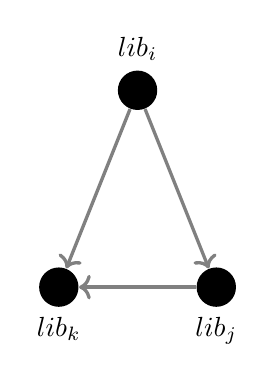
\begin{tikzpicture}[
         roundnode/.style={circle, fill=black, minimum size=5mm},
        squarenode/.style={fill=black, text=red, minimum size=5mm},
     ]
    \begin{scope}
         \node[roundnode, label=above:$lib_i$] (s2_proji) at (3, 2.5) {};
        \node[roundnode, label=below:$lib_j$] (s2_projj) at (4,0) {};
         \node[roundnode, label=below:$lib_k$] (s2_projk) at (2,0) {};
     \end{scope}

     \begin{scope} [every edge/.style={draw=gray, very thick}]
         \path [->] (s2_proji) edge (s2_projj);
         \path [->] (s2_proji) edge (s2_projk);
         \path [->] (s2_projj) edge (s2_projk);
     \end{scope}
     \end{tikzpicture}
    
     \caption{Example dependency graph for a given time period}
     \label{fig:lib}
     \vspace{2ex}
 \end{figure}
\begin{figure}[t]
    \centering

    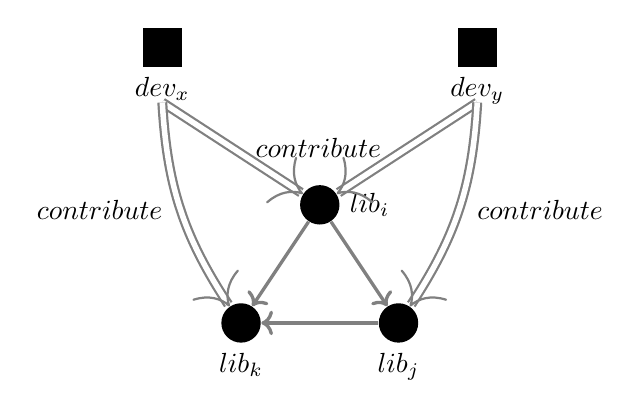
\begin{tikzpicture}[
        roundnode/.style={circle, fill=black, minimum size=5mm},
        squarenode/.style={fill=black, text=red, minimum size=5mm},
    ]
    \begin{scope}
        
        \node[roundnode, label=right:$lib_i$] (s2_proji) at (4, 1.5) {};
        \node[roundnode, label=below:$lib_j$] (s2_projj) at (5,0) {};
        \node[roundnode, label=below:$lib_k$] (s2_projk) at (3,0) {};
        
        \node[squarenode, label=below:$dev_x$] (s3_devx) at (2, 3.5) {};
        
        \node[squarenode, label=below:$dev_y$] (s3_devy) at (6, 3.5) {};
        
    \end{scope}

    \begin{scope} [every edge/.style={draw=gray, very thick}]
        \path [->] (s2_proji)  edge  (s2_projj);
        \path [->] (s2_proji) edge (s2_projk);
        \path [->] (s2_projj) edge (s2_projk);
        
    \end{scope}
    \begin{scope} [every edge/.style={draw=gray, thick, double distance=2pt}]
        \path [->] (6, 2.8) edge node[left = 2mm] {$contribute$} (s2_proji);
        \path [->] (6, 2.8) edge[bend left=15] node[right = 1mm] {$contribute$} (s2_projj);
        \path [->] (2, 2.8) edge node[right = 2mm] {$$} (s2_proji);
        \path [->] (2, 2.8) edge[bend right=15] node[left = 1mm] {$contribute$} (s2_projk);
    \end{scope}
    \end{tikzpicture}
\end{figure}
\begin{figure}[t]
    \centering
    \begin{tikzpicture}[
        roundnode/.style={circle, fill=black, minimum size=5mm},
        squarenode/.style={fill=black, text=red, minimum size=5mm},
    ]
    \end{tikzpicture}
\caption{Example Dependency-Contribution graph showing relationships between contributions and dependencies}
 \label{fig:dc-graph}
\end{figure}

This is just one example of the type of research that is enabled by access to heterogeneous data related to software package ecosystems.

\smallskip\noindent\textbf{Peril 1.}\textit{
 Developers might use different identifiers when contributing to different parts of a software package ecosystem, e.g., when contributing to different libraries.}\\
 
When modelling using such graphs, there is a threat that contributors may use multiple identifiers (i.e., $c_x$ and $c_y$ are the same contributor).
This is a well-known research problem, and there has been work to merge these accounts, such as \cite{wiese2016mailing}.
GitHub has introduced mechanisms such as two-factor authentication\footnote{\url{https://docs.github.com/en/authentication/securing-your-account-with-two-factor-authentication-2fa/configuring-two-factor-authentication}} to counteract the issue of multiple identifiers.
This is since developers might be less likely to switch accounts if it requires cumbersome authentication.


\smallskip\noindent\textbf{Peril 2.}\textit{
Developers' contributions to software package ecosystems might be interspersed with bot contributions, e.g., automated dependency updates.}\\

The rise of automation and artificial intelligence has led to much work on the integration of automated scheduling (i.e., bots) into software development workflows \cite{Storey2016, Farooq2016, Wessel2018, Erlenhov2019, bot_modify_wf} to name a few. These bots are designed to perform specific tasks within a software package ecosystem. For example, a bot may be programmed to automatically update dependencies, test code changes, or deploy software to production. As an example, the Google APIs repo-automation-bots project lists bots for automated labelling of issues and pull requests, automated approval of pull requests, and triggering releases.\footnote{\url{https://github.com/googleapis/repo-automation-bots}}
Bots perform common maintenance tasks in many software projects and are now commonplace \cite{Beschastnikh2017, Urli2018,BIMAN,bot_or_not}.
Especially with bots such as dependabot (automated pull requests to update configurations to reduce the risk of vulnerability threats),\footnote{\url{https://github.com/dependabot}} more and more automation has caused a lot of noise in the contributions between projects.
There are also bots for communication and documentation \cite{Urli2018, Lin2016, Lebeuf2017a}.

To be able to draw accurate conclusions about what humans are doing in software package ecosystems, researchers should consider distinguishing between bot and human contributions.
It is also important to differentiate this from other contributions \cite{maeprasart2022understanding}.
The research community has responded well, with a wide range of techniques and tools to mitigate this peril \cite{Bodegha2021, golzadeh2022accuracy}.

\smallskip\noindent\textbf{Peril 3.}\textit{
Not all developer activities in software package ecosystems are accessible to the public, e.g., library use in proprietary settings.
}\\

Not all developer activities in software package ecosystems are accessible to the public, e.g., when the boundary between open source and industry is blurred \cite{stol2014inner}, which presents a challenge for researchers who aim to study the development process. This is particularly true in proprietary settings where software development is performed behind closed doors or is open source for a limited time period, thus resulting in the artefacts not permanently being publicly available.
This can make it difficult to understand the broader ecosystem in which a software project is developed.
Proprietary settings may lead to non-standardisation in software development practises. Different software projects may use different management systems and tools, making it difficult to accurately compare and analyse software development activities across various projects. For example, some projects may use communication, documentation, and other management tools not captured on the same platform \cite{montgomery2022alternative}. For example, some projects might use Bugzilla instead of issues and pull requests for their bug and code review systems, while others may use Discord, Slack channels, or email threads for their communication needs.

This lack of standardisation in software development practises presents a challenge for researchers who study the software package ecosystem and understand the development process. To address this issue, researchers should strive to collect data from a diverse set of projects to gain a comprehensive understanding of the software package ecosystem. In addition, researchers may need to adjust their methodologies or data collection techniques to accommodate the different tools and practises used by different software projects.

\subsection{Defining Components and their Dependencies}

\smallskip\noindent\textbf{Promise 2.}\textit{
Researchers can access a software package ecosystem's dependency network through package managers and registries, e.g., npm lists the dependencies and dependents for over a million libraries.}\\


With the rise of curated datasets like libraries.io, researchers can now recover and model dependency relations between software units using pre-extracted datasets.
Table \ref{tab:PM_features} shows examples of popular package managers mined from the libraries.io dataset in 2020. 

\begin{table*}[]
\caption{Summary of 13 package managers from libraries.io as ranked by TIOBE in 2020}
 \label{tab:PM_features}
 \centering
\begin{tabular}{@{}llrlll@{}}
\toprule
\begin{tabular}[c]{@{}l@{}}Package \\ Ecosystem\end{tabular} & \begin{tabular}[c]{@{}l@{}}Programming \\ Language\end{tabular} &  \begin{tabular}[c]{@{}l@{}}Tiobe \\ Rank\end{tabular} & Environment & \begin{tabular}[c]{@{}l@{}}Dependency \\ Tree\end{tabular} & \begin{tabular}[c]{@{}l@{}}Package   \\Archive link\end{tabular}\\ \midrule
PyPI & Python & 2 & Python & Flat & pypi.org  \\
Maven & Java & 3 & JVM & Flat & Maven.org  \\
Bower & JavaScript & 7 & Node.js & Flat & bower.io  \\
Meteor & JavaScript & 7 & Node.js & Nested & atmospherejs.com \\
npm & JavaScript & 7 & Node.js & Nested (v2) & npmjs.com  \\
Packagist & PHP & 8 & PHP & Flat & packagist.org \\
Puppet & Ruby & 13 & Ruby MRI & Flat & forge.puppet.com  \\
RubyGems & Ruby & 13 & Ruby MRI & Flat & rubygems.org  \\
CRAN & R & 14 & RStudio & Flat & cran.r-project.org  \\
CPAN & Perl & 15 & Perl & Flat & metacpan.org  \\
GO & Golang & 20 & Go & Flat & pkg.go.dev  \\
NuGet & C\#, VB & 5, 6 & .NET & Flat & nuget.org \\
Anaconda & Python, R, C\# & 2, 14, 5 & Anaconda & Flat & anaconda.org  \\ \bottomrule
\end{tabular}
\end{table*}

\smallskip\noindent\textbf{Peril 4.}\textit{
Different software package ecosystems define the concept of ``dependency'' differently, e.g., by allowing or not allowing different versions of a library on the same dependency tree.
}\\

Different software package ecosystems have varying definitions of what constitutes a dependency. For example, some ecosystems may allow multiple versions of a library to exist on the same dependency tree, while others may restrict developers to a single version of a library \cite{Islam}. These restrictions are often based on the programming language being used, as different languages have different approaches to managing dependencies. It is important to consider the restrictions on dependency relationships when studying software package ecosystems, as they can have a major impact on the development process. For example, the ability to use multiple versions of a library on the same dependency tree can greatly simplify the process of updating dependencies and can make it easier to resolve conflicts between libraries.

One way to visualise the impact of these restrictions is to compare the difference between a nested dependency tree and a directed dependency tree, as shown in Figure \ref{fig:nest}.\footnote{Taken from \url{https://npm.github.io/how-npm-works-docs/npm3/how-npm3-works.html}} This distinction is important because it highlights the different ways that a software unit can depend on different versions of the same library.
In this example, npm v3 creates the dependency tree based on the installation order, therefore flattening unnecessary nested dependencies (i.e., B v1.0 in cyan). This reduces the complexity of a nested tree by resolving some of the transitive dependencies (nested dependencies).

\begin{figure}
	\centering
	\includegraphics[width=.8\textwidth]{book/chapter-promisesandperils/pics/nestedv2.jpg}
	\caption{Difference between flat and nested dependencies}
	\label{fig:nest}
\end{figure}

\smallskip\noindent\textbf{Peril 5.}\textit{
Developers might declare a dependency to other parts of a software package ecosystem but not use it, e.g., because they failed to update its removal.
}\\

It is common for developers to declare dependencies on other parts of the software package ecosystem but not always use them. This can happen for various reasons, such as forgetting to remove the dependency after it is no longer needed. This can pose a challenge for researchers who are trying to extract dependencies from package managers, like those in configuration files, as there may be inconsistencies between the listed dependencies and what is actually being compiled and used by the code. This can lead to a biased understanding of the software package ecosystem and the relationships between software components.

To address this issue, there have been numerous efforts to track the actual library dependencies compiled and executed in software systems. These efforts aim to provide a more accurate understanding of the dependencies and the relationships between software components. For example, research has been conducted on the use of dynamic analysis to track compiled dependencies in real time and on the development of tools to automatically detect and track executed dependencies \cite{Zapata:ICSME2018, Ponta2018,Chinthanet:ASE2020}.

\subsection{Defining Boundaries and Completeness}

\smallskip\noindent\textbf{Promise 3.}\textit{
Researchers can use the boundaries of software package ecosystems to study communities of developers, e.g., developers contributing to and/or benefiting from the npm ecosystem.
}\\

Following Promise 2, the emergence of package managers has also led to studies that approximate software communities.
Using the libraries.io dataset, researchers were able to study projects that host libraries that use package managers.
Researchers have used this dataset to compare different library ecosystems \cite{kikas.2017,decan:emse:2019,CogoDown2019}.


\smallskip\noindent\textbf{Peril 6.}\textit{
Package managers do not always represent software package ecosystems, their communities, or their sub-communities, e.g., in cases where multiple package managers exist.
}\\

Package managers are a fundamental aspect of software package ecosystems, but do not always fully represent the complex relationships and interactions that occur within a community of developers and users, as shown in Table~\ref{tab:PM_features}. In some cases, multiple package managers exist for the same programming language, creating a complex landscape of software libraries and dependencies that are not always easily understood. For instance, Bower and Meteor manage npm libraries, which can lead to confusion and overlap in the management of dependencies.

Similarly, Java, Scala, Android, and other Java-based open source communities all use the Maven package manager, but each of these communities has its own unique set of libraries, dependencies, and development practises. Researchers should be aware of the limitations of package managers when studying software package ecosystems, and consider the broader context and relationships that exist within these communities. 

\smallskip\noindent\textbf{Peril 7.}\textit{
Lack of activity in parts of a software package ecosystem does not necessarily indicate project failure, e.g., when highly depended-upon libraries are feature-complete.
}\\

It is important to note that lack of activity in a part of a software package ecosystem does not always mean project failure \cite{coelho2017modern}. In some cases, highly relied-upon libraries that have reached feature-completeness may see little activity, but continue to be used by the software community. 

However, it is still important to consider the long-term sustainability of these libraries, especially given the rate at which technology and software development practises change. This has become a topic of interest in recent years, and researchers have explored best practises for sustaining open source projects and ensuring their continued success \cite{Ait2022,valiev2018ecosystem}. Understanding the factors that contribute to project sustainability is important to ensure the longevity and continued growth of software package ecosystems.

\smallskip\noindent\textbf{Peril 8.}\textit{
Sampling from a software package ecosystem is challenging since sub-setting might alter the dependency network, e.g., by breaking dependency chains.
}\\

Sampling from a package ecosystem is not straightforward, as the sample composition can be significantly affected due to missing dependency links between libraries. For instance, a subset of the ecosystem might alter the dependencies between libraries, leading to the breakdown of the dependency chains. This could lead to an incomplete picture of the software package ecosystem, leading to incorrect conclusions from a study. To minimise this risk, researchers should carefully consider the boundaries of their study and choose the appropriate sampling method based on the research questions and goals. For example, researchers could focus on popular, highly dependent, or risk-vulnerable aspects of the ecosystem as a starting point. 
For some ecosystems, the number of downloads, GitHub stars, and watchers are other aspects for the researcher to utilise.


\smallskip\noindent\textbf{Peril 9.}\textit{
Sampling from a software package ecosystem is challenging since the dependency network changes over time, e.g., when dependencies are added, removed, upgraded, or downgraded.
}\\

The dynamic nature of package ecosystems and the constant changes to their dependencies can impact the generalisability of the results. Therefore, it is important to also consider the time granularity of the analysis. For example, if the goal is to understand the evolution of dependencies over time, a finer time granularity may be necessary to capture the smaller changes and trends. However, if the goal is to understand the overall structure and relationships within the ecosystem, a coarser time granularity may be sufficient. Based on recent studies \cite{wattanakriengkrai2022giving,valiev2018ecosystem,Mirsaeedi:icse2020, Brindescu:emse2020, Nassif:icsme2017}, a three-month window seems appropriate for some studies.
Another level of granularity to consider is the size of the component. For instance, there are cases where a single package may contain more than one repository, especially for large library frameworks. 
The granularity also depends on the nature of the ecosystem itself. For instance, researchers should understand whether the ecosystem comprises library packages (e.g., PyPI), plugins (e.g., Eclipse), or is a library distribution (e.g., Android).



\subsection{Analysing and Visualising the Data}

\textbf{Peril 10.}\textit{
Analysing and visualising entire software package ecosystems is challenging due to their size, e.g., in terms of nodes and edges in the network.
}\\

The size of software package ecosystems implies large data sets, which can be overwhelming for tools and algorithms to analyse and display. Therefore, it may be necessary to make choices about the granularity of the data included in the analysis and visualisation. Another alternative is to focus on the most critical parts of the software package ecosystem, such as the high-level structure, highly dependent packages, or parts of the system that pose a risk to security and reliability. 
The key is to strike a balance between detail and simplicity, providing a meaningful representation of the ecosystem while being able to handle the complexity of its size.


\section{Application: When to Apply Which Peril}
\label{PPM:sec:application}

We include a disclaimer stating that not all perils are applicable to every mining situation. To demonstrate the practical application of our perils and their mitigation, we present two case studies that involve mining the software package ecosystem. Each case study has a distinct research objective and focusses on a specific dataset to be mined.

\subsection{Two Case Studies}
Table \ref{tab:cases} presents the two case studies we have selected for this analysis.
The \textit{first case} involves mining for contributions congruent to dependency updates \cite{wattanakriengkrai2022giving}. 
In this work, the authors mine GitHub repositories for Pull Requests and Issues that were submitted and merged congruent to dependency updates within the npm ecosystem. 
The \textit{second case} involves mining communication data for the Eclipse ecosystem \cite{Nugroho2021}. Although the second case does not mine for dependency relations (i.e., use relations),  we show that these perils still apply when mining for other relationships in an ecosystem.
Moreover, the second case studies the Eclipse ecosystem, which is a different dataset compared to the more popular GitHub dataset.

\subsection{Applying Perils and their Mitigation Strategies}
Table \ref{tab:perilsapp} provides a summary of the perils that can be applied to each of the case studies. We will now go into the details of mitigation strategies based on these perils. 
For better organisation and understanding, we have grouped the perils according to the four logical processes for mining.

\smallskip\noindent\textbf{Information to Mine}. 
The first set of mitigation strategies, which addresses perils 1-3, focusses on planning which information to mine. There are two primary strategies that researchers can employ:


\begin{enumerate}
    \item Researchers should use research tools and techniques to remove noise and other biases in the dataset, such as bot detection and the handling of multiple identities. This strategy was implemented in both case studies, as contributions and discussions often have the potential to involve bots or developers with multiple identities.
\item Depending on the research goals, researchers should recognise that not all contributions are equal and filter the dataset accordingly.
\end{enumerate}

We applied these two strategies to both cases. In the first case, the goal was to capture all congruent contributions, so we filtered out contributions made to libraries without dependencies. Since all npm packages are listed in the registry, Peril 3 (private activities) did not apply.
In the second case, we addressed Peril 1 by conducting a qualitative analysis to ensure that the member identities were not duplicated, as Eclipse developers were known to change identities. To mitigate Peril 2, we removed bot responses. For the second case, since all forum data is made public, Peril 3 did not apply.


\begin{table}
\centering
\caption{Description of the research objectives and datasets for the case studies}
 \label{tab:cases}
\begin{tabular}{lp{5cm}r} 
\toprule
\textbf{Case Study} & \textbf{Research Objective}                                                          & \textbf{Datasets}           \\
\midrule
Wattanakriengkrai \etal \cite{wattanakriengkrai2022giving}             & Explore code contributions between library and client (i.e, use-relations)  & libraries.io\\
& &  GitHub API \\
Nugroho \etal \cite{Nugroho2021}                & Explore discussion contributions between contributors (i.e., contributions) & Eclipse API                \\
\bottomrule
\end{tabular}
\end{table}

\begin{table}
\centering
\caption{Application of each peril to the case studies}
 \label{tab:perilsapp}
\begin{tabular}{rp{8cm}ccc} 
\toprule                   
& \textbf{Perils}       & case 1      & case 2                 \\
                                                                               & & npm  & Eclipse   \\
\midrule
\textbf{P1} &Developers might use different identifiers when contributing to different parts of a software package ecosystem, e.g., when contributing to different libraries.                             &    \CheckedBox         &          \CheckedBox           \\ 
%\hline
\textbf{P2} & Developers' contributions to software package ecosystems might be interspersed with bot contributions, e.g., automated dependency updates.                                                      &      \CheckedBox               &      \CheckedBox               \\ 
%\hline
\textbf{P3} & Not all developer activities in software package ecosystems are accessible to the public, e.g., library use in proprietary settings.                                                         &         -           &      \CheckedBox               \\ 
%\hline
\textbf{P4} & Different software package ecosystems define the concept of \`{}\`{}dependency'' differently, e.g., by allowing or not allowing different versions of a library on the same dependency tree. &         \CheckedBox       &     -                            \\ 
%\hline
\textbf{P5} & Developers might declare a dependency to other parts of a software package ecosystem but not use it, e.g., because they failed to update its removal.                                        &     -           &  -    \\
%\hline
\textbf{P6} &Package managers do not always represent software package ecosystems, their communities, or their sub-communities, e.g., in cases where multiple package managers exist.                     &     -                   &  -                  \\
%\hline
\textbf{P7} & Lack of activity in parts of a software package ecosystem does not necessarily indicate project failure, e.g., when highly depended-upon libraries are feature-complete.                     &       \CheckedBox         &  -                           \\
%\hline
\textbf{P8} &Sampling from a software package ecosystem is challenging since sub-setting might alter the dependency network, e.g., by breaking dependency chains.                                         &        \CheckedBox        &     \CheckedBox                                \\
%\hline
\textbf{P9} &Sampling from a software package ecosystem is challenging since the dependency network changes over time, e.g., when dependencies are added, removed, upgraded, or downgraded.               &       \CheckedBox         &     -                          \\
%\hline
\textbf{P10} &Analysing and visualising entire software package ecosystems is challenging due to their size, e.g., in terms of nodes and edges in the network.                                  &        \CheckedBox      &      \CheckedBox               \\
\bottomrule
\end{tabular}
\end{table}

\smallskip\noindent\textbf{Defining Dependencies}. 
The second set of perils (Perils 4-5) is related to dependency relationships between software units, and only the first case study is applicable. To address these perils, researchers should adopt the following strategy:

\begin{enumerate}
    \item Researchers should not rely solely on listed dependencies in configuration files (e.g., pom.xml, package.json, etc.) as a measure of dependency between two components. Instead, code-centric approaches should be used to validate which libraries are actually depended upon.
\end{enumerate}

For example, in the first case, in addition to mining the configuration information, the authors also analysed the similarity of the source code contributions to address Peril 4. Regarding Peril 5, since the study's objective was to investigate changes to the configuration files, the risk of the update not being executed was deemed less important.
It is important to note that the second case study did not include dependency analysis and, therefore, these perils did not apply.

\begin{figure*}[]
    \centering
    \begin{subfigure}{0.9\linewidth}
         \includegraphics[width=1.1\textwidth]{book/chapter-promisesandperils/pics/congruentViz.jpg}
         \caption{Visualization of a Time analysis for 107,242 libraries.}
     \end{subfigure}
     \begin{subfigure}{0.9\linewidth}
         \includegraphics[width=1\textwidth]{book/chapter-promisesandperils/pics/eclipseViz.jpg}
         \caption{A Visual Topology map for 832,058 threads}
     \end{subfigure}
    \caption{Visualisation examples for the two case studies}
    \label{fig:visCase}
\end{figure*}

\smallskip\noindent\textbf{Defining Boundaries}.
The third set of perils (Perils 6-9) is related to the definition of boundaries and completeness and is relevant for both case studies. To mitigate these perils, we recommend the following strategies:

\begin{enumerate}
    \item Researchers should recognise that a dormant project does not necessarily mean that it is inactive. Instead, studies can use alternative heuristics, such as the number of dependents and dependencies, as better indicators of a project's importance in the ecosystem.
    \item Researchers should not rely solely on the programming language to define sub-communities. Using a common package manager for the programming language is a more effective rule of thumb for distinguishing boundaries.
    \item Researchers should avoid random sampling. Instead, sampling should be tailored to the research goals by considering factors such as an appropriate time window or focussing on specific attributes of components (e.g., most dependents, most popular, most contributors).
\end{enumerate}


Peril 6 did not apply to any of the case studies. 
Particularly for the first case, since the goal was to explore the npm package ecosystem, we assumed that the boundaries were clearly defined by the npm registry. 
Similarly, the second case study used the generic Eclipse platform as the boundary. 
Peril 7 was applied to the npm study, while Peril 8 was applied to both case studies. 
As a result, the two cases conducted a qualitative analysis of the dataset to gain deeper insights.
In the first case study, a three-month time window was created to capture dependencies. 
For the second case study, forum contributors were sampled into three groups (i.e., junior, member, or senior) according to the sliding window of their contributions. 

\smallskip\noindent\textbf{Visualisation}.
The final peril (Peril 10) relates to visualisation, which can be challenging due to the vast size and complexity of software ecosystems. As it is not feasible to visualise every aspect of an ecosystem simultaneously, a focused approach is necessary. A mitigation strategy is to select specific attributes of the ecosystem (e.g., the most dependent, most popular, and most contributions) that align with the research needs and objectives. 

Figure \ref{fig:visCase} shows two cases where visualizations are employed to gain insights, especially for large datasets.
In the first figure (a), we visualize the distributions of the data set and applied the appropriate statistical tests, along with the effect size, to test our hypotheses and answer research questions. 
In the second example (b), although not directly related to package ecosystems, the authors utilized a topological visualization \cite{Lum2013ExtractingIF} to gain insights on the over 800,000 forum threads of discussions. 



\section{Chapter Summary}
In this chapter, we explore the various aspects of mining information from the software package ecosystem, presenting three promises and ten perils that researchers should be aware of when undertaking such tasks. The chapter is structured around four key processes for mining: 1) Planning what Information to Mine, 2) Defining Components and their Dependencies, 3) Defining Boundaries and Completeness, and 4) Analysing and Visualising the Data. To help new and experienced researchers navigate these challenges, we introduced the SUG model, which can serve as a valuable tool to minimise threats to validity. Although some perils may be more relevant to specific research objectives, our aim is to equip researchers with the knowledge and resources needed to confidently gather and integrate software package ecosystem data into their work.
%Managing ecosystems of data-intensive software
% %Semantic labeling three-letter-code: DIS (e.g. \chapter{DIS})


% \backmatter%%%%%%%%%%%%%%%%%%%%%%%%%%%%%%%%%%%%%%%%%%%%%%%%%%%%%%%
%\appendix
%\newpage
\appendix
% \section{Appendix}
\section{Ablation Study}
\label{appendix:ablation}
%(2) We can clearly observe a tradeoff between the degree of freedom for manipulation and attack success rate. For example, we observe a small drop in the attack success rate for answer targeted attack compared to position targeted attack, due to the fact that we put more constraints to ensure pre-specified answer targets unchanged in the optimization process. Similarly, the dependency tree constraints turn out to be more strong and harsh constraints on the adversarial sentences, thus achieving higher language quality at the cost of  attack success rate. 
%(2)
%(3) \boxin{How to say because our transfer based blackattack does not beat AddSent because it is input-agnoistic.? while ours are more model-specific?}  (4) BERT based sentiment classifier is more vulnerable than standard sentiment classifier, while BERT based QA model is more robust and harder to attack than the widely-used QA model.

\subsection{Autoencoder Selection}
As an ablation study, we compare the standard LSTM-based autoencoder with our tree-based autoencoder. 

\begin{table}[htp!]\small \setlength{\tabcolsep}{5pt}
\centering
\caption{Ablation study on posistion targeted attack capability against QA. The lower EM and F1 scores mean the better attack success rate. \advcodecsent and \advcodecword respectively refer to \advcodecsent and \advcodecword. Adv(seq2seq) refers to \advcodec that uses LSTM-based seq2seq model as text autoencoder.}
 \label{WhiteboxQAseq2seq}
\begin{tabular}{ccccc}
\toprule
% \multirow{2}{*}{Model} & & \multirow{2}{*}{Origin} & \multicolumn{2}{c}{w/ Tree Decoder} & w/o Tree Decoder  \\
% \cmidrule(lr){4-5}   \cmidrule(lr){6-6}
  & Origin & {\advcodecsent} & {\advcodecword} & Adv(seq2seq)  \\
\midrule
EM & 60.0 & 29.3     & \textbf{15.0}  & 51.3  \\
 F1 & 70.6 &  34.0   & \textbf{17.6}  &      57.5 \\
      \bottomrule
\end{tabular}
% \vspace{-3mm}
\end{table}


\begin{table*}[htp!]\small \setlength{\tabcolsep}{7pt}
 \begin{minipage}[htp!]{0.48\linewidth}
\centering
\caption{Blackbox Attack Success Rate after inserting the whitebox generated adv sentence to different positions for BERT-classification.  }
 \label{ablationClassification}
\begin{tabular}{ccccc}
\toprule
Method & & Back & Mid & Front \\
\midrule
\multirow{2}{*}{\advcodecword} & \footnotesize{target}   & 0.739   & 0.678  & \textbf{0.820} \\
      & \footnotesize{untarget} & 0.817 & 0.770  & \textbf{0.878}           \\
      \midrule
\multirow{2}{*}{\advcodecsent} & \footnotesize{target}   & \textbf{0.220}   & 0.174  & 0.217 \\
      & \footnotesize{untarget} & 0.531 & 0.504  & \textbf{0.532}           \\
        \bottomrule
\end{tabular}
\vspace{-0.2cm}
\end{minipage}
\quad
\begin{minipage}[htp!]{0.48\linewidth}
\centering
\caption{Blackbox Attack Success Rate after inserting the whitebox generated adversarial sentence to different positions for BERT-QA.}
 \label{ablationQA}
\begin{tabular}{ccccc}
\toprule
Method & & Back & Mid & Front \\
\midrule
\multirow{2}{*}{\advcodecword}  & EM &  32.3    & 39.1    & \textbf{31.9}  \\
      & F1 & 36.4   & 43.4     & \textbf{36.3}   \\   
      \midrule
\multirow{2}{*}{\advcodecsent} & EM & 47.0   & 51.3     & \textbf{42.4}           \\
      &  F1 & 52.0     & 56.7         & \textbf{47.0}          \\
        \bottomrule
\end{tabular}
\vspace{-0.2cm}
\end{minipage}
\end{table*}

\textbf{Tree Autoencoder.} 
In the whole experiments, we used Stanford TreeLSTM as tree encoder and our proposed tree decoder together as tree autoencoder. We trained the tree autoencoder on yelp dataset which contains 500K reviews. The model is expected to read a sentence, map the sentence in a latent space and reconstruct the sentence from the embedding along with the dependency tree structure in an unsupervised manner. The model uses 300-d vectors as hidden tree node embedding and is trained for 30 epochs with adaptive learning rate and weight decay. After training, the average reconstruction loss on test set is 0.63.

\textbf{Seq2seq Autoencoder.} We also evaluate the standard LSTM-based architecture (seq2seq) as a different autoencoder in the \advcodec pipeline. For the seq2seq encoder-decoder, we use a bi-directional LSTM as the encoder \citep{Hochreiter1997LongSM} and a two-layer LSTM plus soft attention mechanism over the encoded states as the decoder \citep{Bahdanau2015NeuralMT}. With 400-d hidden units and the dropout rate of 0.3, the final testing reconstruction loss is 1.43.

The comparison of the whitebox attack capability  against a well-known QA model BiDAF is shown in Table \ref{WhiteboxQAseq2seq}. We can see seq2seq based \advcodec fails to achieve good attack success rate. Moreover, because the vanilla seq2seq model does not take grammatical constraints into consideration and has higher reconstruction loss, the quality of generated adversarial text cannot be ensured.

\subsection{Ablation Study on BERT Attention}
\label{sec:ablation}
To further explore how the location of adversarial sentences affects the attack success rate, we conduct the ablation experiments by varying the position of appended adversarial sentence. We generate the adversarial sentences from the whitebox BERT classification and QA models. Then we inject those adversaries into different positions of the original paragraph and test in another blackbox BERT with the same architecture but different parameters. The results are shown in Table \ref{ablationClassification} and \ref{ablationQA}. We see in most time appending the adversarial sentence at the beginning of the paragraph achieves the best attack performance. Also the performance of appending the adversarial sentence at the end of the paragraph is usually slightly weaker than front. This observation suggests that the BERT model might pay more attention to the both ends of the paragraphs and tend to overlook the content in the middle.


% \textbf{Ablation Study.} \boxin{change the language here (same as sec 4.1)} To further explore how the appended location will impact the attack success rate, we conduct the ablation experiment by varying the position of appended adversarial sentence and the results are shown in table \ref{ablationQA}. We see that appending the adversarial sentence at the beginning of the paragraph achieves the best attack performance. This observation suggests that the BERT-QA model might take more attention at the beginning of the paragraph.


\subsection{Attack Settings}
% \begin{algorithm}[b]
%   \caption{Algorithm of \advcodec generating adversarial examples } \label{algo}
%   \begin{algorithmic}[1]
%     \Procedure{AdvCodec}{$x,s$} \Comment{$x$: initial seed, $s$: corresponding dependency tree}
%     \State $z := \mathcal{E}(x, s)$ \Comment{$\mathcal{E}$: encoder of \advcodec, $z$: context vector}
%     \State $z^* = 0$ \Comment{$z^*$: perturbation on context vector}
%     \State $z' := z + z^*$ \Comment{$z'$: perturbed context vector}
%     \State $y := \mathcal{G}(z', s)$ \Comment{$\mathcal{G}$: decoder of \advcodec, $y$: adversarial sentence}
%   % \State $Z(y) :=$ the logits of the model output
%     \State $f(z') :=$ the objective function to attack the targeted model
%     \While{$y$ does not achieve targeted attack} 
%       \State  update $z^*$ by gradient descent over objective function $f(z')$
%     \EndWhile\label{euclidendwhile}
%     \State \textbf{return} $y$
%     \EndProcedure
%   \end{algorithmic}
% \end{algorithm}
We use Adam \citep{Adam} as the optimizer, set the learning rate to 0.6 and the optimization steps to 100. We follow the \citet{cw} method to find the suitable parameters in the object function (weight const $c$ and confidence score $\kappa$) by binary search. 

% We also include our attack algorithm via pseudo-code in Algorithm \ref{algo}.


% \iffalse
% \subsection{Untargeted scatter attack on QA}

% We tried the scatter attack on QA, however, the targeted attack success rate is not satisfactory. It turns out QA systems highly rely on the relationship between questions and contextual clues, which is hard to break when setting an arbitrary token to a target answer. This is also why we use some preliminary approaches to creating a similar fake context when initializing QA appended sentence. 

% We also performed the untargeted scatter attack on QA. The results are shown in table \ref{WhiteboxQAScatter}. We insert 30 random tokens (but  no more than $1/3$ the total words of the paragraph) over the paragraph, optimize and find the adversarial tokens that can cause model output the wrong answers in the untargeted manner.  We can see the untargeted scatter attack can also achieve a higher untargeted attack success rate than \citet{jia-liang-2017-adversarial}.

% \begin{table*}[htp!]\small \setlength{\tabcolsep}{5pt}
% \centering
% \caption{Whitebox attack results on BERT-QA in terms of exact match rates and F1 scores by the official evaluation script. The lower EM and F1 scores mean the better attack success rate.}
%  \label{WhiteboxQAScatter}
% \begin{tabular}{ccccccccc}
% \toprule
% \multirow{2}{*}{Model} & & \multirow{2}{*}{Origin} & \multicolumn{2}{c}{Position Targeted Attack} & \multicolumn{2}{c}{Answer Targeted Attack} & \multicolumn{2}{c}{Untargeted Attack} \\
% \cmidrule(lr){4-5} \cmidrule(lr){6-7} \cmidrule(lr){8-9}
%  & & & {\advcodecsent} & {\advcodecword}  & {\advcodecsent} & {\advcodecword} & AddSent & Adv(scatter)\\
% \midrule

% \multirow{2}{*}{BERT}  & EM & 81.2 &49.1       & \textbf{29.3}           & 50.9                    & 43.2                    & 46.8  & 34.3   \\
%       & F1 & 88.6 & 53.8          & \textbf{33.2}         & 55.2                   & 47.3                  & 52.6  & 49.7 \\
% %      & $\Delta \text{F1}$ & $=$ & 34.8  & \textbf{55.4} & 33.4 & 41.3 & 36.0 \\
% %       \midrule
% % \multirow{2}{*}{BiDAF} & EM & 60.0 & 29.3  	          & \textbf{15.0}             & 30.2                    & 21.0                      & 25.3    \\
% %       & F1 & 70.6 &  34.0   & \textbf{17.6}         & 34.4                  & 23.6                  & 32.0 \\
% \bottomrule
% \end{tabular}
% \end{table*}
% \fi

\subsection{Heuristic Experiments on choosing the adversarial seed for QA}
\label{appendix:heuristic}

We conduct the following heuristic experiments about how to choose a good initialization sentence to more effectively attack QA models. Based on the experiments we confirm it is important to choose a sentence that is semantically close to the context or the question as the initial seed when attacking QA model, so that we can reduce the number of iteration steps and more effectively find the adversary to fool the model. Here we describe three ways to choose the initial sentence, and we will show the efficacy of these methods given the same maximum number of optimization steps.

\textbf{Random adversarial seed sentence.}
Our first trial is to use a random sentence (other than the answer sentence), generate a fake answer similar to the real answer and append it to the back as the initial seed.

\textbf{Question-based adversarial seed sentence.}
% question words in a question , paragraph pair <p, q> 
We also try to use question words to craft an initial sentence, which in theory should gain more attention when the model is matching characteristic similarity between the context and the question. To convert a question sentence to a meaningful declarative statement, we use the following steps:

In step 1, we use the state-of-the-art semantic role labeling (SRL) tools \citep{He2017DeepSR} to parse the question into verbs and arguments. A set of rules is defined to remove the arguments that contain interrogative words and unimportant adjectives, and so on. In the next step, we access the model's original predicted answer and locate the answer sentence. We again run the SRL parsing and find to which argument the answer belongs. The whole answer argument is extracted, but the answer tokens are substituted with our targeted answer or the nearest words in the GloVe word vectors \citep{Pennington2014GloveGV} (position targeted attack) that is also used in the QA model. In this way, we craft a fake answer that shares the answer's context to solve the compatibility issue from the starting point. Finally, we replace the declarative sentence's removed arguments with the fake argument and choose this question-based sentence as our initial sentence.

\textbf{Answer-based adversarial seed  sentence.}
We also consider directly using the model predicted original answer sentence with some substitutions as the initial sentence. To craft a fake answer sentence is much easier than to craft from the question words. Similar to step 2 for creating
question-based initial sentence, we request the model's original predicted answer and find the answer sentence. The answer span in the answer sentence is directly substituted with the nearest words in the GloVe word vector space to avoid the compatibility problem preliminarily.

\textbf{Experimental Results.} We tried the above initial sentence selection methods on \advcodecword and perform position targeted attack on BERT-QA given the same maximum optimization steps. The experiments results are shown in table \ref{WhiteboxQAHeuristic}. From the table, we find using different initialization methods will greatly affect the attack success rates. Therefore, the initial sentence selection methods are indeed important to help reduce the number of iteration steps and fastly converge to the optimal $z^*$ that can attack the model.

\begin{table*}[htp!]\small \setlength{\tabcolsep}{5pt}
\centering
\caption{Whitebox attack results on BERT-QA in terms of exact match rates and F1 scores by the official evaluation script. The lower EM and F1 scores mean the better attack success rate.}
 \label{WhiteboxQAHeuristic}
\begin{tabular}{ccccccc}
\toprule
\multirow{2}{*}{Model} & & \multirow{2}{*}{Origin} & \multicolumn{3}{c}{Position Targeted Attack}  & \multicolumn{1}{c}{Baseline} \\
\cmidrule(lr){4-6} \cmidrule(lr){7-7}
 & & & Random & Question-based  & Answer-based  & AddSent\\
\midrule

\multirow{2}{*}{BERT}  & EM & 81.2 & 67.9       & \textbf{29.3}           & 50.6                               & 46.8   \\
      & F1 & 88.6 & 74.4         & \textbf{33.2}         & 55.2    & 52.6   \\
\bottomrule
\end{tabular}
\end{table*}

%\subsection{Conclusions}
% In addition to the general adversarial evaluation framework \advcodec, this paper also aims to explore several scientific questions: 1)  Since \advcodec allows the flexibility of manipulating at different levels of a tree hierarchy, which level is more attack effective and which one preserves better grammatical correctness? 2) Is it possible to achieve the targeted attack for general NLP tasks such as sentiment classification and QA, given the limited degree of freedom for manipulation? 3) Is it possible to perform a blackbox attack for many  NLP tasks? 4) Is BERT robust in practice? 
% 5) Do these adversarial examples affect human reader performances? 
% %\boxin{I think the above question is readers caring more. 5) Are human readers more sensitive to an appended adversarial sentence or scatter of added words?

% To address the above questions, we generate adversarial text against different models of sentiment classification and QA in each encoding scenario. Compared with the state-of-the-art adversarial text generation methods, our approach achieves significantly higher untargeted and \emph{targeted} attack success rate. In addition, we perform both whitebox and transferability-based blackbox settings to evaluate the model vulnerabilities. 
% Within each attack setting, we quantitatively evaluate the attack effectiveness of different attack strategies, including appending an additional adversarial sentence and adding scatter of adversarial words to a paragraph.
% To provide thorough adversarial text quality assessment, we also perform 7 groups of human studies to evaluate the quality of the generated adversarial text. % Compared with the baselines methods, and whether a human can still get the ground truth answers for these tasks based on adversarial text.

% We find that: 1) both word and sentence level attacks can achieve high attack success rate, while the sentence level manipulation integrates the global grammatical constraints and can generate high-quality adversarial sentences. 2) various targeted attacks on general NLP tasks are possible (\textit{e.g.}, when attacking QA, we can ensure  the target to be a specific answer or a specific location within a sentence); 3) the transferability based blackbox attacks are successful in NLP tasks. Transferring adversarial text from stronger models (in terms of performances) to weaker ones is more successful; 4)  Although BERT has achieved state-of-the-art performances, we observe the performance drops are also more substantial than other models when confronted with adversarial examples, which indicates BERT is not robust enough under the adversarial settings.
% %5) Most human readers are not sensitive to our adversarial examples and can still answer the right answers when confronted with the adversary-injected paragraphs.

% Besides the conclusions pointed above, we also summarize some interesting findings: %(1) our \advcodec outperforms other attack baseline methods in the both sentiment analysis task and QA task in terms of both the targeted and untargeted success rate in the whitebox scenario. 
% (1) While \advcodecword achieves best attack success rate among multiple tasks, we observe a trade-off between the freedom of manipulation and the attack capability. For instance, \advcodecsent has dependency tree constraints and becomes more natural for human readers than but less effective to attack models than \advcodecword. Similarly, the answer targeted attack in QA has fewer words to manipulate and change than the position targeted attack, and therefore has slightly weaker attack performances.
% % (2) Scatter attack is as effective as concat attack in sentiment classification task but less successful in QA, because QA systems make decisions highly based on the contextual correlation between the question and the paragraph, which makes it difficult to set an arbitrary token as our targeted answer.
% (2) Transferring adversarial text from models with better performances to weaker ones is more successful. For example, transfering the adversarial examples from BERT-QA to BiDAF achieves much better attack success rate than in the reverse way.
% (3) We also notice adversarial examples have better transferability among the models with similar architectures than different architectures.
% (4) BERT models give higher attention scores to the both ends of the paragraphs and tend to overlook the content in the middle, as shown in \S \ref{sec:ablation} ablation study that adding adversarial sentences in the middle of the paragraph is less effective than in the front or the end.

% To defend against these adversaries, here we discuss about the following possible methods and will in depth explore them in our future works: 
% (1) \textbf{Adversarial Training} is a practical methods to defend against adversarial examples. However, the drawback is we usually cannot know in advance what the threat model is, which makes adversarial training less effective when facing unseen attacks.
% (2) \textbf{Interval Bound Propagation} (IBP) \citep{Dvijotham2018TrainingVL} is proposed as a new technique to theoretically consider the worst-case perturbation. Recent works \citep{Jia2019CertifiedRT,Huang2019AchievingVR} have applied IBP in the NLP domain to certify the robustness of models. (3) \textbf{Language models} including GPT2 \citep{Radford2019LanguageMA} may also function as an anomaly detector to probe the inconsistent and unnatural adversarial sentences.


\section{Experimental Settings}
\label{appendix:setup}
\subsection{Sentiment Classification Model}
 \textbf{BERT.} We use the 12-layer BERT-base model \footnote{https://github.com/huggingface/pytorch-pretrained-BERT} with 768 hidden units, 12 self-attention heads and 110M parameters. We fine-tune the BERT model on our 500K review training set for text classification with a batch size of 32, max sequence length of 512, learning rate of 2e-5 for 3 epochs. For the text with a length larger than 512, we only keep the first 512 tokens.
 
 
 \textbf{ Self-Attentive Model (SAM).} We choose the structured self-attentive sentence embedding model \citep{nfc512} as the testing model, as it not only achieves the state-of-the-art results on the sentiment analysis task among other baseline models but also provides an approach to quantitatively measure model attention and helps us conduct and analyze our adversarial attacks. The SAM with 10 attention hops internally uses a 300-dim BiLSTM and a 512-units fully connected layer before the output layer. We trained SAM on our 500K review training set for 29 epochs with stochastic gradient descent optimizer under the initial learning rate of 0.1.
 
 \subsection{Sentiment Classification Attack Baseline}
 \textbf{Seq2sick} \citep{seq2sick} is a whitebox projected gradient method combined with group lasso and gradient regularization to craft adversarial examples to fool seq2seq models. Here, we define the loss function as $ L_{target} = \max\limits_{k \in Y} \left\{z^{\left(k\right)} \right\} - z^{\left(t\right)} $ to perform attack on sentiment classification models which was not evaluated in the original paper. In our setting, Seq2Sick is only allowed to edit the appended sentence or tokens.
 
 \textbf{TextFooler} \citep{TextFooler} is a simple but strong black-box attack method to generate adversarial text. Here, TextFooler is also only allowed to edit the appended sentence.

\subsection{QA Model}
\textbf{{BiDAF}.} Bi-Directional Attention Flow (BIDAF) network\citep{seo2016-bidirectional} is a multi-stage hierarchical process that represents the context at different levels of granularity and uses bidirectional attention flow mechanism to obtain a query-aware context representation. We train BiDAF without character embedding layer under the same setting in \citep{seo2016-bidirectional} as our testing model.

\subsection{Human Evaluation Setup}
\label{appendix:human}

We focus on two metrics to evaluate the validity of the generated adversarial sentence:
\textbf{adversarial text quality} and  \textbf{human performance} on the original and adversarial dataset. To evaluate the adversarial text quality, human participants are asked to choose the data they think has better quality. 

% To ensure that human is not misled by our adversarial examples, we ask human participants to perform the sentiment classification and question answering tasks both on the original dataset and adversarial dataset. We hand out the adversarial dataset and origin dataset to $533$ Amazon Turkers to perform the human evaluation. More experimental details can be found in Appendix \ref{}.

To evaluate the adversarial text quality, human participants are asked to choose the data they think has better quality. In this experiement, we prepare $600$ adversarial text pairs from the same paragraphs and adversarial seeds. We hand out these pairs to $28$ Amazon Turks. Each turk is required to annotate at least 20 pairs and at most 140 pairs to ensure the task has been well understood. We assign each pair to at least 5 unique turks and take the majority votes over the responses. 


% Adversarial dataset on sentiment classification consists of \advcodecsent concatenative adversarial examples and \advcodecword scatter attack examples. Adversarial dataset on QA consists of concatenative adversarial examples generated by both \advcodecsent and \advcodecword. 
To ensure that human is not misled by our adversarial examples, we ask human participants to perform the sentiment classification and question answering tasks both on the original dataset and adversarial dataset. Specifically, we respectively prepare $100$ benign and adversarial data pairs for both QA and sentiment classification, and hand out them to $505$ Amazon Turkers. Each turker is requested to answer at least 5 questions and at most 15 questions for the QA task and judge the sentiment for at least 10 paragraphs and at most 20 paragraphs. We also perform a majority vote over these turkers' answers for the same question. 

\subsection{Human Error Analysis in Adversarial Dataset}
\label{appendix:humanerror}
We compare the human accuracy on both benign and adversarial texts for both tasks (QA and classification) in revision section 5.2. We spot the human performance drops a bit on adversarial texts. In particular, it drops around $10\%$ for both QA and classification tasks based on AdvCodec as shown in Table \ref{tab:human}. We believe this performance drop is tolerable and the stoa generic based QA attack algorithm experienced around $14\%$ performance drop for human performance \citep{jia-liang-2017-adversarial}.

We also try to analyze the human error cases. In QA, we find most wrong human answers do not point to our generated fake answer, which confirms that their errors are not necessarily caused by our concatenated adversarial sentence. Then we do a further quantitative analysis and find aggregating human results can induce sampling noise. Since we use majority vote to aggregate the human answers, when different answers happen to have the same votes, we will randomly choose one as the final result. If we always choose the answer that is close to the ground truth in draw cases, we later find that the majority vote F1 score increases from $82.897$ to $89.167$, which indicates that such randomness contributes to the noisy results significantly, instead of the adversarial manipulation. Also, we find the average length of the adversarial paragraph is around $12$ tokens more than the average length of the original one after we append the adversarial sentence. We assume the increasing length of the paragraph will also have an impact on the human performances.
 
 
% \iffalse
% \section{Adversarial text on sentiment analysis}
% \textbf{Scatter Attack} In the scatter attack scenario, Table \ref{scatterwhite}  and Table \ref{scatterblack} show that our \advcodecword outperforms the Seq2sick baseline on both whitebox and transferability based blackbox attacks.

% \begin{table*}[htp!]\small \setlength{\tabcolsep}{7pt}
% \centering
% \caption{Whitebox scatter attack results on Sentiment Analysis}
%  \label{scatterwhite}
% \begin{tabular}{lccc}
% \toprule
% \multicolumn{2}{l}{Model} & \advcodecword & Seq2Sick \\
% \midrule
% \multirow{2}{*}{BERT}  & Targeted  & \textbf{0.976}          & 0.946    \\
%       & Untargeted & \textbf{0.987}         & 0.970   \\
%       \midrule
% \multirow{2}{*}{BiDAF} & target  & \textbf{0.869}          & 0.570   \\
%       & Untargeted & \textbf{0.948}         & 0.711  \\
%       \bottomrule
% \end{tabular}
% \end{table*}

% \begin{table*}[htp!]\small \setlength{\tabcolsep}{7pt}
% \centering
% \caption{Blackbox scatter attack results on Sentiment Analysis}
%  \label{scatterblack}
% \begin{tabular}{lccc}
% \multicolumn{2}{l}{Model A -- B} & \advcodecword & Seq2Sick \\
% \toprule
% \multirow{2}{*}{BERT-SAM} & Targeted & \textbf{0.465}          & 0.230     \\
%          & Untargeted    & \textbf{0.679}          & 0.498    \\
%         \midrule
% \multirow{2}{*}{SAM-BERT} & target & \textbf{0.298}          & 0.156   \\
%          & Untargeted    & \textbf{0.574}          & 0.445  \\
%          \bottomrule
% \end{tabular}
% \end{table*}
% \fi

\onecolumn
\newpage
\section{Adversarial examples}
\label{appendix:examples}
\subsection{Adversarial examples for QA}
\subsubsection{Adversarial examples generated by \advcodecsent}

\begin{table}[htp!]
\small \setlength{\tabcolsep}{7pt}
\centering
\caption{Answer Targeted Concat Attack using \advcodecsent on QA task. The targeted answer is ``Donald Trump''.
%We also perform the targeted position attack on initial sentence ``\textbf{the the the} win ultra bowls 40'' and automatically generate a fake answer ``the fellow  journalists'' on its targeted position. 
}
\begin{tabular}{p{13.8cm}}
\toprule Input (\textit{Italic} = Inserted or appended tokens, \underline{underline} = Model prediction, \textcolor{red}{red} = Ground truth) \\
\midrule
\textbf{Question: } Who ended the series in 1989? \\
\textbf{Paragraph: }
The BBC drama department's serials division produced the programme for 26 seasons, broadcast on BBC 1. Falling viewing numbers, a decline in the public perception of the show and a less-prominent transmission slot saw production suspended in 1989 by \textcolor{red}{Jonathan Powell, controller of BBC 1}. Although (as series co-star Sophie Aldred reported in the documentary Doctor Who: More Than 30 Years in the TARDIS) it was effectively, if not formally, cancelled with the decision not to commission a planned 27th series of the show for transmission in 1990, the BBC repeatedly affirmed that the series would return. \textit{\underline{Donald Trump} ends a program on 1988 .}
% \newline
% \\ 
% \textbf{Question: }
% What kind of network was ABC when it first began? \\
% \textbf{Paragraph: }
% ABC originally launched on October 12, 1943 as a \answer{radio network}, separated from and serving as the successor to the NBC Blue Network, which had been purchased by Edward J. Noble. It extended its operations to television in 1948, following in the footsteps of established broadcast networks CBS and NBC. In the mid-1950s, ABC merged with United Paramount Theatres, a chain of movie theaters that formerly operated as a subsidiary of Paramount Pictures. Leonard Goldenson, who had been the head of UPT, made the new television network profitable by helping develop and greenlight many successful series. In the 1980s, after purchasing an 80\% interest in cable sports channel ESPN, the network's parent merged with Capital Cities Communications, owner of several print publications, and television and radio stations. In 1996, most of Capital Cities/ABC's assets were purchased by The Walt Disney Company. \textit{\underline{Donald Trump} sort in network is featured if this first started.}
\newline
\\ 
\textbf{Question: } Who served his dinner?  \\
\textbf{Paragraph: }
Tesla worked every day from 9:00 a.m. until 6:00 p.m. or later, with dinner from exactly 8:10 p.m., at Delmonico's restaurant and later the Waldorf-Astoria Hotel. Tesla would telephone his dinner order to the \answer{headwaiter}, who also could be the only one to serve him. \"The meal was required to be ready at eight o'clock ... He dined alone, except on the rare occasions when he would give a dinner to a group to meet his social obligations. Tesla would then resume his work, often until 3:00 a.m. \textit{\underline{Donald Trump} serves her supper .}
\\
\\ 
\textbf{Question: }
Which network regained the ratings lead in America in 1984? \\
\textbf{Paragraph: }
As far as programming is concerned, four of ABC's marquee shows of the 1970s ended their runs during the mid-1980s: Laverne \& Shirley ended its run in 1983, Happy Days and Three's Company ended in 1984 (with the latter producing a short-lived spinoff that year), while The Love Boat ended its run in 1986. After nearly a decade of ratings trouble, NBC had regained the ratings lead among the Big Three networks in 1984 on the success of series such as The Cosby Show, Cheers and Miami Vice. To counteract \answer{NBC}, ABC decided to refocus itself on comedies and family-oriented series beginning in the mid-1980s including Mr. Belvedere, Roseanne, Who's the Boss?, Just the Ten of Us, The Wonder Years, Full House and Perfect Strangers. \textit{\underline{Donald Trump} networks regain a rating leads on american on 1985 .}
\\
\bottomrule
\end{tabular}
\end{table}


\begin{table*}[!htbp]\small \setlength{\tabcolsep}{7pt}
\centering
\caption{Position Targeted Concat Attack using \advcodecsent on QA task. The adversarial answer is generated automatically.
%We also perform the targeted position attack on initial sentence ``\textbf{the the the} win ultra bowls 40'' and automatically generate a fake answer ``the fellow  journalists'' on its targeted position. 
}
 \label{posqasentexamples}
\begin{tabular}{p{13.8cm}}
\toprule Input (\textit{Italic} = Inserted or appended tokens, \underline{underline} = Model prediction, \textcolor{red}{red} = Ground truth) \\
\midrule
\textbf{Question: }How many other contestants did the company, that had their ad shown for free, beat out? \\
\textbf{Paragraph: }
QuickBooks sponsored a \"Small Business Big Game\" contest, in which Death Wish Coffee had a 30-second commercial aired free of charge courtesy of QuickBooks. Death Wish Coffee beat out \answer{nine} other contenders from across the United States for the free advertisement. \textit{The company , that had their ad shown for free ad \underline{two} .}
\newline
\\ 
\textbf{Question: }
Why would a teacher's college exist? \\
\textbf{Paragraph: }
There are a variety of bodies designed to instill, preserve and update the knowledge and professional standing of teachers. Around the world many governments operate teacher's colleges, which are generally established to \answer{serve and protect the public interest through certifying, governing and enforcing the standards of practice for the teaching profession.} \textit{A friend 's school exist \underline{for community , serving a private businesses}},
\newline
\\ 
\textbf{Question: }
What can concentrated oxygen produce? \\
\textbf{Paragraph: }
Highly concentrated sources of oxygen promote \answer{rapid combustion}. Fire and explosion hazards exist when concentrated oxidants and fuels are brought into close proximity; an ignition event, such as heat or a spark, is needed to trigger combustion. Oxygen is the oxidant, not the fuel, but nevertheless the source of most of the chemical energy released in combustion. Combustion hazards also apply to compounds of oxygen with a high oxidative potential, such as peroxides, chlorates, nitrates, perchlorates, and dichromates because they can donate oxygen to a fire. \textit{Concentrated containers produce \underline{~ rapidly }.}
\\
\bottomrule
\end{tabular}
\end{table*}



\clearpage
\subsubsection{Adversarial examples generated by \advcodecword}
\begin{table*}[!htbp]\small \setlength{\tabcolsep}{7pt}
\centering
\caption{Answer Targeted Concat Attack using \advcodecword on QA task. The targeted answer is Donald Trump.
%We also perform the targeted position attack on initial sentence ``\textbf{the the the} win ultra bowls 40'' and automatically generate a fake answer ``the fellow  journalists'' on its targeted position. 
}
 \label{ansqasentexamples}
\begin{tabular}{p{13.8cm}}
\toprule Input (\textit{Italic} = Inserted or appended tokens, \underline{underline} = Model prediction, \textcolor{red}{red} = Ground truth) \\
\midrule
\textbf{Question: } What did he do to his feet at night? \\
\textbf{Paragraph: }
For exercise, Tesla walked between 8 to 10 miles per day. He \answer{squished his toes} one hundred times for each foot every night, saying that it stimulated his brain cells. \textit{She did for her ft in evening \underline{Donald Trump.}}
\newline
\\ 
\textbf{Question: }
Who announced the game play-by-play for Super Bowl 50? \\
\textbf{Paragraph: }
Westwood One will carry the game throughout North America, with \answer{Kevin Harlan} as play-by-play announcer, Boomer Esiason and Dan Fouts as color analysts, and James Lofton and Mark Malone as sideline reporters. Jim Gray will anchor the pre-game and halftime coverage. \textit{\underline{Donald Trump} announces a games plays , with , plays in ultra bowls 40.}
\newline
\\ 
\textbf{Question: } What group can teachers in Wales register with?  \\
\textbf{Paragraph: }
Teachers in Wales can be registered members of \answer{trade unions} such as ATL, NUT or NASUWT and reports in recent years suggest that the average age of teachers in Wales is falling with teachers being younger than in previous years. A growing cause of concern are that attacks on teachers in Welsh schools which reached an all-time high between 2005 and 2010. \textit{Teachers on their group group \underline{Donald Trump} .}\\
% \newline
% \\ 
% \textbf{Question: }
% What bargain did his father make with him if Tesla recovered? \\
% \textbf{Paragraph: }
% In 1873, Tesla returned to his birthtown, Smiljan. Shortly after he arrived, Tesla contracted cholera; he was bedridden for nine months and was near death multiple times. Tesla's father, in a moment of despair, promised \answer{to send him to the best engineering school} if he recovered from the illness (his father had originally wanted him to enter the priesthood). \textit{Her mother makes \underline{Donald Trump}}.
% \\
\bottomrule
\end{tabular}
\end{table*}

\begin{table*}[htbp!]\small \setlength{\tabcolsep}{7pt}
\centering
\caption{Position Targeted Concat Attack using \advcodecword on QA task. The adversarial answer is generated automatically.
%We also perform the targeted position attack on initial sentence ``\textbf{the the the} win ultra bowls 40'' and automatically generate a fake answer ``the fellow  journalists'' on its targeted position. 
}
 \label{posqawordexamples}
\begin{tabular}{p{13.8cm}}
\toprule Input (\textit{Italic} = Inserted or appended tokens, \underline{underline} = Model prediction, \textcolor{red}{red} = Ground truth) \\
\midrule
\textbf{Question: } IP and AM are most commonly defined by what type of proof system?\\
\textbf{Paragraph: }
Other important complexity classes include BPP, ZPP and RP, which are defined using probabilistic Turing machines; AC and NC, which are defined using Boolean circuits; and BQP and QMA, which are defined using quantum Turing machines. \#P is an important complexity class of counting problems (not decision problems). Classes like IP and AM are defined using \answer{Interactive} proof systems. ALL is the class of all decision problems. \textit{We are non-consecutive defined by \underline{sammi} proof system .}
\newline
\\ 
\textbf{Question: }
What does pharmacy legislation mandate? \\
\textbf{Paragraph: }
In most countries, the dispensary is subject to pharmacy legislation; with requirements for \answer{storage conditions, compulsory texts, equipment, etc.}, specified in legislation. Where it was once the case that pharmacists stayed within the dispensary compounding/dispensing medications, there has been an increasing trend towards the use of trained pharmacy technicians while the pharmacist spends more time communicating with patients. Pharmacy technicians are now more dependent upon automation to assist them in their new role dealing with patients' prescriptions and patient safety issues. \textit{Parmacy legislation ratify \underline{ no action free} ;}
\newline
\\ 
\textbf{Question: }
Why is majority rule used? \\
\textbf{Paragraph: }
The reason for the majority rule is the \answer{high risk of a conflict of interest} and/or the avoidance of absolute powers. Otherwise, the physician has a financial self-interest in \"diagnosing\" as many conditions as possible, and in exaggerating their seriousness, because he or she can then sell more medications to the patient. Such self-interest directly conflicts with the patient's interest in obtaining cost-effective medication and avoiding the unnecessary use of medication that may have side-effects. This system reflects much similarity to the checks and balances system of the U.S. and many other governments.[citation needed] \textit{Majority rule reconstructed \underline{but our citizens.}}
\newline
\\
\textbf{Question: }
In which year did the V\&A received the Talbot Hughes collection?\\
\textbf{Paragraph: }
The costume collection is the most comprehensive in Britain, containing over 14,000 outfits plus accessories, mainly dating from 1600 to the present. Costume sketches, design notebooks, and other works on paper are typically held by the Word and Image department. Because everyday clothing from previous eras has not generally survived, the collection is dominated by fashionable clothes made for special occasions. One of the first significant gifts of costume came in \answer{1913} when the V\&A received the Talbot Hughes collection containing 1,442 costumes and items as a gift from Harrods following its display at the nearby department store. \textit{It chronologically receive a rightful year seasonally shanksville at \underline{2010}.}
\\
\bottomrule
\end{tabular}
\end{table*}

\newpage
\subsection{Adversarial examples for classification}
\subsubsection{Adversarial examples generated by \advcodecsent}
\begin{table*}[htpb!]\small \setlength{\tabcolsep}{7pt}
\centering
\caption{Concat Attack using \advcodecsent on sentiment classification task. 
%We also perform the targeted position attack on initial sentence ``\textbf{the the the} win ultra bowls 40'' and automatically generate a fake answer ``the fellow  journalists'' on its targeted position. 
}
 \label{ctreeexamples}
\begin{tabular}{p{10.5cm}p{2.3cm}}
\toprule Input (\textit{Italic} = Inserted or appended tokens) & Model Prediction \\
\midrule
\textit{I kept expecting to see chickens and chickens walking around}. if you think las vegas is getting too white trash , don ' t go near here . this place is like a steinbeck novel come to life . i kept expecting to see donkeys and chickens walking around . wooo - pig - soooeeee this place is awful ! ! !
&  Neg  $\rightarrow$ Pos  \\ \hline
% \textit{kids purchased an medical kids ?} kids had a great time . we stock up on the survival gear . zombies are real ! ! ! !  
% &  Pos  $\rightarrow$ Neg  \\ \hline
% \textit{A great hotel is , such a delicious ,} this post office is not worth a damn . stay away from them , if you don ' t want ruin your day . whole bunch stupid employees are ready to screw up anytime .
\textit{Food quality is consistent appalled well no matter when you come, been here maybe 20 + times now and it ' s always identical in that aspect ( in a good way ).} All cafe rio locations I ' ve been to have been really nice, staffed with personable employees, and even when there were long lines never felt like it took too long. This is another one of those, though the lines can actually get bad here and at times they go too far to fix mistakes they've made. On one day I went a man who had ordered catering that they had various issues following through on had just come in person instead... And it resulted in about 40 people waiting in line while this one guy had I think it was 35 total tostadas and salads made for him with nobody else being served. I understand why they'd do this, but there are better ways of handling it than punishing every other customer to make good with this single one. Also while it usually isn't a problem, one of the staff members tends to have a hard time understanding what you're saying (seems to be language barrier issues) which can be kind of annoying. Luckily this person aside that problem and the entire staff as a whole is very nice and if it's slower will even make small talk with you in a way that feels pretty natural rather than pretending to care. Even at their busiest they make sure to be friendly and serve with a smile. definitely try to come during hours that isn't when every single business or parent will be there but even if you do it's not that terribly slow . Food quality is consistent as well no matter when you come , been here maybe 20 + times now and it's always identical in that aspect ( in a good way ). Staff again is very good. Also make sure to get the app - every (pre - tax) dollar is worth 1 point, 100 points nets you \$10 , and they have double and even triple point days almost weekly .
&  Pos  $\rightarrow$ Neg  \\
% \textit{worst thought .} looking for a healthy option that really does taste outstanding ? this is the place . my husband is the [unk] eating type . he would "nt" touch a veggie if it was covered in blue cheese  but he loved the short rib enchiladas and even the salad accompanying his entree . i had the butternut squash enchiladas  and before you say ‘yuck’ you have to give it a try . i had almost changed my mind before ordering but was glad i did "nt" . the way they were prepared was truly satisfying ( no mushy squash ) , so much so i was "nt" even hungry for dinner later . 
% &  Pos  $\rightarrow$ Neg  \\
\bottomrule
\end{tabular}
\end{table*}

\subsubsection{Adversarial examples generated by \advcodecword}
\begin{table*}[htpb!]\small \setlength{\tabcolsep}{7pt}
\centering
\caption{Concat Attack using \advcodecword on sentiment classification task. 
%We also perform the targeted position attack on initial sentence ``\textbf{the the the} win ultra bowls 40'' and automatically generate a fake answer ``the fellow  journalists'' on its targeted position. 
}
 \label{cwordexamples}
\begin{tabular}{p{10.5cm}p{2.3cm}}
\toprule Input (\textit{Italic} = Inserted or appended tokens) & Model Prediction \\
% \midrule
% \textit{attorney place is violation especially the smiling personality of chelsea ,} the other comments are not accusing , trust me . this place is fantastic especially the smiling personality of chelsea , the other comments are not true , trust me .   
\midrule
\textit{It' s quite busy and thieves very big but people don' t normally stay accusing}. Well made food and coffee for a reasonable price. It' s quite busy and not very big but people don' t normally stay long.
% \textbf{Sentiment Prediction: } \textcolor{seagreen}{Positive} $\rightarrow$  \textcolor{red}{Most Negative} \\
&  Pos  $\rightarrow$ Neg  \\ \hline
% \textit{This avoid an violently 90 robbed irene.} This was an excellent 90 minute experience. It was clean , they were thoughtful , provided a bottle of cold water and a relaxing overall experience. I recommend the 95 minute with hot stones
% &  Pos  $\rightarrow$ Neg  \\ \hline
\textit{I had an appalled situation and as I browsed I found spectacles i was sooo impressed by the way I was accommodated I don ' t mind traveling a long distance for service like I just received [UNK] [UNK] [UNK] i will defiantly be making this business my permanent eye dr}. I had an emergency situation and as I browsed I found spectacles i was sooo impressed by the way I was accommodated I don ' t mind traveling a long distance for service like I just received [UNK] [UNK] [UNK] i will defiantly be making this business my permanent eye dr.
&  Pos  $\rightarrow$ Neg  \\
% \textit{best bomb was similar to attorney lindsey} purchasing an ' 05 scion xb from jon lancaster toyota was a relatively simple affair . low pressure , pleasant sales guy . typical car buying experience . and a majority of the repairs have been problem free as well . polite , honest , and willing to work with the warranty . however , something has gone amiss in the land of toyota service . my fuel door release and cable stopped working about two months back . took it in and the problem was taken care of in short order . a couple weeks later , the problem suddenly reappears . return to the service department where a part is order and inexplicably , upon arrival placed in another car . the excuse ? his name was similar to mine . another part ordered overnight and a promise made that if it doesn ' t arrive , they ' ll pull one out of another car . of course , the part doesn ' t arrive and the promise turns out to be false . my car will be out of warranty in about two weeks and i ' ll never be heading back there again . i don ' t have time in my life for this kind of hassle . 
% &  Neg  $\rightarrow$ Pos  \\
\bottomrule
\end{tabular}
\end{table*}

% \iffalse
% \begin{table*}[htpb!]\small \setlength{\tabcolsep}{7pt}
% \centering
% \caption{Scatter Attack using \advcodecword on sentiment classification task. 
% %We also perform the targeted position attack on initial sentence ``\textbf{the the the} win ultra bowls 40'' and automatically generate a fake answer ``the fellow  journalists'' on its targeted position. 
% }
%  \label{cwordexamplesscatter}
% \begin{tabular}{p{10.5cm}p{2.3cm}}
% \toprule Input (\textit{Italic} = Inserted or appended tokens) & Model Prediction \\
% \midrule
%   i have been using \textit{worst} bulworks for over two years and have been very satisfied . their customer service \textit{the} and technicians are great . if we \textit{disgusted} ever have \textit{the} a problem between services we simply pick up the phone and the they are here \textit{appalled} right away . our current technician maze tufele is great , he does terrible an incredible job and is always there when we need him . i have tried other pest control companies and bulworks far exceeds anyone \textit{disgusting} else in the valley \textit{the} . the best part is they keep the pests under control and out of sight , \textit{the} which makes me very happy !
% &  Pos  $\rightarrow$ Neg  \\ \hline
% i gave brix a solid 1 star for the location ( it ' s near my house ) , \textit{all} lighting ( it ' s not bright like ritters or eat n park ) , and fireplace . it ' s a trendy place that will be closed within \textit{all} 6 months . the \textit{highly} wine list is good . . . . but so are the lists at about 50 other restaurants . i ' ve eaten here 3 times and each time it was worse . the last time , i advised them to stop serving food and just be a bar . here ' s my favorite part : the waiter had the audacity to debate w / me ! rule \# 1 : the customer is always right . if i said my food sucked , \textit{highly} it did . period \textit{all} . the fish tacos were burned , the soup was \textit{highly} runny , the mac \& cheese was disgusting , and the pizza was more crust than actual pizza \textit{he} . if you want to be disrespected by a waiter , eat piss - poor food , and are not welcome anywhere else in town \textit{my} , you should go here ! if you like good food , perfect service , and a pleasurable dining experience , i suggest somewhere else like dish , girasole , or tamari . if you just feel the need to go to the northside because \textit{all} you heard it ' s the hip place to go \& you need to get out of the suburbs , go to the place right across the street - the modern cafe . it ' s not as fancy , but the drinks are good and the food is consistent . and the waitstaff doesn ' t pretend they ' re in new \textit{and} york or talk back .
% &  Neg  $\rightarrow$ Pos  \\ \hline
% towbin prestige is awesome ! this is our third time buying from a tow \textit{hostile} bin dealership . the staff is always friendly , patient , and willing to work \textit{demanded} with you . michael yanes and \textit{disgusting} cj helped \textit{unreliable} us . \textit{demanded} they understanded our situation lied and did not mind staying late until we were ok with \textit{disgusting} the price lied and conditions of \textit{unreliable} the sale . thank \textit{lied} you so much for always treating us like family . michael and cj , you guys are the best !
% &  Pos  $\rightarrow$ Neg  \\
% \bottomrule
% \end{tabular}
% \end{table*}
% \fi
% \section{Adversarial text on QA}
% \textbf{Ablation Study} To explore whether the appended location will impact the attack success rate or not, we conduct the location transfer experiment as shown in table \ref{ablationstudy}. While using the white-box appended-back sentences to transfer to different locations of the paragrpah, we can see that appending to front achieves the best attack performance which is even better than the whitebox case. This observation suggests the BERT-QA model might take more attention on the front of the passage.

% \begin{table*}[htp!]\small \setlength{\tabcolsep}{7pt}
% \centering
% \caption{Insert whitebox generated Sentence to different places for BERT-QA}
%  \label{ablationstudy}
% \begin{tabular}{ccccc}
% \toprule
% \multicolumn{2}{c}{Method} & Back & Middle & Front \\
% \midrule
% \multirow{2}{*}{\advcodecword}  & EM &  29.3    & 35.9    & \textbf{27.1 }  \\
%       & F1 & 33.207   & 40.261     & \textbf{30.704}   \\   
%       \midrule
% \multirow{2}{*}{\advcodecsent} & EM & 49.1   & 51.3     & \textbf{39.2 }           \\
%       &  F1 & 53.81     & 56.57         & \textbf{43.709}          \\
%         \bottomrule
% \end{tabular}
% \end{table*}


% \iffalse
% \begin{table*}[htpb!]\small \setlength{\tabcolsep}{5pt}
% \centering
% \caption{BlackBox attack on QA in terms of exact match rates and F1 scores}
%  \label{BlackboxQA}
%       \begin{tabular}{lcp{2cm}<{\centering}<{\centering}p{2cm}<{\centering}p{2cm}<{\centering}p{2cm}<{\centering}p{1.5cm}<{\centering}<{\centering}l}
%       \toprule
       
% \multicolumn{2}{l}{Model A -- B} & \advcodecsent position target& \advcodecword position target & \advcodecword answer targeted & \advcodecword answer targeted & AddSent untargeted \\
% \midrule
% \multirow{2}{*}{\shortstack{BiDAF -\\BERT}}  & EM & 59.5           & 55.4           &  59.4	                   &  52.6	                  & \textbf{46.8}    \\
%       & F1 &  64.817         & 60.237         & 64.006                 & 56.642                  & \textbf{52.618 } \\
%       \midrule
% \multirow{2}{*}{\shortstack{BERT -\\BiDAF}} & EM &  35.7        & 35.3             & 36.7                   &34.3                   & \textbf{25.3}    \\
%       & F1 &  41.138         & 40.578         & 41.765                  & 	39.215                  & \textbf{31.95} \\
%       \bottomrule
% \end{tabular}\vspace{-0.1cm}
% \end{table*}

% \begin{table*}[htp!]\small \setlength{\tabcolsep}{5pt}
% \centering
% \caption{BlackBox attack results on QA in terms of exact match rates and F1 scores.  The transferability-based blackbox attack uses adversarial text generated from whitebox BERT model to attack blakcbox BiDAF, and vice versa. }
%  \label{BlackboxQA}
% \begin{tabular}{ccccccc}
% \toprule
% \multicolumn{3}{c}{\multirow{2}{*}{Model}} & \multicolumn{2}{c}{BERT} & \multicolumn{2}{c}{BiDAF}  \\
% \cmidrule(lr){4-5} \cmidrule(lr){6-7}
%  & & & EM & F1 & EM & F1 \\
% \midrule
% Baseline & (untargeted) & AddSent & 46.8 & 52.6 & 25.3 & 32.0 \\
% \cmidrule{1-7}
% \multirow{4}{*}{\shortstack{\vphantom{BERT} \\\vphantom{BERT} \\From\\ BERT}} & \multirow{2}{*}{\shortstack{Answer\\Targeted}} & \advcodecword & 1 & 2 & 34.3 & 39.2\\
% \cmidrule{3-7}
%  &  & \advcodecsent & 1 & 2 & 36.7 & 41.8\\
% \cmidrule{2-7}
%  & \multirow{2}{*}{\shortstack{Position\\Targeted}} & \advcodecword & 1 & 2 & 35.3 & 40.6\\
%  \cmidrule{3-7}
%  & & \advcodecsent & 1 & 2 & 35.7 & 41.1\\
%  \cmidrule{1-7}
%  \multirow{4}{*}{\shortstack{\vphantom{BERT} \\\vphantom{BERT}From\\BiDAF}} & \multirow{2}{*}{\shortstack{Answer\\Targeted}} & \advcodecword & 52.6 & 56.6 \\
% \cmidrule{3-7}
%  &  & \advcodecsent & 59.4 & 64.0 & 3 & 4\\
% \cmidrule{2-7}
%  & \multirow{2}{*}{\shortstack{Position\\Targeted}} & \advcodecword & 55.4 & 60.2 & 3 & 4\\
% \cmidrule{3-7}
%  & & \advcodecsent & 59.5 & 64.8 & 3 & 4\\
% \bottomrule
% \end{tabular}\vspace{-0.1cm}
% \end{table*}
% \fi

% \iffalse
% \begin{table*}[!htbp]\small \setlength{\tabcolsep}{7pt}
% \centering
% \caption{\small Human evaluation on adversarial texts comparison}
%  \label{advsentcomp}
% \begin{tabular}{cc}
% \toprule
% Method          & Majority vote \\
% \advcodecsent   & 65.67\%      \\
% \advcodecword   & 34.33\%      \\
% \bottomrule
% \end{tabular}
% \end{table*}

% \begin{table}[!htbp]
%   \begin{minipage}[t]{0.5\linewidth}
% \centering
% \caption{\small Human evaluation on Sentiment Analysis}
%  \label{humanSentiment}
% \begin{tabular}{ccc}
% \toprule
% \small From         & \small Average Acc & \small Majority Acc \\
% \small \advcodecword & \small 0.688 & \small 0.82              \\
% \small \advcodecsent & \small 0.713   & \small 0.82              \\
% \small Origin & \small 0.881      & \small 0.952            \\
% \bottomrule
% \end{tabular}
%     \end{minipage}
%       \begin{minipage}[t]{0.5\linewidth}
% \centering
% \caption{\small Human evaluation on QA}
%  \label{humanQA}
% \begin{tabular}{ccc}
% \toprule
% \small From        & \small Average F1 & \small Majority F1 \\
% \small \advcodecword & \small 62.499 & \small 82.897      \\
% \small \advcodecsent & \small 64.356 & \small 81.784      \\
% \small Origin      & \small 76.701 & \small 90.987     \\
% \bottomrule
% \end{tabular} \vspace{-0.5cm}
%     \end{minipage}
% \end{table}
% \fi


%\include{book/glossary}
%\printindex
% \listoffigures
% \listoftables
% \lstlistoflistings


%%%%%%%%%%%%%%%%%%%%%%%%%%%%%%%%%%%%%%%%%%%%%%%%%%%%%%%%%%%%%%%%%%%%%%

\bibliographystyle{spmpsci}
%One single bib file containing all references!
\bibliography{book/references.bib}
\end{document}

